\documentclass[
  ngerman,english, % change to ngerman for german theses
  fontsize=12pt,twoside,BCOR=6mm, % use two-side for booklike layouts
  numbers=noenddot, % remove trailing dots in chapter/section/... enumeration
  cd=fullcolor,
  open=right,
  headings=heavy,
  chapterpage=true,
  cdfont=off, % modify this to use the TUD font (Open Sans)
  sfdefaults=false,
]{tudscrmanual}

% use a custom serif font
\usepackage[bitstream-charter]{mathdesign}

\newcommand{\mathdefault}[1][]{}

\usepackage[hyphens]{url}

\usepackage[T1]{fontenc}
\usepackage[utf8]{inputenc}
\usepackage[
  english % change to ngerman for german theses
]{babel}
\usepackage{isodate}
\usepackage{pdfpages}
\usepackage{listings}
\usepackage[toc, page]{appendix}
\usepackage{hyphenat}

\usepackage[
  citestyle=numeric-comp,
  bibstyle=ieee,
  backend=biber,
  url=false,
  doi=true,
  isbn=true,
  backref=true,
  hyperref,
  maxbibnames=99,
  maxcitenames=99,
]{biblatex}
% configure the location of the biblatex file
\addbibresource{students.bib}
\addbibresource{papers.bib}
\addbibresource{bibliography.bib}
\AtEveryBibitem{%
  \clearfield{note}%
}
\BiblatexSplitbibDefernumbersWarningOff

\makeatletter
\newcommand{\customlabel}[2]{%
   \protected@write \@auxout {}{\string \newlabel {#1}{{#2}{\thepage}{#2}{#1}{}} }%
   \hypertarget{#1}{#2}
}
\makeatother

\usepackage{graphicx}
\graphicspath{ {./} }
\usepackage{svg}

\usepackage{caption}
\captionsetup{font={footnotesize},labelsep=colon,justification=justified,format=plain}
\captionsetup[table]{position=bottom}
\usepackage{floatrow}
\floatsetup{font=normalfont}
\floatsetup[table]{capposition=bottom}
\DeclareCaptionSubType[alph]{figure}
\DeclareCaptionSubType[alph]{table}

\usepackage{booktabs}
\usepackage{longtable}

\usepackage{enumitem}
\setlist[itemize]{noitemsep}
\setlist{parsep=0pt,listparindent=\parindent}

\usepackage{float}
\usepackage{pgf}

% use \tocless before a chapter/section/... in the
% appendix to hide it from the toc
\newcommand{\nocontentsline}[3]{}
\newcommand{\tocless}[2]{
  \bgroup\let\addcontentsline=\nocontentsline#1{#2}\egroup
}

\usepackage{amsmath}

% https://github.com/priobike/priobike-flutter-app/blob/dev/lib/common/layout/ci.dart
\definecolor{ciblue}{HTML}{0069b4}
\definecolor{cidarkblue}{HTML}{00305D}
\usepackage[colorlinks=true,allcolors=ciblue]{hyperref}%
\usepackage[capitalise,nameinlink,noabbrev]{cleveref} % Must be loaded after amsmath
\hypersetup{
  colorlinks=true,
  linkcolor=cidarkblue,
  filecolor=cidarkblue,
  citecolor=cidarkblue,      
  urlcolor=cidarkblue,
}

\usepackage{mdframed}
\newcounter{Summary}[section]
\newenvironment{Summary}[1][]{%
    \stepcounter{Summary}%
    \vspace{6mm}
    \begin{mdframed}[
        linewidth=2,
        linecolor=cidarkblue,
        innertopmargin=0pt, 
        innerbottommargin=0em, 
        innerleftmargin=0em,
        innerrightmargin=16pt,
        topline=false, 
        leftline=false, 
        bottomline=false
    ]
    \vspace{-6mm}
    \subsubsection*{#1}
}{%
    \end{mdframed}
}

\renewcommand{\floatpagefraction}{1}
\renewcommand{\textfraction}{0}
\usepackage[all]{nowidow}% Avoid orphaned lines on new pages

\setlength{\parindent}{0cm}
\setlength{\parskip}{0.3cm plus 1mm minus 1mm}
\setlength{\intextsep}{0.6cm}

\usepackage{multirow}
\usepackage[sort=none,abbreviations]{glossaries-extra}
\loadglsentries[main]{sections/glossary}
% \usepackage{glossary-mcols}
% \renewcommand{\glsmcols}{2}
\newglossarystyle{dotglos}{%
    \setglossarystyle{list}%
    \renewcommand*{\glossentry}[2]{%
        \item[\glsentryitem{##1}\glstarget{##1}{\glossentryname{##1}}]
        \ifglshassymbol{##1}{[\glossentrysymbol{##1}]\quad}{}%
        \dotfill\quad%
        \glossentrydesc{##1}%
        ##2%
        \vspace{2mm}}%
    \renewcommand*{\glsgroupskip}{}%
}
\setglossarystyle{dotglos}

\begin{document}
\addtokomafont{disposition}{\rmfamily}
\addtokomafont{title}{\rmfamily}
\addtokomafont{titlepage}{\rmfamily}
\addtokomafont{thesis}{\rmfamily}
\addtokomafont{tudheadings}{\rmfamily}
\addtokomafont{partsubtitle}{\rmfamily}
\addtokomafont{chaptersubtitle}{\rmfamily}
\addtokomafont{author}{\rmfamily}
\addtokomafont{caption}{\rmfamily}
\addtokomafont{captionlabel}{\rmfamily}
\addtokomafont{chapter}{\rmfamily}
\addtokomafont{chapterentry}{\rmfamily}
\addtokomafont{chapterentrydots}{\rmfamily}
\addtokomafont{chapterentrypagenumber}{\rmfamily}
\addtokomafont{chapterprefix}{\rmfamily}
\addtokomafont{date}{\rmfamily}
\addtokomafont{dedication}{\rmfamily}
\addtokomafont{descriptionlabel}{\rmfamily}
\addtokomafont{dictum}{\rmfamily}
\addtokomafont{dictumtext}{\rmfamily}
\addtokomafont{footnote}{\rmfamily}
\addtokomafont{footnotelabel}{\rmfamily}
\addtokomafont{footnotereference}{\rmfamily}
\addtokomafont{footnoterule}{\rmfamily}
\addtokomafont{labelinglabel}{\rmfamily}
\addtokomafont{labelingseparator}{\rmfamily}
\addtokomafont{minisec}{\rmfamily}
\addtokomafont{pagefoot}{\rmfamily}
\addtokomafont{pagehead}{\rmfamily}
\addtokomafont{pageheadfoot}{\rmfamily}
\addtokomafont{pagenumber}{\rmfamily}
\addtokomafont{pagination}{\rmfamily}
\addtokomafont{paragraph}{\rmfamily}
\addtokomafont{part}{\rmfamily}
\addtokomafont{partentry}{\rmfamily}
\addtokomafont{partentrypagenumber}{\rmfamily}
\addtokomafont{partnumber}{\rmfamily}
\addtokomafont{publishers}{\rmfamily}
\addtokomafont{section}{\rmfamily}
\addtokomafont{sectioning}{\rmfamily}
\addtokomafont{subject}{\rmfamily}
\addtokomafont{subparagraph}{\rmfamily}
\addtokomafont{subsection}{\rmfamily}
\addtokomafont{subsubsection}{\rmfamily}
\addtokomafont{subtitle}{\rmfamily}
\addtokomafont{title}{\rmfamily}
\addtokomafont{titlehead}{\rmfamily}

\faculty{\scriptsize\textbf{Faculty of Computer Science}}
\institute{\scriptsize Institute of Systems Architecture}
\chair{\scriptsize Chair of Distributed and Networked Systems}
\definecolor{titlewhite}{HTML}{ffffff}
\title{Green Light Optimal\\Speed Advisory for Bikes}

\thesis{phd} % the type of thesis you want to write
\graduation[\Large Dr.-Ing.]{\Large Doctor of Engineering}

\author{Dipl.-Inf. Philipp Matthes}

% \referee{Prof. Dr.-Ing. Christoph Sommer \and Prof. Dr.-Ing. habil. Monika Sester}
\referee{Prof. Dr.-Ing. Christoph Sommer}
\advisor{Dr.-Ing. Thomas Springer}
\date{} % the date of submission

\maketitle[cdgeometry=symmetric]

\sloppy

\TUDoption{abstract}{section,multiple,markboth}
\renewcommand\abstractname{Abstract}
\begin{abstract}\small
Promoting cycling is a crucial solution to improve the livability of urban environments. A non-invasive way to promote cycling is to enhance the bike ride experience via Green Light Optimal Speed Advisory (bike-GLOSA). This work presents such a system for Hamburg, making bike-GLOSA practical in real-world urban environments and evaluating its impact on bike rides. 

GLOSA systems ingest data from traffic lights to predict their switching behavior and provide speed advisories to users. In the first challenge, we need to find whether the data is reliable, overseeing thousands of traffic lights throughout the city area. We develop a quality assurance framework and monitor the prediction quality over a longer period. Affected by data outages, we achieve a median prediction availability of 55\% (max: 91\%) and prediction quality of 86\%. We identify concrete weak points, enhancing prediction availability. Furthermore, based on four weeks of data for 18,009 traffic lights, we find that traffic adaptivity may be less problematic for traffic light prediction than previously envisioned.

Afterward, we develop a novel method to match traffic lights along the user's trajectory. Instead of using the user's location or camera, our method matches traffic lights along a precalculated bike route geometry. However, errors and inaccuracies in bike routes challenge this approach, requiring an advanced model that employs spatial reasoning to find which associated traffic light turn geometries match the given route geometry. The final model achieves matching F1 scores of 92\% and 86\% validated on a separate dataset, requiring a median extra time of 1.4 seconds during bike route calculation. 

Building on these results, we focus on reducing bike routing errors and enhancing route alignment with actual bike paths. Our solution involves an authoritative bike routing dataset and cross-border routing to OpenStreetMap. Apart from a more consistent surface coverage, we find better alignment with actual cycling infrastructure, traffic lights, and user trajectories than with other routing providers. Enhanced alignment and 37\% fewer routing errors lead to a 4.74\% increase in traffic light matching F1 score. A route-based distance-to-signal estimation is proposed, showing a more stable distance estimation than the over-the-air distance from related work. 

We combine the developed components in a smartphone app and conduct an unsupervised long-term test throughout 2023 with Hamburg citizens. Survey responses suggest a twofold effect of the speed advisory: rolling out in anticipation of red and accelerating to catch green. These effects are also visible in the recorded data. Approaches with adherence to the speed advisory have 15.32\% fewer stops but a 3.3\% increase in energy expenditure to catch the green phase by cycling 2.92 km/h faster. Approaches without adherence have a 12.85\% higher chance of stopping and a 3.39 km/h decrease in speed while saving 5.5\% in energy and rolling out earlier. Combined, these cases cancel out each other, with a 0.74 km/h slower traffic light passing speed, 1.4\% estimated energy savings, 0.73\% increased stop rate, and 1.46 seconds increased waiting time when stopped.

Based on the survey, users report a System Usability Scale of 73, with improvable reliability and coverage of speed advisories. Among many ways to improve our developed solution, users see enhanced informedness, reduced stops, and increased comfort as key benefits. We thoroughly analyze these findings and outline potential directions for future research.
\end{abstract}

\newpage

% \addcontentsline{toc}{chapter}{Acknowledgments}
% \markboth{Acknowledgments}{Acknowledgments}

% \section*{Acknowledgments}

% Special thanks are extended to Dr. Thomas Springer for his invaluable guidance throughout the PrioBike project and for providing me with the opportunity to contribute to it. I am grateful to Dr. Philipp Grubitzsch and Stephan Dinter for their assistance in familiarizing me with the project. Prof. Christoph Sommer deserves special recognition for his constructive feedback and willingness to supervise me as a doctoral student. 

% I would like to express my gratitude to Dr. Lucas Vogel for his continuous support with formal matters related to my doctorate. Special thanks are also due to Daniel Jeschor and Paul Pickhardt for their support in software development throughout my doctoral journey. Prof. Matthias Wählisch's rigorous guidance has been instrumental in refining my scientific thinking and communication skills, and I am thankful for the opportunities he provided for me to attend workshops and international conferences. I am indebted to everyone I met at conferences and workshops for the enriching insights they provided. 

% Thanks to the many motivated students and student developers I had the opportunity to guide and learn from. The support from Hamburg's authorities and the PrioBike consortium, particularly Dr. Ute Ehlers and Kerstin Spahn, is deeply appreciated. I would also like to acknowledge to Prof. Monika Sester for her openness to being my second referee and Prof. Claus Brenner for pointing out similarities to related work. Thanks to Felix Kästner as well for helping me refine my final manuscript. Lastly, I extend my special thanks to Victoria Scheer for her feedback on my text style and overall support.

\subsubsection*{Datasets and Figures}

Map tiles for figures in this work use map data from CARTO, CyclOSM, Mapbox, and OpenStreetMap and their data sources. To learn more, visit \url{https://carto.com/basemaps}, \url{https://www.cyclosm.org/}, \url{https://www.mapbox.com/about/maps/}, and \url{https://www.openstreetmap.org/copyright}.

Screenshots of the developed mobile application use Google Material Icons. These icons are available under \url{https://fonts.google.com/icons} and were licensed under Apache License, Version 2.0: \url{https://www.apache.org/licenses/LICENSE-2.0.txt}.

Traffic light and detector data was provided by the Free and Hanseatic City of Hamburg, Landesbetrieb für Straßen, Brücken und Gewässer (LSBG), Data License Germany Version 2.0: \url{https://www.govdata.de/dl-de/by-2-0}. Dataset URL: \url{https://metaver.de/trefferanzeige?docuuid=AB32CF78-389A-4579-9C5E-867EF31CA225}.

Digitales Radverkehrsnetz Hamburg (DRN) data was provided by the Free and Hanseatic City of Hamburg, Behörde für Verkehr und Mobilitätswende (BVM), Data License Germany Version 2.0: \url{https://www.govdata.de/dl-de/by-2-0}. Dataset URL: \url{https://metaver.de/trefferanzeige?docuuid=EA847D9F-6403-4B75-BCDB-73F831F960C7}

Lichtsignalanlagen Hamburg data was provided by the Free and Hanseatic City of Hamburg, Landesbetrieb für Straßen, Brücken und Gewässer (LSBG), Data License Germany Version 2.0: \url{https://www.govdata.de/dl-de/by-2-0}. Dataset URL: \url{https://metaver.de/trefferanzeige?docuuid=C498DEED-985C-11D5-889E-000102B6A10E}

\subsubsection*{Funding}

This work is funded by the Federal Ministry for Digital and Transport (Bundesministerium für Digitales und Verkehr, FKZ: 16DKVM001B).
\vfill

\newpage

\tableofcontents

% this is where your thesis lives

% \nocite{jeschor2024cloudy}
\nocite{matthes2022matching}
\nocite{matthes2023geo}
\nocite{matthes2023accurate}
\nocite{matthes2022selecting}

\nocite{lorenz_2022}
\nocite{pickhardt_2022}
\nocite{jeschor_2022}
\nocite{lahr_2023}
\nocite{pickhardt_2023}
\nocite{wieland_2023}
\nocite{pix_2024}

\chapter{Introduction}\label{ch:introduction}

\section{Motivation}

Environmental concerns and the challenge to improve the livability of cities are key drivers in recent urban development. Especially in cities shaped by car-centric urbanism, the car is becoming increasingly problematic due to noise and air pollution as well as the narrowing of space required for parking. This issue is further amplified as more people inhabit cities. Electrifying traffic and making transportation more intelligent with cooperative transport systems is one important aspect of reducing these negative impacts and enhancing the livability of city centers \cite{seredynski_pathways_2023}. 

In parallel, an increasing number of cities are launching initiatives and pilot projects aimed at motivating more sustainable forms of mobility \cite{nieuwenhuijsen_car_2016}. A part of these projects focuses on making cycling more attractive. However, motivating more people to cycle is challenging due to two types of barriers: physical barriers and psychological barriers \cite{nieuwenhuijsen_implementing_2019}. Physical barriers relate to the expansion of cycling infrastructure, as well as supportive features such as bike rental stations and air stations. Psychological barriers involve attitudes and beliefs that hinder people from cycling. 

Since both types of barriers depend on each other, they can be considered a chicken-and-egg problem: to break down psychological barriers, barriers that physically obstruct cyclists must first be dismantled. However, this requires invasive changes to infrastructure and, consequently, citizen support. Thus, non-invasive solutions that improve the attitude towards cycling are highly desirable to accelerate the sustainable mobility transformation. A non-invasive approach involves making cycling smarter \cite{nikolaeva_smart_2019}. As traffic infrastructure and participants are increasingly networked with each other, new opportunities arise for digital solutions based on the communication of traffic-related data \cite{tran_factors_2023}.

Cities can provide digital solutions to cyclists that improve specific aspects of cycling as a complementary measure to other initiatives. One such solution is providing cyclists with a service through an app that ensures they reach a green traffic light. Known as Green Light Optimal Speed Advisory (GLOSA), this solution enables traffic participants to anticipate the switching behavior of upcoming traffic lights. Based on a prediction of these traffic lights, a speed advisory can be provided to the user. Applied to cyclists, such a solution has the potential to make cycling feel more intelligent and advantageous in general. Cyclists may choose to either accelerate and reach the green phase or conserve energy by coasting. In this manner, a GLOSA app may help cyclists reach their destination quicker or more comfortably.

Such a solution may not only be beneficial for cyclists but also for the city itself, collecting valuable data about cyclists' behaviors through the app. As part of a broader campaign, such an app may contribute to building a self-expanding cycling community. This is the challenge that Hamburg has set itself with the PrioBike project, named after the prioritization of bike mobility. Within this project, an app is to be created for Hamburg citizens that can be used free of charge and provides a GLOSA service. To support such a service, Hamburg provides real-time traffic light data for over 5,000 bike traffic lights through a centralized data broker. Based on this foundation, the main goal of this work is to realize and evaluate a GLOSA system for cyclists on the city scale. To accomplish this goal, existing solutions from the car-dominated research domain of GLOSA must be identified, and knowledge gaps for cyclist applications addressed. 

\section{Background}

Services similar to Green Light Optimal Speed Advisory were proposed as early as 2006. Back then, Sanchez et al. (2006) \cite{sanchez_predicting_2006} utilized the term "Intelligent Driver Model," showing how a system could be developed that helps drivers adapt to information from an upcoming traffic light. In 2008, Iglesias et al. \cite{iglesias_i2v_2008} proposed a perception-enhancing "Infrastructure to Vehicle Communication Driving Assistance System" that displays a traffic light's state to the driver, increasing the distance from which the traffic light's color can be seen. The idea of a "Green Wave App" recommending speeds to the user was first introduced by Otto and Hoyer (2010) \cite{otto_operating_2010}. In the same year, Tielert et al. \cite{tielert_impact_2010} introduced a "Traffic-Light-to-Vehicle-Communication" system. Then, in 2011, the term "ECO-Driving" or "ECO-Approach (and Departure)" was coined by Xia et al. (2011) \cite{xia_indirect_2011}, which would be reused over time by a few studies until today \cite{rakha_eco-driving_2011, rakha_aeris_2012, xia_field_2012, hao_eco-approach_2019, hu_lane-level_2023}. A few works in 2011 \cite{asadi_predictive_2011, raubitschek_predictive_2011} would also use the term "Predictive Cruise Control," referring to the prediction of the needed speed to pass the next traffic light at green. The first work that introduced the abbreviation GLOSA was published by Katsaros et al. in 2011 \cite{katsaros_performance_2011}, which has since become established in most studies.

\begin{figure}[t]
\centering
\resizebox{\linewidth}{!}{%
\begin{tabular}{p{0.45\linewidth}p{0.55\linewidth}}
  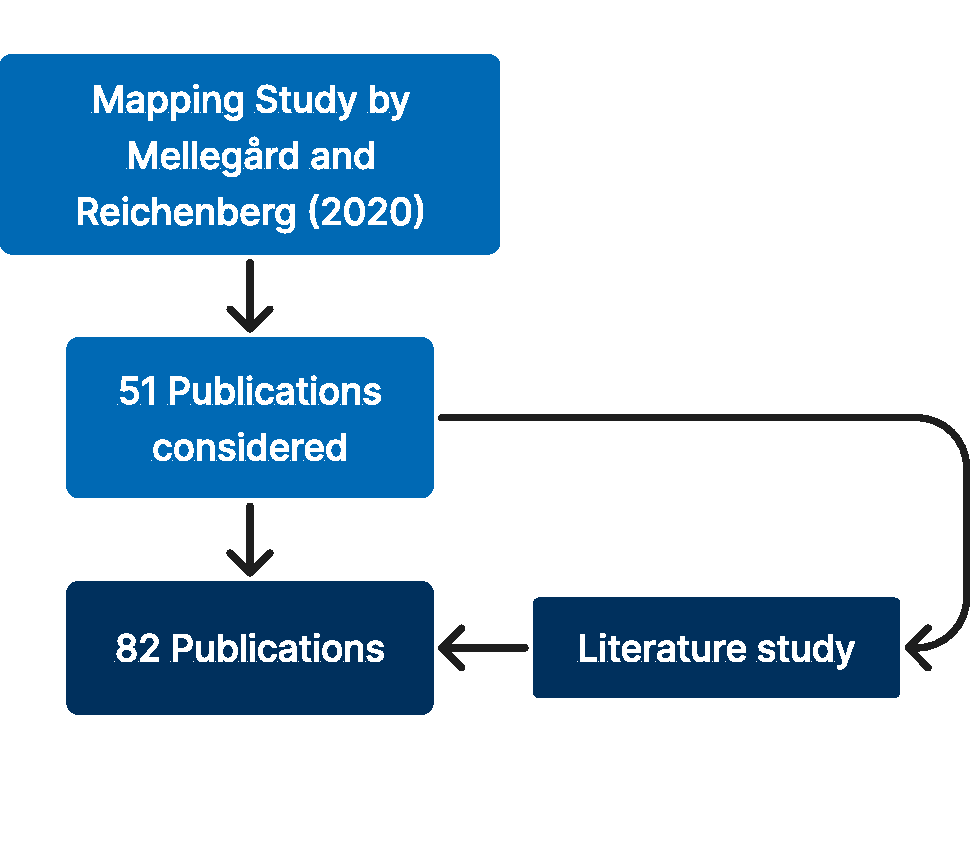
\includegraphics[width=\linewidth]{images/related-work-research-method.pdf} &
  \resizebox{\linewidth}{!}{%% Creator: Matplotlib, PGF backend
%%
%% To include the figure in your LaTeX document, write
%%   \input{<filename>.pgf}
%%
%% Make sure the required packages are loaded in your preamble
%%   \usepackage{pgf}
%%
%% Also ensure that all the required font packages are loaded; for instance,
%% the lmodern package is sometimes necessary when using math font.
%%   \usepackage{lmodern}
%%
%% Figures using additional raster images can only be included by \input if
%% they are in the same directory as the main LaTeX file. For loading figures
%% from other directories you can use the `import` package
%%   \usepackage{import}
%%
%% and then include the figures with
%%   \import{<path to file>}{<filename>.pgf}
%%
%% Matplotlib used the following preamble
%%   \def\mathdefault#1{#1}
%%   \everymath=\expandafter{\the\everymath\displaystyle}
%%   
%%   \makeatletter\@ifpackageloaded{underscore}{}{\usepackage[strings]{underscore}}\makeatother
%%
\begingroup%
\makeatletter%
\begin{pgfpicture}%
\pgfpathrectangle{\pgfpointorigin}{\pgfqpoint{4.490124in}{3.080266in}}%
\pgfusepath{use as bounding box, clip}%
\begin{pgfscope}%
\pgfsetbuttcap%
\pgfsetmiterjoin%
\definecolor{currentfill}{rgb}{1.000000,1.000000,1.000000}%
\pgfsetfillcolor{currentfill}%
\pgfsetlinewidth{0.000000pt}%
\definecolor{currentstroke}{rgb}{1.000000,1.000000,1.000000}%
\pgfsetstrokecolor{currentstroke}%
\pgfsetdash{}{0pt}%
\pgfpathmoveto{\pgfqpoint{0.000000in}{0.000000in}}%
\pgfpathlineto{\pgfqpoint{4.490124in}{0.000000in}}%
\pgfpathlineto{\pgfqpoint{4.490124in}{3.080266in}}%
\pgfpathlineto{\pgfqpoint{0.000000in}{3.080266in}}%
\pgfpathlineto{\pgfqpoint{0.000000in}{0.000000in}}%
\pgfpathclose%
\pgfusepath{fill}%
\end{pgfscope}%
\begin{pgfscope}%
\pgfsetbuttcap%
\pgfsetmiterjoin%
\definecolor{currentfill}{rgb}{1.000000,1.000000,1.000000}%
\pgfsetfillcolor{currentfill}%
\pgfsetlinewidth{0.000000pt}%
\definecolor{currentstroke}{rgb}{0.000000,0.000000,0.000000}%
\pgfsetstrokecolor{currentstroke}%
\pgfsetstrokeopacity{0.000000}%
\pgfsetdash{}{0pt}%
\pgfpathmoveto{\pgfqpoint{0.515124in}{0.622040in}}%
\pgfpathlineto{\pgfqpoint{4.390124in}{0.622040in}}%
\pgfpathlineto{\pgfqpoint{4.390124in}{2.932040in}}%
\pgfpathlineto{\pgfqpoint{0.515124in}{2.932040in}}%
\pgfpathlineto{\pgfqpoint{0.515124in}{0.622040in}}%
\pgfpathclose%
\pgfusepath{fill}%
\end{pgfscope}%
\begin{pgfscope}%
\pgfpathrectangle{\pgfqpoint{0.515124in}{0.622040in}}{\pgfqpoint{3.875000in}{2.310000in}}%
\pgfusepath{clip}%
\pgfsetbuttcap%
\pgfsetmiterjoin%
\definecolor{currentfill}{rgb}{0.400000,0.760784,0.647059}%
\pgfsetfillcolor{currentfill}%
\pgfsetlinewidth{0.000000pt}%
\definecolor{currentstroke}{rgb}{0.000000,0.000000,0.000000}%
\pgfsetstrokecolor{currentstroke}%
\pgfsetstrokeopacity{0.000000}%
\pgfsetdash{}{0pt}%
\pgfpathmoveto{\pgfqpoint{0.691260in}{0.622040in}}%
\pgfpathlineto{\pgfqpoint{0.840108in}{0.622040in}}%
\pgfpathlineto{\pgfqpoint{0.840108in}{0.853040in}}%
\pgfpathlineto{\pgfqpoint{0.691260in}{0.853040in}}%
\pgfpathlineto{\pgfqpoint{0.691260in}{0.622040in}}%
\pgfpathclose%
\pgfusepath{fill}%
\end{pgfscope}%
\begin{pgfscope}%
\pgfpathrectangle{\pgfqpoint{0.515124in}{0.622040in}}{\pgfqpoint{3.875000in}{2.310000in}}%
\pgfusepath{clip}%
\pgfsetbuttcap%
\pgfsetmiterjoin%
\definecolor{currentfill}{rgb}{0.400000,0.760784,0.647059}%
\pgfsetfillcolor{currentfill}%
\pgfsetlinewidth{0.000000pt}%
\definecolor{currentstroke}{rgb}{0.000000,0.000000,0.000000}%
\pgfsetstrokecolor{currentstroke}%
\pgfsetstrokeopacity{0.000000}%
\pgfsetdash{}{0pt}%
\pgfpathmoveto{\pgfqpoint{0.889724in}{0.622040in}}%
\pgfpathlineto{\pgfqpoint{1.038571in}{0.622040in}}%
\pgfpathlineto{\pgfqpoint{1.038571in}{0.622040in}}%
\pgfpathlineto{\pgfqpoint{0.889724in}{0.622040in}}%
\pgfpathlineto{\pgfqpoint{0.889724in}{0.622040in}}%
\pgfpathclose%
\pgfusepath{fill}%
\end{pgfscope}%
\begin{pgfscope}%
\pgfpathrectangle{\pgfqpoint{0.515124in}{0.622040in}}{\pgfqpoint{3.875000in}{2.310000in}}%
\pgfusepath{clip}%
\pgfsetbuttcap%
\pgfsetmiterjoin%
\definecolor{currentfill}{rgb}{0.400000,0.760784,0.647059}%
\pgfsetfillcolor{currentfill}%
\pgfsetlinewidth{0.000000pt}%
\definecolor{currentstroke}{rgb}{0.000000,0.000000,0.000000}%
\pgfsetstrokecolor{currentstroke}%
\pgfsetstrokeopacity{0.000000}%
\pgfsetdash{}{0pt}%
\pgfpathmoveto{\pgfqpoint{1.088187in}{0.622040in}}%
\pgfpathlineto{\pgfqpoint{1.237035in}{0.622040in}}%
\pgfpathlineto{\pgfqpoint{1.237035in}{0.853040in}}%
\pgfpathlineto{\pgfqpoint{1.088187in}{0.853040in}}%
\pgfpathlineto{\pgfqpoint{1.088187in}{0.622040in}}%
\pgfpathclose%
\pgfusepath{fill}%
\end{pgfscope}%
\begin{pgfscope}%
\pgfpathrectangle{\pgfqpoint{0.515124in}{0.622040in}}{\pgfqpoint{3.875000in}{2.310000in}}%
\pgfusepath{clip}%
\pgfsetbuttcap%
\pgfsetmiterjoin%
\definecolor{currentfill}{rgb}{0.400000,0.760784,0.647059}%
\pgfsetfillcolor{currentfill}%
\pgfsetlinewidth{0.000000pt}%
\definecolor{currentstroke}{rgb}{0.000000,0.000000,0.000000}%
\pgfsetstrokecolor{currentstroke}%
\pgfsetstrokeopacity{0.000000}%
\pgfsetdash{}{0pt}%
\pgfpathmoveto{\pgfqpoint{1.286651in}{0.622040in}}%
\pgfpathlineto{\pgfqpoint{1.435498in}{0.622040in}}%
\pgfpathlineto{\pgfqpoint{1.435498in}{0.622040in}}%
\pgfpathlineto{\pgfqpoint{1.286651in}{0.622040in}}%
\pgfpathlineto{\pgfqpoint{1.286651in}{0.622040in}}%
\pgfpathclose%
\pgfusepath{fill}%
\end{pgfscope}%
\begin{pgfscope}%
\pgfpathrectangle{\pgfqpoint{0.515124in}{0.622040in}}{\pgfqpoint{3.875000in}{2.310000in}}%
\pgfusepath{clip}%
\pgfsetbuttcap%
\pgfsetmiterjoin%
\definecolor{currentfill}{rgb}{0.400000,0.760784,0.647059}%
\pgfsetfillcolor{currentfill}%
\pgfsetlinewidth{0.000000pt}%
\definecolor{currentstroke}{rgb}{0.000000,0.000000,0.000000}%
\pgfsetstrokecolor{currentstroke}%
\pgfsetstrokeopacity{0.000000}%
\pgfsetdash{}{0pt}%
\pgfpathmoveto{\pgfqpoint{1.485114in}{0.622040in}}%
\pgfpathlineto{\pgfqpoint{1.633962in}{0.622040in}}%
\pgfpathlineto{\pgfqpoint{1.633962in}{0.853040in}}%
\pgfpathlineto{\pgfqpoint{1.485114in}{0.853040in}}%
\pgfpathlineto{\pgfqpoint{1.485114in}{0.622040in}}%
\pgfpathclose%
\pgfusepath{fill}%
\end{pgfscope}%
\begin{pgfscope}%
\pgfpathrectangle{\pgfqpoint{0.515124in}{0.622040in}}{\pgfqpoint{3.875000in}{2.310000in}}%
\pgfusepath{clip}%
\pgfsetbuttcap%
\pgfsetmiterjoin%
\definecolor{currentfill}{rgb}{0.400000,0.760784,0.647059}%
\pgfsetfillcolor{currentfill}%
\pgfsetlinewidth{0.000000pt}%
\definecolor{currentstroke}{rgb}{0.000000,0.000000,0.000000}%
\pgfsetstrokecolor{currentstroke}%
\pgfsetstrokeopacity{0.000000}%
\pgfsetdash{}{0pt}%
\pgfpathmoveto{\pgfqpoint{1.683578in}{0.622040in}}%
\pgfpathlineto{\pgfqpoint{1.832425in}{0.622040in}}%
\pgfpathlineto{\pgfqpoint{1.832425in}{2.239040in}}%
\pgfpathlineto{\pgfqpoint{1.683578in}{2.239040in}}%
\pgfpathlineto{\pgfqpoint{1.683578in}{0.622040in}}%
\pgfpathclose%
\pgfusepath{fill}%
\end{pgfscope}%
\begin{pgfscope}%
\pgfpathrectangle{\pgfqpoint{0.515124in}{0.622040in}}{\pgfqpoint{3.875000in}{2.310000in}}%
\pgfusepath{clip}%
\pgfsetbuttcap%
\pgfsetmiterjoin%
\definecolor{currentfill}{rgb}{0.400000,0.760784,0.647059}%
\pgfsetfillcolor{currentfill}%
\pgfsetlinewidth{0.000000pt}%
\definecolor{currentstroke}{rgb}{0.000000,0.000000,0.000000}%
\pgfsetstrokecolor{currentstroke}%
\pgfsetstrokeopacity{0.000000}%
\pgfsetdash{}{0pt}%
\pgfpathmoveto{\pgfqpoint{1.882041in}{0.622040in}}%
\pgfpathlineto{\pgfqpoint{2.030889in}{0.622040in}}%
\pgfpathlineto{\pgfqpoint{2.030889in}{2.008040in}}%
\pgfpathlineto{\pgfqpoint{1.882041in}{2.008040in}}%
\pgfpathlineto{\pgfqpoint{1.882041in}{0.622040in}}%
\pgfpathclose%
\pgfusepath{fill}%
\end{pgfscope}%
\begin{pgfscope}%
\pgfpathrectangle{\pgfqpoint{0.515124in}{0.622040in}}{\pgfqpoint{3.875000in}{2.310000in}}%
\pgfusepath{clip}%
\pgfsetbuttcap%
\pgfsetmiterjoin%
\definecolor{currentfill}{rgb}{0.400000,0.760784,0.647059}%
\pgfsetfillcolor{currentfill}%
\pgfsetlinewidth{0.000000pt}%
\definecolor{currentstroke}{rgb}{0.000000,0.000000,0.000000}%
\pgfsetstrokecolor{currentstroke}%
\pgfsetstrokeopacity{0.000000}%
\pgfsetdash{}{0pt}%
\pgfpathmoveto{\pgfqpoint{2.080505in}{0.622040in}}%
\pgfpathlineto{\pgfqpoint{2.229352in}{0.622040in}}%
\pgfpathlineto{\pgfqpoint{2.229352in}{2.239040in}}%
\pgfpathlineto{\pgfqpoint{2.080505in}{2.239040in}}%
\pgfpathlineto{\pgfqpoint{2.080505in}{0.622040in}}%
\pgfpathclose%
\pgfusepath{fill}%
\end{pgfscope}%
\begin{pgfscope}%
\pgfpathrectangle{\pgfqpoint{0.515124in}{0.622040in}}{\pgfqpoint{3.875000in}{2.310000in}}%
\pgfusepath{clip}%
\pgfsetbuttcap%
\pgfsetmiterjoin%
\definecolor{currentfill}{rgb}{0.400000,0.760784,0.647059}%
\pgfsetfillcolor{currentfill}%
\pgfsetlinewidth{0.000000pt}%
\definecolor{currentstroke}{rgb}{0.000000,0.000000,0.000000}%
\pgfsetstrokecolor{currentstroke}%
\pgfsetstrokeopacity{0.000000}%
\pgfsetdash{}{0pt}%
\pgfpathmoveto{\pgfqpoint{2.278968in}{0.622040in}}%
\pgfpathlineto{\pgfqpoint{2.427816in}{0.622040in}}%
\pgfpathlineto{\pgfqpoint{2.427816in}{1.777040in}}%
\pgfpathlineto{\pgfqpoint{2.278968in}{1.777040in}}%
\pgfpathlineto{\pgfqpoint{2.278968in}{0.622040in}}%
\pgfpathclose%
\pgfusepath{fill}%
\end{pgfscope}%
\begin{pgfscope}%
\pgfpathrectangle{\pgfqpoint{0.515124in}{0.622040in}}{\pgfqpoint{3.875000in}{2.310000in}}%
\pgfusepath{clip}%
\pgfsetbuttcap%
\pgfsetmiterjoin%
\definecolor{currentfill}{rgb}{0.400000,0.760784,0.647059}%
\pgfsetfillcolor{currentfill}%
\pgfsetlinewidth{0.000000pt}%
\definecolor{currentstroke}{rgb}{0.000000,0.000000,0.000000}%
\pgfsetstrokecolor{currentstroke}%
\pgfsetstrokeopacity{0.000000}%
\pgfsetdash{}{0pt}%
\pgfpathmoveto{\pgfqpoint{2.477432in}{0.622040in}}%
\pgfpathlineto{\pgfqpoint{2.626279in}{0.622040in}}%
\pgfpathlineto{\pgfqpoint{2.626279in}{1.084040in}}%
\pgfpathlineto{\pgfqpoint{2.477432in}{1.084040in}}%
\pgfpathlineto{\pgfqpoint{2.477432in}{0.622040in}}%
\pgfpathclose%
\pgfusepath{fill}%
\end{pgfscope}%
\begin{pgfscope}%
\pgfpathrectangle{\pgfqpoint{0.515124in}{0.622040in}}{\pgfqpoint{3.875000in}{2.310000in}}%
\pgfusepath{clip}%
\pgfsetbuttcap%
\pgfsetmiterjoin%
\definecolor{currentfill}{rgb}{0.400000,0.760784,0.647059}%
\pgfsetfillcolor{currentfill}%
\pgfsetlinewidth{0.000000pt}%
\definecolor{currentstroke}{rgb}{0.000000,0.000000,0.000000}%
\pgfsetstrokecolor{currentstroke}%
\pgfsetstrokeopacity{0.000000}%
\pgfsetdash{}{0pt}%
\pgfpathmoveto{\pgfqpoint{2.675895in}{0.622040in}}%
\pgfpathlineto{\pgfqpoint{2.824743in}{0.622040in}}%
\pgfpathlineto{\pgfqpoint{2.824743in}{1.777040in}}%
\pgfpathlineto{\pgfqpoint{2.675895in}{1.777040in}}%
\pgfpathlineto{\pgfqpoint{2.675895in}{0.622040in}}%
\pgfpathclose%
\pgfusepath{fill}%
\end{pgfscope}%
\begin{pgfscope}%
\pgfpathrectangle{\pgfqpoint{0.515124in}{0.622040in}}{\pgfqpoint{3.875000in}{2.310000in}}%
\pgfusepath{clip}%
\pgfsetbuttcap%
\pgfsetmiterjoin%
\definecolor{currentfill}{rgb}{0.400000,0.760784,0.647059}%
\pgfsetfillcolor{currentfill}%
\pgfsetlinewidth{0.000000pt}%
\definecolor{currentstroke}{rgb}{0.000000,0.000000,0.000000}%
\pgfsetstrokecolor{currentstroke}%
\pgfsetstrokeopacity{0.000000}%
\pgfsetdash{}{0pt}%
\pgfpathmoveto{\pgfqpoint{2.874359in}{0.622040in}}%
\pgfpathlineto{\pgfqpoint{3.023206in}{0.622040in}}%
\pgfpathlineto{\pgfqpoint{3.023206in}{1.084040in}}%
\pgfpathlineto{\pgfqpoint{2.874359in}{1.084040in}}%
\pgfpathlineto{\pgfqpoint{2.874359in}{0.622040in}}%
\pgfpathclose%
\pgfusepath{fill}%
\end{pgfscope}%
\begin{pgfscope}%
\pgfpathrectangle{\pgfqpoint{0.515124in}{0.622040in}}{\pgfqpoint{3.875000in}{2.310000in}}%
\pgfusepath{clip}%
\pgfsetbuttcap%
\pgfsetmiterjoin%
\definecolor{currentfill}{rgb}{0.400000,0.760784,0.647059}%
\pgfsetfillcolor{currentfill}%
\pgfsetlinewidth{0.000000pt}%
\definecolor{currentstroke}{rgb}{0.000000,0.000000,0.000000}%
\pgfsetstrokecolor{currentstroke}%
\pgfsetstrokeopacity{0.000000}%
\pgfsetdash{}{0pt}%
\pgfpathmoveto{\pgfqpoint{3.072822in}{0.622040in}}%
\pgfpathlineto{\pgfqpoint{3.221670in}{0.622040in}}%
\pgfpathlineto{\pgfqpoint{3.221670in}{2.239040in}}%
\pgfpathlineto{\pgfqpoint{3.072822in}{2.239040in}}%
\pgfpathlineto{\pgfqpoint{3.072822in}{0.622040in}}%
\pgfpathclose%
\pgfusepath{fill}%
\end{pgfscope}%
\begin{pgfscope}%
\pgfpathrectangle{\pgfqpoint{0.515124in}{0.622040in}}{\pgfqpoint{3.875000in}{2.310000in}}%
\pgfusepath{clip}%
\pgfsetbuttcap%
\pgfsetmiterjoin%
\definecolor{currentfill}{rgb}{0.400000,0.760784,0.647059}%
\pgfsetfillcolor{currentfill}%
\pgfsetlinewidth{0.000000pt}%
\definecolor{currentstroke}{rgb}{0.000000,0.000000,0.000000}%
\pgfsetstrokecolor{currentstroke}%
\pgfsetstrokeopacity{0.000000}%
\pgfsetdash{}{0pt}%
\pgfpathmoveto{\pgfqpoint{3.271286in}{0.622040in}}%
\pgfpathlineto{\pgfqpoint{3.420133in}{0.622040in}}%
\pgfpathlineto{\pgfqpoint{3.420133in}{1.084040in}}%
\pgfpathlineto{\pgfqpoint{3.271286in}{1.084040in}}%
\pgfpathlineto{\pgfqpoint{3.271286in}{0.622040in}}%
\pgfpathclose%
\pgfusepath{fill}%
\end{pgfscope}%
\begin{pgfscope}%
\pgfpathrectangle{\pgfqpoint{0.515124in}{0.622040in}}{\pgfqpoint{3.875000in}{2.310000in}}%
\pgfusepath{clip}%
\pgfsetbuttcap%
\pgfsetmiterjoin%
\definecolor{currentfill}{rgb}{0.400000,0.760784,0.647059}%
\pgfsetfillcolor{currentfill}%
\pgfsetlinewidth{0.000000pt}%
\definecolor{currentstroke}{rgb}{0.000000,0.000000,0.000000}%
\pgfsetstrokecolor{currentstroke}%
\pgfsetstrokeopacity{0.000000}%
\pgfsetdash{}{0pt}%
\pgfpathmoveto{\pgfqpoint{3.469749in}{0.622040in}}%
\pgfpathlineto{\pgfqpoint{3.618597in}{0.622040in}}%
\pgfpathlineto{\pgfqpoint{3.618597in}{0.622040in}}%
\pgfpathlineto{\pgfqpoint{3.469749in}{0.622040in}}%
\pgfpathlineto{\pgfqpoint{3.469749in}{0.622040in}}%
\pgfpathclose%
\pgfusepath{fill}%
\end{pgfscope}%
\begin{pgfscope}%
\pgfpathrectangle{\pgfqpoint{0.515124in}{0.622040in}}{\pgfqpoint{3.875000in}{2.310000in}}%
\pgfusepath{clip}%
\pgfsetbuttcap%
\pgfsetmiterjoin%
\definecolor{currentfill}{rgb}{0.400000,0.760784,0.647059}%
\pgfsetfillcolor{currentfill}%
\pgfsetlinewidth{0.000000pt}%
\definecolor{currentstroke}{rgb}{0.000000,0.000000,0.000000}%
\pgfsetstrokecolor{currentstroke}%
\pgfsetstrokeopacity{0.000000}%
\pgfsetdash{}{0pt}%
\pgfpathmoveto{\pgfqpoint{3.668213in}{0.622040in}}%
\pgfpathlineto{\pgfqpoint{3.817060in}{0.622040in}}%
\pgfpathlineto{\pgfqpoint{3.817060in}{0.622040in}}%
\pgfpathlineto{\pgfqpoint{3.668213in}{0.622040in}}%
\pgfpathlineto{\pgfqpoint{3.668213in}{0.622040in}}%
\pgfpathclose%
\pgfusepath{fill}%
\end{pgfscope}%
\begin{pgfscope}%
\pgfpathrectangle{\pgfqpoint{0.515124in}{0.622040in}}{\pgfqpoint{3.875000in}{2.310000in}}%
\pgfusepath{clip}%
\pgfsetbuttcap%
\pgfsetmiterjoin%
\definecolor{currentfill}{rgb}{0.400000,0.760784,0.647059}%
\pgfsetfillcolor{currentfill}%
\pgfsetlinewidth{0.000000pt}%
\definecolor{currentstroke}{rgb}{0.000000,0.000000,0.000000}%
\pgfsetstrokecolor{currentstroke}%
\pgfsetstrokeopacity{0.000000}%
\pgfsetdash{}{0pt}%
\pgfpathmoveto{\pgfqpoint{3.866676in}{0.622040in}}%
\pgfpathlineto{\pgfqpoint{4.015524in}{0.622040in}}%
\pgfpathlineto{\pgfqpoint{4.015524in}{0.622040in}}%
\pgfpathlineto{\pgfqpoint{3.866676in}{0.622040in}}%
\pgfpathlineto{\pgfqpoint{3.866676in}{0.622040in}}%
\pgfpathclose%
\pgfusepath{fill}%
\end{pgfscope}%
\begin{pgfscope}%
\pgfpathrectangle{\pgfqpoint{0.515124in}{0.622040in}}{\pgfqpoint{3.875000in}{2.310000in}}%
\pgfusepath{clip}%
\pgfsetbuttcap%
\pgfsetmiterjoin%
\definecolor{currentfill}{rgb}{0.400000,0.760784,0.647059}%
\pgfsetfillcolor{currentfill}%
\pgfsetlinewidth{0.000000pt}%
\definecolor{currentstroke}{rgb}{0.000000,0.000000,0.000000}%
\pgfsetstrokecolor{currentstroke}%
\pgfsetstrokeopacity{0.000000}%
\pgfsetdash{}{0pt}%
\pgfpathmoveto{\pgfqpoint{4.065140in}{0.622040in}}%
\pgfpathlineto{\pgfqpoint{4.213987in}{0.622040in}}%
\pgfpathlineto{\pgfqpoint{4.213987in}{0.622040in}}%
\pgfpathlineto{\pgfqpoint{4.065140in}{0.622040in}}%
\pgfpathlineto{\pgfqpoint{4.065140in}{0.622040in}}%
\pgfpathclose%
\pgfusepath{fill}%
\end{pgfscope}%
\begin{pgfscope}%
\pgfpathrectangle{\pgfqpoint{0.515124in}{0.622040in}}{\pgfqpoint{3.875000in}{2.310000in}}%
\pgfusepath{clip}%
\pgfsetbuttcap%
\pgfsetmiterjoin%
\definecolor{currentfill}{rgb}{0.988235,0.552941,0.384314}%
\pgfsetfillcolor{currentfill}%
\pgfsetlinewidth{0.000000pt}%
\definecolor{currentstroke}{rgb}{0.000000,0.000000,0.000000}%
\pgfsetstrokecolor{currentstroke}%
\pgfsetstrokeopacity{0.000000}%
\pgfsetdash{}{0pt}%
\pgfpathmoveto{\pgfqpoint{0.691260in}{0.853040in}}%
\pgfpathlineto{\pgfqpoint{0.840108in}{0.853040in}}%
\pgfpathlineto{\pgfqpoint{0.840108in}{0.853040in}}%
\pgfpathlineto{\pgfqpoint{0.691260in}{0.853040in}}%
\pgfpathlineto{\pgfqpoint{0.691260in}{0.853040in}}%
\pgfpathclose%
\pgfusepath{fill}%
\end{pgfscope}%
\begin{pgfscope}%
\pgfpathrectangle{\pgfqpoint{0.515124in}{0.622040in}}{\pgfqpoint{3.875000in}{2.310000in}}%
\pgfusepath{clip}%
\pgfsetbuttcap%
\pgfsetmiterjoin%
\definecolor{currentfill}{rgb}{0.988235,0.552941,0.384314}%
\pgfsetfillcolor{currentfill}%
\pgfsetlinewidth{0.000000pt}%
\definecolor{currentstroke}{rgb}{0.000000,0.000000,0.000000}%
\pgfsetstrokecolor{currentstroke}%
\pgfsetstrokeopacity{0.000000}%
\pgfsetdash{}{0pt}%
\pgfpathmoveto{\pgfqpoint{0.889724in}{0.622040in}}%
\pgfpathlineto{\pgfqpoint{1.038571in}{0.622040in}}%
\pgfpathlineto{\pgfqpoint{1.038571in}{0.622040in}}%
\pgfpathlineto{\pgfqpoint{0.889724in}{0.622040in}}%
\pgfpathlineto{\pgfqpoint{0.889724in}{0.622040in}}%
\pgfpathclose%
\pgfusepath{fill}%
\end{pgfscope}%
\begin{pgfscope}%
\pgfpathrectangle{\pgfqpoint{0.515124in}{0.622040in}}{\pgfqpoint{3.875000in}{2.310000in}}%
\pgfusepath{clip}%
\pgfsetbuttcap%
\pgfsetmiterjoin%
\definecolor{currentfill}{rgb}{0.988235,0.552941,0.384314}%
\pgfsetfillcolor{currentfill}%
\pgfsetlinewidth{0.000000pt}%
\definecolor{currentstroke}{rgb}{0.000000,0.000000,0.000000}%
\pgfsetstrokecolor{currentstroke}%
\pgfsetstrokeopacity{0.000000}%
\pgfsetdash{}{0pt}%
\pgfpathmoveto{\pgfqpoint{1.088187in}{0.853040in}}%
\pgfpathlineto{\pgfqpoint{1.237035in}{0.853040in}}%
\pgfpathlineto{\pgfqpoint{1.237035in}{0.853040in}}%
\pgfpathlineto{\pgfqpoint{1.088187in}{0.853040in}}%
\pgfpathlineto{\pgfqpoint{1.088187in}{0.853040in}}%
\pgfpathclose%
\pgfusepath{fill}%
\end{pgfscope}%
\begin{pgfscope}%
\pgfpathrectangle{\pgfqpoint{0.515124in}{0.622040in}}{\pgfqpoint{3.875000in}{2.310000in}}%
\pgfusepath{clip}%
\pgfsetbuttcap%
\pgfsetmiterjoin%
\definecolor{currentfill}{rgb}{0.988235,0.552941,0.384314}%
\pgfsetfillcolor{currentfill}%
\pgfsetlinewidth{0.000000pt}%
\definecolor{currentstroke}{rgb}{0.000000,0.000000,0.000000}%
\pgfsetstrokecolor{currentstroke}%
\pgfsetstrokeopacity{0.000000}%
\pgfsetdash{}{0pt}%
\pgfpathmoveto{\pgfqpoint{1.286651in}{0.622040in}}%
\pgfpathlineto{\pgfqpoint{1.435498in}{0.622040in}}%
\pgfpathlineto{\pgfqpoint{1.435498in}{0.622040in}}%
\pgfpathlineto{\pgfqpoint{1.286651in}{0.622040in}}%
\pgfpathlineto{\pgfqpoint{1.286651in}{0.622040in}}%
\pgfpathclose%
\pgfusepath{fill}%
\end{pgfscope}%
\begin{pgfscope}%
\pgfpathrectangle{\pgfqpoint{0.515124in}{0.622040in}}{\pgfqpoint{3.875000in}{2.310000in}}%
\pgfusepath{clip}%
\pgfsetbuttcap%
\pgfsetmiterjoin%
\definecolor{currentfill}{rgb}{0.988235,0.552941,0.384314}%
\pgfsetfillcolor{currentfill}%
\pgfsetlinewidth{0.000000pt}%
\definecolor{currentstroke}{rgb}{0.000000,0.000000,0.000000}%
\pgfsetstrokecolor{currentstroke}%
\pgfsetstrokeopacity{0.000000}%
\pgfsetdash{}{0pt}%
\pgfpathmoveto{\pgfqpoint{1.485114in}{0.853040in}}%
\pgfpathlineto{\pgfqpoint{1.633962in}{0.853040in}}%
\pgfpathlineto{\pgfqpoint{1.633962in}{1.084040in}}%
\pgfpathlineto{\pgfqpoint{1.485114in}{1.084040in}}%
\pgfpathlineto{\pgfqpoint{1.485114in}{0.853040in}}%
\pgfpathclose%
\pgfusepath{fill}%
\end{pgfscope}%
\begin{pgfscope}%
\pgfpathrectangle{\pgfqpoint{0.515124in}{0.622040in}}{\pgfqpoint{3.875000in}{2.310000in}}%
\pgfusepath{clip}%
\pgfsetbuttcap%
\pgfsetmiterjoin%
\definecolor{currentfill}{rgb}{0.988235,0.552941,0.384314}%
\pgfsetfillcolor{currentfill}%
\pgfsetlinewidth{0.000000pt}%
\definecolor{currentstroke}{rgb}{0.000000,0.000000,0.000000}%
\pgfsetstrokecolor{currentstroke}%
\pgfsetstrokeopacity{0.000000}%
\pgfsetdash{}{0pt}%
\pgfpathmoveto{\pgfqpoint{1.683578in}{2.239040in}}%
\pgfpathlineto{\pgfqpoint{1.832425in}{2.239040in}}%
\pgfpathlineto{\pgfqpoint{1.832425in}{2.239040in}}%
\pgfpathlineto{\pgfqpoint{1.683578in}{2.239040in}}%
\pgfpathlineto{\pgfqpoint{1.683578in}{2.239040in}}%
\pgfpathclose%
\pgfusepath{fill}%
\end{pgfscope}%
\begin{pgfscope}%
\pgfpathrectangle{\pgfqpoint{0.515124in}{0.622040in}}{\pgfqpoint{3.875000in}{2.310000in}}%
\pgfusepath{clip}%
\pgfsetbuttcap%
\pgfsetmiterjoin%
\definecolor{currentfill}{rgb}{0.988235,0.552941,0.384314}%
\pgfsetfillcolor{currentfill}%
\pgfsetlinewidth{0.000000pt}%
\definecolor{currentstroke}{rgb}{0.000000,0.000000,0.000000}%
\pgfsetstrokecolor{currentstroke}%
\pgfsetstrokeopacity{0.000000}%
\pgfsetdash{}{0pt}%
\pgfpathmoveto{\pgfqpoint{1.882041in}{2.008040in}}%
\pgfpathlineto{\pgfqpoint{2.030889in}{2.008040in}}%
\pgfpathlineto{\pgfqpoint{2.030889in}{2.239040in}}%
\pgfpathlineto{\pgfqpoint{1.882041in}{2.239040in}}%
\pgfpathlineto{\pgfqpoint{1.882041in}{2.008040in}}%
\pgfpathclose%
\pgfusepath{fill}%
\end{pgfscope}%
\begin{pgfscope}%
\pgfpathrectangle{\pgfqpoint{0.515124in}{0.622040in}}{\pgfqpoint{3.875000in}{2.310000in}}%
\pgfusepath{clip}%
\pgfsetbuttcap%
\pgfsetmiterjoin%
\definecolor{currentfill}{rgb}{0.988235,0.552941,0.384314}%
\pgfsetfillcolor{currentfill}%
\pgfsetlinewidth{0.000000pt}%
\definecolor{currentstroke}{rgb}{0.000000,0.000000,0.000000}%
\pgfsetstrokecolor{currentstroke}%
\pgfsetstrokeopacity{0.000000}%
\pgfsetdash{}{0pt}%
\pgfpathmoveto{\pgfqpoint{2.080505in}{2.239040in}}%
\pgfpathlineto{\pgfqpoint{2.229352in}{2.239040in}}%
\pgfpathlineto{\pgfqpoint{2.229352in}{2.239040in}}%
\pgfpathlineto{\pgfqpoint{2.080505in}{2.239040in}}%
\pgfpathlineto{\pgfqpoint{2.080505in}{2.239040in}}%
\pgfpathclose%
\pgfusepath{fill}%
\end{pgfscope}%
\begin{pgfscope}%
\pgfpathrectangle{\pgfqpoint{0.515124in}{0.622040in}}{\pgfqpoint{3.875000in}{2.310000in}}%
\pgfusepath{clip}%
\pgfsetbuttcap%
\pgfsetmiterjoin%
\definecolor{currentfill}{rgb}{0.988235,0.552941,0.384314}%
\pgfsetfillcolor{currentfill}%
\pgfsetlinewidth{0.000000pt}%
\definecolor{currentstroke}{rgb}{0.000000,0.000000,0.000000}%
\pgfsetstrokecolor{currentstroke}%
\pgfsetstrokeopacity{0.000000}%
\pgfsetdash{}{0pt}%
\pgfpathmoveto{\pgfqpoint{2.278968in}{1.777040in}}%
\pgfpathlineto{\pgfqpoint{2.427816in}{1.777040in}}%
\pgfpathlineto{\pgfqpoint{2.427816in}{1.777040in}}%
\pgfpathlineto{\pgfqpoint{2.278968in}{1.777040in}}%
\pgfpathlineto{\pgfqpoint{2.278968in}{1.777040in}}%
\pgfpathclose%
\pgfusepath{fill}%
\end{pgfscope}%
\begin{pgfscope}%
\pgfpathrectangle{\pgfqpoint{0.515124in}{0.622040in}}{\pgfqpoint{3.875000in}{2.310000in}}%
\pgfusepath{clip}%
\pgfsetbuttcap%
\pgfsetmiterjoin%
\definecolor{currentfill}{rgb}{0.988235,0.552941,0.384314}%
\pgfsetfillcolor{currentfill}%
\pgfsetlinewidth{0.000000pt}%
\definecolor{currentstroke}{rgb}{0.000000,0.000000,0.000000}%
\pgfsetstrokecolor{currentstroke}%
\pgfsetstrokeopacity{0.000000}%
\pgfsetdash{}{0pt}%
\pgfpathmoveto{\pgfqpoint{2.477432in}{1.084040in}}%
\pgfpathlineto{\pgfqpoint{2.626279in}{1.084040in}}%
\pgfpathlineto{\pgfqpoint{2.626279in}{1.315040in}}%
\pgfpathlineto{\pgfqpoint{2.477432in}{1.315040in}}%
\pgfpathlineto{\pgfqpoint{2.477432in}{1.084040in}}%
\pgfpathclose%
\pgfusepath{fill}%
\end{pgfscope}%
\begin{pgfscope}%
\pgfpathrectangle{\pgfqpoint{0.515124in}{0.622040in}}{\pgfqpoint{3.875000in}{2.310000in}}%
\pgfusepath{clip}%
\pgfsetbuttcap%
\pgfsetmiterjoin%
\definecolor{currentfill}{rgb}{0.988235,0.552941,0.384314}%
\pgfsetfillcolor{currentfill}%
\pgfsetlinewidth{0.000000pt}%
\definecolor{currentstroke}{rgb}{0.000000,0.000000,0.000000}%
\pgfsetstrokecolor{currentstroke}%
\pgfsetstrokeopacity{0.000000}%
\pgfsetdash{}{0pt}%
\pgfpathmoveto{\pgfqpoint{2.675895in}{1.777040in}}%
\pgfpathlineto{\pgfqpoint{2.824743in}{1.777040in}}%
\pgfpathlineto{\pgfqpoint{2.824743in}{1.777040in}}%
\pgfpathlineto{\pgfqpoint{2.675895in}{1.777040in}}%
\pgfpathlineto{\pgfqpoint{2.675895in}{1.777040in}}%
\pgfpathclose%
\pgfusepath{fill}%
\end{pgfscope}%
\begin{pgfscope}%
\pgfpathrectangle{\pgfqpoint{0.515124in}{0.622040in}}{\pgfqpoint{3.875000in}{2.310000in}}%
\pgfusepath{clip}%
\pgfsetbuttcap%
\pgfsetmiterjoin%
\definecolor{currentfill}{rgb}{0.988235,0.552941,0.384314}%
\pgfsetfillcolor{currentfill}%
\pgfsetlinewidth{0.000000pt}%
\definecolor{currentstroke}{rgb}{0.000000,0.000000,0.000000}%
\pgfsetstrokecolor{currentstroke}%
\pgfsetstrokeopacity{0.000000}%
\pgfsetdash{}{0pt}%
\pgfpathmoveto{\pgfqpoint{2.874359in}{1.084040in}}%
\pgfpathlineto{\pgfqpoint{3.023206in}{1.084040in}}%
\pgfpathlineto{\pgfqpoint{3.023206in}{1.546040in}}%
\pgfpathlineto{\pgfqpoint{2.874359in}{1.546040in}}%
\pgfpathlineto{\pgfqpoint{2.874359in}{1.084040in}}%
\pgfpathclose%
\pgfusepath{fill}%
\end{pgfscope}%
\begin{pgfscope}%
\pgfpathrectangle{\pgfqpoint{0.515124in}{0.622040in}}{\pgfqpoint{3.875000in}{2.310000in}}%
\pgfusepath{clip}%
\pgfsetbuttcap%
\pgfsetmiterjoin%
\definecolor{currentfill}{rgb}{0.988235,0.552941,0.384314}%
\pgfsetfillcolor{currentfill}%
\pgfsetlinewidth{0.000000pt}%
\definecolor{currentstroke}{rgb}{0.000000,0.000000,0.000000}%
\pgfsetstrokecolor{currentstroke}%
\pgfsetstrokeopacity{0.000000}%
\pgfsetdash{}{0pt}%
\pgfpathmoveto{\pgfqpoint{3.072822in}{2.239040in}}%
\pgfpathlineto{\pgfqpoint{3.221670in}{2.239040in}}%
\pgfpathlineto{\pgfqpoint{3.221670in}{2.470040in}}%
\pgfpathlineto{\pgfqpoint{3.072822in}{2.470040in}}%
\pgfpathlineto{\pgfqpoint{3.072822in}{2.239040in}}%
\pgfpathclose%
\pgfusepath{fill}%
\end{pgfscope}%
\begin{pgfscope}%
\pgfpathrectangle{\pgfqpoint{0.515124in}{0.622040in}}{\pgfqpoint{3.875000in}{2.310000in}}%
\pgfusepath{clip}%
\pgfsetbuttcap%
\pgfsetmiterjoin%
\definecolor{currentfill}{rgb}{0.988235,0.552941,0.384314}%
\pgfsetfillcolor{currentfill}%
\pgfsetlinewidth{0.000000pt}%
\definecolor{currentstroke}{rgb}{0.000000,0.000000,0.000000}%
\pgfsetstrokecolor{currentstroke}%
\pgfsetstrokeopacity{0.000000}%
\pgfsetdash{}{0pt}%
\pgfpathmoveto{\pgfqpoint{3.271286in}{1.084040in}}%
\pgfpathlineto{\pgfqpoint{3.420133in}{1.084040in}}%
\pgfpathlineto{\pgfqpoint{3.420133in}{1.777040in}}%
\pgfpathlineto{\pgfqpoint{3.271286in}{1.777040in}}%
\pgfpathlineto{\pgfqpoint{3.271286in}{1.084040in}}%
\pgfpathclose%
\pgfusepath{fill}%
\end{pgfscope}%
\begin{pgfscope}%
\pgfpathrectangle{\pgfqpoint{0.515124in}{0.622040in}}{\pgfqpoint{3.875000in}{2.310000in}}%
\pgfusepath{clip}%
\pgfsetbuttcap%
\pgfsetmiterjoin%
\definecolor{currentfill}{rgb}{0.988235,0.552941,0.384314}%
\pgfsetfillcolor{currentfill}%
\pgfsetlinewidth{0.000000pt}%
\definecolor{currentstroke}{rgb}{0.000000,0.000000,0.000000}%
\pgfsetstrokecolor{currentstroke}%
\pgfsetstrokeopacity{0.000000}%
\pgfsetdash{}{0pt}%
\pgfpathmoveto{\pgfqpoint{3.469749in}{0.622040in}}%
\pgfpathlineto{\pgfqpoint{3.618597in}{0.622040in}}%
\pgfpathlineto{\pgfqpoint{3.618597in}{1.777040in}}%
\pgfpathlineto{\pgfqpoint{3.469749in}{1.777040in}}%
\pgfpathlineto{\pgfqpoint{3.469749in}{0.622040in}}%
\pgfpathclose%
\pgfusepath{fill}%
\end{pgfscope}%
\begin{pgfscope}%
\pgfpathrectangle{\pgfqpoint{0.515124in}{0.622040in}}{\pgfqpoint{3.875000in}{2.310000in}}%
\pgfusepath{clip}%
\pgfsetbuttcap%
\pgfsetmiterjoin%
\definecolor{currentfill}{rgb}{0.988235,0.552941,0.384314}%
\pgfsetfillcolor{currentfill}%
\pgfsetlinewidth{0.000000pt}%
\definecolor{currentstroke}{rgb}{0.000000,0.000000,0.000000}%
\pgfsetstrokecolor{currentstroke}%
\pgfsetstrokeopacity{0.000000}%
\pgfsetdash{}{0pt}%
\pgfpathmoveto{\pgfqpoint{3.668213in}{0.622040in}}%
\pgfpathlineto{\pgfqpoint{3.817060in}{0.622040in}}%
\pgfpathlineto{\pgfqpoint{3.817060in}{1.315040in}}%
\pgfpathlineto{\pgfqpoint{3.668213in}{1.315040in}}%
\pgfpathlineto{\pgfqpoint{3.668213in}{0.622040in}}%
\pgfpathclose%
\pgfusepath{fill}%
\end{pgfscope}%
\begin{pgfscope}%
\pgfpathrectangle{\pgfqpoint{0.515124in}{0.622040in}}{\pgfqpoint{3.875000in}{2.310000in}}%
\pgfusepath{clip}%
\pgfsetbuttcap%
\pgfsetmiterjoin%
\definecolor{currentfill}{rgb}{0.988235,0.552941,0.384314}%
\pgfsetfillcolor{currentfill}%
\pgfsetlinewidth{0.000000pt}%
\definecolor{currentstroke}{rgb}{0.000000,0.000000,0.000000}%
\pgfsetstrokecolor{currentstroke}%
\pgfsetstrokeopacity{0.000000}%
\pgfsetdash{}{0pt}%
\pgfpathmoveto{\pgfqpoint{3.866676in}{0.622040in}}%
\pgfpathlineto{\pgfqpoint{4.015524in}{0.622040in}}%
\pgfpathlineto{\pgfqpoint{4.015524in}{1.315040in}}%
\pgfpathlineto{\pgfqpoint{3.866676in}{1.315040in}}%
\pgfpathlineto{\pgfqpoint{3.866676in}{0.622040in}}%
\pgfpathclose%
\pgfusepath{fill}%
\end{pgfscope}%
\begin{pgfscope}%
\pgfpathrectangle{\pgfqpoint{0.515124in}{0.622040in}}{\pgfqpoint{3.875000in}{2.310000in}}%
\pgfusepath{clip}%
\pgfsetbuttcap%
\pgfsetmiterjoin%
\definecolor{currentfill}{rgb}{0.988235,0.552941,0.384314}%
\pgfsetfillcolor{currentfill}%
\pgfsetlinewidth{0.000000pt}%
\definecolor{currentstroke}{rgb}{0.000000,0.000000,0.000000}%
\pgfsetstrokecolor{currentstroke}%
\pgfsetstrokeopacity{0.000000}%
\pgfsetdash{}{0pt}%
\pgfpathmoveto{\pgfqpoint{4.065140in}{0.622040in}}%
\pgfpathlineto{\pgfqpoint{4.213987in}{0.622040in}}%
\pgfpathlineto{\pgfqpoint{4.213987in}{1.777040in}}%
\pgfpathlineto{\pgfqpoint{4.065140in}{1.777040in}}%
\pgfpathlineto{\pgfqpoint{4.065140in}{0.622040in}}%
\pgfpathclose%
\pgfusepath{fill}%
\end{pgfscope}%
\begin{pgfscope}%
\pgfsetbuttcap%
\pgfsetroundjoin%
\definecolor{currentfill}{rgb}{0.000000,0.000000,0.000000}%
\pgfsetfillcolor{currentfill}%
\pgfsetlinewidth{0.803000pt}%
\definecolor{currentstroke}{rgb}{0.000000,0.000000,0.000000}%
\pgfsetstrokecolor{currentstroke}%
\pgfsetdash{}{0pt}%
\pgfsys@defobject{currentmarker}{\pgfqpoint{0.000000in}{-0.048611in}}{\pgfqpoint{0.000000in}{0.000000in}}{%
\pgfpathmoveto{\pgfqpoint{0.000000in}{0.000000in}}%
\pgfpathlineto{\pgfqpoint{0.000000in}{-0.048611in}}%
\pgfusepath{stroke,fill}%
}%
\begin{pgfscope}%
\pgfsys@transformshift{0.765684in}{0.622040in}%
\pgfsys@useobject{currentmarker}{}%
\end{pgfscope}%
\end{pgfscope}%
\begin{pgfscope}%
\definecolor{textcolor}{rgb}{0.000000,0.000000,0.000000}%
\pgfsetstrokecolor{textcolor}%
\pgfsetfillcolor{textcolor}%
\pgftext[x=0.662763in, y=0.302400in, left, base,rotate=30.000000]{\color{textcolor}{\sffamily\fontsize{10.000000}{12.000000}\selectfont\catcode`\^=\active\def^{\ifmmode\sp\else\^{}\fi}\catcode`\%=\active\def%{\%}$\mathdefault{2006}$}}%
\end{pgfscope}%
\begin{pgfscope}%
\pgfsetbuttcap%
\pgfsetroundjoin%
\definecolor{currentfill}{rgb}{0.000000,0.000000,0.000000}%
\pgfsetfillcolor{currentfill}%
\pgfsetlinewidth{0.803000pt}%
\definecolor{currentstroke}{rgb}{0.000000,0.000000,0.000000}%
\pgfsetstrokecolor{currentstroke}%
\pgfsetdash{}{0pt}%
\pgfsys@defobject{currentmarker}{\pgfqpoint{0.000000in}{-0.048611in}}{\pgfqpoint{0.000000in}{0.000000in}}{%
\pgfpathmoveto{\pgfqpoint{0.000000in}{0.000000in}}%
\pgfpathlineto{\pgfqpoint{0.000000in}{-0.048611in}}%
\pgfusepath{stroke,fill}%
}%
\begin{pgfscope}%
\pgfsys@transformshift{1.162611in}{0.622040in}%
\pgfsys@useobject{currentmarker}{}%
\end{pgfscope}%
\end{pgfscope}%
\begin{pgfscope}%
\definecolor{textcolor}{rgb}{0.000000,0.000000,0.000000}%
\pgfsetstrokecolor{textcolor}%
\pgfsetfillcolor{textcolor}%
\pgftext[x=1.059690in, y=0.302400in, left, base,rotate=30.000000]{\color{textcolor}{\sffamily\fontsize{10.000000}{12.000000}\selectfont\catcode`\^=\active\def^{\ifmmode\sp\else\^{}\fi}\catcode`\%=\active\def%{\%}$\mathdefault{2008}$}}%
\end{pgfscope}%
\begin{pgfscope}%
\pgfsetbuttcap%
\pgfsetroundjoin%
\definecolor{currentfill}{rgb}{0.000000,0.000000,0.000000}%
\pgfsetfillcolor{currentfill}%
\pgfsetlinewidth{0.803000pt}%
\definecolor{currentstroke}{rgb}{0.000000,0.000000,0.000000}%
\pgfsetstrokecolor{currentstroke}%
\pgfsetdash{}{0pt}%
\pgfsys@defobject{currentmarker}{\pgfqpoint{0.000000in}{-0.048611in}}{\pgfqpoint{0.000000in}{0.000000in}}{%
\pgfpathmoveto{\pgfqpoint{0.000000in}{0.000000in}}%
\pgfpathlineto{\pgfqpoint{0.000000in}{-0.048611in}}%
\pgfusepath{stroke,fill}%
}%
\begin{pgfscope}%
\pgfsys@transformshift{1.559538in}{0.622040in}%
\pgfsys@useobject{currentmarker}{}%
\end{pgfscope}%
\end{pgfscope}%
\begin{pgfscope}%
\definecolor{textcolor}{rgb}{0.000000,0.000000,0.000000}%
\pgfsetstrokecolor{textcolor}%
\pgfsetfillcolor{textcolor}%
\pgftext[x=1.456617in, y=0.302400in, left, base,rotate=30.000000]{\color{textcolor}{\sffamily\fontsize{10.000000}{12.000000}\selectfont\catcode`\^=\active\def^{\ifmmode\sp\else\^{}\fi}\catcode`\%=\active\def%{\%}$\mathdefault{2010}$}}%
\end{pgfscope}%
\begin{pgfscope}%
\pgfsetbuttcap%
\pgfsetroundjoin%
\definecolor{currentfill}{rgb}{0.000000,0.000000,0.000000}%
\pgfsetfillcolor{currentfill}%
\pgfsetlinewidth{0.803000pt}%
\definecolor{currentstroke}{rgb}{0.000000,0.000000,0.000000}%
\pgfsetstrokecolor{currentstroke}%
\pgfsetdash{}{0pt}%
\pgfsys@defobject{currentmarker}{\pgfqpoint{0.000000in}{-0.048611in}}{\pgfqpoint{0.000000in}{0.000000in}}{%
\pgfpathmoveto{\pgfqpoint{0.000000in}{0.000000in}}%
\pgfpathlineto{\pgfqpoint{0.000000in}{-0.048611in}}%
\pgfusepath{stroke,fill}%
}%
\begin{pgfscope}%
\pgfsys@transformshift{1.956465in}{0.622040in}%
\pgfsys@useobject{currentmarker}{}%
\end{pgfscope}%
\end{pgfscope}%
\begin{pgfscope}%
\definecolor{textcolor}{rgb}{0.000000,0.000000,0.000000}%
\pgfsetstrokecolor{textcolor}%
\pgfsetfillcolor{textcolor}%
\pgftext[x=1.853544in, y=0.302400in, left, base,rotate=30.000000]{\color{textcolor}{\sffamily\fontsize{10.000000}{12.000000}\selectfont\catcode`\^=\active\def^{\ifmmode\sp\else\^{}\fi}\catcode`\%=\active\def%{\%}$\mathdefault{2012}$}}%
\end{pgfscope}%
\begin{pgfscope}%
\pgfsetbuttcap%
\pgfsetroundjoin%
\definecolor{currentfill}{rgb}{0.000000,0.000000,0.000000}%
\pgfsetfillcolor{currentfill}%
\pgfsetlinewidth{0.803000pt}%
\definecolor{currentstroke}{rgb}{0.000000,0.000000,0.000000}%
\pgfsetstrokecolor{currentstroke}%
\pgfsetdash{}{0pt}%
\pgfsys@defobject{currentmarker}{\pgfqpoint{0.000000in}{-0.048611in}}{\pgfqpoint{0.000000in}{0.000000in}}{%
\pgfpathmoveto{\pgfqpoint{0.000000in}{0.000000in}}%
\pgfpathlineto{\pgfqpoint{0.000000in}{-0.048611in}}%
\pgfusepath{stroke,fill}%
}%
\begin{pgfscope}%
\pgfsys@transformshift{2.353392in}{0.622040in}%
\pgfsys@useobject{currentmarker}{}%
\end{pgfscope}%
\end{pgfscope}%
\begin{pgfscope}%
\definecolor{textcolor}{rgb}{0.000000,0.000000,0.000000}%
\pgfsetstrokecolor{textcolor}%
\pgfsetfillcolor{textcolor}%
\pgftext[x=2.250471in, y=0.302400in, left, base,rotate=30.000000]{\color{textcolor}{\sffamily\fontsize{10.000000}{12.000000}\selectfont\catcode`\^=\active\def^{\ifmmode\sp\else\^{}\fi}\catcode`\%=\active\def%{\%}$\mathdefault{2014}$}}%
\end{pgfscope}%
\begin{pgfscope}%
\pgfsetbuttcap%
\pgfsetroundjoin%
\definecolor{currentfill}{rgb}{0.000000,0.000000,0.000000}%
\pgfsetfillcolor{currentfill}%
\pgfsetlinewidth{0.803000pt}%
\definecolor{currentstroke}{rgb}{0.000000,0.000000,0.000000}%
\pgfsetstrokecolor{currentstroke}%
\pgfsetdash{}{0pt}%
\pgfsys@defobject{currentmarker}{\pgfqpoint{0.000000in}{-0.048611in}}{\pgfqpoint{0.000000in}{0.000000in}}{%
\pgfpathmoveto{\pgfqpoint{0.000000in}{0.000000in}}%
\pgfpathlineto{\pgfqpoint{0.000000in}{-0.048611in}}%
\pgfusepath{stroke,fill}%
}%
\begin{pgfscope}%
\pgfsys@transformshift{2.750319in}{0.622040in}%
\pgfsys@useobject{currentmarker}{}%
\end{pgfscope}%
\end{pgfscope}%
\begin{pgfscope}%
\definecolor{textcolor}{rgb}{0.000000,0.000000,0.000000}%
\pgfsetstrokecolor{textcolor}%
\pgfsetfillcolor{textcolor}%
\pgftext[x=2.647398in, y=0.302400in, left, base,rotate=30.000000]{\color{textcolor}{\sffamily\fontsize{10.000000}{12.000000}\selectfont\catcode`\^=\active\def^{\ifmmode\sp\else\^{}\fi}\catcode`\%=\active\def%{\%}$\mathdefault{2016}$}}%
\end{pgfscope}%
\begin{pgfscope}%
\pgfsetbuttcap%
\pgfsetroundjoin%
\definecolor{currentfill}{rgb}{0.000000,0.000000,0.000000}%
\pgfsetfillcolor{currentfill}%
\pgfsetlinewidth{0.803000pt}%
\definecolor{currentstroke}{rgb}{0.000000,0.000000,0.000000}%
\pgfsetstrokecolor{currentstroke}%
\pgfsetdash{}{0pt}%
\pgfsys@defobject{currentmarker}{\pgfqpoint{0.000000in}{-0.048611in}}{\pgfqpoint{0.000000in}{0.000000in}}{%
\pgfpathmoveto{\pgfqpoint{0.000000in}{0.000000in}}%
\pgfpathlineto{\pgfqpoint{0.000000in}{-0.048611in}}%
\pgfusepath{stroke,fill}%
}%
\begin{pgfscope}%
\pgfsys@transformshift{3.147246in}{0.622040in}%
\pgfsys@useobject{currentmarker}{}%
\end{pgfscope}%
\end{pgfscope}%
\begin{pgfscope}%
\definecolor{textcolor}{rgb}{0.000000,0.000000,0.000000}%
\pgfsetstrokecolor{textcolor}%
\pgfsetfillcolor{textcolor}%
\pgftext[x=3.044325in, y=0.302400in, left, base,rotate=30.000000]{\color{textcolor}{\sffamily\fontsize{10.000000}{12.000000}\selectfont\catcode`\^=\active\def^{\ifmmode\sp\else\^{}\fi}\catcode`\%=\active\def%{\%}$\mathdefault{2018}$}}%
\end{pgfscope}%
\begin{pgfscope}%
\pgfsetbuttcap%
\pgfsetroundjoin%
\definecolor{currentfill}{rgb}{0.000000,0.000000,0.000000}%
\pgfsetfillcolor{currentfill}%
\pgfsetlinewidth{0.803000pt}%
\definecolor{currentstroke}{rgb}{0.000000,0.000000,0.000000}%
\pgfsetstrokecolor{currentstroke}%
\pgfsetdash{}{0pt}%
\pgfsys@defobject{currentmarker}{\pgfqpoint{0.000000in}{-0.048611in}}{\pgfqpoint{0.000000in}{0.000000in}}{%
\pgfpathmoveto{\pgfqpoint{0.000000in}{0.000000in}}%
\pgfpathlineto{\pgfqpoint{0.000000in}{-0.048611in}}%
\pgfusepath{stroke,fill}%
}%
\begin{pgfscope}%
\pgfsys@transformshift{3.544173in}{0.622040in}%
\pgfsys@useobject{currentmarker}{}%
\end{pgfscope}%
\end{pgfscope}%
\begin{pgfscope}%
\definecolor{textcolor}{rgb}{0.000000,0.000000,0.000000}%
\pgfsetstrokecolor{textcolor}%
\pgfsetfillcolor{textcolor}%
\pgftext[x=3.441252in, y=0.302400in, left, base,rotate=30.000000]{\color{textcolor}{\sffamily\fontsize{10.000000}{12.000000}\selectfont\catcode`\^=\active\def^{\ifmmode\sp\else\^{}\fi}\catcode`\%=\active\def%{\%}$\mathdefault{2020}$}}%
\end{pgfscope}%
\begin{pgfscope}%
\pgfsetbuttcap%
\pgfsetroundjoin%
\definecolor{currentfill}{rgb}{0.000000,0.000000,0.000000}%
\pgfsetfillcolor{currentfill}%
\pgfsetlinewidth{0.803000pt}%
\definecolor{currentstroke}{rgb}{0.000000,0.000000,0.000000}%
\pgfsetstrokecolor{currentstroke}%
\pgfsetdash{}{0pt}%
\pgfsys@defobject{currentmarker}{\pgfqpoint{0.000000in}{-0.048611in}}{\pgfqpoint{0.000000in}{0.000000in}}{%
\pgfpathmoveto{\pgfqpoint{0.000000in}{0.000000in}}%
\pgfpathlineto{\pgfqpoint{0.000000in}{-0.048611in}}%
\pgfusepath{stroke,fill}%
}%
\begin{pgfscope}%
\pgfsys@transformshift{3.941100in}{0.622040in}%
\pgfsys@useobject{currentmarker}{}%
\end{pgfscope}%
\end{pgfscope}%
\begin{pgfscope}%
\definecolor{textcolor}{rgb}{0.000000,0.000000,0.000000}%
\pgfsetstrokecolor{textcolor}%
\pgfsetfillcolor{textcolor}%
\pgftext[x=3.838180in, y=0.302400in, left, base,rotate=30.000000]{\color{textcolor}{\sffamily\fontsize{10.000000}{12.000000}\selectfont\catcode`\^=\active\def^{\ifmmode\sp\else\^{}\fi}\catcode`\%=\active\def%{\%}$\mathdefault{2022}$}}%
\end{pgfscope}%
\begin{pgfscope}%
\definecolor{textcolor}{rgb}{0.000000,0.000000,0.000000}%
\pgfsetstrokecolor{textcolor}%
\pgfsetfillcolor{textcolor}%
\pgftext[x=2.452624in,y=0.223457in,,top]{\color{textcolor}{\sffamily\fontsize{10.000000}{12.000000}\selectfont\catcode`\^=\active\def^{\ifmmode\sp\else\^{}\fi}\catcode`\%=\active\def%{\%}Year}}%
\end{pgfscope}%
\begin{pgfscope}%
\pgfpathrectangle{\pgfqpoint{0.515124in}{0.622040in}}{\pgfqpoint{3.875000in}{2.310000in}}%
\pgfusepath{clip}%
\pgfsetbuttcap%
\pgfsetroundjoin%
\pgfsetlinewidth{0.501875pt}%
\definecolor{currentstroke}{rgb}{0.690196,0.690196,0.690196}%
\pgfsetstrokecolor{currentstroke}%
\pgfsetstrokeopacity{0.500000}%
\pgfsetdash{{1.850000pt}{0.800000pt}}{0.000000pt}%
\pgfpathmoveto{\pgfqpoint{0.515124in}{0.622040in}}%
\pgfpathlineto{\pgfqpoint{4.390124in}{0.622040in}}%
\pgfusepath{stroke}%
\end{pgfscope}%
\begin{pgfscope}%
\pgfsetbuttcap%
\pgfsetroundjoin%
\definecolor{currentfill}{rgb}{0.000000,0.000000,0.000000}%
\pgfsetfillcolor{currentfill}%
\pgfsetlinewidth{0.803000pt}%
\definecolor{currentstroke}{rgb}{0.000000,0.000000,0.000000}%
\pgfsetstrokecolor{currentstroke}%
\pgfsetdash{}{0pt}%
\pgfsys@defobject{currentmarker}{\pgfqpoint{-0.048611in}{0.000000in}}{\pgfqpoint{-0.000000in}{0.000000in}}{%
\pgfpathmoveto{\pgfqpoint{-0.000000in}{0.000000in}}%
\pgfpathlineto{\pgfqpoint{-0.048611in}{0.000000in}}%
\pgfusepath{stroke,fill}%
}%
\begin{pgfscope}%
\pgfsys@transformshift{0.515124in}{0.622040in}%
\pgfsys@useobject{currentmarker}{}%
\end{pgfscope}%
\end{pgfscope}%
\begin{pgfscope}%
\definecolor{textcolor}{rgb}{0.000000,0.000000,0.000000}%
\pgfsetstrokecolor{textcolor}%
\pgfsetfillcolor{textcolor}%
\pgftext[x=0.348457in, y=0.573815in, left, base]{\color{textcolor}{\sffamily\fontsize{10.000000}{12.000000}\selectfont\catcode`\^=\active\def^{\ifmmode\sp\else\^{}\fi}\catcode`\%=\active\def%{\%}$\mathdefault{0}$}}%
\end{pgfscope}%
\begin{pgfscope}%
\pgfpathrectangle{\pgfqpoint{0.515124in}{0.622040in}}{\pgfqpoint{3.875000in}{2.310000in}}%
\pgfusepath{clip}%
\pgfsetbuttcap%
\pgfsetroundjoin%
\pgfsetlinewidth{0.501875pt}%
\definecolor{currentstroke}{rgb}{0.690196,0.690196,0.690196}%
\pgfsetstrokecolor{currentstroke}%
\pgfsetstrokeopacity{0.500000}%
\pgfsetdash{{1.850000pt}{0.800000pt}}{0.000000pt}%
\pgfpathmoveto{\pgfqpoint{0.515124in}{1.084040in}}%
\pgfpathlineto{\pgfqpoint{4.390124in}{1.084040in}}%
\pgfusepath{stroke}%
\end{pgfscope}%
\begin{pgfscope}%
\pgfsetbuttcap%
\pgfsetroundjoin%
\definecolor{currentfill}{rgb}{0.000000,0.000000,0.000000}%
\pgfsetfillcolor{currentfill}%
\pgfsetlinewidth{0.803000pt}%
\definecolor{currentstroke}{rgb}{0.000000,0.000000,0.000000}%
\pgfsetstrokecolor{currentstroke}%
\pgfsetdash{}{0pt}%
\pgfsys@defobject{currentmarker}{\pgfqpoint{-0.048611in}{0.000000in}}{\pgfqpoint{-0.000000in}{0.000000in}}{%
\pgfpathmoveto{\pgfqpoint{-0.000000in}{0.000000in}}%
\pgfpathlineto{\pgfqpoint{-0.048611in}{0.000000in}}%
\pgfusepath{stroke,fill}%
}%
\begin{pgfscope}%
\pgfsys@transformshift{0.515124in}{1.084040in}%
\pgfsys@useobject{currentmarker}{}%
\end{pgfscope}%
\end{pgfscope}%
\begin{pgfscope}%
\definecolor{textcolor}{rgb}{0.000000,0.000000,0.000000}%
\pgfsetstrokecolor{textcolor}%
\pgfsetfillcolor{textcolor}%
\pgftext[x=0.348457in, y=1.035815in, left, base]{\color{textcolor}{\sffamily\fontsize{10.000000}{12.000000}\selectfont\catcode`\^=\active\def^{\ifmmode\sp\else\^{}\fi}\catcode`\%=\active\def%{\%}$\mathdefault{2}$}}%
\end{pgfscope}%
\begin{pgfscope}%
\pgfpathrectangle{\pgfqpoint{0.515124in}{0.622040in}}{\pgfqpoint{3.875000in}{2.310000in}}%
\pgfusepath{clip}%
\pgfsetbuttcap%
\pgfsetroundjoin%
\pgfsetlinewidth{0.501875pt}%
\definecolor{currentstroke}{rgb}{0.690196,0.690196,0.690196}%
\pgfsetstrokecolor{currentstroke}%
\pgfsetstrokeopacity{0.500000}%
\pgfsetdash{{1.850000pt}{0.800000pt}}{0.000000pt}%
\pgfpathmoveto{\pgfqpoint{0.515124in}{1.546040in}}%
\pgfpathlineto{\pgfqpoint{4.390124in}{1.546040in}}%
\pgfusepath{stroke}%
\end{pgfscope}%
\begin{pgfscope}%
\pgfsetbuttcap%
\pgfsetroundjoin%
\definecolor{currentfill}{rgb}{0.000000,0.000000,0.000000}%
\pgfsetfillcolor{currentfill}%
\pgfsetlinewidth{0.803000pt}%
\definecolor{currentstroke}{rgb}{0.000000,0.000000,0.000000}%
\pgfsetstrokecolor{currentstroke}%
\pgfsetdash{}{0pt}%
\pgfsys@defobject{currentmarker}{\pgfqpoint{-0.048611in}{0.000000in}}{\pgfqpoint{-0.000000in}{0.000000in}}{%
\pgfpathmoveto{\pgfqpoint{-0.000000in}{0.000000in}}%
\pgfpathlineto{\pgfqpoint{-0.048611in}{0.000000in}}%
\pgfusepath{stroke,fill}%
}%
\begin{pgfscope}%
\pgfsys@transformshift{0.515124in}{1.546040in}%
\pgfsys@useobject{currentmarker}{}%
\end{pgfscope}%
\end{pgfscope}%
\begin{pgfscope}%
\definecolor{textcolor}{rgb}{0.000000,0.000000,0.000000}%
\pgfsetstrokecolor{textcolor}%
\pgfsetfillcolor{textcolor}%
\pgftext[x=0.348457in, y=1.497815in, left, base]{\color{textcolor}{\sffamily\fontsize{10.000000}{12.000000}\selectfont\catcode`\^=\active\def^{\ifmmode\sp\else\^{}\fi}\catcode`\%=\active\def%{\%}$\mathdefault{4}$}}%
\end{pgfscope}%
\begin{pgfscope}%
\pgfpathrectangle{\pgfqpoint{0.515124in}{0.622040in}}{\pgfqpoint{3.875000in}{2.310000in}}%
\pgfusepath{clip}%
\pgfsetbuttcap%
\pgfsetroundjoin%
\pgfsetlinewidth{0.501875pt}%
\definecolor{currentstroke}{rgb}{0.690196,0.690196,0.690196}%
\pgfsetstrokecolor{currentstroke}%
\pgfsetstrokeopacity{0.500000}%
\pgfsetdash{{1.850000pt}{0.800000pt}}{0.000000pt}%
\pgfpathmoveto{\pgfqpoint{0.515124in}{2.008040in}}%
\pgfpathlineto{\pgfqpoint{4.390124in}{2.008040in}}%
\pgfusepath{stroke}%
\end{pgfscope}%
\begin{pgfscope}%
\pgfsetbuttcap%
\pgfsetroundjoin%
\definecolor{currentfill}{rgb}{0.000000,0.000000,0.000000}%
\pgfsetfillcolor{currentfill}%
\pgfsetlinewidth{0.803000pt}%
\definecolor{currentstroke}{rgb}{0.000000,0.000000,0.000000}%
\pgfsetstrokecolor{currentstroke}%
\pgfsetdash{}{0pt}%
\pgfsys@defobject{currentmarker}{\pgfqpoint{-0.048611in}{0.000000in}}{\pgfqpoint{-0.000000in}{0.000000in}}{%
\pgfpathmoveto{\pgfqpoint{-0.000000in}{0.000000in}}%
\pgfpathlineto{\pgfqpoint{-0.048611in}{0.000000in}}%
\pgfusepath{stroke,fill}%
}%
\begin{pgfscope}%
\pgfsys@transformshift{0.515124in}{2.008040in}%
\pgfsys@useobject{currentmarker}{}%
\end{pgfscope}%
\end{pgfscope}%
\begin{pgfscope}%
\definecolor{textcolor}{rgb}{0.000000,0.000000,0.000000}%
\pgfsetstrokecolor{textcolor}%
\pgfsetfillcolor{textcolor}%
\pgftext[x=0.348457in, y=1.959815in, left, base]{\color{textcolor}{\sffamily\fontsize{10.000000}{12.000000}\selectfont\catcode`\^=\active\def^{\ifmmode\sp\else\^{}\fi}\catcode`\%=\active\def%{\%}$\mathdefault{6}$}}%
\end{pgfscope}%
\begin{pgfscope}%
\pgfpathrectangle{\pgfqpoint{0.515124in}{0.622040in}}{\pgfqpoint{3.875000in}{2.310000in}}%
\pgfusepath{clip}%
\pgfsetbuttcap%
\pgfsetroundjoin%
\pgfsetlinewidth{0.501875pt}%
\definecolor{currentstroke}{rgb}{0.690196,0.690196,0.690196}%
\pgfsetstrokecolor{currentstroke}%
\pgfsetstrokeopacity{0.500000}%
\pgfsetdash{{1.850000pt}{0.800000pt}}{0.000000pt}%
\pgfpathmoveto{\pgfqpoint{0.515124in}{2.470040in}}%
\pgfpathlineto{\pgfqpoint{4.390124in}{2.470040in}}%
\pgfusepath{stroke}%
\end{pgfscope}%
\begin{pgfscope}%
\pgfsetbuttcap%
\pgfsetroundjoin%
\definecolor{currentfill}{rgb}{0.000000,0.000000,0.000000}%
\pgfsetfillcolor{currentfill}%
\pgfsetlinewidth{0.803000pt}%
\definecolor{currentstroke}{rgb}{0.000000,0.000000,0.000000}%
\pgfsetstrokecolor{currentstroke}%
\pgfsetdash{}{0pt}%
\pgfsys@defobject{currentmarker}{\pgfqpoint{-0.048611in}{0.000000in}}{\pgfqpoint{-0.000000in}{0.000000in}}{%
\pgfpathmoveto{\pgfqpoint{-0.000000in}{0.000000in}}%
\pgfpathlineto{\pgfqpoint{-0.048611in}{0.000000in}}%
\pgfusepath{stroke,fill}%
}%
\begin{pgfscope}%
\pgfsys@transformshift{0.515124in}{2.470040in}%
\pgfsys@useobject{currentmarker}{}%
\end{pgfscope}%
\end{pgfscope}%
\begin{pgfscope}%
\definecolor{textcolor}{rgb}{0.000000,0.000000,0.000000}%
\pgfsetstrokecolor{textcolor}%
\pgfsetfillcolor{textcolor}%
\pgftext[x=0.348457in, y=2.421815in, left, base]{\color{textcolor}{\sffamily\fontsize{10.000000}{12.000000}\selectfont\catcode`\^=\active\def^{\ifmmode\sp\else\^{}\fi}\catcode`\%=\active\def%{\%}$\mathdefault{8}$}}%
\end{pgfscope}%
\begin{pgfscope}%
\pgfpathrectangle{\pgfqpoint{0.515124in}{0.622040in}}{\pgfqpoint{3.875000in}{2.310000in}}%
\pgfusepath{clip}%
\pgfsetbuttcap%
\pgfsetroundjoin%
\pgfsetlinewidth{0.501875pt}%
\definecolor{currentstroke}{rgb}{0.690196,0.690196,0.690196}%
\pgfsetstrokecolor{currentstroke}%
\pgfsetstrokeopacity{0.500000}%
\pgfsetdash{{1.850000pt}{0.800000pt}}{0.000000pt}%
\pgfpathmoveto{\pgfqpoint{0.515124in}{2.932040in}}%
\pgfpathlineto{\pgfqpoint{4.390124in}{2.932040in}}%
\pgfusepath{stroke}%
\end{pgfscope}%
\begin{pgfscope}%
\pgfsetbuttcap%
\pgfsetroundjoin%
\definecolor{currentfill}{rgb}{0.000000,0.000000,0.000000}%
\pgfsetfillcolor{currentfill}%
\pgfsetlinewidth{0.803000pt}%
\definecolor{currentstroke}{rgb}{0.000000,0.000000,0.000000}%
\pgfsetstrokecolor{currentstroke}%
\pgfsetdash{}{0pt}%
\pgfsys@defobject{currentmarker}{\pgfqpoint{-0.048611in}{0.000000in}}{\pgfqpoint{-0.000000in}{0.000000in}}{%
\pgfpathmoveto{\pgfqpoint{-0.000000in}{0.000000in}}%
\pgfpathlineto{\pgfqpoint{-0.048611in}{0.000000in}}%
\pgfusepath{stroke,fill}%
}%
\begin{pgfscope}%
\pgfsys@transformshift{0.515124in}{2.932040in}%
\pgfsys@useobject{currentmarker}{}%
\end{pgfscope}%
\end{pgfscope}%
\begin{pgfscope}%
\definecolor{textcolor}{rgb}{0.000000,0.000000,0.000000}%
\pgfsetstrokecolor{textcolor}%
\pgfsetfillcolor{textcolor}%
\pgftext[x=0.279012in, y=2.883815in, left, base]{\color{textcolor}{\sffamily\fontsize{10.000000}{12.000000}\selectfont\catcode`\^=\active\def^{\ifmmode\sp\else\^{}\fi}\catcode`\%=\active\def%{\%}$\mathdefault{10}$}}%
\end{pgfscope}%
\begin{pgfscope}%
\definecolor{textcolor}{rgb}{0.000000,0.000000,0.000000}%
\pgfsetstrokecolor{textcolor}%
\pgfsetfillcolor{textcolor}%
\pgftext[x=0.223457in,y=1.777040in,,bottom,rotate=90.000000]{\color{textcolor}{\sffamily\fontsize{10.000000}{12.000000}\selectfont\catcode`\^=\active\def^{\ifmmode\sp\else\^{}\fi}\catcode`\%=\active\def%{\%}Number of publications}}%
\end{pgfscope}%
\begin{pgfscope}%
\pgfsetrectcap%
\pgfsetmiterjoin%
\pgfsetlinewidth{0.803000pt}%
\definecolor{currentstroke}{rgb}{0.000000,0.000000,0.000000}%
\pgfsetstrokecolor{currentstroke}%
\pgfsetdash{}{0pt}%
\pgfpathmoveto{\pgfqpoint{0.515124in}{0.622040in}}%
\pgfpathlineto{\pgfqpoint{0.515124in}{2.932040in}}%
\pgfusepath{stroke}%
\end{pgfscope}%
\begin{pgfscope}%
\pgfsetrectcap%
\pgfsetmiterjoin%
\pgfsetlinewidth{0.803000pt}%
\definecolor{currentstroke}{rgb}{0.000000,0.000000,0.000000}%
\pgfsetstrokecolor{currentstroke}%
\pgfsetdash{}{0pt}%
\pgfpathmoveto{\pgfqpoint{4.390124in}{0.622040in}}%
\pgfpathlineto{\pgfqpoint{4.390124in}{2.932040in}}%
\pgfusepath{stroke}%
\end{pgfscope}%
\begin{pgfscope}%
\pgfsetrectcap%
\pgfsetmiterjoin%
\pgfsetlinewidth{0.803000pt}%
\definecolor{currentstroke}{rgb}{0.000000,0.000000,0.000000}%
\pgfsetstrokecolor{currentstroke}%
\pgfsetdash{}{0pt}%
\pgfpathmoveto{\pgfqpoint{0.515124in}{0.622040in}}%
\pgfpathlineto{\pgfqpoint{4.390124in}{0.622040in}}%
\pgfusepath{stroke}%
\end{pgfscope}%
\begin{pgfscope}%
\pgfsetrectcap%
\pgfsetmiterjoin%
\pgfsetlinewidth{0.803000pt}%
\definecolor{currentstroke}{rgb}{0.000000,0.000000,0.000000}%
\pgfsetstrokecolor{currentstroke}%
\pgfsetdash{}{0pt}%
\pgfpathmoveto{\pgfqpoint{0.515124in}{2.932040in}}%
\pgfpathlineto{\pgfqpoint{4.390124in}{2.932040in}}%
\pgfusepath{stroke}%
\end{pgfscope}%
\begin{pgfscope}%
\pgfsetbuttcap%
\pgfsetmiterjoin%
\definecolor{currentfill}{rgb}{0.400000,0.760784,0.647059}%
\pgfsetfillcolor{currentfill}%
\pgfsetlinewidth{0.000000pt}%
\definecolor{currentstroke}{rgb}{0.000000,0.000000,0.000000}%
\pgfsetstrokecolor{currentstroke}%
\pgfsetstrokeopacity{0.000000}%
\pgfsetdash{}{0pt}%
\pgfpathmoveto{\pgfqpoint{0.640124in}{2.702874in}}%
\pgfpathlineto{\pgfqpoint{0.917902in}{2.702874in}}%
\pgfpathlineto{\pgfqpoint{0.917902in}{2.800096in}}%
\pgfpathlineto{\pgfqpoint{0.640124in}{2.800096in}}%
\pgfpathlineto{\pgfqpoint{0.640124in}{2.702874in}}%
\pgfpathclose%
\pgfusepath{fill}%
\end{pgfscope}%
\begin{pgfscope}%
\definecolor{textcolor}{rgb}{0.000000,0.000000,0.000000}%
\pgfsetstrokecolor{textcolor}%
\pgfsetfillcolor{textcolor}%
\pgftext[x=1.029013in,y=2.702874in,left,base]{\color{textcolor}{\sffamily\fontsize{10.000000}{12.000000}\selectfont\catcode`\^=\active\def^{\ifmmode\sp\else\^{}\fi}\catcode`\%=\active\def%{\%}In mapping study \cite{mellegard_day_2020}}}%
\end{pgfscope}%
\begin{pgfscope}%
\pgfsetbuttcap%
\pgfsetmiterjoin%
\definecolor{currentfill}{rgb}{0.988235,0.552941,0.384314}%
\pgfsetfillcolor{currentfill}%
\pgfsetlinewidth{0.000000pt}%
\definecolor{currentstroke}{rgb}{0.000000,0.000000,0.000000}%
\pgfsetstrokecolor{currentstroke}%
\pgfsetstrokeopacity{0.000000}%
\pgfsetdash{}{0pt}%
\pgfpathmoveto{\pgfqpoint{0.640124in}{2.494540in}}%
\pgfpathlineto{\pgfqpoint{0.917902in}{2.494540in}}%
\pgfpathlineto{\pgfqpoint{0.917902in}{2.591763in}}%
\pgfpathlineto{\pgfqpoint{0.640124in}{2.591763in}}%
\pgfpathlineto{\pgfqpoint{0.640124in}{2.494540in}}%
\pgfpathclose%
\pgfusepath{fill}%
\end{pgfscope}%
\begin{pgfscope}%
\definecolor{textcolor}{rgb}{0.000000,0.000000,0.000000}%
\pgfsetstrokecolor{textcolor}%
\pgfsetfillcolor{textcolor}%
\pgftext[x=1.029013in,y=2.494540in,left,base]{\color{textcolor}{\sffamily\fontsize{10.000000}{12.000000}\selectfont\catcode`\^=\active\def^{\ifmmode\sp\else\^{}\fi}\catcode`\%=\active\def%{\%}Not in mapping study \cite{mellegard_day_2020}}}%
\end{pgfscope}%
\end{pgfpicture}%
\makeatother%
\endgroup%
} \\
\end{tabular}
}
\caption{Identified studies in the GLOSA domain.}
\label{fig:related-work-research-method}
\end{figure}

Since 2006, 83 studies can be identified that relate directly to the topic of a traffic-light-based speed advisory system. As highlighted in \Cref{fig:related-work-research-method}, 52 studies identified as relevant are indexed through a mapping study by Mellegård et al. (2020) \cite{mellegard_day_2020} on GLOSA, with an additional 31 papers identified through cross-references and related terms. Even though the topic was introduced in 2006 and first gained traction in 2011, the overall research attention has been relatively constant ever since. This is partly due to the reason that GLOSA is considered a day-1 service of cooperative intelligent transport systems, brought forward by initiatives such as the C-ROADS project in Europe \cite{sharara_impact_2019}. Day-1 means that the service is considered to be one of the key features of future driving expected to be available in the short term \cite{mellegard_day_2020}. Nonetheless, the field of GLOSA has recently encountered a stagnation in progress, with emerging criticism from researchers who contend that the service is not progressing as rapidly as desired \cite{mellegard_day_2020, otto_framework_2023}.

One factor is the strong reliance on simulation environments, with only a few studies brought to a real-world setting (see \Cref{fig:related-work-piechart}) \cite{mellegard_day_2020}. Simulation environments are common in the field of intelligent transport systems to study novel concepts without large financial expenses, risks of collision, or other challenges of deploying a prototype in a real-world setting. Moreover, they offer the capability of  large-scale traffic simulations, including the interaction between cars and intersections, as well as realistic vehicle agent movement and fuel consumption estimation \cite{kloeppel_performance_2019, pariota_green_2019}. To further increase the realism of simulations, a few studies also simulate the loss and transmission ranges of messages for the generation of the GLOSA service \cite{sharara_impact_2019}. Some studies utilize real-world driving data for a hybrid computational (model-based) evaluation \cite{raubitschek_predictive_2011, luo_green_2017, xie_dynamic_2021, bhattacharyya_assessing_2022}. Still, as pointed out by Klöppel et al. (2019) \cite{kloeppel_performance_2019}, simulation or hybridized simulation studies have their limitations and often understudy the complexity of a real-world deployment.

\begin{figure}
\centering
\resizebox{\linewidth}{!}{%
%% Creator: Matplotlib, PGF backend
%%
%% To include the figure in your LaTeX document, write
%%   \input{<filename>.pgf}
%%
%% Make sure the required packages are loaded in your preamble
%%   \usepackage{pgf}
%%
%% Also ensure that all the required font packages are loaded; for instance,
%% the lmodern package is sometimes necessary when using math font.
%%   \usepackage{lmodern}
%%
%% Figures using additional raster images can only be included by \input if
%% they are in the same directory as the main LaTeX file. For loading figures
%% from other directories you can use the `import` package
%%   \usepackage{import}
%%
%% and then include the figures with
%%   \import{<path to file>}{<filename>.pgf}
%%
%% Matplotlib used the following preamble
%%   \def\mathdefault#1{#1}
%%   \everymath=\expandafter{\the\everymath\displaystyle}
%%   
%%   \makeatletter\@ifpackageloaded{underscore}{}{\usepackage[strings]{underscore}}\makeatother
%%
\begingroup%
\makeatletter%
\begin{pgfpicture}%
\pgfpathrectangle{\pgfpointorigin}{\pgfqpoint{8.000000in}{3.000000in}}%
\pgfusepath{use as bounding box, clip}%
\begin{pgfscope}%
\pgfsetbuttcap%
\pgfsetmiterjoin%
\definecolor{currentfill}{rgb}{1.000000,1.000000,1.000000}%
\pgfsetfillcolor{currentfill}%
\pgfsetlinewidth{0.000000pt}%
\definecolor{currentstroke}{rgb}{1.000000,1.000000,1.000000}%
\pgfsetstrokecolor{currentstroke}%
\pgfsetdash{}{0pt}%
\pgfpathmoveto{\pgfqpoint{0.000000in}{0.000000in}}%
\pgfpathlineto{\pgfqpoint{8.000000in}{0.000000in}}%
\pgfpathlineto{\pgfqpoint{8.000000in}{3.000000in}}%
\pgfpathlineto{\pgfqpoint{0.000000in}{3.000000in}}%
\pgfpathlineto{\pgfqpoint{0.000000in}{0.000000in}}%
\pgfpathclose%
\pgfusepath{fill}%
\end{pgfscope}%
\begin{pgfscope}%
\pgfsetbuttcap%
\pgfsetmiterjoin%
\definecolor{currentfill}{rgb}{0.400000,0.760784,0.647059}%
\pgfsetfillcolor{currentfill}%
\pgfsetlinewidth{0.000000pt}%
\definecolor{currentstroke}{rgb}{0.000000,0.000000,0.000000}%
\pgfsetstrokecolor{currentstroke}%
\pgfsetstrokeopacity{0.000000}%
\pgfsetdash{}{0pt}%
\pgfpathmoveto{\pgfqpoint{4.516889in}{2.295181in}}%
\pgfpathcurveto{\pgfqpoint{4.391166in}{2.367768in}}{\pgfqpoint{4.250088in}{2.409714in}}{\pgfqpoint{4.105130in}{2.417607in}}%
\pgfpathcurveto{\pgfqpoint{3.960172in}{2.425501in}}{\pgfqpoint{3.815374in}{2.399122in}}{\pgfqpoint{3.682512in}{2.340616in}}%
\pgfpathcurveto{\pgfqpoint{3.549650in}{2.282111in}}{\pgfqpoint{3.432428in}{2.193109in}}{\pgfqpoint{3.340379in}{2.080850in}}%
\pgfpathcurveto{\pgfqpoint{3.248330in}{1.968591in}}{\pgfqpoint{3.184020in}{1.836202in}}{\pgfqpoint{3.152679in}{1.694453in}}%
\pgfpathcurveto{\pgfqpoint{3.121338in}{1.552704in}}{\pgfqpoint{3.123840in}{1.405543in}}{\pgfqpoint{3.159981in}{1.264941in}}%
\pgfpathcurveto{\pgfqpoint{3.196122in}{1.124339in}}{\pgfqpoint{3.264896in}{0.994214in}}{\pgfqpoint{3.360708in}{0.885148in}}%
\pgfpathcurveto{\pgfqpoint{3.456519in}{0.776083in}}{\pgfqpoint{3.576700in}{0.691117in}}{\pgfqpoint{3.711473in}{0.637162in}}%
\pgfpathcurveto{\pgfqpoint{3.846247in}{0.583207in}}{\pgfqpoint{3.991858in}{0.561765in}}{\pgfqpoint{4.136464in}{0.574582in}}%
\pgfpathlineto{\pgfqpoint{4.054889in}{1.494974in}}%
\pgfpathlineto{\pgfqpoint{4.516889in}{2.295181in}}%
\pgfpathclose%
\pgfusepath{fill}%
\end{pgfscope}%
\begin{pgfscope}%
\pgfsetbuttcap%
\pgfsetmiterjoin%
\definecolor{currentfill}{rgb}{0.988235,0.552941,0.384314}%
\pgfsetfillcolor{currentfill}%
\pgfsetlinewidth{0.000000pt}%
\definecolor{currentstroke}{rgb}{0.000000,0.000000,0.000000}%
\pgfsetstrokecolor{currentstroke}%
\pgfsetstrokeopacity{0.000000}%
\pgfsetdash{}{0pt}%
\pgfpathmoveto{\pgfqpoint{4.221106in}{0.540697in}}%
\pgfpathcurveto{\pgfqpoint{4.365712in}{0.553513in}}{\pgfqpoint{4.505282in}{0.600230in}}{\pgfqpoint{4.628465in}{0.677048in}}%
\pgfpathcurveto{\pgfqpoint{4.751649in}{0.753867in}}{\pgfqpoint{4.855012in}{0.858645in}}{\pgfqpoint{4.930148in}{0.982862in}}%
\pgfpathcurveto{\pgfqpoint{5.005283in}{1.107078in}}{\pgfqpoint{5.050098in}{1.247271in}}{\pgfqpoint{5.060947in}{1.392038in}}%
\pgfpathcurveto{\pgfqpoint{5.071796in}{1.536805in}}{\pgfqpoint{5.048376in}{1.682111in}}{\pgfqpoint{4.992593in}{1.816139in}}%
\pgfpathlineto{\pgfqpoint{4.139531in}{1.461089in}}%
\pgfpathlineto{\pgfqpoint{4.221106in}{0.540697in}}%
\pgfpathclose%
\pgfusepath{fill}%
\end{pgfscope}%
\begin{pgfscope}%
\pgfsetbuttcap%
\pgfsetmiterjoin%
\definecolor{currentfill}{rgb}{0.552941,0.627451,0.796078}%
\pgfsetfillcolor{currentfill}%
\pgfsetlinewidth{0.000000pt}%
\definecolor{currentstroke}{rgb}{0.000000,0.000000,0.000000}%
\pgfsetstrokecolor{currentstroke}%
\pgfsetstrokeopacity{0.000000}%
\pgfsetdash{}{0pt}%
\pgfpathmoveto{\pgfqpoint{4.987772in}{1.870541in}}%
\pgfpathcurveto{\pgfqpoint{4.949057in}{1.963560in}}{\pgfqpoint{4.895387in}{2.049623in}}{\pgfqpoint{4.828891in}{2.125317in}}%
\pgfpathcurveto{\pgfqpoint{4.762395in}{2.201011in}}{\pgfqpoint{4.683964in}{2.265322in}}{\pgfqpoint{4.596709in}{2.315699in}}%
\pgfpathlineto{\pgfqpoint{4.134709in}{1.515491in}}%
\pgfpathlineto{\pgfqpoint{4.987772in}{1.870541in}}%
\pgfpathclose%
\pgfusepath{fill}%
\end{pgfscope}%
\begin{pgfscope}%
\pgfpathrectangle{\pgfqpoint{2.945000in}{0.330000in}}{\pgfqpoint{2.310000in}{2.310000in}}%
\pgfusepath{clip}%
\pgfsetbuttcap%
\pgfsetmiterjoin%
\definecolor{currentfill}{rgb}{1.000000,1.000000,1.000000}%
\pgfsetfillcolor{currentfill}%
\pgfsetlinewidth{0.000000pt}%
\definecolor{currentstroke}{rgb}{0.000000,0.000000,0.000000}%
\pgfsetstrokecolor{currentstroke}%
\pgfsetstrokeopacity{0.000000}%
\pgfsetdash{}{0pt}%
\pgfpathmoveto{\pgfqpoint{4.100000in}{0.930600in}}%
\pgfpathcurveto{\pgfqpoint{4.247029in}{0.930600in}}{\pgfqpoint{4.388055in}{0.989015in}}{\pgfqpoint{4.492020in}{1.092980in}}%
\pgfpathcurveto{\pgfqpoint{4.595985in}{1.196945in}}{\pgfqpoint{4.654400in}{1.337971in}}{\pgfqpoint{4.654400in}{1.485000in}}%
\pgfpathcurveto{\pgfqpoint{4.654400in}{1.632029in}}{\pgfqpoint{4.595985in}{1.773055in}}{\pgfqpoint{4.492020in}{1.877020in}}%
\pgfpathcurveto{\pgfqpoint{4.388055in}{1.980985in}}{\pgfqpoint{4.247029in}{2.039400in}}{\pgfqpoint{4.100000in}{2.039400in}}%
\pgfpathcurveto{\pgfqpoint{3.952971in}{2.039400in}}{\pgfqpoint{3.811945in}{1.980985in}}{\pgfqpoint{3.707980in}{1.877020in}}%
\pgfpathcurveto{\pgfqpoint{3.604015in}{1.773055in}}{\pgfqpoint{3.545600in}{1.632029in}}{\pgfqpoint{3.545600in}{1.485000in}}%
\pgfpathcurveto{\pgfqpoint{3.545600in}{1.337971in}}{\pgfqpoint{3.604015in}{1.196945in}}{\pgfqpoint{3.707980in}{1.092980in}}%
\pgfpathcurveto{\pgfqpoint{3.811945in}{0.989015in}}{\pgfqpoint{3.952971in}{0.930600in}}{\pgfqpoint{4.100000in}{0.930600in}}%
\pgfpathlineto{\pgfqpoint{4.100000in}{0.930600in}}%
\pgfpathclose%
\pgfusepath{fill}%
\end{pgfscope}%
\begin{pgfscope}%
\definecolor{textcolor}{rgb}{0.000000,0.000000,0.000000}%
\pgfsetstrokecolor{textcolor}%
\pgfsetfillcolor{textcolor}%
\pgftext[x=0.912200in, y=2.391444in, left, base]{\color{textcolor}{\sffamily\fontsize{10.000000}{12.000000}\selectfont\catcode`\^=\active\def^{\ifmmode\sp\else\^{}\fi}\catcode`\%=\active\def%{\%}Simulation}}%
\end{pgfscope}%
\begin{pgfscope}%
\definecolor{textcolor}{rgb}{0.000000,0.000000,0.000000}%
\pgfsetstrokecolor{textcolor}%
\pgfsetfillcolor{textcolor}%
\pgftext[x=0.912200in, y=2.239438in, left, base]{\color{textcolor}{\sffamily\fontsize{10.000000}{12.000000}\selectfont\catcode`\^=\active\def^{\ifmmode\sp\else\^{}\fi}\catcode`\%=\active\def%{\%}\cite{sanchez_predicting_2006},\cite{otto_operating_2010},\cite{tielert_impact_2010},\cite{xia_indirect_2011},\cite{katsaros_performance_2011},\cite{asadi_predictive_2011},\cite{rakha_eco-driving_2011},\cite{rakha_aeris_2012}}}%
\end{pgfscope}%
\begin{pgfscope}%
\definecolor{textcolor}{rgb}{0.000000,0.000000,0.000000}%
\pgfsetstrokecolor{textcolor}%
\pgfsetfillcolor{textcolor}%
\pgftext[x=0.912200in, y=2.079716in, left, base]{\color{textcolor}{\sffamily\fontsize{10.000000}{12.000000}\selectfont\catcode`\^=\active\def^{\ifmmode\sp\else\^{}\fi}\catcode`\%=\active\def%{\%}\cite{krajzewicz_preparing_2012},\cite{krause_traffic_2012},\cite{li_open_2012},\cite{stevanovic_green_2013},\cite{stevanovic_comparative_2014},\cite{erdmann_combining_2013},\cite{eckhoff_potentials_2013},\cite{seredynski_comparison_2013}}}%
\end{pgfscope}%
\begin{pgfscope}%
\definecolor{textcolor}{rgb}{0.000000,0.000000,0.000000}%
\pgfsetstrokecolor{textcolor}%
\pgfsetfillcolor{textcolor}%
\pgftext[x=0.912200in, y=1.919994in, left, base]{\color{textcolor}{\sffamily\fontsize{10.000000}{12.000000}\selectfont\catcode`\^=\active\def^{\ifmmode\sp\else\^{}\fi}\catcode`\%=\active\def%{\%}\cite{seredynski_multi-segment_2013},\cite{niebel_cost-benefit-based_2013},\cite{gajananan_cooperative_2013},\cite{seredynski_complementing_2014},\cite{seredynski_improving_2014},\cite{li_multi-vehicles_2014},\cite{tal_vehicular-communications-based_2016},\cite{nguyen_efficient_2016}}}%
\end{pgfscope}%
\begin{pgfscope}%
\definecolor{textcolor}{rgb}{0.000000,0.000000,0.000000}%
\pgfsetstrokecolor{textcolor}%
\pgfsetfillcolor{textcolor}%
\pgftext[x=0.912200in, y=1.760272in, left, base]{\color{textcolor}{\sffamily\fontsize{10.000000}{12.000000}\selectfont\catcode`\^=\active\def^{\ifmmode\sp\else\^{}\fi}\catcode`\%=\active\def%{\%}\cite{preuk_does_2016},\cite{preuk_should_2018},\cite{choudhury_integrated_2016},\cite{radivojevic_impact_2016},\cite{stebbins_characterising_2017},\cite{olaverri-monreal_implementation_2018},\cite{suzuki_new_2018},\cite{suzuki_safety_2020}}}%
\end{pgfscope}%
\begin{pgfscope}%
\definecolor{textcolor}{rgb}{0.000000,0.000000,0.000000}%
\pgfsetstrokecolor{textcolor}%
\pgfsetfillcolor{textcolor}%
\pgftext[x=0.912200in, y=1.600549in, left, base]{\color{textcolor}{\sffamily\fontsize{10.000000}{12.000000}\selectfont\catcode`\^=\active\def^{\ifmmode\sp\else\^{}\fi}\catcode`\%=\active\def%{\%}\cite{karoui_efficiency_2018},\cite{plianos_predictive_2018},\cite{pariota_green_2019},\cite{sharara_impact_2019},\cite{kloeppel_performance_2019},\cite{zhang_green_2020},\cite{simchon_real-time_2020},\cite{dabiri_optimized_2020}}}%
\end{pgfscope}%
\begin{pgfscope}%
\definecolor{textcolor}{rgb}{0.000000,0.000000,0.000000}%
\pgfsetstrokecolor{textcolor}%
\pgfsetfillcolor{textcolor}%
\pgftext[x=0.912200in, y=1.440827in, left, base]{\color{textcolor}{\sffamily\fontsize{10.000000}{12.000000}\selectfont\catcode`\^=\active\def^{\ifmmode\sp\else\^{}\fi}\catcode`\%=\active\def%{\%}\cite{lu_green_2020},\cite{halbach_cooperative_2021},\cite{grumert_heads-up_2022},\cite{wagner_spatmap_2023},\cite{hu_lane-level_2023},\cite{todo}}}%
\end{pgfscope}%
\begin{pgfscope}%
\definecolor{textcolor}{rgb}{0.000000,0.000000,0.000000}%
\pgfsetstrokecolor{textcolor}%
\pgfsetfillcolor{textcolor}%
\pgftext[x=3.333121in,y=1.654557in,,]{\color{textcolor}{\sffamily\fontsize{10.000000}{12.000000}\selectfont\catcode`\^=\active\def^{\ifmmode\sp\else\^{}\fi}\catcode`\%=\active\def%{\%}46}}%
\end{pgfscope}%
\begin{pgfscope}%
\definecolor{textcolor}{rgb}{0.000000,0.000000,0.000000}%
\pgfsetstrokecolor{textcolor}%
\pgfsetfillcolor{textcolor}%
\pgftext[x=5.167333in, y=1.044255in, left, base]{\color{textcolor}{\sffamily\fontsize{10.000000}{12.000000}\selectfont\catcode`\^=\active\def^{\ifmmode\sp\else\^{}\fi}\catcode`\%=\active\def%{\%}Real World}}%
\end{pgfscope}%
\begin{pgfscope}%
\definecolor{textcolor}{rgb}{0.000000,0.000000,0.000000}%
\pgfsetstrokecolor{textcolor}%
\pgfsetfillcolor{textcolor}%
\pgftext[x=5.167333in, y=0.892248in, left, base]{\color{textcolor}{\sffamily\fontsize{10.000000}{12.000000}\selectfont\catcode`\^=\active\def^{\ifmmode\sp\else\^{}\fi}\catcode`\%=\active\def%{\%}\cite{iglesias_i2v_2008},\cite{schweiger_elisatm_2011},\cite{koukoumidis_signalguru_2011},\cite{koukoumidis_leveraging_2012},\cite{xia_field_2012},\cite{zweck_traffic_2013},\cite{suramardhana_driver-centric_2014},\cite{protschky_extensive_2014}}}%
\end{pgfscope}%
\begin{pgfscope}%
\definecolor{textcolor}{rgb}{0.000000,0.000000,0.000000}%
\pgfsetstrokecolor{textcolor}%
\pgfsetfillcolor{textcolor}%
\pgftext[x=5.167333in, y=0.732526in, left, base]{\color{textcolor}{\sffamily\fontsize{10.000000}{12.000000}\selectfont\catcode`\^=\active\def^{\ifmmode\sp\else\^{}\fi}\catcode`\%=\active\def%{\%}\cite{protschky_adaptive_2014},\cite{xu_bb_2015},\cite{bernais_design_2016},\cite{stahlmann_multi-hop_2017},\cite{wilson_driver_2017},\cite{sokolov_effects_2018},\cite{hao_eco-approach_2019},\cite{stahlmann_exploring_2018}}}%
\end{pgfscope}%
\begin{pgfscope}%
\definecolor{textcolor}{rgb}{0.000000,0.000000,0.000000}%
\pgfsetstrokecolor{textcolor}%
\pgfsetfillcolor{textcolor}%
\pgftext[x=5.167333in, y=0.572804in, left, base]{\color{textcolor}{\sffamily\fontsize{10.000000}{12.000000}\selectfont\catcode`\^=\active\def^{\ifmmode\sp\else\^{}\fi}\catcode`\%=\active\def%{\%}\cite{marias_parella_design_2019},\cite{fickas_fast_2019},\cite{jacob_ivs-kom_2020},\cite{khan_eco-drive_2021},\cite{chen_developing_2022},\cite{schneegans_prediction_2023},\cite{yunex_traffic_v2x-kommunikation_2023}}}%
\end{pgfscope}%
\begin{pgfscope}%
\definecolor{textcolor}{rgb}{0.000000,0.000000,0.000000}%
\pgfsetstrokecolor{textcolor}%
\pgfsetfillcolor{textcolor}%
\pgftext[x=4.772024in,y=1.078507in,,]{\color{textcolor}{\sffamily\fontsize{10.000000}{12.000000}\selectfont\catcode`\^=\active\def^{\ifmmode\sp\else\^{}\fi}\catcode`\%=\active\def%{\%}23}}%
\end{pgfscope}%
\begin{pgfscope}%
\definecolor{textcolor}{rgb}{0.000000,0.000000,0.000000}%
\pgfsetstrokecolor{textcolor}%
\pgfsetfillcolor{textcolor}%
\pgftext[x=5.037146in, y=2.353404in, left, base]{\color{textcolor}{\sffamily\fontsize{10.000000}{12.000000}\selectfont\catcode`\^=\active\def^{\ifmmode\sp\else\^{}\fi}\catcode`\%=\active\def%{\%}Hybrid}}%
\end{pgfscope}%
\begin{pgfscope}%
\definecolor{textcolor}{rgb}{0.000000,0.000000,0.000000}%
\pgfsetstrokecolor{textcolor}%
\pgfsetfillcolor{textcolor}%
\pgftext[x=5.037146in, y=2.201397in, left, base]{\color{textcolor}{\sffamily\fontsize{10.000000}{12.000000}\selectfont\catcode`\^=\active\def^{\ifmmode\sp\else\^{}\fi}\catcode`\%=\active\def%{\%}\cite{raubitschek_predictive_2011},\cite{mahler_reducing_2012},\cite{bodenheimer_enabling_2014},\cite{bodenheimer_glosa_2015},\cite{luo_green_2017},\cite{lu_enhancement_2018},\cite{xie_dynamic_2021},\cite{bhattacharyya_assessing_2022}}}%
\end{pgfscope}%
\begin{pgfscope}%
\definecolor{textcolor}{rgb}{0.000000,0.000000,0.000000}%
\pgfsetstrokecolor{textcolor}%
\pgfsetfillcolor{textcolor}%
\pgftext[x=4.690055in,y=2.003352in,,]{\color{textcolor}{\sffamily\fontsize{10.000000}{12.000000}\selectfont\catcode`\^=\active\def^{\ifmmode\sp\else\^{}\fi}\catcode`\%=\active\def%{\%}8}}%
\end{pgfscope}%
\end{pgfpicture}%
\makeatother%
\endgroup%

}
\caption{Test or deployment environment of GLOSA studies.}
\label{fig:related-work-piechart}
\end{figure}

A key driver in research of GLOSA has been the studies by Audi and BMW, who, from 2008 to 2018, investigated GLOSA in real-world settings as part of their advanced driver assistance systems. In 2014, Protschky et al. \cite{protschky_extensive_2014, protschky_adaptive_2014} focused on the large-scale prediction of traffic-adaptive signals in Munich, laying the methodological foundation for BMW's "EnLighten" app that was developed later by Wilson et al. (2017) \cite{wilson_driver_2017} and Sokolov et al. (2018) \cite{sokolov_effects_2018}. Both studies were conducted in the USA. In the project TRAVOLUTION (2008) \cite{braun_travolution-netzweite_2009}, Audi collaborated with the city of Ingolstadt and the German firm Gevas to lay the foundation for their own GLOSA system. The system design and the first results were published in 2013 by Zweck and Schuch \cite{zweck_traffic_2013}. By that time, Audi's GLOSA system included the cities of Verona, Garmisch, and Berlin, with a total number of over 700 intersection nodes. Later, in 2017, Stahlmann et al. \cite{stahlmann_multi-hop_2017} investigated options for Audi to directly obtain the traffic light data via short-range radio communication. Finally, in 2018, Stahlmann et al. \cite{stahlmann_exploring_2018} published a paper more broadly focusing on practical problems, including automated traffic light matching -- one of the key problems discussed in this work.

All of these studies have been tested in relatively extensive areas, enabled through the initiatives and pilots brought forward by car manufacturers in collaboration with cities. Apart from these studies, only a few works have investigated GLOSA on a similar scale. Khan et al. (2021) \cite{khan_eco-drive_2021} develop a cloud-based ECO-Driving system for the city of Ottawa with access to 1178 intersections. Bhattacharyya et al. (2022) \cite{bhattacharyya_assessing_2022} utilize data from a field-operational test in Bordeaux with access to 546 intersections. The work by Bhattacharyya et al. (2022) \cite{bhattacharyya_assessing_2022} is related to the mobile apps "CTD - Mobilité connectée"\footnote{\url{https://play.google.com/store/apps/details?id=com.geolocsystems.cthedifference}}, "CoopITS"\footnote{\url{https://play.google.com/store/apps/details?id=fr.gouv.developpementdurable.coopits}}, and work on the Cooperative Urban Mobility Portal\footnote{\url{https://co-ump.eu/data-samples-glosa/}} for Bordeaux. Two other mobile apps serve as a model for this work: "TrafficPilot" (available in >10 German cities) by Gevas or "Signal2X" (available in Darmstadt) by Yunex. Unfortunately, there is almost no information that explains the technical details of these apps, which are of interest here \cite{yunex_traffic_v2x-kommunikation_2023}. Except these projects, most real-world GLOSA studies utilize a testbed with few turns, few traffic lights, and often a predefined route \cite{iglesias_i2v_2008, schweiger_elisatm_2011, raubitschek_predictive_2011, koukoumidis_signalguru_2011, koukoumidis_leveraging_2012, hao_eco-approach_2019, fickas_fast_2019, chen_developing_2022}. This means that the goal pursued in this work pushes forward into relatively unchartered terrain in the GLOSA research domain -- most real-world GLOSA studies lack the extensive coverage and complexity of a city-wide implementation.

\begin{figure}[t]
\centering
\begin{tabular}{cc}
  \footnotesize{a) Studied number of intersections} & \footnotesize{b) Studied transport modes} \\
  \includegraphics[width=0.46\linewidth]{images/related-work-scale-piechart.pdf} &
  \includegraphics[width=0.46\linewidth]{images/related-work-modes-piechart.pdf}  \\
\end{tabular}
\caption{Studied scales and transport modes. Studies not clearly stating these properties are omitted.}
\label{fig:related-work-additional-piecharts}
\end{figure}

Furthermore, almost no studies have been conducted so far on cyclists. The first identified study on GLOSA for cyclists was conducted in 2016 by Tal et al. \cite{tal_vehicular-communications-based_2016}. The goal of this simulation-based study was to develop a Speed Advisory system for Electric biCycles "SAECy." Tal et al. (2016) \cite{tal_vehicular-communications-based_2016} propose a speed advisory model that incorporates the road's inclination and measured wind speeds -- factors that are not as much of a concern with car-based GLOSA. Lu et al. (2018) \cite{lu_enhancement_2018} develop a static GLOSA system with a speed advisory display while optimizing traffic light timing to provide a green wave to cyclists. The system was evaluated through a prototype intersection and a simulation study. Two more simulation studies were conducted by Dabiri et al. (2020) \cite{dabiri_optimized_2020} focusing on cyclist modeling and possible speed profiles, as well as Halbach et al. (2021) \cite{halbach_cooperative_2021} with a small-scale simulation. The only real-world study of a GLOSA app for cyclists was conducted from 2018 to 2021 by Fickas and Schlossberg. The developed app, "FastTrack," was tested in 2019 on a small-scale test corridor (6 intersections) in Oregon \cite{fickas_fast_2019}. Auxiliary material on this study is available through the Portland State University online library \cite{fickas_green_2021, fickas_using_2021, fickas_riding_2019, fickas_webinar_2019, fickas_data_2021, fickas_project_2018}. Apart from mobile apps like TrafficPilot that offer a cyclist mode besides their main application for cars, there are no other studies that investigate GLOSA as a solution to motivate more people to cycle. 

In essence, this work aims to bridge the gap between GLOSA's current state -- largely concentrated on motorized vehicles -- and its potential application to a complete city network, with a spotlight on cyclists. The unique challenges posed by this expansive scope necessitate a reevaluation of established concepts and solutions, ensuring the development of a holistic GLOSA system.

\section{Challenges}

Apart from the general problem of the lack of focus on cyclists, the research domain surrounding GLOSA raises many interdisciplinary research issues: regulation and financing, integration and technology assessment, and possible consequences for society. This work focuses on the technical implementation of such a system and its assessment, resulting in four problems to address.

\addcontentsline{toc}{subsection}{Traffic Light Prediction}
\textbf{Traffic Light Prediction:} To provide a speed advisory for an upcoming traffic light, a prediction of the traffic light's switching behavior is required. The challenge lies in developing a robust system that is capable of seamlessly collecting real-time data from traffic lights across the city. This involves not only the integration of a data source but also the implementation of a prediction algorithm that can incorporate the recorded data and forecast the traffic light's behavior. Since a traffic light's switching behavior may depend highly on the current time and day, as well as the detected traffic density, a reliable and accurate prediction is challenging. Furthermore, there may be data outages or errors in the streamed data, which degrade the quality and trustworthiness of the prediction. Hence, achieving a highly accurate and trustworthy prediction is challenging but unquestionably paramount for the overall effectiveness of the speed advisory.

\addcontentsline{toc}{subsection}{Traffic Light Matching}
\textbf{Traffic Light Matching:} For which traffic light a speed advisory should be displayed depends on the user's planned trajectory across the next intersection(s). The extensive number of potential traffic lights across the city complicates the process, turning the identification of the matching traffic lights into a search for needles in the haystack. The system needs to efficiently and accurately pinpoint the relevant traffic lights that align with the user's route, considering factors such as distance and turn direction. The type of traffic traffic light is also important since cyclists occasionally share a traffic light with cars, buses, or pedestrians. The system should prefer dedicated traffic lights for cyclists whenever possible. Due to the often ambiguous choice in traffic lights at an intersection, the matching algorithm has to consider multiple variants and decide on the best traffic light. The challenge here lies not only in the algorithmic complexity of traffic light matching but also in ensuring real-time responsiveness to provide timely speed advisories.

\addcontentsline{toc}{subsection}{Accurate Bike Routing}
\textbf{Accurate Bike Routing:} To know which traffic lights will be along the way, this work will utilize a route-based approach for trajectory prediction and distance-to-signal estimation. This means that calculating a route accurately resembling bike trails is crucial for the speed advisory's accuracy. However, existing routing foundations are designed as general-purpose maps with a focus on motorists, meaning that bike paths are often missing or tagged inconsistently. One key focus of this work is, thus, to find methods that allow a more accurate bike routing to enhance the overall in-app experience and provide a solid foundation for an accurate speed advisory.

\addcontentsline{toc}{subsection}{Speed Advisory}
\textbf{Speed Advisory:} As cyclists navigate with the GLOSA app through the urban landscape, it becomes essential to tailor speed advisories to their individual needs and the context of their journey. This involves reducing cognitive load on the user as much as possible, allowing the cyclist to focus on the real-world situation. Maximizing the usefulness of the advisory system involves striking a balance between providing targeted speed advisories and avoiding unnecessary distractions. Factors such as the road's inclination, surface quality, and the type of bike being used are also crucial to determining the best route and speed advisory. Having solved these challenges, we can deploy the mobile application in a large-scale context and evaluate its impact. One major challenge is finding metrics that decrypt the recorded user data into meaningful insights about the impact of GLOSA on cycling behavior. A multifaceted approach is necessary to tackle this, encompassing quantitative and qualitative data. Understanding user perspectives is vital for ensuring that GLOSA aligns with user expectations and integrates seamlessly into their cycling routines. 

Together, these challenges represent the framework for this work to demystify the overarching question of how well the idea of GLOSA adapts to cyclists in a large-scale, real-world setting. By addressing one problem by one, this study aims to draw potential repercussions and future work of implementing GLOSA for cyclists.

\section{How to Read This Thesis}

This work is split into  

First, in \Cref{ch:prediction}, \Cref{ch:matching}, \Cref{ch:routing}, and \Cref{ch:app}, we will look at the specific challenges that must be overcome to deploy such a system on the city scale. This leads to the top-level architecture highlighted in \Cref{fig:outline}, in which the developed concept parts work in interaction to provide the desired bike-GLOSA service. Secondly, this allows us to test the application together with Hamburg's citizens and investigate its reception, learning about the impacts of such a system in \Cref{ch:impacts}.

\begin{figure}[h]
  \caption{Top level architecture of the proposed system.}
  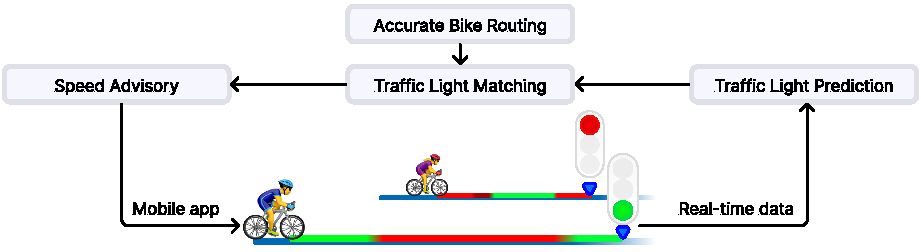
\includegraphics[width=\linewidth]{images/outline.png}
  \label{fig:outline}
\end{figure}

In \Cref{ch:prediction}, we will learn more about the different architectures for traffic light data infrastructures and how these impact speed advisory services. In particular, we will study prediction algorithms that provide a way for the app to look into the future and predict a signal's switching behavior and how this information is sent to the mobile app. The contribution of this work aims to understand Hamburg's system "Traffic Lights Data" (TLD) more thoroughly as a potential role model for other cities and critically review previous approaches.

After establishing a solid foundation and understanding of traffic light prediction, we will develop a solution in \Cref{ch:matching} that allows our app to match all signals along the user's trajectory. Unlike previous works, we will choose a new way of matching with a route-based approach. This will allow our app to easily predict the user's trajectory and efficiently match all signals in advance. As a bonus, the proposed system will circumvent any matching problems associated with inaccurate geolocation that impacted previous solutions.

In \Cref{ch:routing}, we will investigate how we can use Hamburg's reference maps for bike paths to provide a much more accurate routing than possible with open routing foundations. The idea is to utilize institutionally maintained routing foundations, so-called reference models, to provide consistent and accurate bike routing.

Up until this point, the discussions will mainly relate to the processes that must run in the backend of the GLOSA system. In \Cref{ch:app}, we will shift our perspective onto the mobile app with which real users will interact. We will look at various ideas to reduce distraction and enhance context-adaptiveness, including multiple different speed advisory user interfaces. As a product, we obtain a mobile application interleaved with a backend infrastructure implementing the concepts of this work.

With the obtained software infrastructure, we can roll out the application to users in Hamburg and run an extensive and realistic study. In \Cref{ch:impacts}, we will collect user telemetry and user feedback to look behind the scenes at how well the system works on a city scale. Various data analysis methods, including a calculation of the System Usability Score, will enable us to draw comparable results from the field test, which can be revisited in future studies that further improve upon the developed system.

\Cref{ch:conclusions} summarizes the gained knowledge and main results and gives an outlook for future studies. 

\chapter{Traffic Light Prediction}\label{ch:prediction}

 \section{Introduction}

The lack of awareness among road users about the planned switching of traffic lights leads to a series of well-known problems. Firstly, the issue of unneeded stopping and idling at red lights unnecessarily increases energy expenditure and emissions. In addition, not knowing about the upcoming traffic light's switching behavior also has negative impacts on road safety. There is a so-called dilemma zone when approaching a traffic light, where it unexpectedly turns yellow, and one must decide whether to stop before the light \cite{zhang_yellow_2014}. Often, this can lead to running a red light, speeding, or misunderstandings between drivers, increasing the overall risk of accidents.

Such situations exemplify where improved communication between vehicles and infrastructure elements could reduce the risk of accidents and the inefficiency of traffic. Collaborative awareness is a key driver in current research on Cooperative Intelligent Transport Systems (C-ITS). Predicting traffic lights and communicating this prediction to vehicles, establishing the C-ITS day-1 service GLOSA, is one integral part of a larger portfolio of potential measures \cite{mellegard_day_2020}. Nonetheless, it is important to consider that traffic light prediction is not strictly limited to GLOSA-like systems and may also lay the foundation for other application scenarios. Especially with the emergence of Augmented Reality, there may be many more application scenarios than we currently envision.

Despite these encouraging prospects, traffic light prediction is currently associated with multiple challenges. When intuitively considering the topic, one might assume that predicting the switching behavior of a traffic light should be straightforward based on its control program. In fact, the deployment of countdown displays at traffic lights based on these control programs is widespread, especially in Asian areas \cite{pan_impact_2023} and has recently also been studied for cyclists \cite{kaths_green_2019}. However, these countdown displays operate by transferring the residual phase time directly within the control unit to a countdown controller \cite{islam_improved_2016}. A mobile system would need to access this information from the outside.

Hence, a mobile system working across multiple intersections requires an interoperable data source. Here, the option exists to obtain the control programs directly, but without the current internal program state \cite{zweck_traffic_2013}. Since traffic-adaptive signals may only decide a few seconds before the next cycle how long the green phase will be switched \cite{islam_improved_2016}, this method is restricted to fixed-time traffic light control programs \cite{zweck_traffic_2013}. However, only 161 out of 1731 intersection nodes in Hamburg run a fixed-time program as of 2023. As seen in \Cref{tab:control-programs}, another factor hindering a prediction based on the engineering plans of control programs is the large variety of formats, in addition to the limited availability.

\begin{table}[htbp]
    \centering
    \begin{tabular}{lr}
        \hline
        \textbf{Control Method} & \textbf{\# Intersections} \\
        \hline
        \multicolumn{2}{l}{\textit{Adaptive Traffic Light Control Programs}} \\
        COMTESS* & 61 \\
        FLUSS* & 2 \\
        VS-PLUS* & 53 \\
        TELAN/TRENDS* & 14 \\
        Open Method of Traffic Control (OMTC) & 738  \\
        Switching based on request & 702 \\
        \hline
        \multicolumn{2}{l}{\textit{Non-Adaptive Traffic Light Control Programs}} \\
        Fixed-time (with audible signals for visually impaired people) & 69 \\
        Fixed-time (without audible signals for visually impaired people) & 92 \\
        \hline
        \multicolumn{2}{l}{\footnotesize{*: Gradually being replaced by OMTC.}}
    \end{tabular}
    \caption{Traffic control methods at intersections in Hamburg\footnotemark{}.}
    \label{tab:control-programs}
\end{table}

Due to these issues, another method for traffic light prediction has been established to deploy GLOSA-like applications in the field. Most GLOSA applications make use of the residual time provided by Signal Phase and Timing (SPaT) messages generated on the intersection controller level and transmitted to the vehicle. However, such messages may not always be available at the given location -- sometimes, as in this work, the prediction of traffic lights has to be performed purely by observing the outside state. In this chapter, we will discuss the various methods for obtaining traffic light state information and evaluate which methods are practical for cyclists.

One issue we will investigate in more detail is the traffic-adaptiveness of the switching programs. Traffic-adaptive adjustments of switching programs are intended to improve the traffic flow at an intersection but have adverse effects on predictability due to short-term green time adjustments. This means that a prediction based on historical data may not always be accurate to the second. Furthermore, a challenge when deploying a prediction algorithm is that traffic light data may not always arrive complete or on time, which is particularly problematic when the prediction needs to adapt quickly to a short-term change. Hence, tolerance for errors and robustness against missing information are also of high importance. If the prediction is unavailable or inaccurate, it can quickly lead to a loss of trust for the user or even become a safety risk.

\footnotetext{Source: Traffic control inventory of the LSBG / IVS1 (as of June 22, 2023) provided on request, in addition to an inquiry to the Hamburg senate. See \url{https://www.buergerschaft-hh.de/parldok/dokument/72143/ampelschaltsysteme_gruene_welle.pdf}}

The goals of this chapter are as follows. First, we will investigate potential sources of real-time traffic light data and evaluate their practicality for cyclist applications. Afterward, we will review approaches that address traffic-adaptive timing in traffic light predictions. Combining learnings from both domains, we establish methods for a traffic-light prediction infrastructure for Hamburg. Based on a broad analysis of the adaptivity seen in the real-time data, we will study at how many intersections a prediction could be challenging. This study allows us to draw conclusions about the suitability of our chosen prediction method. Finally, we evaluate the accuracy, availability, and scalability of the prediction algorithm over a time span of one year.

\section{Related Work}

Related work has been conducted on overcoming issues in obtaining traffic light data and predicting traffic lights based on that data. For data acquisition, decentralized and centralized systems have been proposed and studied. Largely independent of these studies, multiple prediction methods that aim to improve prediction accuracy have been proposed. However, a holistic approach to traffic light prediction requires interleaving both perspectives, considering that the prediction method is influenced by the technical constraints the data acquisition system imposes. Learnings from both domains must be joined to develop a state-of-the-art prediction system.

\subsection{Decentralized Systems}

In Europe, a large body of research and investments is flowing toward decentralized traffic light data systems, especially those based on Dedicated Short-Range Communication (DSRC). To operate these systems, Road Side Units (RSUs) are deployed at intersections where they send out standardized radio messages on the 5.9 GHz frequency band. These standardized C-ITS messages include SPaT messages, which vehicles can directly collect with a corresponding antenna (On Board Unit, OBU). An SPaT message contains not only the current switching state of a traffic light but also a residual time until the next switch, making it an ideal data foundation for GLOSA applications. Thus, many studies related to GLOSA utilize this data foundation \cite{schweiger_elisatm_2011, rakha_eco-driving_2011, rakha_aeris_2012, li_open_2012, suramardhana_driver-centric_2014, xu_bb_2015, bernais_design_2016, nguyen_efficient_2016, choudhury_integrated_2016, stahlmann_multi-hop_2017, stahlmann_exploring_2018, plianos_predictive_2018, zhang_green_2020, chen_developing_2022}.

SPaT messages are typically generated within the intersection controller level \cite{zweck_traffic_2013} and transmitted directly to an RSU without the need for a centralized server system. However, such a system is typically not fully decentralized. To calculate the residual time, there is the need for an additional prediction module, which may communicate with its own cloud in which a prediction algorithm is running \cite{strobl_c-its_2019, neuner_leitfaden_2020}. Due to the decentralized message transmission, however, a key advantage of this approach is that every vehicle equipped with a capable radio antenna has access to this data foundation. Thus, this approach is highly interoperable and attractive for manufacturers. The main per-unit cost factor resides in equipping intersections with the necessary RSUs \cite{niebel_cost-benefit-based_2013}.

A current research problem with decentralized approaches is the limited over-the-air radio transmission distance, especially when foliage blocks the line of sight. Since the 5.9 GHz frequency band resides closer to the visual light frequency spectrum of electromagnetic waves than other network carriers, such as 3G and 4G, it does not penetrate well through obstacles.  In response to this issue, the C-Roads project, a prominent initiative in Europe's C-ITS, submitted a statement advocating for the supplementation of the 5.9 GHz band with lower-frequency bands \cite{bohm_radio_2017}.

With DSRC only, Stahlmann et al. (2017) \cite{stahlmann_multi-hop_2017} show that the transmission range may be cut down by obstacles to less than 150 meters. The drop in the transmission rate is not immediate but gradual, which is why a partial message loss must always be assumed with this method. Sharara et al. (2019) \cite{sharara_impact_2019} provide more insights into the relation between packet loss, a GLOSA system's activation distance, and the speed advisory's effectiveness. The authors show that partial message loss up to 90\% is not a large problem unless the transmission distance is cut down too much, impacting the speed advisory system's activation distance and effectiveness. In a simulation with a specific green time of 25 seconds and red time of 40 seconds (amber = 5 seconds), Sharara et al. (2019) \cite{sharara_impact_2019} find that the transmission distance should be at least 850 meters for a 100\% success rate of traversing the green light, while 300 meters only resulted in 50\% -- 60\% of green passes depending on the message loss rate (90\% -- 10\%). Thus, with the transmission distance reported by Stahlmann et al. (2017) \cite{stahlmann_multi-hop_2017}, GLOSA applications may occasionally fall short of their potential benefit simply due to the transmission distance of the SPaT messages.

One explored solution to improve transmission range is an optimized RSU placement \cite{mehar_optimized_2015, massobrio_smart_2015, al-ezaly_optimal_2020}. Another option may be to adjust the transmission rate, which is reported in different ranges of 4 Hz \cite{stahlmann_multi-hop_2017} or 10 Hz in Hamburg \cite{stegen_ideas_2021}. The third option is inter-vehicle relaying of the messages to artificially expand the transmission range, as proposed by Stahlmann et al. (2017) \cite{stahlmann_multi-hop_2017}. Thus, a few practical solutions have already been presented that mitigate the problem of a limited transmission distance.

What has not been addressed so far is the system's compatibility with traffic participants who have no access to an inbuilt OBU. Although manufacturers Bosch\footnote{\url{https://www.bosch-presse.de/pressportal/de/en/auto-cycling-and-tech-innovators-launch-coalition-for-cyclist-safety-based-on-v2x-deployments-259136.html}} and Canyon\footnote{\url{https://media-centre.canyon.com/en-INT/226588-canyon-plan-to-integrate-autotalks-v2x-technology-into-bicycles-to-help-reduce-accidents}} may introduce OBUs into their bike components soon, currently, this approach is largely limited to cars, buses, trucks, and motorcycles. While the option of using a smartphone's inbuilt antenna array may exist, DSRC is incompatible with current smartphones \cite{jacob_ivs-kom_2020}. Even though external antennas are available, they require additional expenses by the user and come as roughly smartphone-sized devices \cite{kim_vulnerable_2017}\footnote{\url{https://auto-talks.com/products/zooz/}}. This makes such a solution unattractive for a standalone smartphone app.

One emerging alternative to 5.9 GHz radio is cellular V2X. This transmission technology utilizes an existing carrier medium such as 4G or 5G for the message transfer \cite{xia_field_2012, zweck_traffic_2013, bhattacharyya_assessing_2022}, distributing messages directly from an RSU (decentralized) \cite{bohm_radio_2017} or via cell towers (semi-decentralized) \cite{strobl_c-its_2019, jacob_ivs-kom_2020}. Although this carrier medium is interoperable on the application level (transmitting SPaT messages), its non-interoperability with DSRC \cite{bohm_radio_2017} on the network level leads to a displacement between both technologies. While DSRC is currently widely deployed on roads in Austria and Germany\footnote{\url{https://auto-talks.com/technology/dsrc-vs-c-v2x/}}, cellular V2X is seen by some stakeholders to potentially replace DSRC in the future\footnote{\label{cloudflight-article}\url{https://www.cloudflight.io/en/blog/5g-killer-app-v2x-requires-the-transformation-the-automotive-industry/}}. Amidst this uncertain state, C-ITS pilots \cite{strobl_c-its_2019} and OBU manufacturers \cite{jacob_ivs-kom_2020} develop multi-band solutions working with both cellular V2X and DSRC in parallel.

Another issue is the unclear long-term compatibility of cellular V2X with smartphones. Although chipsets exist that enable LTE-V2X through the PC5 mode (direct device-to-device communication) and LTE-V2X/5G-V2X via cell towers\footnote{\url{https://5gaa.org/content/uploads/2021/11/5GAA_List_of_C_V2X_devices.pdf}}, these chipsets are manufactured mainly for automotive applications. The 5G Automotive Association, a proponent of cellular V2X encompassing automotive manufacturers and chipset manufacturers, predicted LTE-V2X in 2017 to penetrate 80\% of new smartphones by 2027\footnote{\url{https://5gaa.org/content/uploads/2017/12/5GAA-Road-safety-FINAL2017-12-05.pdf}}. However, this prediction is based on an optimistic scenario in which smartphone manufacturers react to increasing demand for C-ITS applications induced by LTE-V2X deployments in cars. There is also the pessimistic scenario in which 0\% of smartphones will support this technology in the future. Currently, it is up for speculation which scenario is more likely, meaning that cellular V2X is also not yet an established data source for smartphone-based GLOSA applications.

\subsection{Centralized Systems}

While DSRC and cellular V2X have the goal of providing a near-range network for C-ITS message communication, there is also the option for a traditional approach over the Internet. With this approach, the traffic light data is collected at a centralized server infrastructure located near the traffic management center and redistributed over an internet endpoint \cite{zweck_traffic_2013, protschky_extensive_2014, protschky_adaptive_2014}. A centralized traffic light data infrastructure circumvents two challenges of decentralized approaches: limited transmission range and incompatibility with smartphones. However, it also shifts the responsibility of interoperability, data processing, and quality assurance toward the service consumer.

At Audi, Zweck et al. (2013) \cite{zweck_traffic_2013} established a data foundation that ingests traffic light data from three major cities. Correspondingly, three data adapters needed to be implemented: In Verona, the car manufacturer had access to SPaT messages generated on the intersection controller level. In Garmisch, each intersection controller needed to be retrofitted with an additional SWARCO forecast module to obtain the necessary data, presumably SPaT messages. In Berlin, multiple traffic control centers were connected with various protocols, for which the specific transmission format is not further disclosed. The implemented data adapters were integrated into a centralized proprietary backend of Audi, making the corresponding traffic light information available to the company's vehicles via a mobile network connection to the internet. Unfortunately, the specific prediction methods and challenges related to traffic light prediction are not provided in detail. The insights derived from this study and the potential knowledge gained are constrained by the lack of transparency in this regard. The available information indicates that the system was introduced in the United States in 2016 and is currently utilized to facilitate Audi's GLOSA services in Düsseldorf \cite{neuner_leitfaden_2020}.

Many studies, whether decentralized or centralized, utilize the contained prediction in SPaT messages directly to generate the GLOSA service without the need for an additional prediction system. In this way, these studies delegate the task of traffic light prediction to the infrastructure provider. However, some occasions may lead to the circumstance that the SPaT messages are not directly processable or available. The stability of the messages may also not be guaranteed at all times. As a result, an own prediction algorithm may be required that is not only scalable across multiple hundred intersection nodes, but also robust to data outages. This shows a study by Protschky et al. (2014) \cite{protschky_extensive_2014, protschky_adaptive_2014}. In this study conducted for BMW, the authors were confronted with a rather suboptimal data foundation in Munich. Usually, the delays in traffic light messages are within a few seconds \cite{neuner_leitfaden_2020}. However, in Munich, the authors had to work with SPaT messages arriving 10 to 60 minutes late as a result of the city's traffic light data infrastructure at the time. This meant that the residual prediction contained in the SPaT messages would be far outdated once the backend obtained this information. Furthermore, the traffic light messages did not only arrive late but also partially incomplete. Thus, the authors had to come up with some way to generate a prediction themselves. 

Protschky et al. (2014) \cite{protschky_extensive_2014, protschky_adaptive_2014} approached the challenges as follows. By recording the long-term history of a traffic light's actuation, the authors could generate a separate prediction decoupled from the real-time data, circumventing the message delays. Each generated prediction would contain a timeline between predicted "red" and "green" states after a given reference time. By incorporating a longer time frame of recorded traffic light states into the prediction algorithm, short-term losses and errors were statistically filtered out. Due to its computational simplicity, their approach is highly scalable. When detecting that the prediction would no longer correlate with the actual observed data to over 95\% accuracy, as required by BMW, the prediction was turned off for the affected traffic lights. As a result, the prediction availability would sometimes drop below 69\% while improving the overall trustworthiness of the existing predictions. Possible implications of this drop in availability on the users were not considered.

Compared to decentralized systems, centralized approaches to obtaining traffic light data are much more compatible with cyclist applications and still utilized today by at least one large car manufacturer. However, an ongoing challenge is to overcome the data issues of these systems. Protschky et al. (2014) \cite{protschky_extensive_2014, protschky_adaptive_2014} present an appealing solution that also applies to the data constraints in this work, in which no SPaT messages are available. Their approach only requires real-time information on traffic light colors and their cycle timing -- both are available in Hamburg through the centralized Traffic Light Data platform. Potential improvements of this solution include a more focused study of the data characteristics, the suitability of the chosen prediction algorithm, and the user's perspective. One particular issue is the reduced prediction availability in the presence of traffic-adaptive signal timing.

\subsection{Traffic-Adaptive Signal Timing}

The accuracy of predictions is negatively affected by shifted switching behavior as a result of traffic-adaptive traffic light timing intended to optimize the traffic flow. As noted by Otto et al. (2023) \cite{otto_framework_2023}, the dynamic shifting of traffic light timing reduces the effectivity and trustworthiness of the speed advisory. However, in which way the prediction is affected highly depends on the prediction algorithm. In general, there are two different approaches to prediction: self-adaptive prediction models and probabilistic prediction methods. Both respond differently to dynamics in traffic light behavior. Otto et al. (2023) \cite{otto_framework_2023} only refer to the traditional, probabilistic methods.

\begin{figure}[t]
\centering
\includegraphics[width=\linewidth]{images/prediction.pdf}
\caption{Probabilistic method of traffic light prediction with cycle stacking.}
\label{fig:prediction}
\end{figure}

Probabilistic methods have been proposed by Protschky et al. (2014) \cite{protschky_extensive_2014, protschky_adaptive_2014} and also Pape (2012) \cite{pape_untersuchung_2012}. The idea of these methods is as follows. Since a fixed per-traffic-light cycle length is mandatory even with fully adaptive traffic light programs \cite{protschky_extensive_2014}, the recorded history can be convolved into a stack of cycles as highlighted in \Cref{fig:prediction}. Then, the probability of "green" and "red" is determined for each second in the prediction vector depending on the prevalence of the predicted color at this specific second in previous cycles.

As discussed earlier, Protschky et al. (2014) \cite{protschky_extensive_2014, protschky_adaptive_2014} have shown that this method is not only scalable but also works well in the presence of high latencies or data losses of real-time traffic light messages. Since the adaptive component is represented as a probability, the speed advisory can focus on certain parts of the prediction, counteracting the adaptive behavior. To traffic adaptive signal timing, this kind of prediction algorithm reacts by blurring out certain parts of the prediction. Thus, as discussed by Otto et al. (2023) \cite{otto_framework_2023}, with a highly adaptive traffic light, one challenge is that the green and red predicted phases can become indistinguishable from each other. In case a target speed is calculated, the speed advisory algorithm must decide which parts of the prediction are considered safe enough. If no parts of the prediction exceed the defined certainty threshold, no speed advisory can be calculated. This is shown by Mahler et al. (2012) \cite{mahler_reducing_2012}, who developed an optimization method for calculating the optimal speed with an uncertain prediction. One challenge of this approach is that, as adaptability increases, it tends to converge more towards the midpoint of the green phase. Following the speed recommendation may result in the vehicle not reaching the traffic light precisely on time but rather with some delay.

Self-adaptive prediction models address this issue very differently. Through continually adapting the prediction to the observed real-time state, the prediction gets more accurate as it approaches the actual time of switching. Bodenheimer et al. (2014 -- 2015) \cite{bodenheimer_enabling_2014, bodenheimer_glosa_2015} were the first to propose such an approach through a graph-based method. This method observes the ingress directions at an intersection node and reconstructs the relation between the clearance timing of each direction. Schneegans et al. (2023) \cite{schneegans_prediction_2023} also demonstrate the possibility of utilizing machine learning models for this process. Here, the idea is to utilize a sequence prediction model trained on prerecorded timing data from a specific traffic light. Both models have the advantage that the predicted residual time readjusts toward the actual observed data at the expense of stretching or shortening the predicted residual time.

As Stahlmann et al. (2018) \cite{stahlmann_exploring_2018} point out, this stretching and shortening can also be seen as a major disadvantage of this approach. Since repeated adjustments to the prediction during the intersection approach negatively impact usability, there is a clear tradeoff between the prediction's accuracy and temporal stability. The increased computational complexity of the presented models is also a factor that may negatively impact the prediction algorithm's scalability toward multiple thousand signals. There is currently no evidence supporting the scalability on a large scale as opposed to probabilistic approaches \cite{protschky_extensive_2014, protschky_adaptive_2014}. Furthermore, while the probabilistic approach is intrinsically robust to incomplete data and can drop individual cycles, error robustness is another factor to consider in the evaluation of self-adaptive models. These challenges must be addressed in order to employ such a model in practice. Most importantly, however, the traffic light data must arrive in time for the self-adaption to happen. Thus, self-adaptive prediction methods can only be employed when the traffic light data arrives with a low latency. In a situation such as reported by Protschky et al. (2014) \cite{protschky_extensive_2014, protschky_adaptive_2014} where traffic light messages may arrive with a delay of over 10 minutes, such models are likely not a good option.

To resolve the dispute between probabilistic and self-adaptive methods, an overarching question is how many traffic lights are, in fact, traffic-adaptive and to what extent they are adaptive. This question must be answered to determine the likelihood that users will encounter inaccurate predictions at intersections. Looking at related work, various studies report different levels of adaptiveness. Cai et al. (2009) \cite{cai_adaptive_2009} were the first to report that "most" signals in their context are traffic-adaptive. Concrete numbers were presented by Bodenheimer et al. (2014) \cite{bodenheimer_enabling_2014}, who reported that 95\% of signals in Hamburg are adaptive, with 73\% being fully or semi-adaptive in the ten largest German cities. Fakler et al. (2014) \cite{fakler_structures_2014} also found a high proportion of traffic-actuated control systems in German cities with over 50,000 inhabitants. Schneegans et al. (2022) \cite{scheegans_exploiting_2022} and Heckmann et al. (2023) \cite{heckmann_stage_2023} further support the conclusion that most traffic lights are operated by traffic-adaptive controls. Hao et al. (2019) \cite{hao_eco-approach_2019} noted the widespread deployment of actuated traffic light controllers in the US, while Avatefipour and Sadry (2019) \cite{avatefipour_traffic_2018} found that fixed timing is more prevalent in Malaysia. Grumert and Pereira (2022) \cite{grumert_heads-up_2022} observed that 70\% of signals in Sweden are adaptive. However, there are also contradictory statements, such as Olaverri-Monreal et al. (2018) \cite{olaverri-monreal_implementation_2018} reporting that adaptive timing is only implemented in a small number of road networks, and the majority of urban areas still use pre-timed control systems.

It must be considered that the reported proportions of adaptive traffic lights are often not verifiable through external sources. For example, in a work by Bodenheimer et al. (2014) \cite{bodenheimer_enabling_2014}, which mentions 95\% adaptive traffic lights, it was only clarified upon inquiry that these results were based on a survey conducted by a service provider on behalf of Audi. Nonetheless, the main findings seem to align with the distribution reported by Hamburg's authorities, which lies at 90.7\% (1570 from 1731) of control programs capable of traffic-adaptiveness. However, this does not necessarily mean that all 90.7\% of adaptive traffic lights also express adaptive switching behavior. In theory, the capability can be unused or only expressed in minor shifts, which would result in a less problematic impact on the prediction, as suggested by the reported percentages.

\begin{Summary}[Summary of Research Gap]
Many works focus on decentralized data transmission, which is currently not available for cyclist applications. At the moment, cyclist applications of traffic light information services require a centralized traffic light data platform. Most centralized platforms appear to retransmit SPaT messages generated at the intersection controller level. Here, the residual time prediction in SPaT messages can be directly used for a speed advisory application. However, in some cases, SPaT messages may not be available or arrive too late, requiring an own prediction method. Using a probabilistic prediction method seems to be a promising option to implement the traffic light prediction. This approach has already proven effective in the context of centralized systems, as opposed to self-adaptive prediction methods. Whether self-adaptive models can contribute to an enhanced traffic light prediction is subject to the completeness and recency of traffic light data, but also the tradeoff between temporal stability and prediction accuracy. To study this relation further, a direct analysis of traffic light data is required to determine how many traffic lights actually exhibit dynamic behavior and the extent of their dynamism. However, such a study has not yet been conducted. Conclusions regarding the extent to which the dynamism of traffic lights may pose a motivation for self-adaptive prediction systems are, therefore, not definitively established. This constitutes an important research gap.
\end{Summary}

\section{Concept}\label{sec:signal-prediction}

We will conduct two steps to address the described research gaps. First, we will design a prediction infrastructure with the available data foundations in Hamburg. Specifically, we will focus on the chain of information from the traffic lights to the cyclist and identify issues in the data transmission that require further consideration. Since our data infrastructure will also be bound to delays and losses in the traffic light messages, we will use the prediction method proposed by Pape (2012) \cite{pape_untersuchung_2012} and Protschky et al. (2014) \cite{protschky_extensive_2014, protschky_adaptive_2014} that is designed to be robust against these issues. This prediction method should adapt to practically all centralized traffic light data infrastructures discussed in the available literature. It is also compatible if no SPaT messages are available since it only requires the traffic light's colors and cycle time information, which can also be delayed. Finally, we analyze how suitable the prediction algorithm is for our scenario based on the large-scale evaluation of the traffic light data. Here, we will focus on the adaptivity of traffic lights and the consequences of these on the prediction's usability.

\subsection{Prediction Infrastructure}

As discussed in the related work section, providing a traffic light prediction service for users of a cyclist application is strongly linked to the ability to obtain the corresponding real-time data. Although Hamburg provides RSUs at intersections that send SPaT messages, this data source is excluded from further consideration due to its current incompatibility with a smartphone application. Utilizing the control program engineering plans directly to obtain a prediction is also not an option for 90.7\% of the traffic lights in Hamburg. Fortunately, Hamburg provides a centralized traffic light data broker service, the Traffic Light Data (TLD) platform, that provides the necessary real-time data. This platform will be considered the foundation for this work.

\begin{figure}[t]
\centering
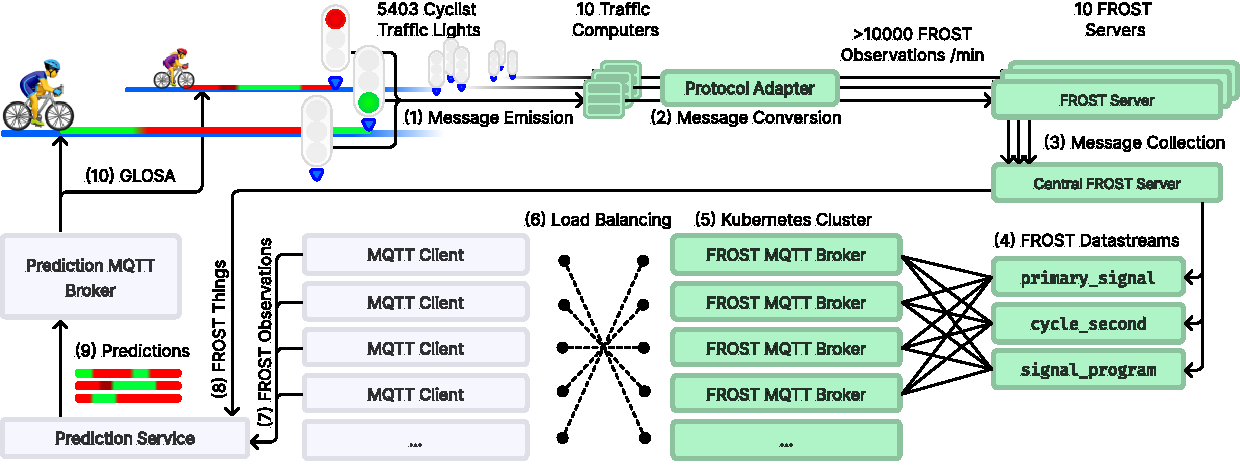
\includegraphics[width=\linewidth]{images/traffic-light-data-infrastructure.pdf}
\caption{Designed traffic light data adapter for Hamburg's Traffic Lights Data platform.}
\label{fig:traffic-light-data-infrastructure}
\end{figure}

It is crucial to understand the type of information provided by the centralized data broker. As mentioned previously, the Traffic Light Data broker does not directly provide SPaT messages, and also no residual time until the next phase change. Instead, the traffic light state messages are provided as observations of the external traffic light state. Specifically, the state messages are provided in the OGC SensorThings\footnote{\url{https://www.ogc.org/standard/sensorthings/}} "Observation" format. Each time the signal changes its color, switches to another program, or restarts a cycle, an Observation is generated and distributed on a corresponding information channel via an MQTT broker. The prediction algorithm has to ingest this data and generate a prediction of the future states.

Until the traffic light state messages arrive at the prediction service, they are translated and shifted multiple times between various data brokers. \Cref{fig:traffic-light-data-infrastructure} highlights Hamburg's data pipeline. First, the state messages are sent in a controller-specific format, such as OCIT\footnote{\url{https://www.ocit.org/de/ocit/schnittstellen/}}, to one of ten traffic computers (1). Then, the messages are converted to Observations (2) and sent to a corresponding SensorThings server. From there, a centralized SensorThings server collects all Observations (3), which are associated with a specific type of "Datastream" encapsulating the type of Observation: \texttt{primary\_signal} for traffic light color, \texttt{cycle\_second} for cycle timing, and \texttt{signal\_program} for program change (4). Finally, the messages are redistributed across an autoscaled cluster of SensorThings MQTT brokers (5). 

From there, the prediction service connects to the broker endpoint to ingest all Observation messages. To reduce the load on each individual MQTT broker, the prediction service utilizes multiple MQTT clients with individual TCP connections (6). The collected Observations (7) are combined, knowing which Observation is associated with which Datastream and which traffic light is represented by a "Thing" (8). This allows the prediction service to record the traffic light history and employ the probabilistic prediction method proposed by Pape (2012) \cite{pape_untersuchung_2012} and Protschky et al. (2014) \cite{protschky_extensive_2014, protschky_adaptive_2014} (9). Every 60 seconds, a new prediction of 180 seconds into the future is generated for each traffic light and distributed to the smartphone app via MQTT (10). Each smartphone app is subscribed to the MQTT topic of the upcoming traffic light, meaning that predictions are automatically updated on the client side.

\begin{figure}[t]
\centering
\includegraphics[width=\linewidth]{images/monitoring-screenshot.png}
\caption{Screenshot of the developed monitoring solution. The dashboard displays the current spatial availability and quality of predictions, as well as a timeline for the ingress data and the prediction quality.}
\label{fig:monitoring-screenshot}
\end{figure}

Each time a state message is shifted along the presented chain of information, it introduces a delay and a possible point of failure. As a consequence, the prediction service must be robust against delayed or missing state messages. However, these issues are not evenly distributed across all traffic lights. They may arise in specific areas in the city or from time to time. Thus, it is also important to monitor this behavior and identify and address systematic issues in the traffic light data infrastructure. As a foundation, as shown in \Cref{fig:monitoring-screenshot}, a monitoring system was implemented that highlights data outages across the city and along a timeline.

In addition to these coarse-grained methods, another error-detection is implemented that detects missing state messages for traffic lights. The designed detection makes use of the shifting pattern red-redamber-green-amber and red-green. Transitions between phases are checked against these allowed transitions. If an illegal transition occurs, the currently recorded cycle is discarded. This makes use of the probabilistic prediction method's robustness against missing cycles.

\begin{figure}[htbp]
\centering
\includegraphics[width=\linewidth]{images/home-view-prediction-quality.png}
\caption{Prediction quality visualized in the GLOSA app for enhanced explainability.}
\label{fig:home-view-prediction-quality}
\end{figure}

Not all traffic lights in Hamburg are available for prediction. Those who are available may occasionally lose data, which error detection can partially address. Another important factor, however, is the user's perspective on the data availability. Since a degraded prediction availability will also negatively impact usability, some ideas must be found that mitigate potential disappointments on the user side. One idea implemented in the GLOSA app is increasing the explainability of the prediction system. The existing monitoring infrastructure is extended such that users can also access information about the current availability. Through the app, users can inform themselves about the current percentage of available predictions and the spatial distribution of good and bad predictions on the map. The resulting user interface shown in \Cref{fig:home-view-prediction-quality} is intended to allow users to identify faults at an early stage and then switch to an alternative app, avoiding frustration caused by missing or incorrect predictions.

\subsection{Adaptivity Analysis} 

The chosen probabilistic prediction method assumes that the green phases should roughly align with each other across the recorded cycles. Depending on the specific traffic light control program, the traffic light's deviation from a recurring base pattern may be more or less influenced by incoming traffic. Although it is clear that, as of 2023, 90.7\% of traffic lights in Hamburg \textit{can} adapt to inbound traffic, it is unclear how pronounced this behavior is. To fill this knowledge gap, we can directly measure the traffic adaptivity based on the same data provided by the SensorThings API in Hamburg. The collected information can then be utilized to estimate how well the probabilistic method will predict the traffic lights and how it may perform in relation to other methods.

First, it must be determined which metrics are suitable for measuring characteristics of traffic adaptivity. One aspect of traffic adaptivity that can be directly measured from the recorded cycles is the shift of the green phase. We can measure the green phase's start time $g_{start}(L_j)$ and end time $g_{end}(L_j)$ in each cycle $L_j$, and calculate the shift between both:

\[ \text{Shift}(L_1, L_2) = [g_{start}(L_2) - g_{start}(L_1), g_{end}(L_2) - g_{end}(L_1)] \]

In the example given in \Cref{fig:types-of-adaptiveness}, $\text{Shift}$$(L_1, L_2)$ would be $[-2, -2]$ and $\text{Shift}$$(L_2, L_3) $$= [3, 3]$. While partially adaptive traffic lights, as highlighted in \Cref{fig:types-of-adaptiveness} are assumed to shift the green phase within the cycle, other traffic lights may only insert a green phase once a vehicle is detected. Thus, one problem of this metric is that each cycle may have different numbers of green phases. As a result, we have to discard additional green phases at the end of one cycle that are not seen in the other cycle, potentially leading to some discarded information. 

\begin{figure}[t]
    \centering
    \includegraphics[width=0.75\linewidth]{images/explanation-partially-adaptive.pdf}
    \caption{Partially adaptive traffic light switching pattern as highlighted by Otto et al. (2023) \cite{otto_framework_2023}}\label{fig:types-of-adaptiveness}
\end{figure}

To account for this loss of information, we calculate another metric to capture the cycles that are not fully considered through the Shift metric. This metric indirectly measures the deviation by the number of seconds in the current cycle that deviate from the previous cycle. We name this metric "Distance" since it calculates the second-wise distance between the cycles. The Distance metric between two cycles $L_1$ and $L_2$, with the lengths $l_1$ and $l_2$ calculated as follows:

\[ \text{Distance}(L_1, L_2) =  \sum_{i=0}^{\max(l_1, l_2)-1} \left\{
\begin{array}{ll}
1 & \text{if } i \geq l_1 \text{ or } i \geq l_2 \\
1 & \text{if } L_1[i] \neq L_2[i] \\
0 & \text{otherwise}
\end{array} \right.\]

If we apply this metric to the example in \Cref{fig:types-of-adaptiveness}, we get $\text{Distance}$$(L_1, L_2)$$ = 4$ and $\text{Distance}$$(L_2, L_3)$$ = 6$. This metric captures all second-wise differences but not the directionality of the green phase shifts. This means that traffic lights expressing a "staircase" pattern, in which the green phase is shifted by a constantly increasing factor each cycle, will be measured as highly adaptive, although they express a relatively predictable pattern. As a consequence, both the Distance and Shift metrics are used in conjunction with the recorded traffic light data.

\begin{Summary}[Summary of Methods]
The designed prediction infrastructure makes use of Hamburg's centralized Traffic Light Data platform and reuses the existing probabilistic prediction method  \cite{pape_untersuchung_2012, protschky_extensive_2014, protschky_adaptive_2014} guaranteeing scalability in addition to robustness to latencies and data errors. Interoperability with platforms without the availability of intersection-controller-level predictions (as with SPaT messages) is also given since the prediction algorithm only relies on the availability of traffic light colors and cycle timing information. Additional measures are implemented that detect and discard erroneous data. Through a monitoring system the prediction quality can be analyzed and systematic issues identified. Information about the prediction availability is forwarded to the user to enhance the explainability of outages. In addition to this monitoring system, an adaptivity analysis is conducted to explore the traffic-adaptiveness of traffic lights. This adaptivity analysis reuses the traffic light data infrastructure for direct measurement of the adaptiveness instead of extrapolating on the reported number of 90.7\% adaptive traffic lights. The adaptiveness is measured with two metrics in conjunction: the Distance metric incorporating the absolute shift between traffic light cycles, and the Shift metric that measures the directionality in the traffic light switching patterns.
\end{Summary}

\section{Results}

- Die Evaluation der Prognoseinfrastruktur ist zweigeteilt: die Auswertung des Prognoseverfahrens und die Auswertung der Verkehrsadaptivität von Ampeln in Hamburg.

- Als erstes betrachten wir, wie gut das Prognosesystem im Zusammenspiel mit der Hamburger Ampeldatenplattform funktioniert, und wo mögliche Schwachstellen sind.
- Dazu schauen wir uns die räumliche Abdeckung und den Verlauf der Ampelprognosen über einen längern Zeitraum an. Die Grundlage dafür bilden die Aufgezeichneten Metriken des umgesetzten Monitoring-Systems
- Wir schauen uns den zeitlichen Verlauf der Prognoseverfügbarkeit an. Dies gibt uns Aufschlüsse darüber, an wievielen Ampeln in Hamburg Geschwindigkeitsempfehlungen zu erwarten sind, und dass dies deutlich weniger sind als gewünscht
- Um genauer nachzuvollziehen, warum die Prognoseverfügbarkeit niedriger als gewünscht ist, schauen wir auf die aufgezeichneten Metriken des umgesetzten Monitoring-Tools
- Wir identifizieren bestimmte wiederkehrende Fehlermuster, die auf systematische Fehler in der Hamburger Dateninfrastruktur hinweisen
- Gemeinsam mit den Betreibern der Datenplattform ziehen wir Rückschlüsse auf die Problemursachen und beschreiben mögliche Lösungsansätze
- Um die Skalierbarkeit des Prognosealgorithmus nochmals zu zeigen schauen wir uns noch kurz die CPU, RAM und Netzwerkauslastung des Prognosedienstes an

- Der zweite Teil der Evaluation bezieht sich auf die Untersuchung der Verkehrsadaptivität über die Echtzeitdaten
- Wir betrachten den Tag-Nacht Zyklus der Verkehrsabhängigkeit von Wochentag zu Wochentag und schauen uns an, wie stark die Grünphase der Ampeln in einem Zyklus nach vorn und hinten schwankt. Grundlage hierfür ist die entwickelte Distance metrik
- Außerdem schauen wir uns an, ob die Grünphasen tendenziell gleichverteilt innerhalb des Zyklus nach vorn oder hinten streuen, oder ob es Ampeln mit Stufenmustern gibt, bei denen die Grünphase nur nach vorn oder nur nach hinten streut
- Anhand einer Karte betrachten wir, ob die Verkehrsabhängigkeit wie erwartet immer ganze Knoten mit mehreren Ampeln betrifft, oder auch einzelne Ampeln
- Diese drei Analysen helfen uns, genauer einzuschätzen, an wie vielen Kreuzungen das gestaltete Prognoseverfahren geeignet ist

\subsection{Long-Term Study of Prediction Availability, Quality, and Scalability}

\begin{table}[b]
    \centering
    \begin{tabular}{@{}l|ccccccccc|r@{}}
        \hline
        Lane type & \multicolumn{9}{c|}{Tag according to \texttt{Thing/properties/laneType}} & $\Sigma$ \\
        \hline
        Car        & $\blacksquare$ & $\blacksquare$ & $\blacksquare$ &   &   & $\blacksquare$ &   &   &   &  9649 \\
        Bus        &   &   & $\blacksquare$ &   &   & $\blacksquare$ & $\blacksquare$ &   & $\blacksquare$ &  1309 \\
        Bike     & $\blacksquare$ &   & $\blacksquare$ & $\blacksquare$ &   &   &   & $\blacksquare$ & $\blacksquare$ &  5477 \\
        Pedestrian &   &   &   &   & $\blacksquare$ &   &   & $\blacksquare$ &   &  6408 \\
        \hline
        $\Sigma$ (unique) & 1509 & 7077 & 217 & 3646 & 6315 & 846 & 234 & 93 & 12 & \\
        \hline
    \end{tabular}
    \caption{Number of individual traffic lights (connections) in the Traffic Lights Data platform, as of Dec 4, 2023.}
    \label{tab:tld-number-of-things}
\end{table}

- Bei der Betrachtung des zeitlichen Verlauf der Prognose muss zunächst beachtet werden: Die Anzahl Ampeln in der Traffic Lights Data plattform nimmt stetig zu
- Wir können die ID der individuellen Ampeln (connections) nutzen um die Anzahl Kreuzungen zu bestimmen, wie z.B. \texttt{353\_12} für Kreuzungsknoten 353 und Connection 12
- Siehe \Cref{tab:tld-number-of-things}: Zum Stand Dezember 2023 befanden sich 19951 ampeln (connections) verteilt über 791 kreuzungsknoten im System. Dies ergibt eine Abdeckung von 45.7\% (von 1731) der signalisierten Kreuzungen
- Bei der Sichtung der Ampeln wurden zwei kleine Fehler festgestellt:
- Bei einer der Ampeln (132\_22) wurde ein doppelter cycle\_second Datastream festgestellt
- Außerdem wurden bei den 2 Connections 240\_1 und 240\_2 fälschlicherweise der laneType "16371" angegeben, der eigentlich die Meldepunktnummer darstellt. Diese sind in \Cref{tab:tld-number-of-things} nicht mit aufgeführt, da sie nicht zugeordnet werden können
- Beide Probleme konnten durch Kommunikation mit den Betreibern auf Fehler in der Dateneinpflegung zurückgeführt werden. Die Behebung der Fehler wurde eingeleitet.

- Stand Dec 4, 2023 sind von den 19951 Ampeln 5477 für die Benutzung durch Radfahrer markiert und damit relevant für unser bike-GLOSA System. Auch eine Mischbenutzung durch ÖPNV, Fußgänger, und Autos zusammen mit Fahrrädern ist hierbei mit einbezogen
- Die aufgezeichneten Daten für diese Ampeln ergeben, gemessen über einen Zeitraum von 365 Tagen (Dec 4, 2022 -- Dec 4, 2023), im Durchschnitt 8532 primary\_signal Observations, 3318 cycle\_second Observations, und 27.7 program\_change Observations pro Minute die über MQTT empfangen und verarbeitet werden
- In dieser Zeit war der Prediction Service 75h wegen geplanten Wartungsarbeiten oder technischen Problemen offline und 8680h online (99.14\% uptime). Für 5h ist der Status unklar, da die gesamte VM oder nur das Monitoring offline war. Mit 80h angenommer Downtime kommen wir auf 99.08\% uptime. Daher sollte beachtet werden, wenn die nachfolgenden Metriken interpretiert werden, dass nicht 100\% des Zeitraums abgedeckt sind

\begin{figure}[t]
    \centering
    \includegraphics[width=\linewidth]{images/monitoring-availability.pdf}
    \caption{Long-term development of prediction availability.}\label{fig:monitoring-availability}
\end{figure}

- Den Langzeit-Datenverlauf sowie die Prognoseverfügbarkeit ist in  \Cref{fig:monitoring-availability} gezeigt.
- Die Prognoseverfügbarkeit errechnet sich hierbei einfach aus der Anzahl Prognosen für Ampeln, die minütlich vom Prognosedienst erzeugt werden, durch die Anzahl verfügbarer Connections
- Im oberen Teil der Abbildung sehen wir, dass die Prognoseverfügbarkeit sich im Normalfall zwischen 40\% und 80\% bewegt. 100\% werden nie erreicht.
- Die Prognoseverfügbarkeit schwankt im Tagesverlauf, aber auch im längeren Verlauf der Aufzeichnung
- Betrachten wir den längeren Verlauf, sehen wir, dass nach einer initialen Zeit mit relativ stabiler Prognoseverfügbarkeit im Sommer 2023 vermehrt Einbrüche zu beobachten sind. Diese stabilisieren sich gegen Oktober 2023 wieder, kommen aber nicht wieder auf das Niveau vom Frühjahr 2023.
- Die Einbrüche im Sommer 2023 sind hauptsächlich dadurch zu erklären, dass während dieser Zeit vermehrt Wartungsarbeiten am Traffic Lights Data System stattfanden. Es wurden wiederholt Updates durchgeführt, die zu einer Verschlechterung der Datensituation führten

- An den Tagen um den 11. Juli 2023 (1) kam es beispielsweise zu dem Problem, dass alle Observations doppelt geschickt wurden. Dies hatte zur Folge, dass die Prognoseverfügbarkeit für diesen Zeitraum fast auf 0\% zurück ging. Dies ist bisher der größte beobachtete Einbruch. Eine Vermutung, warum hierbei die Prognoseverfügbarkeit so stark einbrach, ist, dass die Duplikate der Nachrichten von einem gespiegelten System mit anderer Latenz kamen, und somit zu einer unterschiedlichen Zeit als die originale eintrafen.
- An den Tagen um den 23. November 2023 (2) wurde ein Feature für den Prognosedienst getestet, welches nicht funktionierende Ampeln aus dem System ausschließt. Daher ist die relative Verfügbarkeit in dieser Zeit kurz gestiegen trotz fallender Anzahl von Observations. 
- Abgesehen von diesen zwei besonderen Situationen ist aber klar sichtbar, dass die Prognoseverfügbarkeit stark mit der absoluten Anzahl der Nachrichten korelliert
- Ebenfalls ungeklärt ist der Abfall der signal\_program observations im Dezember 2022. Ob zum jetzigen Zeitpunkt nur ein Bruchteil der eigentlichen Programm-Observations kommen, oder im Dezember 2022 zu viele dieser Observations gesendet wurden, kann mangels einer Ground-Truth und einer Aufzeichnung genauerer Metriken für diesen Zeitraum nicht nachvollzogen werden

- Was bei der Betrachtung der Prognoseverfügbarkeit in \Cref{fig:monitoring-availability} nicht eingerechnet ist, ist die Qualität der Prognose. 
- Ein Teil der Prognosen wird zwar erstellt, hat jedoch eine niedrige Qualität. Da bei einer Prognosequalität niedriger als 50\% keine Geschwindigkeitsempfehlung dargestellt wird, ist die tatsächliche Verfügbarkeit von Geschwindigkeitsempfehlungen immer niedriger als die Prognoseverfügbarkeit

\begin{figure}[t]
    \centering
    \includegraphics[width=\linewidth]{images/monitoring-long-term-study.pdf}
    \caption{Long-term development of prediction quality.}\label{fig:monitoring-long-term-study}
\end{figure}

- Die Qualität der Prognosen ist in \Cref{fig:monitoring-long-term-study} genauer dargestellt
- Die Messung der Qualität findet statt durch einen kontinuierlichen Vergleich der Prognose mit den tatsächlich eingehenden Daten
- Stimmen alle Sekunden in der Prognose mit den aktuellen Daten überein, so errechnet sich eine Prognosequalität von 100\%. Stimmt keine Sekunde überein, so ergibt dies 0\% Prognosequalität. In der aktuellen Implementation des Prognoseverfahrens gibt es noch die Prognosequalität -1, die dann erzeugt wird, wenn nicht mindestens 5 Zyklen in den letzten 30 Minuten zur Validierung vorliegen. In \Cref{fig:monitoring-long-term-study} wird dies als Prognose mit Qualität 0\% gemapped 
- Im Langzeitverlauf sieht man zunächst einen ähnlichen Verlauf bei der Prognoseverfügbarkeit 100\% im Vergleich zu \Cref{fig:monitoring-availability} - sehr prägnant ist hier auch der Einbruch rund um den 11. Juli 2023 durch die duplizierten Observations, sowie die generell über den Jahresverlauf 2023 eingebrochene Verfügbarkeit

- Weiterhin sieht man, dass die Prognosequalität sehr zweigespalten ist: nur wenige Prognosen liegen im Bereich 10\% -- 90\% Qualität - wenn man die Prognosequalität als Genauigkeitsmetrik interpretiert, scheinen die meisten Prognosen also auf wenige Sekunden genau zu sein
- Was man jedoch auch sieht sind die vermehrten Prognosen bei 0\% Qualität Seit ca. Juli 2023. 
- Da der Prognosealgorithmus nur dann eine Prognose erzeugt, wenn bereits zu einem früheren Zeitpunkt Echtzeitdaten der Ampel vorhanden waren, lässt dies auf zwischenzeitliche Datenausfälle schließen
- Diese Datenausfälle können normal sein, beispielsweise bei der nächtlichen Abschaltung einer Ampel, oder auch nicht gewollt, wenn dies außerplanmäßig und irregular geschieht. Letzteres würde dann auf ein systematisches Problem in der Dateninfrastruktur hindeuten
- Also lohnt es sich, nochmal einen genaueren Blick auf die Datenausfälle zu richten

\begin{figure}[htbp]
    \centering
    \begin{tabular}{@{}cp{5cm}c@{}}
    (a) 6:00 UTC & & (b) 7:00 UTC\\
    \end{tabular}
    \includegraphics[width=\linewidth]{images/monitoring-before-after-failure.png}
    \caption{Before and after traffic computer failure on Oct 11, 2023. Green to red: 100\% to 0\% prediction quality. Black: no prediction, or quality -1.}\label{fig:monitoring-failure}
\end{figure}

- Ein willkürlich gewähltes Beispiel eines solchen Datenausfalls ist in \Cref{fig:monitoring-failure} gezeigt.
- Sichtbar sind hierbei zwei Arten von Problemen: Ausfälle vereinzelter Ampeln (links und rechts) und Ausfälle ganzer Stadtteile (nur rechts)
- Bei Ausfällen einzelner Ampeln 

- TEST wird dies synchronisiert?

\begin{figure}[htbp]
    \centering
    \includegraphics[width=\linewidth]{images/monitoring-failure.pdf}
    \caption{Monitored metrics during traffic computer failure on Oct 11, 2023.}\label{fig:monitoring-failure}
\end{figure}

\begin{figure}[htbp]
    \centering
    \includegraphics[width=\linewidth]{images/monitoring-7-days.pdf}
    \caption{Reoccurring traffic computer failures after 6:00 UTC.}\label{fig:monitoring-7-days}
\end{figure}

Together with the Traffic Light Data system operators (LSBG, HHVA, SWARCO), this monitoring system was utilized to identify multiple problems:

\begin{enumerate}
    \item It occasionally happens that traffic control centers need to undergo maintenance. During this period, real-time data is usually not available for a particular area of the city.
    \item During the day, the SensorThings brokers cannot keep up with the incoming number of messages. Consequently, brokers' queues fill up, leading to dropped messages.
    \item Messages from specific traffic control centers can arrive with significant delays of several minutes. This may prevent the generation of predictions for certain traffic lights, as the constraint for time criticality is violated.
    \item Some traffic lights were connected to the Traffic Lights Data platform, although their protocol is currently not supported by the protocol adapter. These traffic lights would be offline all the time.
    \item Due to construction or general changes in intersection layouts, some traffic lights would be associated with the wrong ID or not exist anymore.
\end{enumerate}

Based on the collected knowledge, these issues could be addressed accordingly. First, the platform operators were able to improve the stability of affected brokers. Then, to address issues 3--5, all traffic nodes associated with the erroneous traffic computers and erroneous traffic lights were excluded based on a list provided by the system's operators. This significantly reduces the number of available traffic lights for the prediction system but ensures that predictions are only provided for functional traffic lights.

Lösungsmöglichkeiten:
- HTTP-MQTT-Syncing (für Datenaufzeichnung zu Evaluationsteil 2 verwendet, aber für Datenaufzeichnung des Prognosesystems nicht)

- To show the effect of the improvements: rejected cycles metric

\begin{figure}
    \centering
    \includegraphics[width=\linewidth]{images/monitoring-rejected-cycles.pdf}
    \caption{Cycles rejected due to out-of-order phase sequence.}\label{fig:monitoring-rejected-cycles}
\end{figure}

\begin{figure}
    \centering
    \includegraphics[width=\linewidth]{images/monitoring-prediction-service-load.pdf}
    \caption{Cadvisor statistics for prediction service.}\label{fig:monitoring-prediction-service-load}
\end{figure}



\subsection{Study of Traffic-Adaptivity in Hamburg}

...

\section{Conclusions}

\chapter{Traffic Light Matching}\label{ch:matching}

\begin{Summary}[Bibliographical Notes]
This chapter is based on the following two papers in which the author was the principal investigator: 

\cite{matthes2022matching} \fullcite{matthes2022matching}

\cite{matthes2023geo} \fullcite{matthes2023geo}
\end{Summary}

\section{Introduction}

Accurately detecting upcoming traffic lights is crucial for many driving applications. It is not only a safety-critical functionality for (semi)autonomous driving systems but is also essential for bridging the gap between traffic light prediction and speed recommendation. So far, we have considered the traffic light prediction without its relationship to the traffic light's position along the user's trajectory. However, to determine the relevant traffic lights along the user's pathway, we must not only know about the predicted timing of the traffic light but also about its position and whether it aligns with the predicted path. A georeferencing is required.

The concept of georeferencing intersections, initially proposed under the name Geometric Intersection Description (GID), was introduced relatively early in the USA in 2008 \cite{cicas-v}. To not only reference the position of traffic lights, but also the specific turns served by them, the turn lane shapes are represented as line geometries crossing the intersection. In this way, it is possible to distinguish between turn directions and find which specific traffic light will be relevant for the vehicle. Today, this information is represented in the internationally standardized MapData (MAP) format that was developed by the SAE\footnote{\url{https://www.sae.org/standards/content/j2735_202309/}} in coevolution with the Signal Phase and Timing (SPaT) message standard.

MAPs, like SPaTs, can reach the road user through various channels, encountering similar transmission issues as SPaTs (see \Cref{ch:prediction}). However, since MAPs are less frequently updated, collecting, transferring to a database, and redistributing the lane geometries is possible. This makes it viable to maintain a centralized directory service in which each lane is mapped. In Hamburg, this centralized directory service is provided by the Traffic Lights Data platform that takes its information from the MAPs developed by engineering bureaus for Hamburg's intersections.

A more significant challenge than the acquisition of intersection topologies is determining which lane on the intersection will be used by a road user approaching it. Typically, there are multiple individual paths that can be chosen when crossing an intersection, and the concrete choice may depend on the user's route, mode of transportation, situation, or general preference. Due to the complexity of real-world traffic, a sudden lane change to align with the traffic perceived as the best option is possible, requiring the system to adapt quickly to the new lane or anticipate the direction in which the user wants to travel. 

While cars are usually restricted by a few available lanes, cyclists or pedestrians often have multiple ambiguous options to cross an intersection. Moreover, cyclists or pedestrians may approach a traffic light from several directions, leading to no clear entry lane. This leads to the issue that the user's position cannot simply be matched to the nearest entry lane's geometry. Therefore, the problem of matching the correct traffic lights is highly complex, and even more so for cyclist applications.

This chapter aims to address this problem and develop a practical solution for cyclist traffic light matching. First, we review related work and how they address the problem, identifying three core approaches: vision-based using cameras or similar sensors for traffic light identification, location-based using global navigation and satellite systems (GNSS) for lane positioning, and route-based using semantic information such as turns for lane selection. We find that route-based approaches are currently the most promising for bicycle applications. Based on this finding, two new methods for route-based bike traffic light matching are proposed: an algorithmic method and a Machine Learning (ML) method. We also focus on approaches that did not yield the desired results and the reasons behind them. Finally, we evaluate the accuracy of the developed approach using multiple ground truths to make well-founded statements about the suitability of the method. A critical summary is provided of the state-of-the-art, developed methods and results to indicate directions for future work.

\section{Related Work}

How traffic light matching is implemented highly differs between simulation studies and real-world studies. Simulation environments usually have an inbuilt capability to determine the upcoming traffic light for each vehicle agent. SUMO, the most popular simulation environment among GLOSA studies \cite{krajzewicz_preparing_2012, erdmann_combining_2013, eckhoff_potentials_2013, tal_vehicular-communications-based_2016, nguyen_efficient_2016, olaverri-monreal_implementation_2018, karoui_efficiency_2018, pariota_green_2019, kloeppel_performance_2019, lu_green_2020, halbach_cooperative_2021, bhattacharyya_assessing_2022, grumert_heads-up_2022, wagner_spatmap_2023}, offers a special API for traffic light matching as part of the TraCI\footnote{\url{https://sumo.dlr.de/docs/TraCI.html}} interface. This interface is utilized by Krajzewicz et al. (2011) \cite{krajzewicz_preparing_2012}, Klöppel et al. (2019) \cite{kloeppel_performance_2019}, Halbach et al. (2021) \cite{halbach_cooperative_2021}, Grumert and Pereira (2022) \cite{grumert_heads-up_2022}, Wagner et al. (2023) \cite{wagner_spatmap_2023}, and Schlamp et al. (2023) \cite{todo}, allowing the authors to find upcoming traffic lights through the simulation environment which knows about the relation between the path network and each traffic light. There are also studies assuming that only one traffic light is associated with each ingress direction at the intersection \cite{xia_indirect_2011, li_multi-vehicles_2014, plianos_predictive_2018}.

However, it is clear that a real-world situation requires quite different solutions. In general, the easiest option here is preselecting the traffic lights in advance. This may be possible in test track environments with a predefined vehicle route and only a few intersections \cite{chen_developing_2022} or corridors \cite{fickas_fast_2019}. Yet, since an approach is desired in which users are allowed to travel freely throughout the city, other more intricate methods must be identified. In the following sections, we will discuss three possible solutions: vision-based, location-based, and route-based approaches.

\subsection{Vision-Based Approaches}

Vision-based approaches primarily originate from the field of autonomous driving. The concept involves utilizing electromagnetic sensors such as radar, cameras, LiDAR, and, in some cases, GNSS to perceive the surrounding environment and identify lanes \cite{lee_avm_2017} \cite{sadli_map-matching-based_2022}. Simultaneous Localization and Mapping (SLAM) is a method within this category that focuses on accurately mapping the environment and locating the vehicle within it \cite{cheng_review_2022}. While SLAM captures the environment in real-time, there are also ground truths, known as HD-Maps \cite{kang_lane-level_2020}. Examples of such HD maps include TomTom HD Maps\footnote{\url{https://www.tomtom.com/products/hd-map/}}, NVIDIA DRIVE Map\footnote{\url{https://www.nvidia.com/de-de/self-driving-cars/hd-mapping/}}, or HERE HD Map\footnote{\url{https://www.here.com/platform/HD-live-map}}. These maps provide detailed semantic information, including lane positions and key objects such as traffic lights, and are primarily used for trajectory planning in autonomous vehicles \cite{yang_hdnet_2018}. However, the practicality of these approaches for smartphones is limited due to sensor and computational constraints.

An approach practical for smartphones is presented by Koukoumidis et al. (2011–2012) \cite{koukoumidis_signalguru_2011, koukoumidis_leveraging_2012}. By mounting the smartphone on the windshield, the position and relevance of traffic lights for speed recommendations are detected only using the smartphone's camera and the user's movement direction. Additionally, the color of the traffic light is detected to obtain its state directly, without the need for an external data source. In a collaborative approach, information about traffic light phases is gathered as users pass by, and a prediction is estimated from the sparse crowdsourced data. The designed camera system achieves a per-camera-frame detection accuracy of 87.6\% to 92.2\%, depending on the deployment location and the number of frames recorded standing at a red light. This accuracy could certainly be improved with the object recognition methods available today. However, the main limitation lies elsewhere. Like other vision-based approaches from the field of autonomous driving, the main limitation of this approach is its reliance on a clear line of sight. A handlebar-mounted or stowed-away smartphone, such as in the case of a bike-GLOSA app, does not provide this line of sight. As a consequence, vision-based approaches are generally interesting for the field of autonomous driving or car applications of GLOSA, but not for bike applications.

\subsection{Location-Based Approaches}

Location-based approaches circumvent the issue of requiring a line-of-sight to the traffic light since they only depend on a GNSS location and intersection topologies. The first study identified to express this idea is a technical report by the US Research and Innovative Technology Administration in 2008 \cite{cicas-v}. This report describes a location-based traffic light matching system as part of a Cooperative Intersection Collision Avoidance System (CICAS-V). The described method is relatively simple: as a vehicle approaches the intersection topology, it determines which lane geometries are closest to its position and angle. The closest lane is determined to be relevant for the traffic light service.

Katsaros et al. (2011) \cite{katsaros_performance_2011} were the first to employ this method for a GLOSA system. In their study, the location of each traffic light is extracted from an obtained topology message and then compared to the vehicle's position and heading. Notably, this study was conducted in a SUMO environment. However, as opposed to most other simulation studies, it acknowledged that a realistic traffic light matching method was required to employ the GLOSA system in the real world. Nonetheless, not much detail on the methodology and the accuracy of such an approach is presented.

Bernais et al. (2016) \cite{bernais_design_2016} describe a similar approach in a real-world GLOSA system for Braunschweig, Düsseldorf, and Kassel. Instead of matching an individual lane, their approach includes matching upcoming traffic lights based on their stop line. This reduces the complexity of the matching problem significantly since the vehicle's heading can be roughly compared to each ingress direction on the upcoming intersection instead of comparing the position to each individual lane. On the other hand, the stop-line method introduces the need for a multi-lane presentation of the speed advisory since no decision on a specific traffic light is made. This approach is also used by Yunex's traffic light service "APHA" according to the technical documentation \cite{yunex_traffic_v2x-kommunikation_2023}. Other studies, such as by Khan et al. (2021) \cite{khan_eco-drive_2021}, or also the TrafficPilot app, presumably use a similar approach due to the designed user interface. Yet, it is not entirely clear if this assumption is true due to the lack of methodological details and reported results. Thus, it is difficult to reproduce or judge the accuracy of this approach.

Wilson et al. (2017) \cite{wilson_driver_2017}, developing BMW's EnLighten system, studied how a smartphone's inbuilt GNSS capabilities could be utilized to determine the upcoming traffic light. Not much is known about the concrete traffic light matching method, again. However, this study contributes to understanding which challenges a location-based approach may impose in real-world deployments. Wilson et al. (2017) \cite{wilson_driver_2017} were the first to report issues with the smartphone's GNSS. Any issues with the smartphone's GNSS are problematic since the location-based approach assumes that the GNSS is accurate enough and always available to determine the vehicle position on a lane. However, in their study, the GLOSA system would regularly shut itself down due to losing GNSS connectivity. As the authors reported, this problem leads to user frustration and a degraded usability, depending on the malfunctioning rate. As a result, a perfect GNSS availability cannot always be assumed. 

The GNSS accuracy was determined as another core issue by Stahlmann et al. (2018) \cite{stahlmann_exploring_2018} studying the real-world challenges associated with Audi's GLOSA system. Due to inaccurate geolocation, a similar problem was observed, namely that the system would not enable itself correctly on some occasions since the correct lane could not be identified. Methodologically, the author's approach is equal to the approach described in 2008. However, one variation was included. The car's turn indicator state was incorporated to resolve some ambiguities in the lane selection, especially in the presence of multiple parallel lanes. The information about this indicator was fetched from the car's CAN bus. Therefore, this workaround is strongly tied to a car environment.

A similar issue with the location-based approach was identified by Bhattacharyya et al. (2022) \cite{bhattacharyya_assessing_2022}, who also observed lane mismatching due to the limited GNSS accuracy. In contrast, the authors distinguished the matching inaccuracies in one more category: horizontal mismatching and vertical mismatching. While horizontal mismatching refers to the failing detection of the correct traffic light lane, vertical mismatching refers to the specific problem that intersection topologies may lack the needed height information to distinguish over- and underpasses. Due to this issue, and since GNSS is less accurate in the vertical direction than in the horizontal direction \cite{khomsin_accuracy_2019}, there may be cases where lanes on overpasses or underpasses are not detected correctly.

Bhattacharyya et al. (2022) \cite{bhattacharyya_assessing_2022} propose addressing horizontal mismatching with improved GNSS accuracy. However, which specific methods could be utilized and are practical for a smartphone app is not discussed. State-of-the-art methods for GNSS error correction and dead reckoning usually require the execution of advanced models \cite{werner_machine_2020} associated with draining the smartphone's battery quicker\footnote{In relation to the patent \cite{werner_machine_2020} the Apple Developer Documentation states for the highest available location accuracy: "Because of the extra power requirements, use this level of accuracy only while the device is plugged in." Source: \url{https://developer.apple.com/documentation/corelocation/kcllocationaccuracybestfornavigation}}. Therefore, this method may be more applicable to matching in cars where a power source or wheel odometry for advanced GNSS error correction is available \cite{merriaux_wheel_2014}. Some studies also utilize filters based on lane geometries from HD maps to error-correct the GNSS position \cite{toledo-moreo_lane-level_2010, li_lane-level_2017}. However, this method is not adoptable without the necessary HD map material. Thus, whether smartphone GNSS can be accurate enough to match individual lanes is still an open question.

Besides GNSS inaccuracies, Stahlmann et al. (2018) \cite{stahlmann_exploring_2018} also pointed out one other factor that is crucial for the location-based approach to work well: long enough lane geometries on the intersection topology. In their work, this parameter is described under the term link length being between 590 to 910 meters, allowing the system to determine a suitable lane early on. The link is drawn centrally on the ingress car lanes toward the corresponding traffic light, thus relying on the fact that cars typically approach an intersection in one direction. This represents a significant limitation for applying this approach to cyclist traffic lights, which are typically associated with multiple ingress directions, for example, via two ingress footpaths shared between cyclists and pedestrians. 

The same applies to the possible turning directions at each intersection. Thus, even if a fully accurate and georeferenced network graph for bike paths can be obtained, the decision about which intersection traversal is chosen still cannot be fully predicted. Although trajectories can be predicted to some extent \cite{rudenko_human_2020}, one key limitation of this method is that it does not capture the planned turns that the user will make. Hence, the extent to which spontaneous or planned lane switches can be predicted in advance is highly limited with this method, reducing the potential activation distance and possibly resulting in speed advisories for the wrong traffic light.

Due to the issues of GNSS inaccuracies and a lack of knowledge of which turn the user will make, location-based approaches are likely not a good option for cyclists. Both problems can only be addressed to a limited extent with GNSS error correction and trajectory prediction. Another challenge may be the shortness of bike lanes, likely leading to an erroneous or delayed matching. With rough matching approaches based on stop lines at intersections, the problem arises that multiple lanes must be visualized through the user interface, trading off with potential additional cognitive load and possible distraction. Furthermore, in case multiple parallel lanes are displayed, the chances are higher that motorists make use of the speed advisory which is intended solely for cyclists, as a measure to motivate cycling. In general, many studies lack the methodological specificity required to fully understand and reproduce the proposed location-based lane-matching approach. Apart from reported challenges associated with a location-based matching approach, there are no reports about the measured per-traffic-light accuracy. 

\subsection{Route-Based Approaches}

Mahler et al. (2012) \cite{mahler_reducing_2012} approach the traffic light matching problem differently from most other GLOSA studies: instead of matching upcoming traffic lights only upon approaching the intersection, they propose doing so in advance through a predefined route that serves as a proxy for the notoriously inaccurate GNSS.

As Mahler et al. (2012) \cite{mahler_reducing_2012} suggested, this route could be automatically determined based on past routes. Alongside this option, there is also the possibility of allowing users to choose their route manually. The route then serves as a predicted path, offering semantic information about upcoming turns. This predicted sequence of turns allows the system to identify suitable traffic lights in advance. However, a critical question arises regarding the map foundation on which the route is calculated and how information about the position of each traffic light is integrated into the route. Mahler et al. (2012) \cite{mahler_reducing_2012} assume that this can be achieved using a public routing API such as Google Maps, where the positions of traffic lights can be easily matched with the route. This conclusion, however, remains somewhat speculative, as the authors do not provide an implementation or results of this proposed method. The method is presented solely as a hypothetical option.

A potential weakness of a route-based approach lies in its dependence on an accurate route that precisely follows the respective lanes. Otherwise, incorrect traffic lights may be selected. This problem can be addressed in two ways: First, we can obtain or generate a routing foundation that allows accurate lane-level routing. This solution will be explored in  \Cref{ch:routing}. Secondly, we can use reasoning to choose the appropriate traffic light instead of simply selecting the closest one, as Mahler et al. (2012) \cite{mahler_reducing_2012} suggested. However, the question is how to implement this spatial reasoning such that an algorithm can fully automatically detect traffic lights along a given route. Since this original idea has not been revisited by other studies, there is a significant knowledge gap in this area.

\begin{Summary}[Summary of Research Gap]
In summary, to provide a speed advisory, it is not only mandatory to have a traffic light's prediction but also to identify which traffic light the user currently travels towards. To solve this problem, vision-based detection is not an option, mainly due to the smartphone's carrying or mounting spots. Alternatively, one could utilize the user's location and current heading to look up nearby traffic lights that align with the user's direction. This approach was identified as the predominant strategy in related work. However, as discussed, GNSS inaccuracies and accurately predicting the upcoming traffic light remain core challenges of the approach. Location-based approaches are likely more suited for multi-lane speed advisory in which a coarse-grained matching suffices. The problem is that multi-lane speed advisory may also come with an increased cognitive load, potentially leading to distraction, and allows motorists to use the speed advisory intended exclusively to motivate cycling. Thus, it is desirable to develop a single-lane traffic light matching method that prefers bike traffic lights. There is a clear research gap in the development of a route-based matching method, which is an underinvestigated but promising approach for a bicycle application of GLOSA. The aim of the following concept is to address this knowledge gap and develop such a method.
\end{Summary}

\section{Concept}

Route-based matching is similar to location-based matching as it assumes the route geometry as an accurate proxy for the user's trajectory. The route's turns can be utilized to infer which specific order of traffic lights will be taken at an intersection. In this way, not only proximal but all traffic lights along the route can be matched in advance. This provides the foundation for displaying the speed advisory early enough such that the cyclist can profit from it. 

In this concept we will investigate methods that accurately match a few from thousands of traffic lights along a route geometry. The methods are intended to display only one traffic light at a time, preferring bike traffic lights whenever possible, to simplify communicating the speed advisory to the user and avoid abuse by motorists as much as possible. Of course, the methods must also be computationally efficient to allow quick re-matching of the traffic lights in case of a deviation from the intended route.

\begin{figure}[htbp]
\centering
\includegraphics[width=\linewidth]{images/sg-selection-example.png}
\caption{In this case, the OpenStreetMap route does not accurately depict the cyclist's most optimal path and runs over car traffic light 1. In reality, the bike path and four bike/pedestrian traffic lights to the right of the route are utilized: 2, 3, 4, and 5.}
\label{fig:sg-selection-example}
\end{figure}

As a data foundation for the proposed method, intersection (MAP) topologies are utilized that are provided through the Traffic Lights Data platform. For each signal, a line geometry is given that shapes the lane associated with the signal. Which type of traffic is served by the traffic light is also given through the metadata.

Since no precise network graph is available for Hamburg that incorporates both bike paths and traffic light geometries, a different solution must be established to bring together route and traffic light information. In this concept, we will focus on route calculation with publicly available routing foundations such as OpenStreetMap and matching the traffic lights along these routes. This solution should then readily apply to other cities as well and has the advantage that we can make use of the bike path metadata provided through the map foundation later on.

However, one challenge we need to solve is that the route geometry and the intersection topologies do not align perfectly. Often, as shown in \Cref{fig:sg-selection-example}, the OpenStreetMap bike route utilizes car lanes although bike lanes are available, and generally lacks the level of intersection detail that would be required for a direct lookup. Ideally, the matching method should counteract this problem and reasonably decide between the available traffic lights at an intersection in relation to the route geometry. The goal is to replicate a human's intuition by looking at the route's trajectory over the intersection and selecting the correct bike traffic lights using spatial reasoning.

\subsection{Ground Truth and Benchmark}

It is first important to thoroughly understand what a "correct" traffic light means. The correct traffic lights may not always be clear due to the variety of possible intersection traversals depending on contextual circumstances, personal preference, or even spontaneity. Rather, it is about making the most likely selection and then binding the user to this selection through the user interface.

Assuming that cyclists will follow certain movement patterns at each intersection, and these movement patterns are sufficiently predictable by looking at the intersection layout, we can craft examples for optimal selections. As a result, we obtain a ground truth with combinations of routes and traffic lights predicted by a human to match each given route. In the second step, this ground truth can be utilized to develop and test models for automated traffic light matching.

\begin{figure}[htbp]
\centering
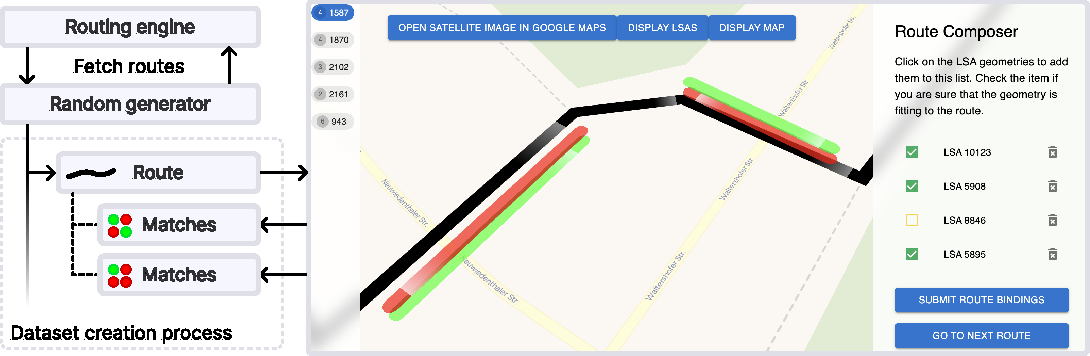
\includegraphics[width=\linewidth]{images/sg-selection-ground-truth.pdf}
\caption{The Route Composer web application.}
\label{fig:sg-selection-ground-truth}
\end{figure}

To create examples for optimal selections of traffic lights, there are multiple options. For example, one could physically ride through Hamburg along arbitrary routes and note down the most likely utilized signals. Ideally, however, the ground truth could be generated in a less time-consuming way without the need to travel to the city of Hamburg or any other remote city in which the application is deployed. 

The proposed tool "Route Composer" delivers this possibility. Instead of physically driving through Hamburg, the Route Composer is a web application that makes it possible to travel virtually along randomly generated routes and label the correct traffic lights. As shown in \Cref{fig:sg-selection-ground-truth}, the Route Composer highlights the traffic lights' and the route's geometries on a map. Then, the traffic lights can be selected by clicking on them in the web application. Once a route is finished, the selected examples are stored for model evaluation.

Independent of the way we generate examples for traffic light matching, they may be biased by limited knowledge of the intersection or personal preference, potentially leading to selections that don't represent the most likely choice. To avoid these improper selections as much as possible, two measures are employed: Assuming that the composing is done carefully enough to notice an ambiguous situation, the Route Composer provides the option to open the current intersection in Google Maps for additional cues. The second measure is a clear ruleset that determines how to handle specific situations:

\begin{enumerate}
\item Consideration is given to traffic flow and the feasibility of safely maneuvering through the intersection.
\item The intersection traversal must be entirely legal according to turn restrictions and street laws.
\item Preference is given to dedicated bicycle lanes or paths indicated by distinct markings or signage.
\item The overall continuity of the route is maintained to ensure a smooth and logical progression.
\item Lanes on the wrong roadside must be avoided.
\item Lanes should never be in an opposing direction to the route.
\end{enumerate}

Based on this ground truth, we can run a benchmark that evaluates the performance of the developed methods. For each route in the ground truth, the matching procedure is executed and produces a list of matched signals. Then, this list of traffic lights is compared to the ground truth, resulting in a number of true negatives, false negatives, true positives, and false positives. Based on these statistics, a benchmark score is calculated.

In the selection of the benchmark metric, a few more considerations are required. Since many of the thousand traffic lights can be excluded entirely by applying a rough distance threshold around the route, a large number of true negatives is expected. These easily excluded traffic lights are not of interest here. What's of interest are the traffic lights near the route for which a more thorough decision is required. Thus, a metric is required that ideally excludes true negatives. The F1 score is chosen here since it only considers true positives (TP), false positives (FP), and false negatives (FN): 

\begin{equation}
\text{F1 Score} = 2 \times \frac{\text{Precision} \times \text{Recall}}{\text{Precision} + \text{Recall}} \quad \text{where} \quad \text{Precision} = \frac{TP}{TP + FP} \quad \text{and} \quad \text{Recall} = \frac{TP}{TP + FN}
\end{equation}

Assuming that especially false-positive or false-negative matches limit the speed advisory's perceived usability, the F1 score is suitable to accurately depict the perceived quality of the matching.

\subsection{Preliminary Approaches}

During the exploration process of potential methods to solve the traffic light matching problem, several methods were tested preliminarily but discarded as they did not perform as well as expected. Before we come to the successful methods for traffic light matching, it is valuable to analyze the failures and learn why these methods did not work as expected. These learnings have been crucial to shape the final solution, as will be presented afterward.

\subsubsection{H3 Approach}

The H3 approach is based on an idea by colleagues who applied a similar method to cluster inaccurately aligned GNSS paths obtaining main directions of intersection traversal and stopping points. The core of this approach is the H3 raster, which subdivides the earth primarily into hexagonal cells\footnote{Strictly speaking, the H3 raster has 12 additional pentagons on every level to complete a seamless shape. See: \url{https://h3geo.org/docs/core-library/restable/}}. On the top resolution level (1), there are 122 cells covering the earth's surface. On level 2, the 122 cells are subdivided into 842 cells, and so forth. As a result, the H3 model contains 15 levels, which are hierarchically connected in a tree structure. Through this hierarchical structure, it is possible to efficiently navigate through the index, e.g., to find neighbor cells. 

In the work by colleagues, after the GNSS samples of each user track were assigned to an H3 cell, the resulting cells each contained a number of samples and travel direction (edge of the H3 cell), resembling a histogram of the trajectories spatially aligned with the intersections. Assuming a normally distributed GNSS scattering around the actual position, the buckets could then be used to statistically sift out the most frequently used pathways of cyclists. Minor GNSS errors or individualities in the user movement don't fall into weight as they are clustered together. Since this approach was described as remarkably successful, the fundamental idea was further explored to identify potential methods for aligning the traffic light geometries with the inaccurate bike route.

\begin{figure}[htbp]
\centering
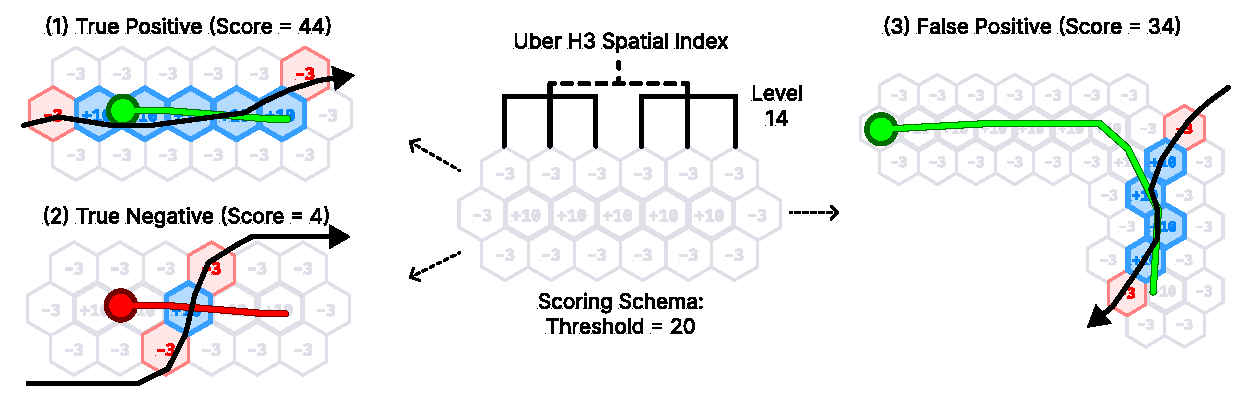
\includegraphics[width=\linewidth]{images/sg-selection-h3-approach.pdf}
\caption{Illustration of the matching procedure behind the developed H3 approach.}
\label{fig:sg-selection-h3-approach}
\end{figure}

The initial idea was to count the cells aligned between route geometry and traffic light geometries. If sufficient overlap is found, the traffic light is detected as a match. After testing multiple H3 levels, the H3 level 14 was determined empirically to provide the best tradeoff between resolution and tolerance to imperfect alignment. To emphasize the importance of a near-parallel alignment, a ring-based scoring schema as illustrated in \Cref{fig:sg-selection-h3-approach} was tested that penalizes crossing geometries (2) and favors parallel-aligned geometries (1). This ring-based scoring schema makes use of H3's tree structure to efficiently find neighboring cells of the traffic light geometry.

Nonetheless, a very significant challenge is to find a suitable scoring threshold for the number of matched cells until a traffic light is counted as a "match." Some traffic light geometries may be only a few meters long, while others are much longer. Since longer geometries contain more cells, it is more likely that longer geometries are false-positively matched to the route, while short geometries often produce false negatives. After testing multiple different scoring schemas and thresholds and coming to the final scoring schema highlighted in \Cref{fig:sg-selection-h3-approach}, it was not possible to achieve a sufficiently good matching. In the developed benchmark, an F1 score of 50\% was never exceeded. 

One identified possibility for improvement was to apply a relative scoring schema for each signal. Instead of applying absolute values to each H3 cell around the line geometry, the scoring schema would be scaled inversely proportional to the number of cells. This means that a longer line geometry would have more cells with lower individual scores compared to a short geometry. Ideally, the result would be a normalized alignment score for each traffic light geometry that can be subjected to a universal threshold. Figuratively, the score would depict how much both geometries align. However, this potential solution was not thoroughly explored due to other systematic limitations of the H3 approach.

\begin{figure}[htbp]
\centering
\includegraphics[width=\linewidth]{images/sg-selection-h3-example.png}
\caption{Example of four traffic lights that were matched using the H3 approach along the route.}
\label{fig:sg-selection-h3-example}
\end{figure}

The main limitation of the H3 approach is that it assumes that the route geometry is near enough to the matching traffic light geometries. However, considering OpenStreetMap's mixed coverage of bike paths, many false negatives were produced when the route was mapped on the car lanes, while the appropriate bike traffic light was located on the bike path a few meters to the side of the road. 

A potential solution to this problem would be to choose a larger raster, but this would worsen the score even more since many signals' geometries are no longer captured adequately. Instead, they would resemble a circular "blob", as highlighted on the left side of \Cref{fig:sg-selection-h3-example}. The "blob" problem does not only appear when upscaling the raster to H3 level 13. It appears at level 14 as well. Some traffic lights would have such short geometries that only one H3 cell was matched, especially concerning pedestrian traffic lights crossing the road. Since many of these traffic lights are aligned orthogonally to the road's direction, the loss of the signal's direction information in the "blob"-shaped scoring schema would ultimately lead to erroneous matchings. Increasing the resolution level to 15 would mitigate this problem and introduce a more shaped raster around the line geometries, but would again increase the volatility against offset traffic lights along the route.

Due to these issues, the H3-based approach for traffic light matching was not further explored. The takeaway from this approach is that close alignment does not sufficiently model matching traffic lights along a route geometry. Instead, sometimes, the traffic light geometries may be offset from the route, especially if the route is snapped onto the car lanes.

\subsubsection{Graph Approach}

The second approach is inspired by the map-matching procedure proposed by Newson and Krumm in 2009 \cite{newson_hidden_2009}. Their proposed method matches GNSS trajectories to the road network by building a transition graph between each GNSS sample and the nearby roads. After the graph is created, each transition is marked with a transition probability. In their approach, the most probable path through the transitions is calculated using the Viterbi algorithm to find the most likely sequence of roads that were taken. This approach can be transferred over to traffic light matching, interpreting the route geometry as GNSS trajectory and the traffic light geometries as road segments.

\begin{figure}[htbp]
\centering
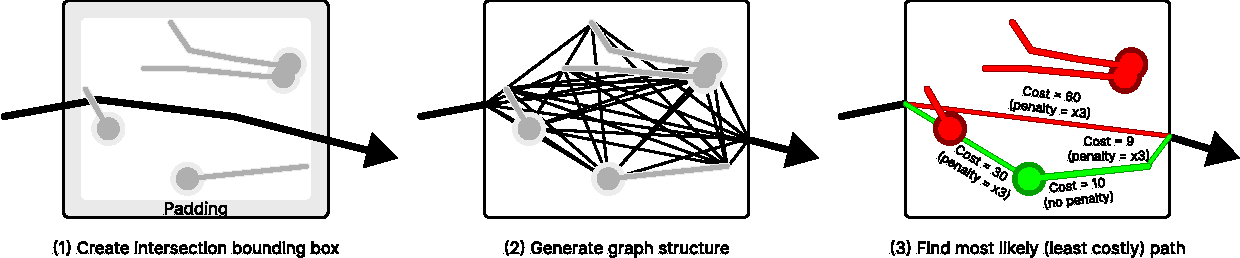
\includegraphics[width=\linewidth]{images/sg-selection-graph-approach.pdf}
\caption{Steps for traffic light matching in the graph-based approach.}
\label{fig:sg-selection-graph-approach}
\end{figure}

The proposed approach operates as illustrated in \Cref{fig:sg-selection-graph-approach}. First, traffic lights along the route are prefiltered using a rough distance threshold of 20m. The remaining traffic lights are clustered into intersections based on the intersection node ID. Around each of these intersections, the procedure undergoes three steps: (1) A bounding box is calculated with an additional padding. The route enters and exits the bounding box at one point. (2) A fully connected graph is generated between the route's entry and exit points and each traffic light geometry's start and end points. (3) A cost is assigned to each transition in the graph based on the transition's length. Finally, the least costly path is calculated using the Dijkstra pathfinding algorithm. The idea is that the least costly path represents the most likely utilized trajectory over the traffic light geometries.

The cost function is defined to penalize traversal between signals, and traversal using the traffic lights is preferred. Otherwise, the most optimal path would always be the direct connection between the entry and exit points. Specifically, every transition in the graph  $(p_{1} \rightarrow p_{2})$ has the cost $dist(p_{1}, p_{2})$, while transitions between traffic lights have the cost $dist(p_{1}, p_{2}) \times \text{penalty}$. Thus, the penalty value represents a hyperparameter of the model together with the dimensions of the intersection padding. 

Which penalty value and intersection padding to choose may depend on each intersection's characteristics. Thus, defining these hyperparameters by hand would not be the best option. A better option is to utilize a tuning algorithm that automatically approximates the optimal configuration based on the developed ground truth. Specifically, the Tree-Structured Parzen Estimator hyperparameter tuning algorithm \cite{ozaki_multiobjective_2020} is utilized. This tuner considers each hyperparameter (intersection padding and penalty) independently from each other. During the tuning, the model undergoes inference for all routes in the dataset (one trial). After each of these trials, the F1 score is evaluated, and the hyperparameters are adjusted by the tuner into a direction the tuner estimates will result in a better score.

\begin{figure}[htbp]
\centering
\includegraphics[width=\linewidth]{images/matching-dijkstra-correct.pdf}
\caption{Examples of correct matching using the graph approach.}
\label{fig:sg-selection-graph-example}
\end{figure}

After tuning the model to the ground truth, the model reached an F1 score of 75.4\% (penalty = 2.87, padding = 25m). As a distance function, this version of the model utilizes the Euclidean distance between the coordinates in the WGS84 projection system. Correct matchings from this model highlighted in \Cref{fig:sg-selection-graph-example} indicate the model's capabilities. The model would perform well even in scenarios where the signal's geometry is offset to the route and thus has large advantages over the H3 approach, as reflected in the improved F1 score.

\begin{figure}[htbp]
\centering
\includegraphics[width=\linewidth]{images/matching-dijkstra-incorrect.pdf}
\caption{Examples of false matching using the graph approach.}
\label{fig:sg-selection-graph-fails}
\end{figure}

However, the final result is still not convincing, considering that the measured score of 75.4\% represents a training F1 score and was not evaluated on unseen data. By studying many error cases, one particular weakness was identified. As highlighted in \Cref{fig:sg-selection-graph-fails}, the model would struggle particularly with right or left turns at intersections. In these cases, the route exits the bounding box on an adjacent edge to the ingress's edge. This means that the direct distance from the ingress point to the egress point is often lower than the path over the correct signals' geometries. As a result, the model tends to shortcut directly to the intersection exit. To cope with these cases, two potential solutions were identified:

\begin{enumerate}
    \item Increasing the penalty for traveling off a signal's geometry. A separate penalty could be applied in cases where the ingress and egress edges of the bounding box are adjacent to avoid shortcuts.
    \item  Modifying the graph generation procedure to strictly "go back" to the nearest point on the route after each traversal of a signal's geometry. Thus, the penalty for attempted shortcuts (going off the route) would increase drastically.
\end{enumerate}

Option one initially may seem like a good choice here. However, this strategy would worsen another problem highlighted in \Cref{fig:sg-selection-graph-fails}: often, traffic light geometries are falsely traversed simply because their exit point is slightly more proximal to the egress point. A higher penalty amplifies this problem. Thus, option two was implemented instead. 

\begin{figure}[htbp]
\centering
\includegraphics[width=\linewidth]{images/matching-dijkstra-strict.pdf}
\caption{Examples of matching using the adjusted graph generation procedure.}
\label{fig:sg-selection-graph-strict}
\end{figure}

Unfortunately, the result of the adjusted graph generation procedure is a worse F1 score after hyperparameter tuning of 60.7\% (penalty = 9.68, intersection padding = 42m). In many cases, the model would now avoid shortcutting as intended, but the model would also be noticeably more strict. The reason is that the signals' geometries are no longer connected to each other but rather through the route (see \Cref{fig:sg-selection-graph-strict}). Jumping on and off the signals' geometries would often be a worse option for the pathfinding algorithm than staying on the route, even with a remarkably higher penalty. 

Another variation of the graph-based approach would be to cut out the intersections, reconnect the OpenStreetMap paths via the traffic light geometries, and then calculate the route using these. However, the main problems here would probably be similar, especially the problem of connecting the traffic light geometries with each other and the problem of stitching at the edges. Thus, this idea was not further explored.

Although the developed graph-based methods initially promised good results, they were ultimately not further studied in favor of more promising ideas. Even if the graph approach seems less susceptible to offsets and longer traffic light geometries, it clearly falls short when considering the curvature and not only the absolute location of the traffic light geometries. In the end, only each traffic light geometry's start and end points are considered. However, the curvature is similarly important to decide which traffic light could match the associated route.

\subsubsection{Map-Matching Approach}

A positive learning of the graph-based approach is that the map-matching problem of Newson and Krumm (2009) \cite{newson_hidden_2009} is, in theory, very similar to the problem we are trying to solve. Another idea based on this approach would be to map-match the traffic light geometries onto the OpenStreetMap road network, fusing both map sources and allowing for a direct traffic light lookup.

\begin{figure}[htbp]
\centering
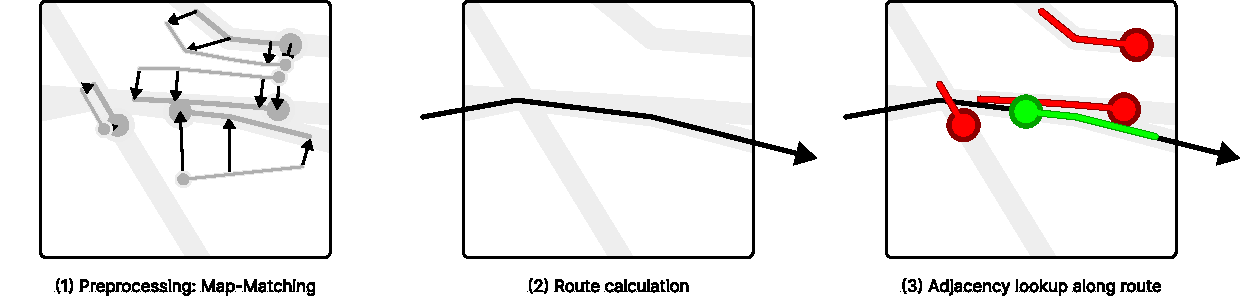
\includegraphics[width=\linewidth]{images/sg-selection-map-matching-approach.pdf}
\caption{Steps for map-matching traffic lights onto the routing foundation.}
\label{fig:sg-selection-map-matching-approach}
\end{figure}

\Cref{fig:sg-selection-map-matching-approach} illustrates the proposed procedure, consisting of three steps: (1) In a preprocessing step, the traffic light geometries are map-matched onto the routing foundation. As a result, the traffic light geometries align with the routing foundation's topology. (2) The route is calculated using the same routing foundation. (3) All traffic lights that perfectly align with the route's geometry are matched.

The approach by Newson and Krumm (2009) \cite{newson_hidden_2009} is utilized as a map-matching procedure. This approach is implemented by default in the GraphHopper routing engine and can be accessed through its map-matching API\footnote{\url{https://docs.graphhopper.com/\#tag/Map-Matching-API}}. Each traffic light geometry is transformed into a compatible format (GPX) and sent to the map-matching API, where it is projected onto the integrated routing foundation.

\begin{figure}[htbp]
\centering
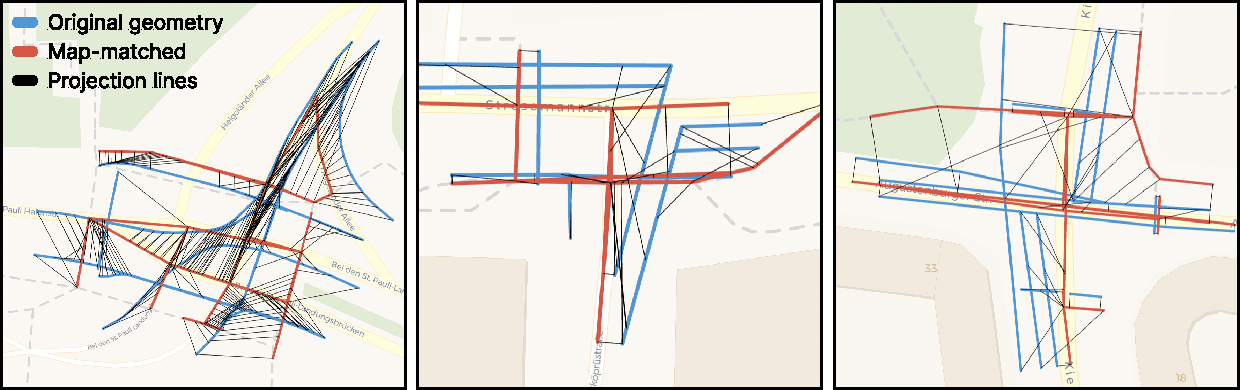
\includegraphics[width=\linewidth]{images/sg-selection-map-matching-fails.png}
\caption{Distortion of traffic light geometries after map-matching.}
\label{fig:sg-selection-map-matching-fails}
\end{figure}

Despite the promising idea, when testing the approach with the OpenStreetMap routing foundation, a substantial problem was determined. Although it was possible to project the traffic light geometries onto the routing foundation, they were completely distorted during the process. Examples of this distortion are highlighted in \Cref{fig:sg-selection-map-matching-fails}. These distortions may be amplified by the problem that traffic light geometries are usually shorter than typical GNSS trajectories for which the map-matching approach was initially conceived. What's clear is that, without enough intersection detail in the routing foundation, the map-matching procedure would often fail to find a suitable projection. Moreover, multiple traffic lights may be matched onto the same path segment, resulting in an ambiguous matching. 

Since not only bike traffic lights are represented in the system but also traffic lights shared between cars/buses and bikes, this approach would require a routing foundation that represents all of the respective paths (not only bike paths) noticeably more accurately than OpenStreetMap, such as a multimodal HD map. Whether this approach applies to such a map could not be tested as none was available. Due to these findings, the map-matching method was also not investigated further.

\subsection{Algorithmic Filtering Approach}

The preliminary H3, graph, and map-matching approaches have not been successful but provided a deeper understanding of the problem. First, an ideal matching procedure should be robust against offsets of the traffic light geometries from the route, especially in cases when the route geometry is mapped on the road while the bike traffic light is alongside. Second, the matching procedure must handle long and short traffic light geometries similarly well. 

\begin{figure}[htbp]
\centering
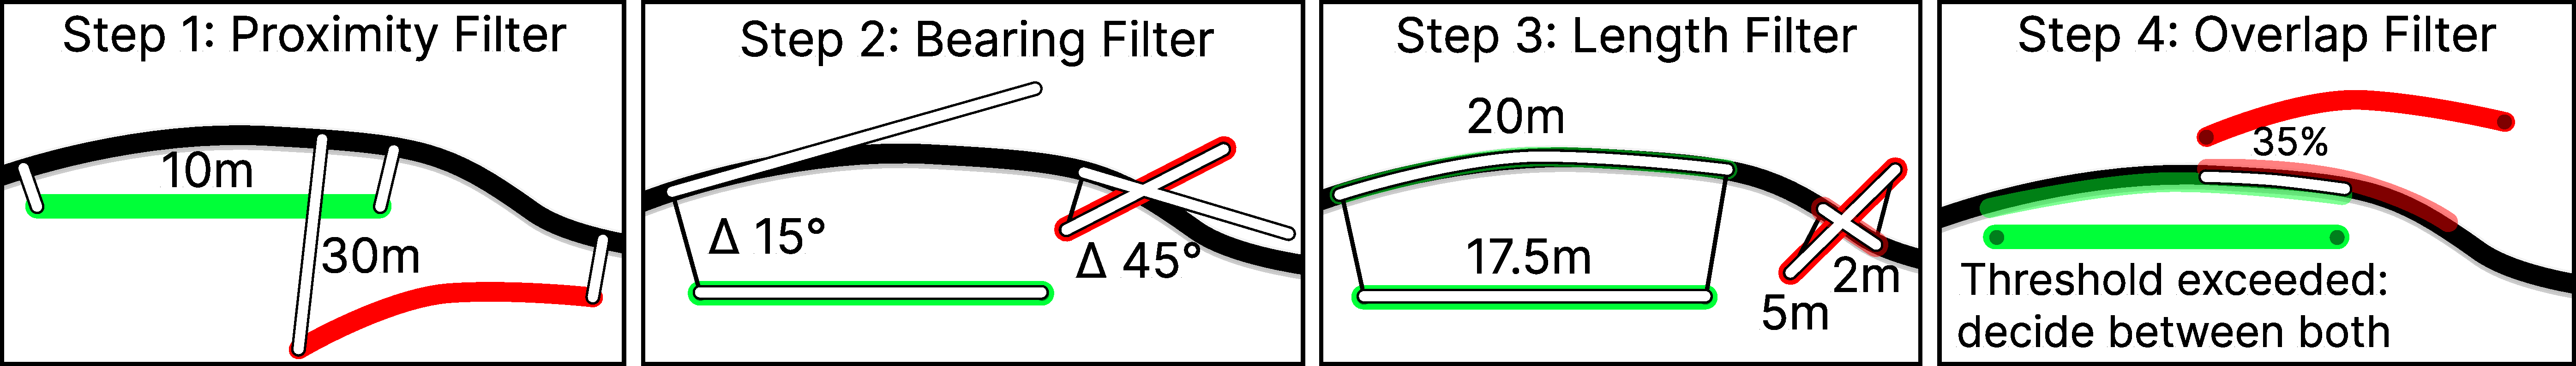
\includegraphics[width=\linewidth]{images/sg-matching-filters.pdf}
\caption{Filtering steps for matching with the algorithmic approach.}
\label{fig:sg-matching-filters}
\end{figure}

Most importantly, it is crucial to consider the absolute location of the traffic light geometries along the route and their geometrical properties in relation to the route. If the signal's geometry is aligned relatively near the route and follows its curvature, it is likely to match the route. The question is how to mathematically model this relation and tell apart edge cases.

One solution is to tell apart matching from non-matching traffic light geometries by a geometrical comparison with the route. In four filtering steps, specific geometric thresholds are applied to filter out traffic lights that are likely no match. The idea is that each step catches a specific type of misalignment with the route, such that, in the end, only the wanted matches remain. As shown in \Cref{fig:sg-matching-filters}, four filtering steps are employed: proximity filter, bearing filter, length filter, and overlap filter.

\paragraph{Step 1 -- Distance Filter:} Step one focuses on coarsely excluding a large proportion of the traffic lights in the city area through a distance threshold $t_{dist}$ from the route. This step is efficiently executed through a PostGIS database using the \texttt{ST\_Distance}\footnote{\url{https://postgis.net/docs/en/ST\_Distance.html}} query.

\paragraph{Step 2 -- Bearing Filter:} As a next step, the bearing between the signal's geometry and the route is compared. Hereby, we can exclude traffic lights that are angled too steeply or even inverted to the route. As a foundation, the atan2 function is used to calculate the bearing between two coordinates on the earth\footnote{\url{https://www.movable-type.co.uk/scripts/latlong.html}}:

\begin{equation}
x(c_1, c_2) = sin(lon_2 - lon_1) \times cos(lat_2)
\end{equation}
\begin{equation}
y(c_1, c_2) = cos(lat_1) \times sin(lat_2) - (sin(lat_1) \times cos(lat_2) \times cos(lon_2 - lon_1))
\end{equation}
\begin{equation}
bear(c_1, c_2) = atan2(x(c_1, c_2), y(c_1, c_2))
\end{equation}

where $c_1 = (lat_1, lng_1)$ and $c_2 = (lat_2, lng_2)$ are WGS84 coordinates (in radians). As a result, we can calculate the bearing of the signal's geometry $(c_1, \dots, c_n)$ based on its first two coordinates. To compare this bearing to the route geometry, the signal's geometry is projected onto the route. Every coordinate $(c_1, \dots, c_n)$ is mapped to the nearest point on the route geometry $(\bar{c_1}, \dots, \bar{c_n})$. Then, the bearing diff $\bar{\Delta}_{bear_1}$ is calculated as:

\begin{equation}
    \bar{\Delta}_{bear_{i=1}} = 
        abs(\underbrace{bear(c_{i=1}, c_{i+1=2})}_{\text{Bearing of traffic light geometry}} - \underbrace{bear(\bar{c}_{i=1}, \bar{c}_{i+1=2})}_{\text{Bearing of projection on route}})
\end{equation}

The bearing diff $\bar{\Delta}_{bear_1}$ denotes how much the signal's angle is different from the route's angle at the nearest point to the first traffic light geometry coordinate. The calculated value can be subjected to a bearing threshold $t_{bear}$ which defines if the signal's geometry is counted as a match or not:

\begin{equation}
\Psi_{bear_{i=1}} = 
    \begin{cases}
            1,& \text{if } \bar{\Delta}_{bear_{i=1}} \in \left(-t_{bear}, t_{bear}\right)\\
            0,              & \text{otherwise}
        \end{cases}
\end{equation}

where $\Psi_{bear_{i=1}} = 1$ means that the segment is angled similarly enough to the nearby route and is therefore a match. All traffic lights that are not a match ($\Psi_{bear_{i=1}} = 0$) are filtered out. For example, if $t_{bear} = 45°$, we will filter out all geometries whose first coordinate is angled more than $\pm 45°$ relative to the projection onto the route. 

\begin{figure}[htbp]
\centering
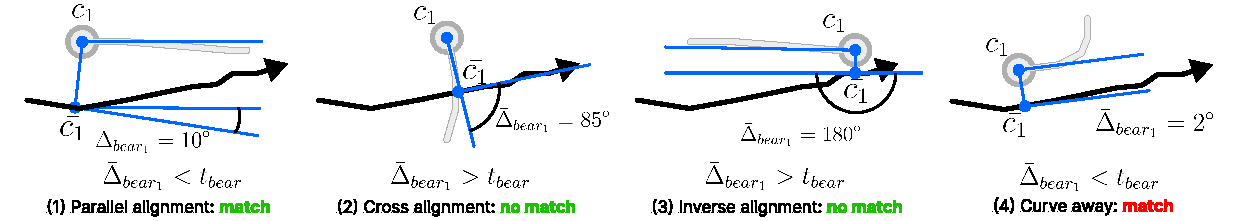
\includegraphics[width=\linewidth]{images/sg-selection-bearing-filter.pdf}
\caption{Examples for bearing matching based on traffic light geometry's first coordinate.}
\label{fig:sg-selection-bearing-filter}
\end{figure}

This process is drawn in \Cref{fig:sg-selection-bearing-filter}. In cases (1), (2), and (3), the alignment of both geometries is classified correctly. However, (4) illustrates one particular weakness: traffic light geometries initially aligned but then curving away from the route are not filtered out correctly. The reason is that only the first coordinate is compared, and not the complete geometry. To compare the complete geometry, all coordinates $c_i$ of the traffic light geometry are compared to the route. Then, a weighted sum $\phi_{bear}$ is calculated, incorporating the length of each geometry segment relative to the complete geometry. In this way, longer parts of the signal's geometry are emphasized:


\begin{equation} 
\phi_{bear} = 
    \underbrace{\sum_{i=1}^{n-1} 
    \frac{\Psi_{bear_i}}{dist(c_i, c_{i+1})}}_{\text{Sum of matching segment lengths}}
    \times
    \underbrace{(\sum_{i=1}^{n-1} dist(c_i, c_{i+1}))^{-1}}_{\text{Sum of segment lengths}}
\end{equation}

where $dist$ is calculated as the Euclidean distance and $n$ is the number of coordinates in the signal's geometry. As a result, $\phi_{bear}$ is normalized between 0 and 1. $\phi_{bear} = 0$ means none of the traffic light geometry's segments matches the angular threshold $t_{bear}$, while a value of 1 represents a full match. To determine the decision boundary between match and no match, $\phi_{bear}$ is subjected to another threshold $t_{bear\_sum} \in [0, 1]$. This threshold is chosen such that traffic lights curving away from the route are also excluded.

\begin{figure}[htbp]
\centering
\includegraphics[width=\linewidth]{images/sg-selection-bearing-filter-sum.pdf}
\caption{Examples for (cumulative) bearing matching.}
\label{fig:sg-selection-bearing-filter-sum}
\end{figure}

\Cref{fig:sg-selection-bearing-filter-sum} gives an intuition for the final working principle of the bearing filter. In example (1) all segments of the signal's geometry are sufficiently aligned to the route. Examples (2) and (3) depict cases where none of the segments are within the angular threshold $t_{bear}$. Example (4) highlights a case where the first 60\% of the traffic light geometry matches the route. In the illustration, $t_{bear\_sum}$ is assumed to be larger than 60\%, and so the traffic light that curves away is filtered out. The higher this threshold is configured, the more aggressively the filter excludes inclined geometries.

\paragraph{Step 3 -- Length Filter:} With the previous two steps, we have two bearing thresholds ($t_{bear}$ and $t_{bear\_sum}$) in addition to the distance threshold $t_{dist}$. However, during the systematic testing of the thresholds it quickly became clear that these thresholds alone are not nearly enough to sufficiently distinguish matching from non-matching signals. During the search for other characteristics that distinguish matching from non-matching signals, a key observation was made: Non-matching traffic light geometries often have a shorter projection onto the route relative to their original length. This feature is also related to the traffic light geometry's angular position to the route but incorporates the shape of the route in between projected traffic light geometry coordinates.

\begin{figure}[htbp]
\centering
\includegraphics[width=\linewidth]{images/sg-selection-length-filter-sum.pdf}
\caption{Examples for (cumulative) length matching.}
\label{fig:sg-selection-length-filter-sum}
\end{figure}

To mathematically represent this intuition, a cumulative score $\phi_{len}$ is calculated similarly to the bearing filter and then subjected to a threshold $t_{len\_sum}$. The score $\phi_{len}$ quantifies the difference from 0 (no matching segments) to 1 (all segments matching), again weighted by the length of each segment. Example (3) shows that the length filter is not good at detecting inversely aligned geometries. However, since the bearing filter is assumed to handle this case, the length filter will likely not encounter such constellations.

Due to the similarity with the bearing filter, we can reuse its formulas and only have to replace the metric $\Psi$, which determines whether a segment is counted as a match. First, each segment $(c_1, \dots, c_n)$ is again projected onto the route as $(\bar{c_1}, \dots, \bar{c_n})$. Then, the length diff $\bar{\Delta}_{len_1}$ for the i-th segment is calculated as:

\begin{equation}
    \bar{\Delta}_{len_i} = 
        \begin{cases}
            0,& \text{if } line\_dist(\bar{c}_i, \bar{c}_{i+1}) = 0 \\
            abs(\frac{dist(c_{i}, c_{i+1})}{line\_dist(\bar{c}_{i}, \bar{c}_{i+1})}),              & \text{otherwise}
        \end{cases}
\end{equation}

where $dist$ is calculated as the Euclidean distance, and $line\_dist(\bar{c}_i, \bar{c}_{i+1})$ represents the distance along the route's geometry between $\bar{c}_i$ and $\bar{c}_{i+1}$. To calculate $line\_dist$, it is necessary to interpolate along the route's geometry. Using the calculated length diff, each segment of the signal's geometry is mapped as:

\begin{equation}
\Psi_{len_i} = 
    \begin{cases}
            1,& \text{if } \bar{\Delta}_{len_{i}} \in \left(1 - t_{len}, 1 + t_{len}\right)\\
            0,              & \text{otherwise}
        \end{cases}
\end{equation}

where $\Psi_{len_i} = 1$ means the segment matches the length diff threshold $t_{len}$. Finally, the weighted sum of all traffic light geometry segments is calculated as follows:

\begin{equation} 
\phi_{len} = 
    \underbrace{\sum_{i=1}^{n-1} 
    \frac{\Psi_{len_i}}{dist(c_i, c_{i+1})}}_{\text{Sum of matching segment lengths}}
    \times
    \underbrace{(\sum_{i=1}^{n-1} dist(c_i, c_{i+1}))^{-1}}_{\text{Sum of segment lengths}}
\end{equation}

Here, $\phi_{len} = 0$ means that all of the traffic light geometry's segments are shortened too much when projecting them onto the route geometry, indicating a traffic light that is not aligned with the route. Likewise, $\phi_{len} = 1$ means that all segments roughly stay the same length when projected onto the route. To distinguish when a traffic light is counted as a match or not, the thresholds $t_{len}$ and $t_{len\_sum}$ can be optimized accordingly.

\paragraph{Step 4 -- Overlap Matcher:} The previous matching steps often struggle with one particular problem: multiple parallel-aligned signals. Often, this case leads to a multi-selection of these signals, while only one of them will be taken by the cyclist. On the other hand, especially on complex intersections, there may be multiple consecutive traffic lights whose geometries partially overlap along the route but are still a valid match. Thus, some overlaps need to be filtered out, while others are intentional.

\begin{figure}[htbp]
\centering
\includegraphics[width=0.5\linewidth]{images/overlap.drawio.pdf}
\caption{Example overlap.}
\label{fig:sg-matching-overlap-filter}
\end{figure}

First, the overlaps between traffic lights with respect to the route are determined. To accomplish this, the signals' geometries are snapped onto the route. As a result, each signal's start and end points along the route are determined, as highlighted in \Cref{fig:sg-matching-overlap-filter}. For each pair of matched traffic light geometries $(l_1, l_2)$, an overlap percentage $\phi_{overlap}$ is calculated as:

\begin{equation}
    \phi_{overlap} = \frac{min(l_{1_{end}}, l_{2_{end}}) - max(l_{1_{start}}, l_{2_{start}})}{max(l_{1_{end}}, l_{2_{end}}) - min(l_{1_{start}}, l_{2_{start}})}
\end{equation}

In the error case that the denominator is zero, $\phi_{overlap}$ is also mapped to zero. As soon as this percentage exceeds a threshold $t_{overlap\_pct}$, a decision process between both geometries is initiated:

\begin{enumerate}
    \item According to the traffic light metadata, if one of the traffic lights is a dedicated bike signal, choose that one.
    \item If one of both traffic lights perfectly matches the route, select that one. To determine whether a traffic light perfectly matches the route, a distance threshold $t_{perfect\_match}$ is configured.
    \item If both traffic lights are on different sides of the route and the distance between both traffic lights is smaller than a threshold $t_{road\_side}$, prefer the ordinary traffic side (in Germany, right-hand traffic). Whether a traffic light is left or right from the route is determined through $\bar{\Delta}_{bear_{i=1}}$.
    \item Otherwise, decide purely by the distance to the route.
\end{enumerate}

The thresholds $t_{overlap\_pct}$, $t_{perfect\_match}$, and $t_{road\_side}$ can be used to tune the final result. In the case of $\phi_{overlap} < t_{overlap\_pct}$, both traffic lights are kept. This allows for intentional small overlaps at complex intersections without filtering one of both traffic lights out.

\begin{table}[h]
\caption{Summary of thresholds and search space.}
\begin{tabular}{@{}lp{9.5cm}l@{}}
\toprule
\textbf{Hyperparameter}  & \textbf{Explanation} & \textbf{Search Interval} \\
T1 ($t_{dist}$) & Traffic light geometries must be within this distance of the route. & $[1m, 100m]$ \\
T2 ($t_{bear\_sum}$) & The minimum proportion of the signal's geometry matching $t_{bear}$. & $[0, 100\%]$ \\
T3 ($t_{bear}$) & If segments of the traffic light geometry are angled more steeply to the route than this value, they are not counted for $t_{bear\_sum}$. & $[0°, 180°]$ \\
T4 ($t_{inv}$) & Whether inverted traffic light geometries should be matched. & $[\text{False}, \text{True}]$ \\
T5 ($t_{len\_sum}$) & The minimum proportion of the signal's geometry matching $t_{len}$. & $[0, 100\%]$ \\
T6 ($t_{len}$) & If segments of the traffic light geometry are elongated or shortened more than $1 \pm t_{len}$ when projected onto the route, they are not counted for $t_{len\_sum}$. & $[0, 1]$\\
T7 ($t_{road\_side}$) & If two overlapping traffic lights are on opposite sides of the route and less than this distance away from each other, decide by the ordinary traffic side. & $[0, 100m]$ \\
T8 ($t_{perfect\_match}$) & If a signal's geometry is closer to the route than this value, it is preferred over another overlapping traffic light geometry. & $[0, 50m]$ \\
T9 ($t_{overlap\_pct}$) & If two traffic lights overlap more relative to their combined length, a decision process between both traffic lights is initiated. & $[0, 100\%]$ \\
\bottomrule
\end{tabular}
\label{tab:hyperparameter-space}
\end{table}

\paragraph{Model Finetuning:} The designed filtering pipeline has several thresholds that must be carefully selected to optimize the final matching performance. Here, it is important to consider that each filter influences the subsequent filters in the pipeline. This means that it is difficult and time-intensive to tune the individual filters by hand. A solution to this problem is utilizing a hyperparameter tuning algorithm, which tries to understand the influence of each hyperparameter on a model and maximizes its score. This algorithm can run overnight, resulting in a proposed model configuration after a few hundred to thousand trials. To prepare the model for hyperparameter tuning, search spaces for each hyperparameter must be defined. These search spaces are summarized in \Cref{tab:hyperparameter-space}. The Tree-Structured Parzen Estimator hyperparameter tuning algorithm \cite{ozaki_multiobjective_2020} is utilized to find a good configuration on the ground truth benchmark. The objective function given to the tuner algorithm is the F1 score.

\subsection{Machine Learning Filtering Approach}

One identified problem of the algorithmic approach is that each threshold is defined globally and equally applied to all situations. However, not all intersections are crossed similarly by routes. Thus, the filtering pipeline would be applied too strictly in some situations, while the thresholds are not applied strictly enough in others. Here, a machine learning model can be useful to employ a more flexible and interlinked mapping of the geometric properties.

Regarding the problem of deciding between "match" and "no match" for each traffic light geometry, there may be many creative ways to establish a machine learning classifier. For example, it would be possible to generate top-down images of each intersection and utilize machine-learning techniques from image detection or segmentation to classify each signal. However, as a rule of thumb, more complicated tasks tend to require larger machine learning models, which in turn require a larger ground truth. 

Unfortunately, the ground truth itself would ever be able to contain a few thousand unique samples at most, which speaks against the viability of applying more advanced deep learning models. Dataset augmentation through artificial distortion of the traffic light geometries was found in preliminary experiments not to be a purposeful option. A meaningful balance between marginally distorting the traffic light geometries and invalidating the labeling could not be identified. Furthermore, there would be the concern of scalability with larger models and a more complex feature processing pipeline. Thus, the decision was made to opt for a more conservative approach.

\begin{figure}[htbp]
\centering
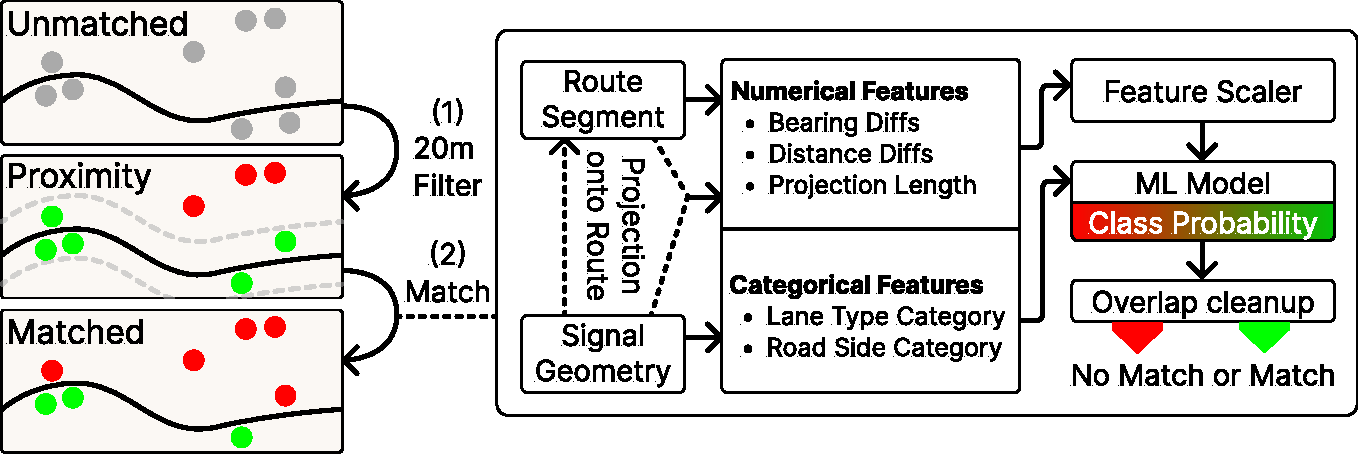
\includegraphics[width=\linewidth]{images/sg-matching-ml-model.pdf}
\caption{Filtering steps for matching with the machine learning model.}
\label{fig:sg-matching-ml-model}
\end{figure}

The proposed approach (see \Cref{fig:sg-matching-ml-model}) operates as follows: The bearing, length, and overlap filtering steps from the algorithmic approach are removed and replaced with a single "Match" step to incorporate the machine learning classifier into the filtering process. During this step, the signal's geometry is first projected onto the route. The result of this step is one sample incorporating the traffic light geometry and the projected traffic light geometry onto the route. It is important to note here that each sample considers one signal, not a complete intersection. Based on the sample, numerical and categorical features are calculated that represent the geometrical relationship between the route and the traffic light geometry.

The numerical features are subjected to a feature scaler to prepare them for model inference. The categorical features are calculated or extracted from the traffic light metadata. Both numerical features and categorical features are input into the machine learning model. As a result, the machine learning model produces a class probability for "match" or "no match." The class probability is utilized in an additional overlap cleanup step (similar to the algorithmic approach's overlap filter) to obtain the final matching traffic lights along the route.

\paragraph{Feature and Model Grid Search:} To select a suitable machine learning model architecture and feature processing pipeline, gathered experiences from hyperparameter tuning were utilized to systematically and rigorously identify promising configurations. Out of the tested traditional model architectures including k-Nearest-Neighbors (k-NN), Decision Tree, Random Forest, Multilayer Perceptron (MLP), AdaBoost, Gaussian Naive Bayes, Quadratic Discriminant Analysis (QDA), and Support Vector Machine (SVM), the MLP model overall performed the best and was thus selected as the final classifier, after testing other promising models with different feature constellations. 

To ensure comparability during the model testing process, each model feature pipeline was trained and tested using the stratified variant of the k-fold cross-validation\footnote{\url{https://scikit-learn.org/1.3/modules/generated/sklearn.model_selection.StratifiedKFold.html}}. As there are many more non-matching traffic lights along routes in the ground truth than matching signals, this variant ensures that a similar balance is present in each generated training/testing split of the ground truth dataset. By looking at the models' scores and the mutual information of each feature, some features were discarded as they provided no additional information. The final feature set is as follows:

\begin{itemize}
    \item The lane type of the signal. This property is extracted from the signal's metadata and one-hot-encoded.
    \item The road side of the signal. To calculate this property, it is determined on which side of the route the first coordinate of the traffic light geometry is located.
    \item The maximum and minimum bearing diffs between the traffic light geometry segments and their projections onto the route ($\bar{\Delta}_{bear_i}$).
    \item The change in route bearing from the first to the last route segment. 
    \item The first, last, and shortest distance between traffic light geometry coordinates and their projections onto the route.
    \item The length of the traffic light geometry's projection onto the route.
\end{itemize}

A feature scaling algorithm is employed to optimize the machine learning model's learning and inference process. Here, it is usually a good option to choose a Yeo-Johnson power transformation \cite{yeo_new_2000}, which includes standardization and additionally tries to symmetrize the observed data into a normal distribution. Together with the scaled numerical features, the one-hot-encoded categorical features are input into the model as, in sum, 16 features. Together with the model, the parameters of the Yeo-Johnson power transformation are only fit to the dataset's training proportion.

\begin{figure}[htbp]
\centering
\includegraphics[width=\linewidth]{images/sg-selection-overlap-cleanup.png}
\caption{Model selection without (left) and with (right) overlap cleanup.}
\label{fig:sg-selection-overlap-cleanup}
\end{figure}

\paragraph{Overlap Cleanup:} As in the algorithmic approach, there may be some cases where multiple overlapping traffic lights are selected. These duplicate selections may happen when multiple traffic light geometries are very closely aligned to the route, and must be cleaned up, as the app should only focus on the most likely used signal. 

As shown in \Cref{fig:sg-selection-overlap-cleanup}, the utilized traffic light is most likely the longest of the three selected geometries. This traffic light arguably has the best alignment with the route geometry. How much the model thinks a traffic light matches the route can be measured by the output probability (neuron activation) for the two classes "match" and "no match." This feature is used to force the model to decide between overlapping signals. In case a sufficient overlap between two traffic light geometries is detected, the traffic light with the higher probability for "match" is selected. As highlighted in \Cref{fig:sg-selection-overlap-cleanup}, this process is effective at filtering out the problem.

\subsection{Integration of Unconnected Intersections}

Not all intersections have traffic lights connected to Hamburg's data broker. However, this represents a problem for matching traffic lights along a route. If an unconnected intersection lies between the user and the next connected intersection, the user may get a speed advisory for the wrong intersection. Although the traffic light is later visualized on the in-app map, this may still lead to confusion for the user. Thus, it is crucial also to identify the unconnected intersections along the bike path. These unconnected intersections are later visualized with a unique traffic light symbol in the user interface.

To find out which intersections are not connected to the system (but still signalized), the Lichtsignalanlagen Hamburg\footnote{\url{https://metaver.de/trefferanzeige?docuuid=C498DEED-985C-11D5-889E-000102B6A10E}} dataset is utilized. This dataset is updated periodically every four months and contains single coordinates of each signalized intersection in Hamburg. Thus, the dataset does not resolve individual traffic light geometries but the center locations of the intersection node. 

To identify which intersections are connected, it is determined which intersections have traffic light geometries within an empirically defined threshold of 50 meters. These intersection nodes from the Lichtsignalanlagen Hamburg dataset are marked as "connected." All other nodes are marked as "unconnected." In case of a traffic light unassigned to any intersection node, it is assumed that this intersection node is missing in the Lichtsignalanlagen Hamburg dataset, and a new intersection node is created. 

Finally, a list of intersection nodes is matched to the route by a distance threshold of 50 meters. To avoid displaying a speed advisory for a wrong intersection, the app handles each unconnected intersection like a traffic light that doesn't send any data. Once an unconnected intersection is passed before another (connected) signal, the speed advisory is enabled again. This step completes the traffic light matching pipeline.

\begin{Summary}[Summary of Methods]
Route-based traffic light matching is proposed as a novel solution to the problem of identifying traffic lights for GLOSA. The proposed method is designed to be practical for all smartphone mounting spots and invulnerable to inaccurate GNSS. Furthermore, all upcoming traffic lights are known at any time during the ride. However, a significant challenge is to precisely estimate which sequence of traffic lights will most likely be utilized by a cyclist. The approach must employ human-like spatial reasoning to tell apart non-matching from matching signals.

To develop and test mathematical models with the goal of resembling human spatial reasoning, human matchings of traffic lights along randomized routes are collected through a web tool. The resulting ground truth dataset is utilized to calculate an overall matching quality through the F1 score.

Multiple methods were tested preliminarily but not investigated further. Nonetheless, the learnings from these methods were ultimately incorporated into an algorithmic filtering pipeline. This pipeline employs geometrical filters that calculate each signal's distance, bearing, and projection length to determine whether it would suit the route. Finally, overlapping traffic lights are compared to each other to decide which one matches the route better. As a result, a sequence of traffic lights is returned, which are predicted to match a given input route.

To further improve the developed filtering pipeline, it was determined that the geometric features, such as bearing or projection length, could be weighted more dynamically by a machine learning model. The final MLP model utilizes 16 features calculated from the signal's geometry and its projection onto the route to determine if this traffic light matches the route. In case of overlaps, the traffic light predicted to match the route most likely is chosen.

Finally, to avoid speed advisories being given for a traffic light that comes after an unconnected but signalized intersection, the Lichtsignalanlagen Hamburg dataset is utilized. 
\end{Summary}

\section{Results}

- Die Evaluation des traffic light matching ist in mehrere Teile geteilt. Wir fangen bei der Datenanalyse der Ampelgeometrien an, und tasten uns dann zur Untersuchung der Ground Truth vor.
- Wir schauen ob diese repräsentativ genug ist, um qualifizierte Aussagen über die Genauigkeit der entwickelten Verfahren zu machen
- Mithilfe dieser Betrachtungen evaluieren wir anschließend die Benchmark-Performance beider Ansätze
- Außerdem schauen wir uns an, wie effektiv beide Methoden die richtigen Ampeln auswählen, selbst wenn Routingfehler vorhanden sind
- Die Skalierbarkeit und Praktikabilität des Modells untersuchen wir mithilfe einer kurzen Performance-Analyse auf einem TU-Dresden Deployment
- Zum Schluss validieren wir unsere Benchmark-Ergebnisse noch durch einen Test in Hamburg

\subsection{Study of Traffic Light Geometries in Hamburg}

- Um in die Evaluation zu starten, betrachten wir als erstes die Ampelgeometrien etwas genauer
- Im Konzept wurde beschrieben, dass die Metainformation über die von einer Ampel bedienten Verkehrsmittel ein wichtiges Entscheidungskriterium darstellen. Das entwickelte Verfahren soll sich immer dann für eine dedizierte Radfahrampel entscheiden, wenn dies durch die Kreuzungstopologie möglich ist
- Stand 8. Dezember 2023 haben 677 von 791 (85.6\%) im System verfügbaren Kreuzungsknoten mindestens eine dedizierte Fahrradampel. An 194 (24.5\%) Kreuzungen gibt es mindestens eine Ampel, die sich Radfahrer und KFZ teilen können. 53 Kreuzungen (6.7\%) besitzen mindestens eine Ampel die Mischverkehr von Radfahrern, KFZ und Bussen zugeordet ist. An 24 Kreuzungen (3\%) gibt es Ampeln geteilt zwischen Fußgängern und Radfahrern

\begin{figure}[htbp]
\centering
\includegraphics[width=\linewidth]{images/lanes-map.pdf}
\caption{.}
\label{fig:lanes-map}
\end{figure}

- Die Prozentzahlen überschneiden sich, da es häufig pro Kreuzung und Fahrtrichtung mehrere parallele Ampeln gibt, die theoretisch genutzt werden können, von denen aber nur eine schließlich die beste Wahl ist
- Schon wenn wir einzelne Einfahrtsspuren und die möglichen Abbiegungen aus dieser Einfahrtsspur betrachten, wird deutlich, dass Radfahrer häufig viele Optionen haben, in die gleiche Richtung abzubiegen. Von insgesamt 4349 Einfahrtsspuren, die für Radfahrer markiert sind, sind 653 (15\%) der Einfahrtsspuren mit mehreren Ampelgeometrien verknüpft. An der Kreuzung 177 (53°34'10.6"N 10°03'22.1"E) haben Radfahrer beispielsweise die Möglichkeit, aus einer einzigen Einfahrtsspur in 4 Spuren rechts, 4 Spuren links, und 1 Spur geradeaus abzubiegen. 
- Auch wenn in der Regel mehrere Connections simultan schalten und in diesem Fall eine Falschauswahl nicht zwangsweise zu einer falschen Geschwindigkeitsempfehlung führt, muss damit gerechnet werden, dass die unterschiedlichen Abbiegerichtungen auch durch separat schaltende Signalgeber bedient werden.
- In diesem Fall ist die Auswahl rein über die nächste Ampelgeometrie durch die exakte Überlappung der Einfahrtsspuren mehrdeutig, und würde wieder die Darstellung mehrerer paralleler Spuren im User Interface erfordern
- Meist gibt es zusätzlich noch mehrere parallele Einfahrtsspuren, die dann auch separat geschaltet werden können, bspw eine Radfahrampel vor der KFZ-Ampel die auch für Radfahrer getaggt ist. Diese überlappen sich zwar nicht, liegen aber meist wenige meter nah beieinander

\begin{figure}[htbp]
\centering
\includegraphics[width=\linewidth]{images/lanes-lengths.pdf}
\caption{Lane lengths of traffic lights in Hamburg as measured through the Vincenty distance.}
\label{fig:ingress-lane-lengths}
\end{figure}

- Hinzu kommt noch das Problem mit der Einfahrtsspurlänge
- Wie in \Cref{fig:ingress-lane-lengths} gezeigt ist es grundsätzlich eine valide Annahme für Autos, von einer nicht allzu kurzen Einfahrtsspur auszugehen und diese für das Matching zu benutzen
- Allerdings lassen sich keineswegs Linklängen mit 590 bis 910 metern wie von Stahlmann et al. (2018) \cite{stahlmann_exploring_2018} berichtet feststellen. Selbst wenn man die Einfahrtsspur, Connection, und Ausfahrtsspurgeometrien zusammenrechnet kommt man auf deutlich unter 300 meter.
- Es wäre also unbedingt notwendig, zusätzliches Kartenmaterial zu nutzen, um die Einfahrtsspurlänge künstlich zu erweitern und einen Geschwindigkeitsempfehlungsservice frühzeitig aktivieren zu können

- Für Radfahrer sieht die Situation aber ganz anders aus. Wie initial beschrieben stellt sich bei Radfahrern das Problem, dass viele Ampeln aus mehreren Richtungen angefahren werden können. Das Resultat ist in \Cref{fig:ingress-lane-lengths} sichtbar mit Einfahrtsspurlängen die, wirft man alle im Diagramm als grün markierten Fahrradspuren zusammen in einen Topf, im Median bei 1m liegen. 
- Bei vielen Ampeln müsste man die Einfahrtsspur also künstlich in mehrere Richtungen verlängern, oder zumindest mehrere längere Einfahrtsspuren zur Verfügung stellen. Dies würde eine Umstrukturierung sämtlicher Kreuzungstopologien erfordern
- Selbst dann ist jedoch das Problem noch nicht gelöst, da sich in diesem Fall die Anfahrtsspuren mehrerer Ampeln überlappen würden und wieder kein eindeutiges Mapping vorliegt, auf welche Ampel sich der Nutzer gerade zubewegt
- Insgesamt bestätigen diese Ergebnisse also die Beobachtung, dass ein online-Matching Verfahren ohne Kenntnis über die tatsächlich genommene Abbiegung an der kommenden Kreuzung für Radfahrer stark limitiert ist. Die Mehrdeutigkeit bei der Zufahrt auf die Ampel wäre in vielen Fällen zu groß um eine eindeutige Auswahl zu treffen, selbst unter der Annahme einer perfekten GNSS-Genauigkeit. 
- Dies untermalt nochmals, weshalb eine routenbasierte Auswahl der Ampeln wichtig ist

\subsection{Analysis of Ground Truth}

- Zur Entwicklung des routenbasierten Matching-Verfahrens wurden mehrere Ground Truths angelegt. Diese betrachten wir nun genauer.

\begin{figure}[htbp]
\centering 
\includegraphics[width=\linewidth]{images/matching-ground-truth-osm-old.pdf}
\caption{.}
\label{fig:matching-ground-truth-osm-old}
\end{figure}

- Die erste Ground Truth wurde 2022 angelegt und enthält 148 mit OpenStreetMap und dem GraphHopper \texttt{bike2} Profil zufällig generierte Fahrradrouten durch Hamburg. Diese Ground Truth ist in \Cref{fig:matching-ground-truth-osm-old} gezeigt. 
- Die Ground Truth wurde erstellt auf einem Ampelgeometrie-Datensatz mit 2414 in 2022 verfügbaren individuellen Connections. Den 148 Routen wurden insgesamt 1043 Ampeln händisch zugeordnet. Pro Route sind dies im Schnitt 7 Ampeln.
- In \Cref{fig:matching-ground-truth-osm-old} sind die händisch zu den Routen (blau) zugeordneten Ampeln grün markiert. Ampeln, die nie zugeordnet wurden, sind rot markiert. Sichtbar ist, dass es einige Ampeln gibt, die nie ausgewählt wurden.
- Dies hat zwei Gründe: einerseits gibt es Kreuzungen, die von keiner generierten Route überfahren wurden. Andererseits gibt es an überfahrenen Kreuzungen auch häufig Ampeln, die nie ein sinnvolles Match darstellen. In Extremfällen gibt es auch Kreuzungen, an denen keine Ampel zur Route passt, beispielsweise da sie nicht für den Radweg seitlich der Straße relevant ist
- Es wurden entlang der 148 Routen 6440 Connections mindestens einmal beim Labeling der Ground Truth berücksichtigt, davon 5397 (83.8\%) als "no match". Dies bezieht sich auf alle Ampeln innerhalb des 20m Radius, der immer um die Route gezogen wird. Im Matching-Prozess müssen vom Modell also deutlich mehr Connections als "no match" gekennzeichnet werden, als als "match".
- Insgesamt werden zwar nur 549 unique Connections mindestens einmal als "Match" markiert, aber 1231 weitere unique Connections nie als "Match" identifiziert, obwohl sie berücksichtigt wurden. Der 2022er Datensatz deckt also insgesamt 73.7\% (1780) aller 2414 Ampeln ab, wenngleich auch nicht zwangsweise immer alle möglichen Einfahrtsrichtungen der Kreuzungen berücksichtigt wurden

\begin{figure}[htbp]
\centering 
\includegraphics[width=\linewidth]{images/matching-ground-truth-osm.pdf}
\caption{.}
\label{fig:matching-ground-truth-osm}
\end{figure}

- Eine Limitation der ersten Ground Truth ist, dass sie nur 2414 Connections beinhaltet. Dies sind 44\% der Stand 13. Dezember 2023 verfügbaren 5486 Connections.
- Aus diesem Grund wurde in 2023 eine zweite Ground Truth angelegt, die zur Validierung der Modelle und Ergebnisse auf der 2022er Ground Truth genutzt werden kann. Diese enthält mit 5168 (94.2\%) deutlich mehr Connections, was auch in \Cref{fig:matching-ground-truth-osm} sichtbar wird
- Die 2023er Ground Truth enthält 52 nach dem gleichen Schema generierte Routen und 758 als "match" markierte Connections. Dies entspricht ca. 15 Connections pro Route, analog zur vergrößerten Abdeckung.

- Nicht mit jeder neuen Route die der Ground truth hinzugefügt wird, werden auch neue Connections hinzugefügt. Da mehrere Routen eine Kreuzung in der gleichen Art überqueren können, werden mit jeder neu hinzugefügten Route zum Datensatz tendenziell weniger neue Ampeln ergänzt
- Ein Resultat dessen ist, dass nicht unbegrenzt viele Routen im Datensatz hinzugefügt werden können. Mit jeder Route steigt die Chance, die Anzahl duplizierter Beispiele zu erhöhen. Zu viele Duplikate sollten weitestgehend vermieden werden, um den Bias des Datensatzes gering zu halten. Speziell beim Training eines ML-Klassifikators führen zu viele Duplikate sonst zu Overfitting und einer verminderten Generalisierungsfähigkeit

\begin{figure}[htbp]
\centering 
\begin{tabular}{cc}
\footnotesize{(a) Redundancy in OSM Ground Truth (2022)} & \footnotesize{(b) Redundancy in OSM Ground Truth (2023)} \\
\includegraphics[width=0.45\linewidth]{images/matching-ground-truth-progression-osm-old.pdf} & \includegraphics[width=0.45\linewidth]{images/matching-ground-truth-progression-osm.pdf} \\
\includegraphics[width=0.45\linewidth]{images/matching-ground-truth-lsas-per-route-osm-old.pdf} & \includegraphics[width=0.45\linewidth]{images/matching-ground-truth-lsas-per-route-osm.pdf} \\
\end{tabular}
\caption{.}
\label{fig:ground-truth-routes-per-lanes-osm}
\end{figure}

- Der Zusammenhang ist in \Cref{fig:ground-truth-routes-per-lanes-osm} genauer dargestellt. Hierfür wurde pro neuer Route ermittelt, wie viele als "match" markierte Connections bereits im Datensatz vorhanden waren. Da im 2022er Datensatz mehr Routen gelabelt wurden als im 2023er Datensatz, ist auch die Redundanz neuer Routen tendenziell größer. 
- Mithilfe des zeitlichen Verlaufs der prozentual redundanten Connections pro neuer Route lässt sich schätzen, wie hoch die Wahrscheinlichkeit ist, bei einer neuen zufälligen Route bereits gesehene Connections anzutreffen. Nehmen wir einen linearen Zusammenhang an, wie in \Cref{fig:ground-truth-routes-per-lanes-osm} als gestrichelte Linie dargestellt, so liegt die Wahrscheinlichkeit bei 65\% für den Datensatz aus 2022 und 38\% für den Datensatz aus 2023.
- Insgesamt können wir also nicht unbegrenzt viele Routen zur Ground Truth hinzufügen, ohne Probleme mit der Redundanz zu erhalten. An welcher Stelle die weitere Erstellung von Routen terminiert wird, ist gewissermaßen arbiträr. Bei der Erstellung des 2023er Datensatzes wurde diese Entscheidung eher getroffen als beim 2022er Datensatz.

- Das Ergebnis der Erstellung ist, dass die meisten Spuren (Connections) nur einer Route zugeordnet sind. Wie in \Cref{fig:ground-truth-routes-per-lanes-osm} gezeigt, betrifft dies 323 Routen im 2022er Datensatz und 399 Routen im 2023er Datensatz. Im 2022er Datensatz gibt es vereinzelte Spuren, die bis zu sieben verschiedenen Routen zugeordnet sind. 
- Insgesamt zeigt die Verteilung, dass beim 2022er Datensatz damit zu rechnen ist, dass deutlich mehr Duplikate vorliegen als im 2023er Datensatz. Ob dies absolut zu viele Duplikate sind, ist schwer abzuschätzen ohne die Generalisierungsfähigkeit des Modell auf ungesehenen Daten zu testen
- Dies werden wir im nächsten Abschnitt im Detail behandeln

\subsection{Model Evaluation}

\begin{table}[h]
\caption{Tuned hyperparameters for the algorithmic matching model.}
\begin{tabular}{@{}llllllllll@{}}
\toprule
\textbf{Ground Truth} & $t_{dist}$ & $t_{bear}$ & $t_{bear\_sum}$ & $t_{inv}$ & $t_{len}$ & $t_{len\_sum}$ & $t_{road\_side}$ &  $t_{perfect\_m.}$ & $t_{overlap}$ \\
  \midrule
  OSM (2022) & 20m & 33° & 79\% & False & 0.99 & 93\% & 59m & 50m & 43\% \\
  OSM (2023) & 19m & 50° & 78\% & False & 0.96 & 77\% & 95m & 46m & 5\% \\
\bottomrule
\end{tabular}
\label{tab:hyperparameter-tuning-results}
\end{table}

- Es wurden zwei Modelle konzipiert: Das Algorithmische Modell und das ML-Modell. Diese Modelle wurden jeweils auf den in der vorigen Sektion vorgestellten Ground Truths trainiert und evaluiert. Als erstes betrachten wir das algorithmische Modell
- Die gleiche Variante des algorithmischen Modells wurde einmal auf dem 2022er OpenStreetMap Datensatz trainiert, und einmal auf dem 2023er Datensatz. Als Ergebnis erhalten wir zwei verschiedene Modelle, die auf dem jeweils anderen Datensatz validiert werden können.
- Die genauen Modellkonfigurationen sind in \Cref{tab:hyperparameter-tuning-results} gezeigt. Das Hyperparameter-Tuning-Verfahren hat für die ersten Thresholds entlang der Filter-Pipeline ähnliche Werte ausgewählt. Ignorieren wir zunächst die Parameter des Overlap Matchers, zeigen sich nur im gewählten bearing threshold $t_{bear}$ und dem length filter größere Unterschiede. Während das 2023er Modell weniger strikt beim Filtern steilwinkliger Spurgeometrien ist, ist der length filter strikter konfiguriert. Dies ist nicht überraschend, da sich der Bearing Filter und der Length Filter auf ähnliche Eigenschaften zwischen Route und Spur beziehen.
- Der zum Schluss in der Filter-Pipeline kommende Overlap matcher zeigt relativ große Unterschiede zwischen beiden Modellvarianten. Einen Zusammenhang mit den Daten zu vermuten wäre aber spekulativ.

\begin{figure}[t]
\centering 
\includegraphics[width=\linewidth]{images/matching-hpt-contour-topological-osm-updated.png}
\caption{.}
\label{fig:hyperparameter-contourplot}
\end{figure}

- \Cref{fig:hyperparameter-contourplot} gibt noch etwas detailliertere Aufschlüsse über die Interpretation des Hyperparameter-Tuners darüber, in welche Richtung die Parameterkonfiguration optimiert werden muss, um den maximalen F1 Score zu erreichen. Diese Abbildung wurde mit dem Trainingsverlauf des 2023er Modells erzeugt.
- Aus der Abbildung lassen sich mehrere interessante Rückschlüsse auf das Training und die allgemeine Interpretation eines "guten" Matches zwischen Route und Ampelgeometrie ziehen.
- Zunächst ist eine sehr klare Tendenz mit Threshold 5 zu sehen, der darüber entscheidet, ob invers zur Route liegende Ampelgeometrien als Match gewählt werden sollen. Dass die Tendenz klar zu "nein" geht, liegt an Regel 6 bei der Erstellung des Datensatzes, die besagt, dass Ampelgeometrien niemals entgegen der Fahrtrichtung gewählt werden sollten. Dieser Zusammenhang konnte durch das Hyperparametermodell rekonstruiert werden.
- Auch bei anderen Thresholds sind klare Gefälle erkenntlich. Eher diffus sind die Verlustgradienten bei den Overlap-Thresholds T7 -- T9. Dies stimmt grundsätzlich überein mit der Variabilität dieser Parameter die wir bei den finalen Modellen sehen.
- Insgesamt scheint das Hyperparameter-Tuning wesentliche Zusammenhänge gut erkannt zu haben. Zumindest konnte händisch kein besseres Modell gefunden werden.

- Bevor wir uns die finalen F1-Scores der Modelle ansehen, betrachten wir noch das trainierte ML-Modell.
- Dieses Modell wurde auf dem 2022er OSM Datensatz trainiert, wird aber später auch auf beiden OSM Ground Truths evaluiert. Das Training und die Evaluation des ML-Modells ist komplexer strukturiert, um den Problemen des Overfittings effektiver zu begegenen. Die Ground Truth wird stärker reguliert.
- Aus der Analyse der Ground Truth ist hervor gegangen, dass wir speziell beim 2022er OSM Datensatz mit einer vermehrten Redundanz zu rechnen haben. Da dies auch der Datensatz ist, auf dem wir das ML-Modell trainieren, wurden vor dem Training 3092 von 6440 redundanten Beispielen anhand übereinstimmender Feature-Vektoren erkannt und entfernt.
- Das Training des Modells wurde mit der Stratified K-Fold Cross Validation über 342 Epochen durchgeführt

\begin{figure}[htbp]
\centering 
\includegraphics[width=\linewidth,bb=0 0 760 760]{images/decision-boundaries.pdf}
\caption{Decision boundaries of the ML model's Yeo-Johnson-transformed non-categorical features.}
\label{fig:ml-model-decision-boundaries}
\end{figure}

- Bevor wir zu den Ergebnissen kommen, lohnt sich wie beim algorithmischen modell ein Blick auf die Entscheidungsgrenzen des trainierten ML-Modells, um die Funktionsweise etwas genauer zu verstehen. Die fließenden Entscheidungsgrenzen der nicht-kategorischen Features sind in \Cref{fig:ml-model-decision-boundaries} gezeigt. Erstellt wurde diese Visualisierung durch Inferenz auf zufälligen Routen und Aufzeichnung der berechneten Features sowie der prognostizierten Klasse. 
- Da die Eingabewerte bereits durch die Yeo-Johnson Transformation in den Feature-Space überführt wurden, sind die dargestellten Zusammenhänge möglicherweise nicht gleichverteilt zu den Eingabedaten. 
- Klar sichtbar ist jedoch insbesondere bei den Bearing-Features (Max und Min), dass speziell die auf 0 gemappten Eingabewerte, die um 180° entgegen der Route liegen dürften, als Ausschlusskriterium nicht passender Spuren dienen
- Liegen die Spur und die Route besonders nah beieinander (Point Dists), ist dies ein weiterer guter Indikator für ein Match. Diese Erkenntnis ist weniger spannend. Relevanter hingegen ist die Beobachtung, dass auch nahe der Nulllinie der Point Distances, also Spuren die vermutlich sehr nah über der Route liegen, trotzdem viele nicht passende Spuren liegen. Die Distanz zur Route scheint also, selbst bei gut überlappenden Geometrien, kein alleiniges Entscheidungskriterium zu sein. Die gleiche Beobachtung gilt für das Length Diff Feature.

- Nachdem wir uns mit der Erklärbarkeit der Modelle beschäftigt haben, konzentrieren wir uns nun auf die erreichten Scores.

\begin{table}[h]
\caption{.}
\begin{tabular}{@{}lllllllll@{}}
\toprule
  \textbf{Model} & \textbf{Benchmark} & \textbf{Trained on} & \textbf{TP} & \textbf{FP} & \textbf{FN} & \textbf{Precision} & \textbf{Recall} & \textbf{F1} \\
  \midrule
  Algorithmic & OSM 2022 & OSM 2022 & 920 & 207 & 123 & 82\% & 88\% & 84.8\% \\
  Algorithmic & OSM 2022 & OSM 2023 & 908 & 221 & 135 & 80\% & 87\% & 83.6\% \\
  ML          & OSM 2022 & OSM 2022 & 936 & 57 & 107 & 94\% & 90\% & 91.9\% \\
  \midrule
  Algorithmic & OSM 2023 & OSM 2022 & 615 & 159 & 143 & 79\% & 81\% & 80.3\% \\
  Algorithmic & OSM 2023 & OSM 2023 & 637 & 136 & 121 & 82\% & 84\% & 83.2\% \\
  ML          & OSM 2023 & OSM 2022 & 614 & 52 & 144 & 92\% & 81\% & 86.2\% \\
\bottomrule
\end{tabular}
\label{tab:model-scores}
\end{table}

- Stratified k-fold-cross-validation auf dem 2022er OSM Datensatz: 92\% test F1 score (94\% training)

\begin{figure}[htbp]
\centering 
\includegraphics[width=\linewidth]{images/matching-constellations-osm-old.pdf}
\caption{.}
\label{fig:}
\end{figure}

\begin{figure}[htbp]
\centering 
\includegraphics[width=\linewidth]{images/matching-route-errors-osm-old.pdf}
\caption{.}
\label{fig:}
\end{figure}

\begin{figure}[htbp]
\centering 
\includegraphics[width=\linewidth]{images/matching-performance-556-routes.pdf}
\caption{Relation between number of traffic lights, route length, and matching time measured on the Beta deployment.}
\label{fig:}
\end{figure}

\subsection{Real-World Validation}



\section{Conclusions}

Future work: map-matching / routing with HD maps, cutting/stitching of intersections with MAPs
\chapter{Accurate Bike Routing}\label{ch:routing}

\section{Related Work}\label{sec:rw-uis}

- Traffic Light Matching: Mahler et al. (2012) \cite{mahler_reducing_2012} schlagen Google Maps als Routing-Dienst vor, eine mögliche Open-Source Alternative mit attraktiveren Lizenzbedingungen ist jedoch OpenStreetMap
- Sowohl Google Maps als auch OpenStreetMap sind jedoch dafür bekannt, nicht alle Fahrradwege korrekt abzubilden
- Eine Studie von Hochmair et al. (2015) \cite{hochmair_assessing_2015} untersuchte einen Bereich in Portland mit 26 km Fahrrad trails, von denen im Vergleich mit einer Ground Truth 86.4\% in OSM und 78.4\% in Google Maps korrekt erfasst waren. Diese Vollständigkeit scheint stark zu variieren, da die gleiche Studie in Miami mit 22 km Referenzwegen auf nur 22.8\% (OpenStreetMap) und 36.5\% (Google Maps) kam. In diesem Fall fehlten besonders viele Fahrradwege entlang recreational sites wie flüsse und parks
- Auch eine aktuellere Studie von Franzini et al. (2020) \cite{franzini_assessment_2020} die sich nicht speziell auf Fahrradwege konzentriert kommt zu ähnlichen Ergebnissen: Basierend auf Ergebnissen aus 2018 wird die Region von Pavia (Italy) nur zu 40\% vollständig in OpenStreetMap und zu 30\% vollständig in Google Maps kartiert

\section{Concept}

Routing with GraphHopper and OpenStreetMap has the advantages of worldwide support and frequent updates of the community. However, the quality and consistency of the map materials vary from location to location. Since OpenStreetMap is a general-purpose map foundation, bike paths are often not represented as separate geometries but instead merged with the nearby road. This leads to the problem that some roads have separate bike path geometries running alongside, and others don't. Hence, when calculating a bike route based on OpenStreetMap, the bike route often jumps on or off the road. This degrades the distance-to-signal estimation, traffic light matching, and overall in-app routing. Although the system may work with OpenStreetMap, this situation is still not ideal.

To counteract this problem, it is vital to look for other routing foundations than OpenStreetMap that model the bike paths more accurately. As a solution, the dataset "Digitales Radverkehrsnetz Hamburg"\footnote{\url{https://metaver.de/trefferanzeige?docuuid=EA847D9F-6403-4B75-BCDB-73F831F960C7}} (DRN) has been identified. The dataset is institutionally maintained and contains all bikeable paths in Hamburg. Based on preliminary comparisons with OpenStreetMap, the DRN dataset promises a more consistent and quality-assured depiction of bike paths.

\begin{figure}[htbp]
\centering
\begin{subfigure}
  \centering
  \includegraphics[width=\linewidth]{images/legend-fig-1.png}
\end{subfigure}
\begin{subfigure}
  \centering
  \includegraphics[width=.49\linewidth]{images/osm-route.png}
\end{subfigure}%
\begin{subfigure}
  \centering
  \includegraphics[width=.49\linewidth]{images/drn-route.png}
\end{subfigure}
\caption{Alignment of OpenStreetMap vs. DRN with the intersection topology. Image source: [in print].}
\label{fig:comparison}%
\end{figure}

\Cref{fig:comparison} shows a specific example of OpenStreetMap routing on the road when no separate bike path geometry is captured. With DRN the bike path is not only captured as a separate geometry but also aligns more closely with the bike path's curvature. Thus, the speed advisory could also be more precise as the signal's distance may be estimated more accurately. \Cref{fig:comparison} also highlights that the DRN route may align more closely with the bike signal's geometry, while the OpenStreetMap route is closer to the car lanes. Assuming that a cyclist follows the designated bike path, less speculation is required as to which traffic light must be matched. 

Due to these prospects, a system was created that allows for DRN-based bike routing inside Hamburg and OpenStreetMap-based bike routing outside Hamburg. To make DRN ready for routing, several processing steps were established as part of a publication at ITSC 2023 [in print], based on the supervised Diploma thesis of Max Lorenz (2022) \cite{lorenz_2022}: First, the DRN format must be translated into a data format that a routing engine understands. Then, the map's topology must be optimized such that routing errors are minimized. Finally, OpenStreetMap and DRN must be merged together at the city's border to allow a seamless transition.

\subsubsection{Translation from DRN to OpenStreetMap}

\begin{figure}[htbp]
\centering
\includegraphics[width=\linewidth]{images/drn-map.png}
\caption{An overview of the DRN dataset and its top-10 bike path types.}
\label{fig:drn-map}
\end{figure}

The DRN dataset can be downloaded in various geodata formats such as CSV, GeoJSON, or GML. Each contained data point refers to a path segment and is associated with metadata tags. Among others, the following properties are mapped\footnote{The displayed statistics represent a snapshot of the 23rd of August 2023.}:

\begin{itemize}
    \item Direction of travel (49852 segments bidirectional and 47692 segments unidirectional)
    \item Time restrictions (32 segments affected)
    \item Temporary paths such as pop-up lanes or detours (83 segments affected)
    \item If a segment is associated with a specific velo route or designated bike tours (Freizeitroute)
    \item Level (96237 flat, 1121 across bridges, 186 through tunnels)
    \item Obstacles (456 impassable, 52 can be circumvented e.g. via footpath)
    \item The type of bike path and its surface
    \item Target and end node ID of the segment connecting the segments to a graph
    \item The segment's coordinates
\end{itemize}

Now, to calculate routes based on the dataset, it is necessary to make the dataset available to the routing engine. Here, it is possible to design a plugin for the routing engine that allows it to read the dataset's format. However, a better solution is to transform the DRN dataset into the OpenStreetMap format. In this way, the existing routing engine and its community-tested routing profiles can be reused without modifying the engine's internals. Furthermore, transforming the DRN dataset to OpenStreetMap simplifies merging both datasets together at the city border. Thus, a map transformer was designed in [in print] that converts the DRN format to OpenStreetMap.

The routing profiles utilize weights of the properties annotated to each OpenStreetMap path to calculate a personalized route. The challenge here is that DRN specifies other properties than OpenStreetMap. For example, DRN specifies three types for compacted surface: "befestigt - nicht genauer erkennbar", "befestigt - zu detailieren" and "Wassergebundene Decke". To resolve this problem, a mapping was developed that infers the OpenStreetMap tags from the DRN specification. This mapping includes the bike path's surface, level, direction, and type (as shown in \Cref{fig:drn-map}). In cases where the bike path's properties cannot be directly mapped to a suitable OpenStreetMap tag, the path is tagged with \texttt{highway = tertiary}. As noted in [in print], this follows established mapping practices in Germany. The result is an inferred set of tags for each path in the OpenStreetMap format.

\subsubsection{Error Correction Methods}

After the map conversion into the OpenStreetMap format, there are still some problems with the map material that must be addressed. In [in print] two problems were identified when generating routes with the converted DRN network: detours resulting from duplicated nodes in the graph and detours because the road cannot be crossed.

\begin{figure}[htbp]
\centering
\includegraphics[width=\linewidth]{images/node-merging.png}
\caption{Duplicated nodes (left) are merged together (right) to avoid detours. Source: [in print]}
\label{fig:node-merging}
\end{figure}

\paragraph{Duplicated nodes:} Each individual path in the DRN dataset starts and ends in a node, which must be transformed into OpenStreetMap nodes that connect the individual paths to a graph structure\footnote{\url{https://wiki.openstreetmap.org/wiki/Node}}. To ease this process the DRN dataset provides node IDs for the start and end point of each path. Thus, two nodes are generated for each path based on the start and end coordinates given in the line geometry. Since there may be multiple paths that are connected to a node, the same node is generated multiple times during dataset processing. In theory, this is not a problem since the node ID can be utilized to avoid duplicates. In practice, however, sometimes there are nodes for which multiple different coordinates are found in the dataset. Due to presumably floating point or geographic projection inaccuracies in the dataset, the coordinates may be misaligned by a few centimeters.

As discussed in [in print], the developed solution involves calculating a center point for each node ID. Let $C_k = \{c_{k_1} = (lat_{k_1}, lng_{k_1}), \text{...} , c_{k_n} = (lat_{k_n}, lng_{k_n})\}$ be the collected coordinates for each node $k$. Then, the center point $\text{Center}_{\text{k}}$ is calculated as $\text{Center}_{\text{k}} = \left(n^{-1} * {\sum_{i=1}^{n} \text{{lat}}_{k_i}}, {n^{-1} * \sum_{i=1}^{n} \text{{lng}}_{k_i}}\right)$. The resulting coordinates are utilized to connect the generated paths. To validate this approach, the maximum relocation distance between all $\text{Center}_{\text{k}}$ and $c \in C_k$ was calculated as 8.3 centimeters using the haversine formula. Based on this result, no further points were falsely connected.

\paragraph{Non-crossable roads}: Since bike paths on both roadsides are captured as individual geometries in the DRN dataset, there may be long road segments with bike paths running in parallel. However, without interconnections between the roadsides, there is also no possibility for the route to cross the road. Sometimes, this represents a problem since side roads attached to the opposite roadside can only be reached by long detours. With OpenStreetMap, this is a lesser problem since roads are often captured as single-path geometries without a clear distinction between each roadside. 


\begin{figure}[htbp]
\centering
\includegraphics[width=\linewidth]{images/oneway-travel-fix.png}
\caption{Detour (left) that can be fixed by enabling opposite-direction one-way travel on foot (right), compared to OpenStreetMap route (blue). Source: [in print]}
\label{fig:oneway-travel-fix}
\end{figure}

One solution explored in [in print] is the introduction of "virtual" paths connecting the roadsides. Using these paths, the route could traverse between roadsides and avoid detours. Although this concept may sound like a reasonable idea at first, the question is where to place these virtual paths. For example, one could place these paths in a fixed interval along a road between roadsides. However, there could always be a physical barrier between both roadsides, meaning that generated routes would guide users over impassable obstacles or potentially encourage dangerous maneuvers. Traversing a road at an arbitrary location may not always be safe or legal. Due to these reasons, the idea of inserting virtual paths was discarded.

As discussed in [in print], the final solution takes another approach. In the DRN dataset, bike paths are marked for travel in one direction or two directions. Here, the error source for detours is often the restricted one-way travel direction along the bike path. In cases where detours are observed due to long paths down the street until the next road crossing, it is likely that a similar road crossing lies closer up the street. Thus, a solution is to allow opposite-direction one-way travel on foot. This solution assumes that the bike can safely and legally be dismounted and walked in the opposite direction.

\subsubsection{Routing Outside of Hamburg}

The DRN dataset's coverage ends at Hamburg's city border. This means that, although the dataset provides full coverage within the region of Hamburg, the dataset must be combined with another map foundation to provide routing outside the city. Here, it is possible to fall back to the OpenStreetMap dataset. However, the geometries of both datasets don't align. To provide continuous routing over the city border, both datasets must be stitched together. 

The conflation process presented in [in print] starts with matching the OpenStreetMap paths to the associated DRN paths along the city border. First, DRN nodes close (<20m) to the border are fetched. For each of these DRN nodes, the 5 nearest OpenStreetMap paths are treated as a possible match. However, the OpenStreetMap paths may traverse the city border without a node lying exactly on the border geometry, potentially leading to z-shaped connections between OpenStreetMap and DRN. To avoid this problem, the conflation process inserts artificial OpenStreetMap nodes at the intersection of the city border geometry. Finally, for each DRN node, the nearest (interpolated) OpenStreetMap node is selected and connected. As a result, the DRN paths are stitched to the OpenStreetMap paths along the city border.

Finally, the error-corrected and stitched path network is exported in the OpenStreetMap format. The exported map data is integrated with GraphHopper and replaces the original OpenStreetMap-only GraphHopper routing engine utilized by the mobile application.

\subsection{Digital Elevation Model}

With the chosen concept, users can personalize the routing algorithm to avoid inclines. In Hamburg, this may be less of a concern, but there are still several roads with non-negligible inclines such as Helgoländer Allee. However, DRN and OpenStreetMap don't directly include height data of the road network. Thus, without an external digital elevation model, the routing engine cannot consider paths accordingly using the specified routing profile. Fortunately, GraphHopper has a built-in option for integrating a digital elevation model.

As briefly discussed in [in print], there are multiple digital elevation models that can be used. By default, GraphHopper supports SRTM (Shuttle Radar Topography Mission) \cite{farr_shuttle_2000, farr_shuttle_2007} and CGIAR \cite{jarvis_hole_2008} height data. The CGIAR height data is a proprietary post-processed version of the SRTM data, filling in data gaps in the SRTM height map, and is available under license to all GraphHopper users. By default, the routing engine is specified to use the SRTM dataset.

SRTM-1 offers a horizontal resolution of approximately 30m (1 arcsecond). For specific areas, additional SRTM X-SAR 25m data is provided by the DLR. For the covered regions of the SRTM X-SAR 25m model, the vertical precision is specified at $\pm$ 6m (relative vertical error at 90\% confidence level)\footnote{SRTM X-SAR 25m specification: \url{https://geoservice.dlr.de/web/dataguide/srtm/}}. An even higher precision is offered by the DGM-1 model for Hamburg in which the 1 stands for 1 meter of horizontal resolution. In this model, the vertical resolution is specified as $\pm$ 15cm\footnote{\url{https://metaver.de/trefferanzeige?docuuid=A39B4E86-15E2-4BF7-BA82-66F9913D5640}}. The high precision is reached by airborne laser scanning. Downscaled resolutions are available as DGM-10 (10m) and DGM-25 (25m).

To evaluate if the DGM models provide an overall better height profile than SRTM, Max Lorenz analyzed cross-sections of the height models. Another important question of this work was how much resources the model consumes when loaded into the routing engine. The results, which have briefly been referenced in [in print], show that the best tradeoff between resource usage and model accuracy is provided by the DGM-10 model. Thus, the DGM-10 model was integrated as the final digital elevation model into the GraphHopper routing engine using a custom tileset download and parsing plugin. The result is a GraphHopper routing engine that not only runs on the DRN dataset but also utilizes the DGM-10 model to provide accurate, personalized routing while consuming an acceptable amount of resources. 

\subsection{Summary of Methods for Routing}

To summarize, an end-to-end routing solution was developed and fine-tuned to the needs of a bike-GLOSA application. Providing route personalization is an integral part of the application design. In this context, a user interface was designed that maps user-defined preferences to specific routing profiles for the routing engine. With additional visualizations of route metadata or the current traffic situation, users can plan their route accordingly. Geocoding and the visualization of points of interest help users find specific locations on the map. To fulfill the high accuracy demands for routing, a more accurate bike routing foundation based on DRN is integrated. Finally, a digital elevation model is incorporated to allow for incline-avoiding routing profiles.
\chapter{Speed Advisory}\label{ch:app}

\begin{Summary}[Bibliographical Notes]
The routing view developed in this chapter is partially derived from the following student work, whose topic was identified by the author. The author was also involved as the primary supervisor:

\cite{pickhardt_2022} \fullcite{pickhardt_2022}
\end{Summary}

\section{Introduction}

Diverse solutions have been recently developed to make cycling smarter and increase comfort. One solution explored is warning cyclists of acute dangers along their pathway using crowdsourced data\footnote{Project Rad im Fokus: \url{https://www.synchrone-mobilitaet.de/de/projekte/rad-im-fokus.html}}. Cycling data is also used to determine accident hotspots \cite{von_stulpnagel_crash_2022}, traffic volume \cite{lissner_modeling_2018}, and cycling behavior \cite{lisner_gps-data_2020}, helping transport planners to improve infrastructure where needed. Besides targeted infrastructure enhancement, cooperative cycling and allowing cyclists to form platoons have also been recently explored as a solution to bring cyclists together, focusing on the community aspect of cycling \cite{cespedes_group_2019, meng_connected_2022}.

From a more individualized perspective, poor infrastructure and stopping at traffic lights are considered a key discomfort factor for cyclists \cite{otto_framework_2023}. Thus, several solutions are currently being tested to reduce stops at intersections. One currently researched option is smartphone applications that act as virtual cyclist detectors for traffic lights, switching green phases as soon as the cyclist arrives at the intersection whenever possible\footnote{Project SiBike (now YuBike): \url{https://www.de.digital/DIGITAL/Redaktion/DE/Smart-City-Navigator/Projekte/sibike-app.html}}. A more passive option is employing static info boards, LED lines, or other visual cues at intersections that help cyclists adjust their speeds \cite{de_angelis_green_2019}. In a recent project, "Leezenflow," researchers were able to achieve a 6.6\% stop reduction at one traffic light in Münster that was equipped with a countdown timer \cite{brand_riding_2024}, leading to a 75.9\% perceived increase in cycling quality. This research is related to studies on Green Signal Countdown Devices (GSCDs) installed mainly in the US and China to reduce dilemma zones \cite{lum_before-and-after_2006, huang_evaluating_2014, ni_estimating_2014, chen_exploring_2015, islam_improved_2016}. 

A non-static option is the deployment of a GLOSA application to cyclists. Compared to static info boards, such an application has the potential to be applied to thousands of traffic lights without more considerable financial expenses, provide a more individual speed advisory, and act as a platform for other cycling services. Thus, a mobile application can be advantageous in many ways. This chapter aims to finalize the developed solution for cyclists, deploy it in Hamburg's large-scale urban environment, and test its impacts. To achieve this solution, we will reuse the developed foundations from \Cref{ch:prediction} (traffic light prediction), \Cref{ch:matching} (traffic light matching), and \Cref{ch:routing} (accurate bike routing).

First, we will study previous GLOSA applications focusing on developed user interfaces. Among a general study of ways to communicate a speed advisory, we will also discuss previous results regarding usability and cognitive load. Afterward, we will focus on impacts reported in previous works for motorized vehicles and cyclists. Our concept focuses on identifying the best user interface for cyclist speed advisory and presents auxiliary features that aim to maximize the app's usability. A final application architecture is presented, highlighting the integration of previously developed services. A usability analysis aims to identify our developed mobile application's perceived benefits and drawbacks during extensive long-term field tests. This qualitative study is supplemented with a thorough analysis of user trajectories, including an evaluation of stop reduction and estimated energy savings. With our results from the qualitative and quantitative study, we conclude the impacts of our developed speed advisory on cyclists. 

\section{Related Work}

Studies on the effect of a traffic light speed advisory have been conducted in various experimental contexts. As a result, diverse user interfaces and measurements of the speed advisory's impact have been contributed over time. 

While traffic-light-predictive cruise control systems have been demonstrated, which directly influence a vehicle's powertrain \cite{raubitschek_predictive_2011}, the user interface can be seen as an integral part of GLOSA systems. However, the relation between a user interface and reaction to a speed advisory has not always been tested in correspondence, meaning that many studies have been conducted without a human in the loop. To emulate a reaction to the speed advisory, simulation studies used driver models \cite{hu_lane-level_2023}, including the vehicle's acceleration behavior and, occasionally, additional factors such as human interaction delay \cite{schlamp_2023_glosa}. Another dimension is introduced by studies investigating the impact of a speed-advised lead vehicle onto subsequent vehicles \cite{preuk_does_2016, preuk_should_2018}. Often, constant user obedience and a usable speed advisory are assumed.

However, there has also been recent criticism about the realism of many of the conducted simulation studies. Klöppel et al. (2019) \cite{kloeppel_performance_2019} conclude that individual aspects required for a realistic impact simulation are often neglected. According to the authors, many studies that have painted an optimistic picture of potential effects fall short of depicting a realistic response to the speed advisory. Due to these limitations, the demand for holistic, real-world studies has increased \cite{stahlmann_exploring_2018}. Such a holistic study must also consider the user interface and its guidance efficacy. 

The following sections will explore the research on speed advisory from different perspectives. First, we will look at the diverse landscape of possible user interfaces, identifying the drawbacks and advantages for cyclist applications. Broadening the view towards non-visual interfaces allows us to identify new ideas to convey a speed advisory. Previous experiments with speed advisory on cyclists and usability studies are discussed, inferring current challenges and knowledge gaps that could be addressed with a novel design. Finally, we summarize the reported effects of the speed advisory on traffic participants in relation to experimental circumstances. The reported energy savings and stop reductions will serve as a baseline at the end of this chapter.

\subsection{User Interfaces}

Diverse user interfaces have been proposed to present a traffic light speed advisory over time. Often, multiple interfaces are tested in conjunction.

In various studies, a target speed is directly recommended. Otto et al. (2010) \cite{otto_operating_2010} employ speed signs similar to those found on the roadside to encourage users to slow down when approaching a red traffic light at normal driving speed. Koukoumidis et al. (2011) \cite{koukoumidis_signalguru_2011, koukoumidis_leveraging_2012} recommend a specific speed, presenting the recommendation not only as a speed limit but also as an acceleration suggestion. Mahler et al. (2012) \cite{mahler_reducing_2012} adopt a similar approach. Zweck et al. (2013) \cite{zweck_traffic_2013} demonstrate the implementation of target speed recommendation in Audi's onboard computer. Olaverri-Monreal et al. (2018) \cite{olaverri-monreal_implementation_2018} show a similar integrated visualization in the onboard computer of a simulated vehicle. BMW's EnLighten System also utilizes an infotainment display, as indicated by Sokolov et al. (2018) \cite{sokolov_effects_2018}. The basic idea for these systems is the same: A model determines the best achievable green phase and calculates the required target speed, presented more or less directly in textual form.

Some works apply a slight variation to the target speed advisory, such as a work by Parella (2019) \cite{marias_parella_design_2019}, where the target speed is marked on the speedometer instead of being displayed as text. Xu et al. (2015) \cite{xu_bb_2015} demonstrate a hybrid approach based on a target speed advisory using auditory prompts. Vibration-based inputs for speed recommendations are also discussed, particularly in cycling contexts \cite{cespedes_group_2019}, though not extensively explored in GLOSA. The Signal2X App by Yunex \cite{yunex_traffic_v2x-kommunikation_2023} and Bhattacharyya et al. (2022) \cite{bhattacharyya_assessing_2022} not only display target speed for a single but also for multiple parallel traffic lights. Another variation in target speed advisory is found in the cycling study by Fickas et al. (2019) \cite{fickas_fast_2019}. Instead of displaying the target speed, arrows indicate weak or strong acceleration or braking recommendations to achieve the target speed. However, the situational awareness of this approach was found to be an issue, especially in hilly terrain or other challenging situations.

The second most common visualization is the countdown to the upcoming traffic light change (Time-to-Green or Time-to-Red). This method is less complex, requiring no model for green phase selection or precise distance estimation to the traffic light. Usually, a countdown is presented alongside the target speed \cite{koukoumidis_signalguru_2011, koukoumidis_leveraging_2012}. Audi's GLOSA system, for example, switches from displaying the target speed to the countdown when the vehicle is stationary at a traffic light \cite{zweck_traffic_2013}. BMW's EnLighten System also features both target speed and countdown displays \cite{sokolov_effects_2018}. When standing at the red light, the countdown is typically hidden five seconds before the traffic light switches to avoid premature acceleration \cite{stahlmann_exploring_2018, sokolov_effects_2018}. Otto et al. (2010) \cite{otto_operating_2010} demonstrate the feasibility of visualizing countdowns for multiple parallel lanes, a concept also implemented by Jacob et al. (2020) \cite{jacob_ivs-kom_2020}, Khan et al. (2021) \cite{khan_eco-drive_2021}, and the Yunex Signal2X App \cite{yunex_traffic_v2x-kommunikation_2023}. Some studies accompany the countdown with auditory signals. Chen et al. (2022) \cite{chen_developing_2022} audibly convey the countdown every 2 seconds to the user. Wilson et al. (2017) \cite{wilson_driver_2017} tested an auditory warning and a "Prepare to Go" signal, indicating an imminent traffic light change.

The third most popular visual representation of speed recommendation involves projective methods, where the traffic light prediction is projected onto the road (lane projection, also named carpet) or a speedometer. While a specific speed is not selected, an accurate distance estimate and prediction of multiple phases are required. The carpet visualization, initially proposed by Otto et al. (2010) \cite{otto_operating_2010}, resembles a green wave on which users can "hop on." The prediction is visualized as a carpet underneath the user, therefore giving the method its name. This method allows for visualizing uncertainties in the prediction by blurring the phase areas, a considerable advantage over countdowns or target speed displays. Bernais et al. (2016) \cite{bernais_design_2016} also utilize this visualization, modifying it to display multiple lane carpets side by side. Suzuki et al. (2018 -- 2020) \cite{suzuki_new_2018, suzuki_safety_2020} demonstrate that this visualization method can also be implemented in a car's heads-up display by projecting the carpet's colors into the driver's field of view. Besides the carpet visualization, the speedometer visualization operates quite similarly, projecting the prediction along speeds on the speedometer's arc. This method was first tested in the field by Xia et al. (2012) \cite{xia_field_2012} and later reused by Hao et al. (2019) \cite{hao_eco-approach_2019}. Parella (2019) \cite{marias_parella_design_2019} shows a combination of target speed and speedometer.

Krause et al. (2012) \cite{krause_traffic_2012} investigated the usability and distraction of speed advisory visualizations, except countdowns. Two additional visualization types, "fisheye" and "roll," were also introduced. They are similar to the evaluated carpet projection but have a colored number band instead of a colored surface area. Usability was evaluated using the System Usability Scale (SUS) and the AttrakDiff Score, two known metrics in the field of usability analyses. The speedometer projection scored the highest with a SUS of 80.4, followed by the carpet visualization (75.3), roll (73.9), fisheye (58.8), and target speed recommendation (56.5). The AttrakDiff Score mirrored these results. While target speed recommendation, the most frequently used visualization, performed poorly in usability, the speedometer method emerged as the most promising in the simulator experiment. Krause et al. (2012) \cite{krause_traffic_2012} also examined the impact of visualization on distraction. Users spent the least time looking at the poorly rated target speed recommendation. However, the off-road glance duration was more prolonged, potentially due to shifting focus between the recommended speed and the simulator vehicle's internal speedometer. Minimal differences were observed between the other visualizations, indicating no clear winner.

The studies by Krause et al. (2012) \cite{krause_traffic_2012} and findings by Fickas et al. (2019) \cite{fickas_fast_2019} suggest that target speed recommendation is likely not a good option, while the less explored speedometer visualization appears most promising in terms of usability. Few studies, apart from Wilson et al. (2017) \cite{wilson_driver_2017}, have investigated usability, with the SUS score testing BMW's EnLighten System at an average of 71.4 (SD = 12.6). However, this study identified various factors negatively affecting usability, notably the loss of GNSS connectivity during driving. Thus, user acceptance of a speed recommendation app depends not only on the visualization method but also on the app's overall functionality.

Different approaches have been explored for integrating speed recommendations into complex systems. In works by Xia et al. (2012) \cite{xia_field_2012}, Zweck et al. (2013) \cite{zweck_traffic_2013}, and later by Stahlmann et al. (2018) \cite{stahlmann_exploring_2018}, the focus is on the overall vehicle system. As seen in Audi's system, the speed recommendation is linked with other infotainment components and receives crucial additional information, such as the turn signal status, from the vehicle information system. BMW's EnLighten System was tested in two forms: as an integrated system in the vehicle \cite{sokolov_effects_2018} and previously as a mobile app \cite{wilson_driver_2017}, presumably using the smartphone as a prototyping environment. 

Smartphone app development has often followed a "ride as you go" approach \cite{otto_operating_2010, koukoumidis_signalguru_2011, koukoumidis_leveraging_2012, bernais_design_2016, wilson_driver_2017, zhang_green_2020, khan_eco-drive_2021, yunex_traffic_v2x-kommunikation_2023}. This approach allows users to start driving without choosing a route beforehand. However, several works reported issues with GNSS accuracy, especially in traffic light selection \cite{wilson_driver_2017, stahlmann_exploring_2018, bhattacharyya_assessing_2022}. Mahler et al. (2012) \cite{mahler_reducing_2012} proposed an alternative approach: instead of starting immediately, users should specify a route before driving. This allows the app to preselect traffic lights along the route. The advantages of such an approach were discussed in \Cref{ch:matching} and \Cref{ch:routing}. Another indication of perceived issues with the ride-as-you-go approach comes from user reviews of the TrafficPilot App as of 2023, where the ability to calculate routes is found by some users to be a missing feature.

Two recent works demonstrate how such an integration could look like. Bhattacharyya et al. (2022) \cite{bhattacharyya_assessing_2022}, associated with the CTD App, presents GLOSA as a component of a connected navigation app. The app switches between different functional views in various situations, displaying recommended speeds on parallel lanes as the vehicle approaches an intersection. In a recent study by Ding et al. (2023) \cite{ding_speedadv_2023}, the presentation is integrated as an additional element in a navigation app, showing a small circle with the target speed. The relevant traffic light for turning is also selected. Thus, while many works see GLOSA as a standalone solution, there are some ideas on how to combine GLOSA with navigation, enhancing the overall usability.

\subsection{Impacts}

\begin{figure}
\centering
\resizebox{\linewidth}{!}{%
%% Creator: Matplotlib, PGF backend
%%
%% To include the figure in your LaTeX document, write
%%   \input{<filename>.pgf}
%%
%% Make sure the required packages are loaded in your preamble
%%   \usepackage{pgf}
%%
%% Also ensure that all the required font packages are loaded; for instance,
%% the lmodern package is sometimes necessary when using math font.
%%   \usepackage{lmodern}
%%
%% Figures using additional raster images can only be included by \input if
%% they are in the same directory as the main LaTeX file. For loading figures
%% from other directories you can use the `import` package
%%   \usepackage{import}
%%
%% and then include the figures with
%%   \import{<path to file>}{<filename>.pgf}
%%
%% Matplotlib used the following preamble
%%   \def\mathdefault#1{#1}
%%   \everymath=\expandafter{\the\everymath\displaystyle}
%%   
%%   \makeatletter\@ifpackageloaded{underscore}{}{\usepackage[strings]{underscore}}\makeatother
%%
\begingroup%
\makeatletter%
\begin{pgfpicture}%
\pgfpathrectangle{\pgfpointorigin}{\pgfqpoint{8.450001in}{3.152360in}}%
\pgfusepath{use as bounding box, clip}%
\begin{pgfscope}%
\pgfsetbuttcap%
\pgfsetmiterjoin%
\definecolor{currentfill}{rgb}{1.000000,1.000000,1.000000}%
\pgfsetfillcolor{currentfill}%
\pgfsetlinewidth{0.000000pt}%
\definecolor{currentstroke}{rgb}{1.000000,1.000000,1.000000}%
\pgfsetstrokecolor{currentstroke}%
\pgfsetdash{}{0pt}%
\pgfpathmoveto{\pgfqpoint{0.000000in}{0.000000in}}%
\pgfpathlineto{\pgfqpoint{8.450001in}{0.000000in}}%
\pgfpathlineto{\pgfqpoint{8.450001in}{3.152360in}}%
\pgfpathlineto{\pgfqpoint{0.000000in}{3.152360in}}%
\pgfpathlineto{\pgfqpoint{0.000000in}{0.000000in}}%
\pgfpathclose%
\pgfusepath{fill}%
\end{pgfscope}%
\begin{pgfscope}%
\pgfsetbuttcap%
\pgfsetmiterjoin%
\definecolor{currentfill}{rgb}{1.000000,1.000000,1.000000}%
\pgfsetfillcolor{currentfill}%
\pgfsetlinewidth{0.000000pt}%
\definecolor{currentstroke}{rgb}{0.000000,0.000000,0.000000}%
\pgfsetstrokecolor{currentstroke}%
\pgfsetstrokeopacity{0.000000}%
\pgfsetdash{}{0pt}%
\pgfpathmoveto{\pgfqpoint{0.600001in}{0.742360in}}%
\pgfpathlineto{\pgfqpoint{8.350001in}{0.742360in}}%
\pgfpathlineto{\pgfqpoint{8.350001in}{3.052360in}}%
\pgfpathlineto{\pgfqpoint{0.600001in}{3.052360in}}%
\pgfpathlineto{\pgfqpoint{0.600001in}{0.742360in}}%
\pgfpathclose%
\pgfusepath{fill}%
\end{pgfscope}%
\begin{pgfscope}%
\pgfpathrectangle{\pgfqpoint{0.600001in}{0.742360in}}{\pgfqpoint{7.750000in}{2.310000in}}%
\pgfusepath{clip}%
\pgfsetbuttcap%
\pgfsetroundjoin%
\definecolor{currentfill}{rgb}{0.000000,0.450980,1.000000}%
\pgfsetfillcolor{currentfill}%
\pgfsetlinewidth{1.505625pt}%
\definecolor{currentstroke}{rgb}{0.000000,0.450980,1.000000}%
\pgfsetstrokecolor{currentstroke}%
\pgfsetdash{}{0pt}%
\pgfsys@defobject{currentmarker}{\pgfqpoint{-0.049105in}{-0.049105in}}{\pgfqpoint{0.049105in}{0.049105in}}{%
\pgfpathmoveto{\pgfqpoint{-0.049105in}{0.000000in}}%
\pgfpathlineto{\pgfqpoint{0.049105in}{0.000000in}}%
\pgfpathmoveto{\pgfqpoint{0.000000in}{-0.049105in}}%
\pgfpathlineto{\pgfqpoint{0.000000in}{0.049105in}}%
\pgfusepath{stroke,fill}%
}%
\begin{pgfscope}%
\pgfsys@transformshift{0.952273in}{2.268885in}%
\pgfsys@useobject{currentmarker}{}%
\end{pgfscope}%
\begin{pgfscope}%
\pgfsys@transformshift{1.172444in}{2.089860in}%
\pgfsys@useobject{currentmarker}{}%
\end{pgfscope}%
\begin{pgfscope}%
\pgfsys@transformshift{1.172444in}{2.205360in}%
\pgfsys@useobject{currentmarker}{}%
\end{pgfscope}%
\begin{pgfscope}%
\pgfsys@transformshift{1.392614in}{1.839610in}%
\pgfsys@useobject{currentmarker}{}%
\end{pgfscope}%
\begin{pgfscope}%
\pgfsys@transformshift{1.612785in}{1.550860in}%
\pgfsys@useobject{currentmarker}{}%
\end{pgfscope}%
\begin{pgfscope}%
\pgfsys@transformshift{1.612785in}{1.820360in}%
\pgfsys@useobject{currentmarker}{}%
\end{pgfscope}%
\begin{pgfscope}%
\pgfsys@transformshift{1.832955in}{1.668285in}%
\pgfsys@useobject{currentmarker}{}%
\end{pgfscope}%
\begin{pgfscope}%
\pgfsys@transformshift{2.053126in}{1.604760in}%
\pgfsys@useobject{currentmarker}{}%
\end{pgfscope}%
\begin{pgfscope}%
\pgfsys@transformshift{2.273296in}{1.512360in}%
\pgfsys@useobject{currentmarker}{}%
\end{pgfscope}%
\begin{pgfscope}%
\pgfsys@transformshift{2.493467in}{1.377610in}%
\pgfsys@useobject{currentmarker}{}%
\end{pgfscope}%
\begin{pgfscope}%
\pgfsys@transformshift{2.493467in}{1.535460in}%
\pgfsys@useobject{currentmarker}{}%
\end{pgfscope}%
\begin{pgfscope}%
\pgfsys@transformshift{2.713637in}{1.416110in}%
\pgfsys@useobject{currentmarker}{}%
\end{pgfscope}%
\begin{pgfscope}%
\pgfsys@transformshift{2.933808in}{1.752985in}%
\pgfsys@useobject{currentmarker}{}%
\end{pgfscope}%
\begin{pgfscope}%
\pgfsys@transformshift{2.933808in}{0.992610in}%
\pgfsys@useobject{currentmarker}{}%
\end{pgfscope}%
\begin{pgfscope}%
\pgfsys@transformshift{3.153978in}{1.360285in}%
\pgfsys@useobject{currentmarker}{}%
\end{pgfscope}%
\begin{pgfscope}%
\pgfsys@transformshift{3.374148in}{1.339110in}%
\pgfsys@useobject{currentmarker}{}%
\end{pgfscope}%
\begin{pgfscope}%
\pgfsys@transformshift{3.594319in}{1.325635in}%
\pgfsys@useobject{currentmarker}{}%
\end{pgfscope}%
\begin{pgfscope}%
\pgfsys@transformshift{3.814489in}{1.316588in}%
\pgfsys@useobject{currentmarker}{}%
\end{pgfscope}%
\begin{pgfscope}%
\pgfsys@transformshift{4.034660in}{1.262110in}%
\pgfsys@useobject{currentmarker}{}%
\end{pgfscope}%
\begin{pgfscope}%
\pgfsys@transformshift{4.254830in}{1.225535in}%
\pgfsys@useobject{currentmarker}{}%
\end{pgfscope}%
\begin{pgfscope}%
\pgfsys@transformshift{4.475001in}{1.088860in}%
\pgfsys@useobject{currentmarker}{}%
\end{pgfscope}%
\begin{pgfscope}%
\pgfsys@transformshift{4.475001in}{1.358360in}%
\pgfsys@useobject{currentmarker}{}%
\end{pgfscope}%
\begin{pgfscope}%
\pgfsys@transformshift{4.695171in}{1.196468in}%
\pgfsys@useobject{currentmarker}{}%
\end{pgfscope}%
\begin{pgfscope}%
\pgfsys@transformshift{4.915342in}{1.156235in}%
\pgfsys@useobject{currentmarker}{}%
\end{pgfscope}%
\begin{pgfscope}%
\pgfsys@transformshift{5.135512in}{1.146610in}%
\pgfsys@useobject{currentmarker}{}%
\end{pgfscope}%
\begin{pgfscope}%
\pgfsys@transformshift{5.355683in}{1.129285in}%
\pgfsys@useobject{currentmarker}{}%
\end{pgfscope}%
\begin{pgfscope}%
\pgfsys@transformshift{5.575853in}{1.127360in}%
\pgfsys@useobject{currentmarker}{}%
\end{pgfscope}%
\begin{pgfscope}%
\pgfsys@transformshift{5.796023in}{1.113308in}%
\pgfsys@useobject{currentmarker}{}%
\end{pgfscope}%
\begin{pgfscope}%
\pgfsys@transformshift{6.016194in}{0.992610in}%
\pgfsys@useobject{currentmarker}{}%
\end{pgfscope}%
\begin{pgfscope}%
\pgfsys@transformshift{6.016194in}{1.223610in}%
\pgfsys@useobject{currentmarker}{}%
\end{pgfscope}%
\begin{pgfscope}%
\pgfsys@transformshift{6.236364in}{1.029185in}%
\pgfsys@useobject{currentmarker}{}%
\end{pgfscope}%
\begin{pgfscope}%
\pgfsys@transformshift{6.236364in}{1.162010in}%
\pgfsys@useobject{currentmarker}{}%
\end{pgfscope}%
\begin{pgfscope}%
\pgfsys@transformshift{6.456535in}{1.077310in}%
\pgfsys@useobject{currentmarker}{}%
\end{pgfscope}%
\begin{pgfscope}%
\pgfsys@transformshift{6.676705in}{1.069610in}%
\pgfsys@useobject{currentmarker}{}%
\end{pgfscope}%
\begin{pgfscope}%
\pgfsys@transformshift{6.896876in}{1.050360in}%
\pgfsys@useobject{currentmarker}{}%
\end{pgfscope}%
\begin{pgfscope}%
\pgfsys@transformshift{7.117046in}{1.031110in}%
\pgfsys@useobject{currentmarker}{}%
\end{pgfscope}%
\begin{pgfscope}%
\pgfsys@transformshift{7.337217in}{1.021485in}%
\pgfsys@useobject{currentmarker}{}%
\end{pgfscope}%
\begin{pgfscope}%
\pgfsys@transformshift{7.557387in}{0.992610in}%
\pgfsys@useobject{currentmarker}{}%
\end{pgfscope}%
\begin{pgfscope}%
\pgfsys@transformshift{7.777558in}{0.959885in}%
\pgfsys@useobject{currentmarker}{}%
\end{pgfscope}%
\begin{pgfscope}%
\pgfsys@transformshift{7.777558in}{1.011860in}%
\pgfsys@useobject{currentmarker}{}%
\end{pgfscope}%
\begin{pgfscope}%
\pgfsys@transformshift{7.997728in}{0.944485in}%
\pgfsys@useobject{currentmarker}{}%
\end{pgfscope}%
\end{pgfscope}%
\begin{pgfscope}%
\pgfsetbuttcap%
\pgfsetroundjoin%
\definecolor{currentfill}{rgb}{0.000000,0.000000,0.000000}%
\pgfsetfillcolor{currentfill}%
\pgfsetlinewidth{0.803000pt}%
\definecolor{currentstroke}{rgb}{0.000000,0.000000,0.000000}%
\pgfsetstrokecolor{currentstroke}%
\pgfsetdash{}{0pt}%
\pgfsys@defobject{currentmarker}{\pgfqpoint{0.000000in}{-0.048611in}}{\pgfqpoint{0.000000in}{0.000000in}}{%
\pgfpathmoveto{\pgfqpoint{0.000000in}{0.000000in}}%
\pgfpathlineto{\pgfqpoint{0.000000in}{-0.048611in}}%
\pgfusepath{stroke,fill}%
}%
\begin{pgfscope}%
\pgfsys@transformshift{0.952273in}{0.742360in}%
\pgfsys@useobject{currentmarker}{}%
\end{pgfscope}%
\end{pgfscope}%
\begin{pgfscope}%
\definecolor{textcolor}{rgb}{0.000000,0.000000,0.000000}%
\pgfsetstrokecolor{textcolor}%
\pgfsetfillcolor{textcolor}%
\pgftext[x=0.986996in, y=0.260301in, left, base,rotate=90.000000]{\color{textcolor}{\sffamily\fontsize{10.000000}{12.000000}\selectfont\catcode`\^=\active\def^{\ifmmode\sp\else\^{}\fi}\catcode`\%=\active\def%{\%}\cite{li_multi-vehicles_2014}}}%
\end{pgfscope}%
\begin{pgfscope}%
\pgfsetbuttcap%
\pgfsetroundjoin%
\definecolor{currentfill}{rgb}{0.000000,0.000000,0.000000}%
\pgfsetfillcolor{currentfill}%
\pgfsetlinewidth{0.803000pt}%
\definecolor{currentstroke}{rgb}{0.000000,0.000000,0.000000}%
\pgfsetstrokecolor{currentstroke}%
\pgfsetdash{}{0pt}%
\pgfsys@defobject{currentmarker}{\pgfqpoint{0.000000in}{-0.048611in}}{\pgfqpoint{0.000000in}{0.000000in}}{%
\pgfpathmoveto{\pgfqpoint{0.000000in}{0.000000in}}%
\pgfpathlineto{\pgfqpoint{0.000000in}{-0.048611in}}%
\pgfusepath{stroke,fill}%
}%
\begin{pgfscope}%
\pgfsys@transformshift{1.172444in}{0.742360in}%
\pgfsys@useobject{currentmarker}{}%
\end{pgfscope}%
\end{pgfscope}%
\begin{pgfscope}%
\definecolor{textcolor}{rgb}{0.000000,0.000000,0.000000}%
\pgfsetstrokecolor{textcolor}%
\pgfsetfillcolor{textcolor}%
\pgftext[x=1.207166in, y=0.260301in, left, base,rotate=90.000000]{\color{textcolor}{\sffamily\fontsize{10.000000}{12.000000}\selectfont\catcode`\^=\active\def^{\ifmmode\sp\else\^{}\fi}\catcode`\%=\active\def%{\%}\cite{mahler_reducing_2012}}}%
\end{pgfscope}%
\begin{pgfscope}%
\pgfsetbuttcap%
\pgfsetroundjoin%
\definecolor{currentfill}{rgb}{0.000000,0.000000,0.000000}%
\pgfsetfillcolor{currentfill}%
\pgfsetlinewidth{0.803000pt}%
\definecolor{currentstroke}{rgb}{0.000000,0.000000,0.000000}%
\pgfsetstrokecolor{currentstroke}%
\pgfsetdash{}{0pt}%
\pgfsys@defobject{currentmarker}{\pgfqpoint{0.000000in}{-0.048611in}}{\pgfqpoint{0.000000in}{0.000000in}}{%
\pgfpathmoveto{\pgfqpoint{0.000000in}{0.000000in}}%
\pgfpathlineto{\pgfqpoint{0.000000in}{-0.048611in}}%
\pgfusepath{stroke,fill}%
}%
\begin{pgfscope}%
\pgfsys@transformshift{1.392614in}{0.742360in}%
\pgfsys@useobject{currentmarker}{}%
\end{pgfscope}%
\end{pgfscope}%
\begin{pgfscope}%
\definecolor{textcolor}{rgb}{0.000000,0.000000,0.000000}%
\pgfsetstrokecolor{textcolor}%
\pgfsetfillcolor{textcolor}%
\pgftext[x=1.427337in, y=0.260301in, left, base,rotate=90.000000]{\color{textcolor}{\sffamily\fontsize{10.000000}{12.000000}\selectfont\catcode`\^=\active\def^{\ifmmode\sp\else\^{}\fi}\catcode`\%=\active\def%{\%}\cite{asadi_predictive_2011}}}%
\end{pgfscope}%
\begin{pgfscope}%
\pgfsetbuttcap%
\pgfsetroundjoin%
\definecolor{currentfill}{rgb}{0.000000,0.000000,0.000000}%
\pgfsetfillcolor{currentfill}%
\pgfsetlinewidth{0.803000pt}%
\definecolor{currentstroke}{rgb}{0.000000,0.000000,0.000000}%
\pgfsetstrokecolor{currentstroke}%
\pgfsetdash{}{0pt}%
\pgfsys@defobject{currentmarker}{\pgfqpoint{0.000000in}{-0.048611in}}{\pgfqpoint{0.000000in}{0.000000in}}{%
\pgfpathmoveto{\pgfqpoint{0.000000in}{0.000000in}}%
\pgfpathlineto{\pgfqpoint{0.000000in}{-0.048611in}}%
\pgfusepath{stroke,fill}%
}%
\begin{pgfscope}%
\pgfsys@transformshift{1.612785in}{0.742360in}%
\pgfsys@useobject{currentmarker}{}%
\end{pgfscope}%
\end{pgfscope}%
\begin{pgfscope}%
\definecolor{textcolor}{rgb}{0.000000,0.000000,0.000000}%
\pgfsetstrokecolor{textcolor}%
\pgfsetfillcolor{textcolor}%
\pgftext[x=1.647507in, y=0.260301in, left, base,rotate=90.000000]{\color{textcolor}{\sffamily\fontsize{10.000000}{12.000000}\selectfont\catcode`\^=\active\def^{\ifmmode\sp\else\^{}\fi}\catcode`\%=\active\def%{\%}\cite{tal_vehicular-communications-based_2016}}}%
\end{pgfscope}%
\begin{pgfscope}%
\pgfsetbuttcap%
\pgfsetroundjoin%
\definecolor{currentfill}{rgb}{0.000000,0.000000,0.000000}%
\pgfsetfillcolor{currentfill}%
\pgfsetlinewidth{0.803000pt}%
\definecolor{currentstroke}{rgb}{0.000000,0.000000,0.000000}%
\pgfsetstrokecolor{currentstroke}%
\pgfsetdash{}{0pt}%
\pgfsys@defobject{currentmarker}{\pgfqpoint{0.000000in}{-0.048611in}}{\pgfqpoint{0.000000in}{0.000000in}}{%
\pgfpathmoveto{\pgfqpoint{0.000000in}{0.000000in}}%
\pgfpathlineto{\pgfqpoint{0.000000in}{-0.048611in}}%
\pgfusepath{stroke,fill}%
}%
\begin{pgfscope}%
\pgfsys@transformshift{1.832955in}{0.742360in}%
\pgfsys@useobject{currentmarker}{}%
\end{pgfscope}%
\end{pgfscope}%
\begin{pgfscope}%
\definecolor{textcolor}{rgb}{0.000000,0.000000,0.000000}%
\pgfsetstrokecolor{textcolor}%
\pgfsetfillcolor{textcolor}%
\pgftext[x=1.867677in, y=0.260301in, left, base,rotate=90.000000]{\color{textcolor}{\sffamily\fontsize{10.000000}{12.000000}\selectfont\catcode`\^=\active\def^{\ifmmode\sp\else\^{}\fi}\catcode`\%=\active\def%{\%}\cite{simchon_real-time_2020}}}%
\end{pgfscope}%
\begin{pgfscope}%
\pgfsetbuttcap%
\pgfsetroundjoin%
\definecolor{currentfill}{rgb}{0.000000,0.000000,0.000000}%
\pgfsetfillcolor{currentfill}%
\pgfsetlinewidth{0.803000pt}%
\definecolor{currentstroke}{rgb}{0.000000,0.000000,0.000000}%
\pgfsetstrokecolor{currentstroke}%
\pgfsetdash{}{0pt}%
\pgfsys@defobject{currentmarker}{\pgfqpoint{0.000000in}{-0.048611in}}{\pgfqpoint{0.000000in}{0.000000in}}{%
\pgfpathmoveto{\pgfqpoint{0.000000in}{0.000000in}}%
\pgfpathlineto{\pgfqpoint{0.000000in}{-0.048611in}}%
\pgfusepath{stroke,fill}%
}%
\begin{pgfscope}%
\pgfsys@transformshift{2.053126in}{0.742360in}%
\pgfsys@useobject{currentmarker}{}%
\end{pgfscope}%
\end{pgfscope}%
\begin{pgfscope}%
\definecolor{textcolor}{rgb}{0.000000,0.000000,0.000000}%
\pgfsetstrokecolor{textcolor}%
\pgfsetfillcolor{textcolor}%
\pgftext[x=2.087848in, y=0.260301in, left, base,rotate=90.000000]{\color{textcolor}{\sffamily\fontsize{10.000000}{12.000000}\selectfont\catcode`\^=\active\def^{\ifmmode\sp\else\^{}\fi}\catcode`\%=\active\def%{\%}\cite{hu_lane-level_2023}}}%
\end{pgfscope}%
\begin{pgfscope}%
\pgfsetbuttcap%
\pgfsetroundjoin%
\definecolor{currentfill}{rgb}{0.000000,0.000000,0.000000}%
\pgfsetfillcolor{currentfill}%
\pgfsetlinewidth{0.803000pt}%
\definecolor{currentstroke}{rgb}{0.000000,0.000000,0.000000}%
\pgfsetstrokecolor{currentstroke}%
\pgfsetdash{}{0pt}%
\pgfsys@defobject{currentmarker}{\pgfqpoint{0.000000in}{-0.048611in}}{\pgfqpoint{0.000000in}{0.000000in}}{%
\pgfpathmoveto{\pgfqpoint{0.000000in}{0.000000in}}%
\pgfpathlineto{\pgfqpoint{0.000000in}{-0.048611in}}%
\pgfusepath{stroke,fill}%
}%
\begin{pgfscope}%
\pgfsys@transformshift{2.273296in}{0.742360in}%
\pgfsys@useobject{currentmarker}{}%
\end{pgfscope}%
\end{pgfscope}%
\begin{pgfscope}%
\definecolor{textcolor}{rgb}{0.000000,0.000000,0.000000}%
\pgfsetstrokecolor{textcolor}%
\pgfsetfillcolor{textcolor}%
\pgftext[x=2.308018in, y=0.260301in, left, base,rotate=90.000000]{\color{textcolor}{\sffamily\fontsize{10.000000}{12.000000}\selectfont\catcode`\^=\active\def^{\ifmmode\sp\else\^{}\fi}\catcode`\%=\active\def%{\%}\cite{sanchez_predicting_2006}}}%
\end{pgfscope}%
\begin{pgfscope}%
\pgfsetbuttcap%
\pgfsetroundjoin%
\definecolor{currentfill}{rgb}{0.000000,0.000000,0.000000}%
\pgfsetfillcolor{currentfill}%
\pgfsetlinewidth{0.803000pt}%
\definecolor{currentstroke}{rgb}{0.000000,0.000000,0.000000}%
\pgfsetstrokecolor{currentstroke}%
\pgfsetdash{}{0pt}%
\pgfsys@defobject{currentmarker}{\pgfqpoint{0.000000in}{-0.048611in}}{\pgfqpoint{0.000000in}{0.000000in}}{%
\pgfpathmoveto{\pgfqpoint{0.000000in}{0.000000in}}%
\pgfpathlineto{\pgfqpoint{0.000000in}{-0.048611in}}%
\pgfusepath{stroke,fill}%
}%
\begin{pgfscope}%
\pgfsys@transformshift{2.493467in}{0.742360in}%
\pgfsys@useobject{currentmarker}{}%
\end{pgfscope}%
\end{pgfscope}%
\begin{pgfscope}%
\definecolor{textcolor}{rgb}{0.000000,0.000000,0.000000}%
\pgfsetstrokecolor{textcolor}%
\pgfsetfillcolor{textcolor}%
\pgftext[x=2.528189in, y=0.260301in, left, base,rotate=90.000000]{\color{textcolor}{\sffamily\fontsize{10.000000}{12.000000}\selectfont\catcode`\^=\active\def^{\ifmmode\sp\else\^{}\fi}\catcode`\%=\active\def%{\%}\cite{zhao_greendrive_2017}}}%
\end{pgfscope}%
\begin{pgfscope}%
\pgfsetbuttcap%
\pgfsetroundjoin%
\definecolor{currentfill}{rgb}{0.000000,0.000000,0.000000}%
\pgfsetfillcolor{currentfill}%
\pgfsetlinewidth{0.803000pt}%
\definecolor{currentstroke}{rgb}{0.000000,0.000000,0.000000}%
\pgfsetstrokecolor{currentstroke}%
\pgfsetdash{}{0pt}%
\pgfsys@defobject{currentmarker}{\pgfqpoint{0.000000in}{-0.048611in}}{\pgfqpoint{0.000000in}{0.000000in}}{%
\pgfpathmoveto{\pgfqpoint{0.000000in}{0.000000in}}%
\pgfpathlineto{\pgfqpoint{0.000000in}{-0.048611in}}%
\pgfusepath{stroke,fill}%
}%
\begin{pgfscope}%
\pgfsys@transformshift{2.713637in}{0.742360in}%
\pgfsys@useobject{currentmarker}{}%
\end{pgfscope}%
\end{pgfscope}%
\begin{pgfscope}%
\definecolor{textcolor}{rgb}{0.000000,0.000000,0.000000}%
\pgfsetstrokecolor{textcolor}%
\pgfsetfillcolor{textcolor}%
\pgftext[x=2.748359in, y=0.260301in, left, base,rotate=90.000000]{\color{textcolor}{\sffamily\fontsize{10.000000}{12.000000}\selectfont\catcode`\^=\active\def^{\ifmmode\sp\else\^{}\fi}\catcode`\%=\active\def%{\%}\cite{karoui_efficiency_2018}}}%
\end{pgfscope}%
\begin{pgfscope}%
\pgfsetbuttcap%
\pgfsetroundjoin%
\definecolor{currentfill}{rgb}{0.000000,0.000000,0.000000}%
\pgfsetfillcolor{currentfill}%
\pgfsetlinewidth{0.803000pt}%
\definecolor{currentstroke}{rgb}{0.000000,0.000000,0.000000}%
\pgfsetstrokecolor{currentstroke}%
\pgfsetdash{}{0pt}%
\pgfsys@defobject{currentmarker}{\pgfqpoint{0.000000in}{-0.048611in}}{\pgfqpoint{0.000000in}{0.000000in}}{%
\pgfpathmoveto{\pgfqpoint{0.000000in}{0.000000in}}%
\pgfpathlineto{\pgfqpoint{0.000000in}{-0.048611in}}%
\pgfusepath{stroke,fill}%
}%
\begin{pgfscope}%
\pgfsys@transformshift{2.933808in}{0.742360in}%
\pgfsys@useobject{currentmarker}{}%
\end{pgfscope}%
\end{pgfscope}%
\begin{pgfscope}%
\definecolor{textcolor}{rgb}{0.000000,0.000000,0.000000}%
\pgfsetstrokecolor{textcolor}%
\pgfsetfillcolor{textcolor}%
\pgftext[x=2.968530in, y=0.260301in, left, base,rotate=90.000000]{\color{textcolor}{\sffamily\fontsize{10.000000}{12.000000}\selectfont\catcode`\^=\active\def^{\ifmmode\sp\else\^{}\fi}\catcode`\%=\active\def%{\%}\cite{schlamp_2023_glosa}}}%
\end{pgfscope}%
\begin{pgfscope}%
\pgfsetbuttcap%
\pgfsetroundjoin%
\definecolor{currentfill}{rgb}{0.000000,0.000000,0.000000}%
\pgfsetfillcolor{currentfill}%
\pgfsetlinewidth{0.803000pt}%
\definecolor{currentstroke}{rgb}{0.000000,0.000000,0.000000}%
\pgfsetstrokecolor{currentstroke}%
\pgfsetdash{}{0pt}%
\pgfsys@defobject{currentmarker}{\pgfqpoint{0.000000in}{-0.048611in}}{\pgfqpoint{0.000000in}{0.000000in}}{%
\pgfpathmoveto{\pgfqpoint{0.000000in}{0.000000in}}%
\pgfpathlineto{\pgfqpoint{0.000000in}{-0.048611in}}%
\pgfusepath{stroke,fill}%
}%
\begin{pgfscope}%
\pgfsys@transformshift{3.153978in}{0.742360in}%
\pgfsys@useobject{currentmarker}{}%
\end{pgfscope}%
\end{pgfscope}%
\begin{pgfscope}%
\definecolor{textcolor}{rgb}{0.000000,0.000000,0.000000}%
\pgfsetstrokecolor{textcolor}%
\pgfsetfillcolor{textcolor}%
\pgftext[x=3.188700in, y=0.260301in, left, base,rotate=90.000000]{\color{textcolor}{\sffamily\fontsize{10.000000}{12.000000}\selectfont\catcode`\^=\active\def^{\ifmmode\sp\else\^{}\fi}\catcode`\%=\active\def%{\%}\cite{chen_developing_2022}}}%
\end{pgfscope}%
\begin{pgfscope}%
\pgfsetbuttcap%
\pgfsetroundjoin%
\definecolor{currentfill}{rgb}{0.000000,0.000000,0.000000}%
\pgfsetfillcolor{currentfill}%
\pgfsetlinewidth{0.803000pt}%
\definecolor{currentstroke}{rgb}{0.000000,0.000000,0.000000}%
\pgfsetstrokecolor{currentstroke}%
\pgfsetdash{}{0pt}%
\pgfsys@defobject{currentmarker}{\pgfqpoint{0.000000in}{-0.048611in}}{\pgfqpoint{0.000000in}{0.000000in}}{%
\pgfpathmoveto{\pgfqpoint{0.000000in}{0.000000in}}%
\pgfpathlineto{\pgfqpoint{0.000000in}{-0.048611in}}%
\pgfusepath{stroke,fill}%
}%
\begin{pgfscope}%
\pgfsys@transformshift{3.374148in}{0.742360in}%
\pgfsys@useobject{currentmarker}{}%
\end{pgfscope}%
\end{pgfscope}%
\begin{pgfscope}%
\definecolor{textcolor}{rgb}{0.000000,0.000000,0.000000}%
\pgfsetstrokecolor{textcolor}%
\pgfsetfillcolor{textcolor}%
\pgftext[x=3.408871in, y=0.260301in, left, base,rotate=90.000000]{\color{textcolor}{\sffamily\fontsize{10.000000}{12.000000}\selectfont\catcode`\^=\active\def^{\ifmmode\sp\else\^{}\fi}\catcode`\%=\active\def%{\%}\cite{wagner_spatmap_2023}}}%
\end{pgfscope}%
\begin{pgfscope}%
\pgfsetbuttcap%
\pgfsetroundjoin%
\definecolor{currentfill}{rgb}{0.000000,0.000000,0.000000}%
\pgfsetfillcolor{currentfill}%
\pgfsetlinewidth{0.803000pt}%
\definecolor{currentstroke}{rgb}{0.000000,0.000000,0.000000}%
\pgfsetstrokecolor{currentstroke}%
\pgfsetdash{}{0pt}%
\pgfsys@defobject{currentmarker}{\pgfqpoint{0.000000in}{-0.048611in}}{\pgfqpoint{0.000000in}{0.000000in}}{%
\pgfpathmoveto{\pgfqpoint{0.000000in}{0.000000in}}%
\pgfpathlineto{\pgfqpoint{0.000000in}{-0.048611in}}%
\pgfusepath{stroke,fill}%
}%
\begin{pgfscope}%
\pgfsys@transformshift{3.594319in}{0.742360in}%
\pgfsys@useobject{currentmarker}{}%
\end{pgfscope}%
\end{pgfscope}%
\begin{pgfscope}%
\definecolor{textcolor}{rgb}{0.000000,0.000000,0.000000}%
\pgfsetstrokecolor{textcolor}%
\pgfsetfillcolor{textcolor}%
\pgftext[x=3.629041in, y=0.100000in, left, base,rotate=90.000000]{\color{textcolor}{\sffamily\fontsize{10.000000}{12.000000}\selectfont\catcode`\^=\active\def^{\ifmmode\sp\else\^{}\fi}\catcode`\%=\active\def%{\%}\cite{koukoumidis_signalguru_2011,koukoumidis_leveraging_2012}}}%
\end{pgfscope}%
\begin{pgfscope}%
\pgfsetbuttcap%
\pgfsetroundjoin%
\definecolor{currentfill}{rgb}{0.000000,0.000000,0.000000}%
\pgfsetfillcolor{currentfill}%
\pgfsetlinewidth{0.803000pt}%
\definecolor{currentstroke}{rgb}{0.000000,0.000000,0.000000}%
\pgfsetstrokecolor{currentstroke}%
\pgfsetdash{}{0pt}%
\pgfsys@defobject{currentmarker}{\pgfqpoint{0.000000in}{-0.048611in}}{\pgfqpoint{0.000000in}{0.000000in}}{%
\pgfpathmoveto{\pgfqpoint{0.000000in}{0.000000in}}%
\pgfpathlineto{\pgfqpoint{0.000000in}{-0.048611in}}%
\pgfusepath{stroke,fill}%
}%
\begin{pgfscope}%
\pgfsys@transformshift{3.814489in}{0.742360in}%
\pgfsys@useobject{currentmarker}{}%
\end{pgfscope}%
\end{pgfscope}%
\begin{pgfscope}%
\definecolor{textcolor}{rgb}{0.000000,0.000000,0.000000}%
\pgfsetstrokecolor{textcolor}%
\pgfsetfillcolor{textcolor}%
\pgftext[x=3.849212in, y=0.260301in, left, base,rotate=90.000000]{\color{textcolor}{\sffamily\fontsize{10.000000}{12.000000}\selectfont\catcode`\^=\active\def^{\ifmmode\sp\else\^{}\fi}\catcode`\%=\active\def%{\%}\cite{gajananan_cooperative_2013}}}%
\end{pgfscope}%
\begin{pgfscope}%
\pgfsetbuttcap%
\pgfsetroundjoin%
\definecolor{currentfill}{rgb}{0.000000,0.000000,0.000000}%
\pgfsetfillcolor{currentfill}%
\pgfsetlinewidth{0.803000pt}%
\definecolor{currentstroke}{rgb}{0.000000,0.000000,0.000000}%
\pgfsetstrokecolor{currentstroke}%
\pgfsetdash{}{0pt}%
\pgfsys@defobject{currentmarker}{\pgfqpoint{0.000000in}{-0.048611in}}{\pgfqpoint{0.000000in}{0.000000in}}{%
\pgfpathmoveto{\pgfqpoint{0.000000in}{0.000000in}}%
\pgfpathlineto{\pgfqpoint{0.000000in}{-0.048611in}}%
\pgfusepath{stroke,fill}%
}%
\begin{pgfscope}%
\pgfsys@transformshift{4.034660in}{0.742360in}%
\pgfsys@useobject{currentmarker}{}%
\end{pgfscope}%
\end{pgfscope}%
\begin{pgfscope}%
\definecolor{textcolor}{rgb}{0.000000,0.000000,0.000000}%
\pgfsetstrokecolor{textcolor}%
\pgfsetfillcolor{textcolor}%
\pgftext[x=4.069382in, y=0.260301in, left, base,rotate=90.000000]{\color{textcolor}{\sffamily\fontsize{10.000000}{12.000000}\selectfont\catcode`\^=\active\def^{\ifmmode\sp\else\^{}\fi}\catcode`\%=\active\def%{\%}\cite{luo_green_2017}}}%
\end{pgfscope}%
\begin{pgfscope}%
\pgfsetbuttcap%
\pgfsetroundjoin%
\definecolor{currentfill}{rgb}{0.000000,0.000000,0.000000}%
\pgfsetfillcolor{currentfill}%
\pgfsetlinewidth{0.803000pt}%
\definecolor{currentstroke}{rgb}{0.000000,0.000000,0.000000}%
\pgfsetstrokecolor{currentstroke}%
\pgfsetdash{}{0pt}%
\pgfsys@defobject{currentmarker}{\pgfqpoint{0.000000in}{-0.048611in}}{\pgfqpoint{0.000000in}{0.000000in}}{%
\pgfpathmoveto{\pgfqpoint{0.000000in}{0.000000in}}%
\pgfpathlineto{\pgfqpoint{0.000000in}{-0.048611in}}%
\pgfusepath{stroke,fill}%
}%
\begin{pgfscope}%
\pgfsys@transformshift{4.254830in}{0.742360in}%
\pgfsys@useobject{currentmarker}{}%
\end{pgfscope}%
\end{pgfscope}%
\begin{pgfscope}%
\definecolor{textcolor}{rgb}{0.000000,0.000000,0.000000}%
\pgfsetstrokecolor{textcolor}%
\pgfsetfillcolor{textcolor}%
\pgftext[x=4.289552in, y=0.260301in, left, base,rotate=90.000000]{\color{textcolor}{\sffamily\fontsize{10.000000}{12.000000}\selectfont\catcode`\^=\active\def^{\ifmmode\sp\else\^{}\fi}\catcode`\%=\active\def%{\%}\cite{xu_bb_2015}}}%
\end{pgfscope}%
\begin{pgfscope}%
\pgfsetbuttcap%
\pgfsetroundjoin%
\definecolor{currentfill}{rgb}{0.000000,0.000000,0.000000}%
\pgfsetfillcolor{currentfill}%
\pgfsetlinewidth{0.803000pt}%
\definecolor{currentstroke}{rgb}{0.000000,0.000000,0.000000}%
\pgfsetstrokecolor{currentstroke}%
\pgfsetdash{}{0pt}%
\pgfsys@defobject{currentmarker}{\pgfqpoint{0.000000in}{-0.048611in}}{\pgfqpoint{0.000000in}{0.000000in}}{%
\pgfpathmoveto{\pgfqpoint{0.000000in}{0.000000in}}%
\pgfpathlineto{\pgfqpoint{0.000000in}{-0.048611in}}%
\pgfusepath{stroke,fill}%
}%
\begin{pgfscope}%
\pgfsys@transformshift{4.475001in}{0.742360in}%
\pgfsys@useobject{currentmarker}{}%
\end{pgfscope}%
\end{pgfscope}%
\begin{pgfscope}%
\definecolor{textcolor}{rgb}{0.000000,0.000000,0.000000}%
\pgfsetstrokecolor{textcolor}%
\pgfsetfillcolor{textcolor}%
\pgftext[x=4.509723in, y=0.260301in, left, base,rotate=90.000000]{\color{textcolor}{\sffamily\fontsize{10.000000}{12.000000}\selectfont\catcode`\^=\active\def^{\ifmmode\sp\else\^{}\fi}\catcode`\%=\active\def%{\%}\cite{tielert_impact_2010}}}%
\end{pgfscope}%
\begin{pgfscope}%
\pgfsetbuttcap%
\pgfsetroundjoin%
\definecolor{currentfill}{rgb}{0.000000,0.000000,0.000000}%
\pgfsetfillcolor{currentfill}%
\pgfsetlinewidth{0.803000pt}%
\definecolor{currentstroke}{rgb}{0.000000,0.000000,0.000000}%
\pgfsetstrokecolor{currentstroke}%
\pgfsetdash{}{0pt}%
\pgfsys@defobject{currentmarker}{\pgfqpoint{0.000000in}{-0.048611in}}{\pgfqpoint{0.000000in}{0.000000in}}{%
\pgfpathmoveto{\pgfqpoint{0.000000in}{0.000000in}}%
\pgfpathlineto{\pgfqpoint{0.000000in}{-0.048611in}}%
\pgfusepath{stroke,fill}%
}%
\begin{pgfscope}%
\pgfsys@transformshift{4.695171in}{0.742360in}%
\pgfsys@useobject{currentmarker}{}%
\end{pgfscope}%
\end{pgfscope}%
\begin{pgfscope}%
\definecolor{textcolor}{rgb}{0.000000,0.000000,0.000000}%
\pgfsetstrokecolor{textcolor}%
\pgfsetfillcolor{textcolor}%
\pgftext[x=4.729893in, y=0.260301in, left, base,rotate=90.000000]{\color{textcolor}{\sffamily\fontsize{10.000000}{12.000000}\selectfont\catcode`\^=\active\def^{\ifmmode\sp\else\^{}\fi}\catcode`\%=\active\def%{\%}\cite{xia_field_2012}}}%
\end{pgfscope}%
\begin{pgfscope}%
\pgfsetbuttcap%
\pgfsetroundjoin%
\definecolor{currentfill}{rgb}{0.000000,0.000000,0.000000}%
\pgfsetfillcolor{currentfill}%
\pgfsetlinewidth{0.803000pt}%
\definecolor{currentstroke}{rgb}{0.000000,0.000000,0.000000}%
\pgfsetstrokecolor{currentstroke}%
\pgfsetdash{}{0pt}%
\pgfsys@defobject{currentmarker}{\pgfqpoint{0.000000in}{-0.048611in}}{\pgfqpoint{0.000000in}{0.000000in}}{%
\pgfpathmoveto{\pgfqpoint{0.000000in}{0.000000in}}%
\pgfpathlineto{\pgfqpoint{0.000000in}{-0.048611in}}%
\pgfusepath{stroke,fill}%
}%
\begin{pgfscope}%
\pgfsys@transformshift{4.915342in}{0.742360in}%
\pgfsys@useobject{currentmarker}{}%
\end{pgfscope}%
\end{pgfscope}%
\begin{pgfscope}%
\definecolor{textcolor}{rgb}{0.000000,0.000000,0.000000}%
\pgfsetstrokecolor{textcolor}%
\pgfsetfillcolor{textcolor}%
\pgftext[x=4.950064in, y=0.260301in, left, base,rotate=90.000000]{\color{textcolor}{\sffamily\fontsize{10.000000}{12.000000}\selectfont\catcode`\^=\active\def^{\ifmmode\sp\else\^{}\fi}\catcode`\%=\active\def%{\%}\cite{eckhoff_potentials_2013}}}%
\end{pgfscope}%
\begin{pgfscope}%
\pgfsetbuttcap%
\pgfsetroundjoin%
\definecolor{currentfill}{rgb}{0.000000,0.000000,0.000000}%
\pgfsetfillcolor{currentfill}%
\pgfsetlinewidth{0.803000pt}%
\definecolor{currentstroke}{rgb}{0.000000,0.000000,0.000000}%
\pgfsetstrokecolor{currentstroke}%
\pgfsetdash{}{0pt}%
\pgfsys@defobject{currentmarker}{\pgfqpoint{0.000000in}{-0.048611in}}{\pgfqpoint{0.000000in}{0.000000in}}{%
\pgfpathmoveto{\pgfqpoint{0.000000in}{0.000000in}}%
\pgfpathlineto{\pgfqpoint{0.000000in}{-0.048611in}}%
\pgfusepath{stroke,fill}%
}%
\begin{pgfscope}%
\pgfsys@transformshift{5.135512in}{0.742360in}%
\pgfsys@useobject{currentmarker}{}%
\end{pgfscope}%
\end{pgfscope}%
\begin{pgfscope}%
\definecolor{textcolor}{rgb}{0.000000,0.000000,0.000000}%
\pgfsetstrokecolor{textcolor}%
\pgfsetfillcolor{textcolor}%
\pgftext[x=5.170234in, y=0.260301in, left, base,rotate=90.000000]{\color{textcolor}{\sffamily\fontsize{10.000000}{12.000000}\selectfont\catcode`\^=\active\def^{\ifmmode\sp\else\^{}\fi}\catcode`\%=\active\def%{\%}\cite{raubitschek_predictive_2011}}}%
\end{pgfscope}%
\begin{pgfscope}%
\pgfsetbuttcap%
\pgfsetroundjoin%
\definecolor{currentfill}{rgb}{0.000000,0.000000,0.000000}%
\pgfsetfillcolor{currentfill}%
\pgfsetlinewidth{0.803000pt}%
\definecolor{currentstroke}{rgb}{0.000000,0.000000,0.000000}%
\pgfsetstrokecolor{currentstroke}%
\pgfsetdash{}{0pt}%
\pgfsys@defobject{currentmarker}{\pgfqpoint{0.000000in}{-0.048611in}}{\pgfqpoint{0.000000in}{0.000000in}}{%
\pgfpathmoveto{\pgfqpoint{0.000000in}{0.000000in}}%
\pgfpathlineto{\pgfqpoint{0.000000in}{-0.048611in}}%
\pgfusepath{stroke,fill}%
}%
\begin{pgfscope}%
\pgfsys@transformshift{5.355683in}{0.742360in}%
\pgfsys@useobject{currentmarker}{}%
\end{pgfscope}%
\end{pgfscope}%
\begin{pgfscope}%
\definecolor{textcolor}{rgb}{0.000000,0.000000,0.000000}%
\pgfsetstrokecolor{textcolor}%
\pgfsetfillcolor{textcolor}%
\pgftext[x=5.390405in, y=0.260301in, left, base,rotate=90.000000]{\color{textcolor}{\sffamily\fontsize{10.000000}{12.000000}\selectfont\catcode`\^=\active\def^{\ifmmode\sp\else\^{}\fi}\catcode`\%=\active\def%{\%}\cite{plianos_predictive_2018}}}%
\end{pgfscope}%
\begin{pgfscope}%
\pgfsetbuttcap%
\pgfsetroundjoin%
\definecolor{currentfill}{rgb}{0.000000,0.000000,0.000000}%
\pgfsetfillcolor{currentfill}%
\pgfsetlinewidth{0.803000pt}%
\definecolor{currentstroke}{rgb}{0.000000,0.000000,0.000000}%
\pgfsetstrokecolor{currentstroke}%
\pgfsetdash{}{0pt}%
\pgfsys@defobject{currentmarker}{\pgfqpoint{0.000000in}{-0.048611in}}{\pgfqpoint{0.000000in}{0.000000in}}{%
\pgfpathmoveto{\pgfqpoint{0.000000in}{0.000000in}}%
\pgfpathlineto{\pgfqpoint{0.000000in}{-0.048611in}}%
\pgfusepath{stroke,fill}%
}%
\begin{pgfscope}%
\pgfsys@transformshift{5.575853in}{0.742360in}%
\pgfsys@useobject{currentmarker}{}%
\end{pgfscope}%
\end{pgfscope}%
\begin{pgfscope}%
\definecolor{textcolor}{rgb}{0.000000,0.000000,0.000000}%
\pgfsetstrokecolor{textcolor}%
\pgfsetfillcolor{textcolor}%
\pgftext[x=5.610575in, y=0.100000in, left, base,rotate=90.000000]{\color{textcolor}{\sffamily\fontsize{10.000000}{12.000000}\selectfont\catcode`\^=\active\def^{\ifmmode\sp\else\^{}\fi}\catcode`\%=\active\def%{\%}\cite{suzuki_new_2018,suzuki_safety_2020}}}%
\end{pgfscope}%
\begin{pgfscope}%
\pgfsetbuttcap%
\pgfsetroundjoin%
\definecolor{currentfill}{rgb}{0.000000,0.000000,0.000000}%
\pgfsetfillcolor{currentfill}%
\pgfsetlinewidth{0.803000pt}%
\definecolor{currentstroke}{rgb}{0.000000,0.000000,0.000000}%
\pgfsetstrokecolor{currentstroke}%
\pgfsetdash{}{0pt}%
\pgfsys@defobject{currentmarker}{\pgfqpoint{0.000000in}{-0.048611in}}{\pgfqpoint{0.000000in}{0.000000in}}{%
\pgfpathmoveto{\pgfqpoint{0.000000in}{0.000000in}}%
\pgfpathlineto{\pgfqpoint{0.000000in}{-0.048611in}}%
\pgfusepath{stroke,fill}%
}%
\begin{pgfscope}%
\pgfsys@transformshift{5.796023in}{0.742360in}%
\pgfsys@useobject{currentmarker}{}%
\end{pgfscope}%
\end{pgfscope}%
\begin{pgfscope}%
\definecolor{textcolor}{rgb}{0.000000,0.000000,0.000000}%
\pgfsetstrokecolor{textcolor}%
\pgfsetfillcolor{textcolor}%
\pgftext[x=5.830746in, y=0.260301in, left, base,rotate=90.000000]{\color{textcolor}{\sffamily\fontsize{10.000000}{12.000000}\selectfont\catcode`\^=\active\def^{\ifmmode\sp\else\^{}\fi}\catcode`\%=\active\def%{\%}\cite{lu_green_2020}}}%
\end{pgfscope}%
\begin{pgfscope}%
\pgfsetbuttcap%
\pgfsetroundjoin%
\definecolor{currentfill}{rgb}{0.000000,0.000000,0.000000}%
\pgfsetfillcolor{currentfill}%
\pgfsetlinewidth{0.803000pt}%
\definecolor{currentstroke}{rgb}{0.000000,0.000000,0.000000}%
\pgfsetstrokecolor{currentstroke}%
\pgfsetdash{}{0pt}%
\pgfsys@defobject{currentmarker}{\pgfqpoint{0.000000in}{-0.048611in}}{\pgfqpoint{0.000000in}{0.000000in}}{%
\pgfpathmoveto{\pgfqpoint{0.000000in}{0.000000in}}%
\pgfpathlineto{\pgfqpoint{0.000000in}{-0.048611in}}%
\pgfusepath{stroke,fill}%
}%
\begin{pgfscope}%
\pgfsys@transformshift{6.016194in}{0.742360in}%
\pgfsys@useobject{currentmarker}{}%
\end{pgfscope}%
\end{pgfscope}%
\begin{pgfscope}%
\definecolor{textcolor}{rgb}{0.000000,0.000000,0.000000}%
\pgfsetstrokecolor{textcolor}%
\pgfsetfillcolor{textcolor}%
\pgftext[x=6.050916in, y=0.260301in, left, base,rotate=90.000000]{\color{textcolor}{\sffamily\fontsize{10.000000}{12.000000}\selectfont\catcode`\^=\active\def^{\ifmmode\sp\else\^{}\fi}\catcode`\%=\active\def%{\%}\cite{bhattacharyya_assessing_2022}}}%
\end{pgfscope}%
\begin{pgfscope}%
\pgfsetbuttcap%
\pgfsetroundjoin%
\definecolor{currentfill}{rgb}{0.000000,0.000000,0.000000}%
\pgfsetfillcolor{currentfill}%
\pgfsetlinewidth{0.803000pt}%
\definecolor{currentstroke}{rgb}{0.000000,0.000000,0.000000}%
\pgfsetstrokecolor{currentstroke}%
\pgfsetdash{}{0pt}%
\pgfsys@defobject{currentmarker}{\pgfqpoint{0.000000in}{-0.048611in}}{\pgfqpoint{0.000000in}{0.000000in}}{%
\pgfpathmoveto{\pgfqpoint{0.000000in}{0.000000in}}%
\pgfpathlineto{\pgfqpoint{0.000000in}{-0.048611in}}%
\pgfusepath{stroke,fill}%
}%
\begin{pgfscope}%
\pgfsys@transformshift{6.236364in}{0.742360in}%
\pgfsys@useobject{currentmarker}{}%
\end{pgfscope}%
\end{pgfscope}%
\begin{pgfscope}%
\definecolor{textcolor}{rgb}{0.000000,0.000000,0.000000}%
\pgfsetstrokecolor{textcolor}%
\pgfsetfillcolor{textcolor}%
\pgftext[x=6.271087in, y=0.260301in, left, base,rotate=90.000000]{\color{textcolor}{\sffamily\fontsize{10.000000}{12.000000}\selectfont\catcode`\^=\active\def^{\ifmmode\sp\else\^{}\fi}\catcode`\%=\active\def%{\%}\cite{zhang_green_2020}}}%
\end{pgfscope}%
\begin{pgfscope}%
\pgfsetbuttcap%
\pgfsetroundjoin%
\definecolor{currentfill}{rgb}{0.000000,0.000000,0.000000}%
\pgfsetfillcolor{currentfill}%
\pgfsetlinewidth{0.803000pt}%
\definecolor{currentstroke}{rgb}{0.000000,0.000000,0.000000}%
\pgfsetstrokecolor{currentstroke}%
\pgfsetdash{}{0pt}%
\pgfsys@defobject{currentmarker}{\pgfqpoint{0.000000in}{-0.048611in}}{\pgfqpoint{0.000000in}{0.000000in}}{%
\pgfpathmoveto{\pgfqpoint{0.000000in}{0.000000in}}%
\pgfpathlineto{\pgfqpoint{0.000000in}{-0.048611in}}%
\pgfusepath{stroke,fill}%
}%
\begin{pgfscope}%
\pgfsys@transformshift{6.456535in}{0.742360in}%
\pgfsys@useobject{currentmarker}{}%
\end{pgfscope}%
\end{pgfscope}%
\begin{pgfscope}%
\definecolor{textcolor}{rgb}{0.000000,0.000000,0.000000}%
\pgfsetstrokecolor{textcolor}%
\pgfsetfillcolor{textcolor}%
\pgftext[x=6.491257in, y=0.260301in, left, base,rotate=90.000000]{\color{textcolor}{\sffamily\fontsize{10.000000}{12.000000}\selectfont\catcode`\^=\active\def^{\ifmmode\sp\else\^{}\fi}\catcode`\%=\active\def%{\%}\cite{choudhury_integrated_2016}}}%
\end{pgfscope}%
\begin{pgfscope}%
\pgfsetbuttcap%
\pgfsetroundjoin%
\definecolor{currentfill}{rgb}{0.000000,0.000000,0.000000}%
\pgfsetfillcolor{currentfill}%
\pgfsetlinewidth{0.803000pt}%
\definecolor{currentstroke}{rgb}{0.000000,0.000000,0.000000}%
\pgfsetstrokecolor{currentstroke}%
\pgfsetdash{}{0pt}%
\pgfsys@defobject{currentmarker}{\pgfqpoint{0.000000in}{-0.048611in}}{\pgfqpoint{0.000000in}{0.000000in}}{%
\pgfpathmoveto{\pgfqpoint{0.000000in}{0.000000in}}%
\pgfpathlineto{\pgfqpoint{0.000000in}{-0.048611in}}%
\pgfusepath{stroke,fill}%
}%
\begin{pgfscope}%
\pgfsys@transformshift{6.676705in}{0.742360in}%
\pgfsys@useobject{currentmarker}{}%
\end{pgfscope}%
\end{pgfscope}%
\begin{pgfscope}%
\definecolor{textcolor}{rgb}{0.000000,0.000000,0.000000}%
\pgfsetstrokecolor{textcolor}%
\pgfsetfillcolor{textcolor}%
\pgftext[x=6.711427in, y=0.260301in, left, base,rotate=90.000000]{\color{textcolor}{\sffamily\fontsize{10.000000}{12.000000}\selectfont\catcode`\^=\active\def^{\ifmmode\sp\else\^{}\fi}\catcode`\%=\active\def%{\%}\cite{katsaros_performance_2011}}}%
\end{pgfscope}%
\begin{pgfscope}%
\pgfsetbuttcap%
\pgfsetroundjoin%
\definecolor{currentfill}{rgb}{0.000000,0.000000,0.000000}%
\pgfsetfillcolor{currentfill}%
\pgfsetlinewidth{0.803000pt}%
\definecolor{currentstroke}{rgb}{0.000000,0.000000,0.000000}%
\pgfsetstrokecolor{currentstroke}%
\pgfsetdash{}{0pt}%
\pgfsys@defobject{currentmarker}{\pgfqpoint{0.000000in}{-0.048611in}}{\pgfqpoint{0.000000in}{0.000000in}}{%
\pgfpathmoveto{\pgfqpoint{0.000000in}{0.000000in}}%
\pgfpathlineto{\pgfqpoint{0.000000in}{-0.048611in}}%
\pgfusepath{stroke,fill}%
}%
\begin{pgfscope}%
\pgfsys@transformshift{6.896876in}{0.742360in}%
\pgfsys@useobject{currentmarker}{}%
\end{pgfscope}%
\end{pgfscope}%
\begin{pgfscope}%
\definecolor{textcolor}{rgb}{0.000000,0.000000,0.000000}%
\pgfsetstrokecolor{textcolor}%
\pgfsetfillcolor{textcolor}%
\pgftext[x=6.931598in, y=0.260301in, left, base,rotate=90.000000]{\color{textcolor}{\sffamily\fontsize{10.000000}{12.000000}\selectfont\catcode`\^=\active\def^{\ifmmode\sp\else\^{}\fi}\catcode`\%=\active\def%{\%}\cite{hao_eco-approach_2019}}}%
\end{pgfscope}%
\begin{pgfscope}%
\pgfsetbuttcap%
\pgfsetroundjoin%
\definecolor{currentfill}{rgb}{0.000000,0.000000,0.000000}%
\pgfsetfillcolor{currentfill}%
\pgfsetlinewidth{0.803000pt}%
\definecolor{currentstroke}{rgb}{0.000000,0.000000,0.000000}%
\pgfsetstrokecolor{currentstroke}%
\pgfsetdash{}{0pt}%
\pgfsys@defobject{currentmarker}{\pgfqpoint{0.000000in}{-0.048611in}}{\pgfqpoint{0.000000in}{0.000000in}}{%
\pgfpathmoveto{\pgfqpoint{0.000000in}{0.000000in}}%
\pgfpathlineto{\pgfqpoint{0.000000in}{-0.048611in}}%
\pgfusepath{stroke,fill}%
}%
\begin{pgfscope}%
\pgfsys@transformshift{7.117046in}{0.742360in}%
\pgfsys@useobject{currentmarker}{}%
\end{pgfscope}%
\end{pgfscope}%
\begin{pgfscope}%
\definecolor{textcolor}{rgb}{0.000000,0.000000,0.000000}%
\pgfsetstrokecolor{textcolor}%
\pgfsetfillcolor{textcolor}%
\pgftext[x=7.151768in, y=0.260301in, left, base,rotate=90.000000]{\color{textcolor}{\sffamily\fontsize{10.000000}{12.000000}\selectfont\catcode`\^=\active\def^{\ifmmode\sp\else\^{}\fi}\catcode`\%=\active\def%{\%}\cite{khan_eco-drive_2021}}}%
\end{pgfscope}%
\begin{pgfscope}%
\pgfsetbuttcap%
\pgfsetroundjoin%
\definecolor{currentfill}{rgb}{0.000000,0.000000,0.000000}%
\pgfsetfillcolor{currentfill}%
\pgfsetlinewidth{0.803000pt}%
\definecolor{currentstroke}{rgb}{0.000000,0.000000,0.000000}%
\pgfsetstrokecolor{currentstroke}%
\pgfsetdash{}{0pt}%
\pgfsys@defobject{currentmarker}{\pgfqpoint{0.000000in}{-0.048611in}}{\pgfqpoint{0.000000in}{0.000000in}}{%
\pgfpathmoveto{\pgfqpoint{0.000000in}{0.000000in}}%
\pgfpathlineto{\pgfqpoint{0.000000in}{-0.048611in}}%
\pgfusepath{stroke,fill}%
}%
\begin{pgfscope}%
\pgfsys@transformshift{7.337217in}{0.742360in}%
\pgfsys@useobject{currentmarker}{}%
\end{pgfscope}%
\end{pgfscope}%
\begin{pgfscope}%
\definecolor{textcolor}{rgb}{0.000000,0.000000,0.000000}%
\pgfsetstrokecolor{textcolor}%
\pgfsetfillcolor{textcolor}%
\pgftext[x=7.371939in, y=0.260301in, left, base,rotate=90.000000]{\color{textcolor}{\sffamily\fontsize{10.000000}{12.000000}\selectfont\catcode`\^=\active\def^{\ifmmode\sp\else\^{}\fi}\catcode`\%=\active\def%{\%}\cite{pariota_green_2019}}}%
\end{pgfscope}%
\begin{pgfscope}%
\pgfsetbuttcap%
\pgfsetroundjoin%
\definecolor{currentfill}{rgb}{0.000000,0.000000,0.000000}%
\pgfsetfillcolor{currentfill}%
\pgfsetlinewidth{0.803000pt}%
\definecolor{currentstroke}{rgb}{0.000000,0.000000,0.000000}%
\pgfsetstrokecolor{currentstroke}%
\pgfsetdash{}{0pt}%
\pgfsys@defobject{currentmarker}{\pgfqpoint{0.000000in}{-0.048611in}}{\pgfqpoint{0.000000in}{0.000000in}}{%
\pgfpathmoveto{\pgfqpoint{0.000000in}{0.000000in}}%
\pgfpathlineto{\pgfqpoint{0.000000in}{-0.048611in}}%
\pgfusepath{stroke,fill}%
}%
\begin{pgfscope}%
\pgfsys@transformshift{7.557387in}{0.742360in}%
\pgfsys@useobject{currentmarker}{}%
\end{pgfscope}%
\end{pgfscope}%
\begin{pgfscope}%
\definecolor{textcolor}{rgb}{0.000000,0.000000,0.000000}%
\pgfsetstrokecolor{textcolor}%
\pgfsetfillcolor{textcolor}%
\pgftext[x=7.592109in, y=0.260301in, left, base,rotate=90.000000]{\color{textcolor}{\sffamily\fontsize{10.000000}{12.000000}\selectfont\catcode`\^=\active\def^{\ifmmode\sp\else\^{}\fi}\catcode`\%=\active\def%{\%}\cite{olaverri-monreal_implementation_2018}}}%
\end{pgfscope}%
\begin{pgfscope}%
\pgfsetbuttcap%
\pgfsetroundjoin%
\definecolor{currentfill}{rgb}{0.000000,0.000000,0.000000}%
\pgfsetfillcolor{currentfill}%
\pgfsetlinewidth{0.803000pt}%
\definecolor{currentstroke}{rgb}{0.000000,0.000000,0.000000}%
\pgfsetstrokecolor{currentstroke}%
\pgfsetdash{}{0pt}%
\pgfsys@defobject{currentmarker}{\pgfqpoint{0.000000in}{-0.048611in}}{\pgfqpoint{0.000000in}{0.000000in}}{%
\pgfpathmoveto{\pgfqpoint{0.000000in}{0.000000in}}%
\pgfpathlineto{\pgfqpoint{0.000000in}{-0.048611in}}%
\pgfusepath{stroke,fill}%
}%
\begin{pgfscope}%
\pgfsys@transformshift{7.777558in}{0.742360in}%
\pgfsys@useobject{currentmarker}{}%
\end{pgfscope}%
\end{pgfscope}%
\begin{pgfscope}%
\definecolor{textcolor}{rgb}{0.000000,0.000000,0.000000}%
\pgfsetstrokecolor{textcolor}%
\pgfsetfillcolor{textcolor}%
\pgftext[x=7.812280in, y=0.260301in, left, base,rotate=90.000000]{\color{textcolor}{\sffamily\fontsize{10.000000}{12.000000}\selectfont\catcode`\^=\active\def^{\ifmmode\sp\else\^{}\fi}\catcode`\%=\active\def%{\%}\cite{xia_indirect_2011}}}%
\end{pgfscope}%
\begin{pgfscope}%
\pgfsetbuttcap%
\pgfsetroundjoin%
\definecolor{currentfill}{rgb}{0.000000,0.000000,0.000000}%
\pgfsetfillcolor{currentfill}%
\pgfsetlinewidth{0.803000pt}%
\definecolor{currentstroke}{rgb}{0.000000,0.000000,0.000000}%
\pgfsetstrokecolor{currentstroke}%
\pgfsetdash{}{0pt}%
\pgfsys@defobject{currentmarker}{\pgfqpoint{0.000000in}{-0.048611in}}{\pgfqpoint{0.000000in}{0.000000in}}{%
\pgfpathmoveto{\pgfqpoint{0.000000in}{0.000000in}}%
\pgfpathlineto{\pgfqpoint{0.000000in}{-0.048611in}}%
\pgfusepath{stroke,fill}%
}%
\begin{pgfscope}%
\pgfsys@transformshift{7.997728in}{0.742360in}%
\pgfsys@useobject{currentmarker}{}%
\end{pgfscope}%
\end{pgfscope}%
\begin{pgfscope}%
\definecolor{textcolor}{rgb}{0.000000,0.000000,0.000000}%
\pgfsetstrokecolor{textcolor}%
\pgfsetfillcolor{textcolor}%
\pgftext[x=8.032450in, y=0.100000in, left, base,rotate=90.000000]{\color{textcolor}{\sffamily\fontsize{10.000000}{12.000000}\selectfont\catcode`\^=\active\def^{\ifmmode\sp\else\^{}\fi}\catcode`\%=\active\def%{\%}\cite{stevanovic_green_2013,stevanovic_comparative_2014}}}%
\end{pgfscope}%
\begin{pgfscope}%
\pgfpathrectangle{\pgfqpoint{0.600001in}{0.742360in}}{\pgfqpoint{7.750000in}{2.310000in}}%
\pgfusepath{clip}%
\pgfsetbuttcap%
\pgfsetroundjoin%
\pgfsetlinewidth{0.501875pt}%
\definecolor{currentstroke}{rgb}{0.690196,0.690196,0.690196}%
\pgfsetstrokecolor{currentstroke}%
\pgfsetstrokeopacity{0.500000}%
\pgfsetdash{{1.850000pt}{0.800000pt}}{0.000000pt}%
\pgfpathmoveto{\pgfqpoint{0.600001in}{0.934860in}}%
\pgfpathlineto{\pgfqpoint{8.350001in}{0.934860in}}%
\pgfusepath{stroke}%
\end{pgfscope}%
\begin{pgfscope}%
\pgfsetbuttcap%
\pgfsetroundjoin%
\definecolor{currentfill}{rgb}{0.000000,0.000000,0.000000}%
\pgfsetfillcolor{currentfill}%
\pgfsetlinewidth{0.803000pt}%
\definecolor{currentstroke}{rgb}{0.000000,0.000000,0.000000}%
\pgfsetstrokecolor{currentstroke}%
\pgfsetdash{}{0pt}%
\pgfsys@defobject{currentmarker}{\pgfqpoint{-0.048611in}{0.000000in}}{\pgfqpoint{-0.000000in}{0.000000in}}{%
\pgfpathmoveto{\pgfqpoint{-0.000000in}{0.000000in}}%
\pgfpathlineto{\pgfqpoint{-0.048611in}{0.000000in}}%
\pgfusepath{stroke,fill}%
}%
\begin{pgfscope}%
\pgfsys@transformshift{0.600001in}{0.934860in}%
\pgfsys@useobject{currentmarker}{}%
\end{pgfscope}%
\end{pgfscope}%
\begin{pgfscope}%
\definecolor{textcolor}{rgb}{0.000000,0.000000,0.000000}%
\pgfsetstrokecolor{textcolor}%
\pgfsetfillcolor{textcolor}%
\pgftext[x=0.433334in, y=0.886635in, left, base]{\color{textcolor}{\sffamily\fontsize{10.000000}{12.000000}\selectfont\catcode`\^=\active\def^{\ifmmode\sp\else\^{}\fi}\catcode`\%=\active\def%{\%}$\mathdefault{0}$}}%
\end{pgfscope}%
\begin{pgfscope}%
\pgfpathrectangle{\pgfqpoint{0.600001in}{0.742360in}}{\pgfqpoint{7.750000in}{2.310000in}}%
\pgfusepath{clip}%
\pgfsetbuttcap%
\pgfsetroundjoin%
\pgfsetlinewidth{0.501875pt}%
\definecolor{currentstroke}{rgb}{0.690196,0.690196,0.690196}%
\pgfsetstrokecolor{currentstroke}%
\pgfsetstrokeopacity{0.500000}%
\pgfsetdash{{1.850000pt}{0.800000pt}}{0.000000pt}%
\pgfpathmoveto{\pgfqpoint{0.600001in}{1.319860in}}%
\pgfpathlineto{\pgfqpoint{8.350001in}{1.319860in}}%
\pgfusepath{stroke}%
\end{pgfscope}%
\begin{pgfscope}%
\pgfsetbuttcap%
\pgfsetroundjoin%
\definecolor{currentfill}{rgb}{0.000000,0.000000,0.000000}%
\pgfsetfillcolor{currentfill}%
\pgfsetlinewidth{0.803000pt}%
\definecolor{currentstroke}{rgb}{0.000000,0.000000,0.000000}%
\pgfsetstrokecolor{currentstroke}%
\pgfsetdash{}{0pt}%
\pgfsys@defobject{currentmarker}{\pgfqpoint{-0.048611in}{0.000000in}}{\pgfqpoint{-0.000000in}{0.000000in}}{%
\pgfpathmoveto{\pgfqpoint{-0.000000in}{0.000000in}}%
\pgfpathlineto{\pgfqpoint{-0.048611in}{0.000000in}}%
\pgfusepath{stroke,fill}%
}%
\begin{pgfscope}%
\pgfsys@transformshift{0.600001in}{1.319860in}%
\pgfsys@useobject{currentmarker}{}%
\end{pgfscope}%
\end{pgfscope}%
\begin{pgfscope}%
\definecolor{textcolor}{rgb}{0.000000,0.000000,0.000000}%
\pgfsetstrokecolor{textcolor}%
\pgfsetfillcolor{textcolor}%
\pgftext[x=0.363889in, y=1.271635in, left, base]{\color{textcolor}{\sffamily\fontsize{10.000000}{12.000000}\selectfont\catcode`\^=\active\def^{\ifmmode\sp\else\^{}\fi}\catcode`\%=\active\def%{\%}$\mathdefault{20}$}}%
\end{pgfscope}%
\begin{pgfscope}%
\pgfpathrectangle{\pgfqpoint{0.600001in}{0.742360in}}{\pgfqpoint{7.750000in}{2.310000in}}%
\pgfusepath{clip}%
\pgfsetbuttcap%
\pgfsetroundjoin%
\pgfsetlinewidth{0.501875pt}%
\definecolor{currentstroke}{rgb}{0.690196,0.690196,0.690196}%
\pgfsetstrokecolor{currentstroke}%
\pgfsetstrokeopacity{0.500000}%
\pgfsetdash{{1.850000pt}{0.800000pt}}{0.000000pt}%
\pgfpathmoveto{\pgfqpoint{0.600001in}{1.704860in}}%
\pgfpathlineto{\pgfqpoint{8.350001in}{1.704860in}}%
\pgfusepath{stroke}%
\end{pgfscope}%
\begin{pgfscope}%
\pgfsetbuttcap%
\pgfsetroundjoin%
\definecolor{currentfill}{rgb}{0.000000,0.000000,0.000000}%
\pgfsetfillcolor{currentfill}%
\pgfsetlinewidth{0.803000pt}%
\definecolor{currentstroke}{rgb}{0.000000,0.000000,0.000000}%
\pgfsetstrokecolor{currentstroke}%
\pgfsetdash{}{0pt}%
\pgfsys@defobject{currentmarker}{\pgfqpoint{-0.048611in}{0.000000in}}{\pgfqpoint{-0.000000in}{0.000000in}}{%
\pgfpathmoveto{\pgfqpoint{-0.000000in}{0.000000in}}%
\pgfpathlineto{\pgfqpoint{-0.048611in}{0.000000in}}%
\pgfusepath{stroke,fill}%
}%
\begin{pgfscope}%
\pgfsys@transformshift{0.600001in}{1.704860in}%
\pgfsys@useobject{currentmarker}{}%
\end{pgfscope}%
\end{pgfscope}%
\begin{pgfscope}%
\definecolor{textcolor}{rgb}{0.000000,0.000000,0.000000}%
\pgfsetstrokecolor{textcolor}%
\pgfsetfillcolor{textcolor}%
\pgftext[x=0.363889in, y=1.656635in, left, base]{\color{textcolor}{\sffamily\fontsize{10.000000}{12.000000}\selectfont\catcode`\^=\active\def^{\ifmmode\sp\else\^{}\fi}\catcode`\%=\active\def%{\%}$\mathdefault{40}$}}%
\end{pgfscope}%
\begin{pgfscope}%
\pgfpathrectangle{\pgfqpoint{0.600001in}{0.742360in}}{\pgfqpoint{7.750000in}{2.310000in}}%
\pgfusepath{clip}%
\pgfsetbuttcap%
\pgfsetroundjoin%
\pgfsetlinewidth{0.501875pt}%
\definecolor{currentstroke}{rgb}{0.690196,0.690196,0.690196}%
\pgfsetstrokecolor{currentstroke}%
\pgfsetstrokeopacity{0.500000}%
\pgfsetdash{{1.850000pt}{0.800000pt}}{0.000000pt}%
\pgfpathmoveto{\pgfqpoint{0.600001in}{2.089860in}}%
\pgfpathlineto{\pgfqpoint{8.350001in}{2.089860in}}%
\pgfusepath{stroke}%
\end{pgfscope}%
\begin{pgfscope}%
\pgfsetbuttcap%
\pgfsetroundjoin%
\definecolor{currentfill}{rgb}{0.000000,0.000000,0.000000}%
\pgfsetfillcolor{currentfill}%
\pgfsetlinewidth{0.803000pt}%
\definecolor{currentstroke}{rgb}{0.000000,0.000000,0.000000}%
\pgfsetstrokecolor{currentstroke}%
\pgfsetdash{}{0pt}%
\pgfsys@defobject{currentmarker}{\pgfqpoint{-0.048611in}{0.000000in}}{\pgfqpoint{-0.000000in}{0.000000in}}{%
\pgfpathmoveto{\pgfqpoint{-0.000000in}{0.000000in}}%
\pgfpathlineto{\pgfqpoint{-0.048611in}{0.000000in}}%
\pgfusepath{stroke,fill}%
}%
\begin{pgfscope}%
\pgfsys@transformshift{0.600001in}{2.089860in}%
\pgfsys@useobject{currentmarker}{}%
\end{pgfscope}%
\end{pgfscope}%
\begin{pgfscope}%
\definecolor{textcolor}{rgb}{0.000000,0.000000,0.000000}%
\pgfsetstrokecolor{textcolor}%
\pgfsetfillcolor{textcolor}%
\pgftext[x=0.363889in, y=2.041635in, left, base]{\color{textcolor}{\sffamily\fontsize{10.000000}{12.000000}\selectfont\catcode`\^=\active\def^{\ifmmode\sp\else\^{}\fi}\catcode`\%=\active\def%{\%}$\mathdefault{60}$}}%
\end{pgfscope}%
\begin{pgfscope}%
\pgfpathrectangle{\pgfqpoint{0.600001in}{0.742360in}}{\pgfqpoint{7.750000in}{2.310000in}}%
\pgfusepath{clip}%
\pgfsetbuttcap%
\pgfsetroundjoin%
\pgfsetlinewidth{0.501875pt}%
\definecolor{currentstroke}{rgb}{0.690196,0.690196,0.690196}%
\pgfsetstrokecolor{currentstroke}%
\pgfsetstrokeopacity{0.500000}%
\pgfsetdash{{1.850000pt}{0.800000pt}}{0.000000pt}%
\pgfpathmoveto{\pgfqpoint{0.600001in}{2.474860in}}%
\pgfpathlineto{\pgfqpoint{8.350001in}{2.474860in}}%
\pgfusepath{stroke}%
\end{pgfscope}%
\begin{pgfscope}%
\pgfsetbuttcap%
\pgfsetroundjoin%
\definecolor{currentfill}{rgb}{0.000000,0.000000,0.000000}%
\pgfsetfillcolor{currentfill}%
\pgfsetlinewidth{0.803000pt}%
\definecolor{currentstroke}{rgb}{0.000000,0.000000,0.000000}%
\pgfsetstrokecolor{currentstroke}%
\pgfsetdash{}{0pt}%
\pgfsys@defobject{currentmarker}{\pgfqpoint{-0.048611in}{0.000000in}}{\pgfqpoint{-0.000000in}{0.000000in}}{%
\pgfpathmoveto{\pgfqpoint{-0.000000in}{0.000000in}}%
\pgfpathlineto{\pgfqpoint{-0.048611in}{0.000000in}}%
\pgfusepath{stroke,fill}%
}%
\begin{pgfscope}%
\pgfsys@transformshift{0.600001in}{2.474860in}%
\pgfsys@useobject{currentmarker}{}%
\end{pgfscope}%
\end{pgfscope}%
\begin{pgfscope}%
\definecolor{textcolor}{rgb}{0.000000,0.000000,0.000000}%
\pgfsetstrokecolor{textcolor}%
\pgfsetfillcolor{textcolor}%
\pgftext[x=0.363889in, y=2.426635in, left, base]{\color{textcolor}{\sffamily\fontsize{10.000000}{12.000000}\selectfont\catcode`\^=\active\def^{\ifmmode\sp\else\^{}\fi}\catcode`\%=\active\def%{\%}$\mathdefault{80}$}}%
\end{pgfscope}%
\begin{pgfscope}%
\pgfpathrectangle{\pgfqpoint{0.600001in}{0.742360in}}{\pgfqpoint{7.750000in}{2.310000in}}%
\pgfusepath{clip}%
\pgfsetbuttcap%
\pgfsetroundjoin%
\pgfsetlinewidth{0.501875pt}%
\definecolor{currentstroke}{rgb}{0.690196,0.690196,0.690196}%
\pgfsetstrokecolor{currentstroke}%
\pgfsetstrokeopacity{0.500000}%
\pgfsetdash{{1.850000pt}{0.800000pt}}{0.000000pt}%
\pgfpathmoveto{\pgfqpoint{0.600001in}{2.859860in}}%
\pgfpathlineto{\pgfqpoint{8.350001in}{2.859860in}}%
\pgfusepath{stroke}%
\end{pgfscope}%
\begin{pgfscope}%
\pgfsetbuttcap%
\pgfsetroundjoin%
\definecolor{currentfill}{rgb}{0.000000,0.000000,0.000000}%
\pgfsetfillcolor{currentfill}%
\pgfsetlinewidth{0.803000pt}%
\definecolor{currentstroke}{rgb}{0.000000,0.000000,0.000000}%
\pgfsetstrokecolor{currentstroke}%
\pgfsetdash{}{0pt}%
\pgfsys@defobject{currentmarker}{\pgfqpoint{-0.048611in}{0.000000in}}{\pgfqpoint{-0.000000in}{0.000000in}}{%
\pgfpathmoveto{\pgfqpoint{-0.000000in}{0.000000in}}%
\pgfpathlineto{\pgfqpoint{-0.048611in}{0.000000in}}%
\pgfusepath{stroke,fill}%
}%
\begin{pgfscope}%
\pgfsys@transformshift{0.600001in}{2.859860in}%
\pgfsys@useobject{currentmarker}{}%
\end{pgfscope}%
\end{pgfscope}%
\begin{pgfscope}%
\definecolor{textcolor}{rgb}{0.000000,0.000000,0.000000}%
\pgfsetstrokecolor{textcolor}%
\pgfsetfillcolor{textcolor}%
\pgftext[x=0.294444in, y=2.811635in, left, base]{\color{textcolor}{\sffamily\fontsize{10.000000}{12.000000}\selectfont\catcode`\^=\active\def^{\ifmmode\sp\else\^{}\fi}\catcode`\%=\active\def%{\%}$\mathdefault{100}$}}%
\end{pgfscope}%
\begin{pgfscope}%
\definecolor{textcolor}{rgb}{0.000000,0.000000,0.000000}%
\pgfsetstrokecolor{textcolor}%
\pgfsetfillcolor{textcolor}%
\pgftext[x=0.238889in,y=1.897360in,,bottom,rotate=90.000000]{\color{textcolor}{\sffamily\fontsize{10.000000}{12.000000}\selectfont\catcode`\^=\active\def^{\ifmmode\sp\else\^{}\fi}\catcode`\%=\active\def%{\%}Measured energy savings (\%)}}%
\end{pgfscope}%
\begin{pgfscope}%
\pgfpathrectangle{\pgfqpoint{0.600001in}{0.742360in}}{\pgfqpoint{7.750000in}{2.310000in}}%
\pgfusepath{clip}%
\pgfsetbuttcap%
\pgfsetroundjoin%
\pgfsetlinewidth{1.003750pt}%
\definecolor{currentstroke}{rgb}{0.000000,0.450980,1.000000}%
\pgfsetstrokecolor{currentstroke}%
\pgfsetdash{{3.700000pt}{1.600000pt}}{0.000000pt}%
\pgfpathmoveto{\pgfqpoint{1.172444in}{2.089860in}}%
\pgfpathlineto{\pgfqpoint{1.172444in}{2.205360in}}%
\pgfusepath{stroke}%
\end{pgfscope}%
\begin{pgfscope}%
\pgfpathrectangle{\pgfqpoint{0.600001in}{0.742360in}}{\pgfqpoint{7.750000in}{2.310000in}}%
\pgfusepath{clip}%
\pgfsetbuttcap%
\pgfsetroundjoin%
\pgfsetlinewidth{1.003750pt}%
\definecolor{currentstroke}{rgb}{0.000000,0.450980,1.000000}%
\pgfsetstrokecolor{currentstroke}%
\pgfsetdash{{3.700000pt}{1.600000pt}}{0.000000pt}%
\pgfpathmoveto{\pgfqpoint{1.612785in}{1.550860in}}%
\pgfpathlineto{\pgfqpoint{1.612785in}{1.820360in}}%
\pgfusepath{stroke}%
\end{pgfscope}%
\begin{pgfscope}%
\pgfpathrectangle{\pgfqpoint{0.600001in}{0.742360in}}{\pgfqpoint{7.750000in}{2.310000in}}%
\pgfusepath{clip}%
\pgfsetbuttcap%
\pgfsetroundjoin%
\pgfsetlinewidth{1.003750pt}%
\definecolor{currentstroke}{rgb}{0.000000,0.450980,1.000000}%
\pgfsetstrokecolor{currentstroke}%
\pgfsetdash{{3.700000pt}{1.600000pt}}{0.000000pt}%
\pgfpathmoveto{\pgfqpoint{2.493467in}{1.377610in}}%
\pgfpathlineto{\pgfqpoint{2.493467in}{1.535460in}}%
\pgfusepath{stroke}%
\end{pgfscope}%
\begin{pgfscope}%
\pgfpathrectangle{\pgfqpoint{0.600001in}{0.742360in}}{\pgfqpoint{7.750000in}{2.310000in}}%
\pgfusepath{clip}%
\pgfsetbuttcap%
\pgfsetroundjoin%
\pgfsetlinewidth{1.003750pt}%
\definecolor{currentstroke}{rgb}{0.000000,0.450980,1.000000}%
\pgfsetstrokecolor{currentstroke}%
\pgfsetdash{{3.700000pt}{1.600000pt}}{0.000000pt}%
\pgfpathmoveto{\pgfqpoint{2.933808in}{0.992610in}}%
\pgfpathlineto{\pgfqpoint{2.933808in}{1.752985in}}%
\pgfusepath{stroke}%
\end{pgfscope}%
\begin{pgfscope}%
\pgfpathrectangle{\pgfqpoint{0.600001in}{0.742360in}}{\pgfqpoint{7.750000in}{2.310000in}}%
\pgfusepath{clip}%
\pgfsetbuttcap%
\pgfsetroundjoin%
\pgfsetlinewidth{1.003750pt}%
\definecolor{currentstroke}{rgb}{0.000000,0.450980,1.000000}%
\pgfsetstrokecolor{currentstroke}%
\pgfsetdash{{3.700000pt}{1.600000pt}}{0.000000pt}%
\pgfpathmoveto{\pgfqpoint{4.475001in}{1.088860in}}%
\pgfpathlineto{\pgfqpoint{4.475001in}{1.358360in}}%
\pgfusepath{stroke}%
\end{pgfscope}%
\begin{pgfscope}%
\pgfpathrectangle{\pgfqpoint{0.600001in}{0.742360in}}{\pgfqpoint{7.750000in}{2.310000in}}%
\pgfusepath{clip}%
\pgfsetbuttcap%
\pgfsetroundjoin%
\pgfsetlinewidth{1.003750pt}%
\definecolor{currentstroke}{rgb}{0.000000,0.450980,1.000000}%
\pgfsetstrokecolor{currentstroke}%
\pgfsetdash{{3.700000pt}{1.600000pt}}{0.000000pt}%
\pgfpathmoveto{\pgfqpoint{6.016194in}{0.992610in}}%
\pgfpathlineto{\pgfqpoint{6.016194in}{1.223610in}}%
\pgfusepath{stroke}%
\end{pgfscope}%
\begin{pgfscope}%
\pgfpathrectangle{\pgfqpoint{0.600001in}{0.742360in}}{\pgfqpoint{7.750000in}{2.310000in}}%
\pgfusepath{clip}%
\pgfsetbuttcap%
\pgfsetroundjoin%
\pgfsetlinewidth{1.003750pt}%
\definecolor{currentstroke}{rgb}{0.000000,0.450980,1.000000}%
\pgfsetstrokecolor{currentstroke}%
\pgfsetdash{{3.700000pt}{1.600000pt}}{0.000000pt}%
\pgfpathmoveto{\pgfqpoint{6.236364in}{1.029185in}}%
\pgfpathlineto{\pgfqpoint{6.236364in}{1.162010in}}%
\pgfusepath{stroke}%
\end{pgfscope}%
\begin{pgfscope}%
\pgfpathrectangle{\pgfqpoint{0.600001in}{0.742360in}}{\pgfqpoint{7.750000in}{2.310000in}}%
\pgfusepath{clip}%
\pgfsetbuttcap%
\pgfsetroundjoin%
\pgfsetlinewidth{1.003750pt}%
\definecolor{currentstroke}{rgb}{0.000000,0.450980,1.000000}%
\pgfsetstrokecolor{currentstroke}%
\pgfsetdash{{3.700000pt}{1.600000pt}}{0.000000pt}%
\pgfpathmoveto{\pgfqpoint{7.777558in}{0.959885in}}%
\pgfpathlineto{\pgfqpoint{7.777558in}{1.011860in}}%
\pgfusepath{stroke}%
\end{pgfscope}%
\begin{pgfscope}%
\pgfsetrectcap%
\pgfsetmiterjoin%
\pgfsetlinewidth{0.803000pt}%
\definecolor{currentstroke}{rgb}{0.000000,0.000000,0.000000}%
\pgfsetstrokecolor{currentstroke}%
\pgfsetdash{}{0pt}%
\pgfpathmoveto{\pgfqpoint{0.600001in}{0.742360in}}%
\pgfpathlineto{\pgfqpoint{0.600001in}{3.052360in}}%
\pgfusepath{stroke}%
\end{pgfscope}%
\begin{pgfscope}%
\pgfsetrectcap%
\pgfsetmiterjoin%
\pgfsetlinewidth{0.803000pt}%
\definecolor{currentstroke}{rgb}{0.000000,0.000000,0.000000}%
\pgfsetstrokecolor{currentstroke}%
\pgfsetdash{}{0pt}%
\pgfpathmoveto{\pgfqpoint{8.350001in}{0.742360in}}%
\pgfpathlineto{\pgfqpoint{8.350001in}{3.052360in}}%
\pgfusepath{stroke}%
\end{pgfscope}%
\begin{pgfscope}%
\pgfsetrectcap%
\pgfsetmiterjoin%
\pgfsetlinewidth{0.803000pt}%
\definecolor{currentstroke}{rgb}{0.000000,0.000000,0.000000}%
\pgfsetstrokecolor{currentstroke}%
\pgfsetdash{}{0pt}%
\pgfpathmoveto{\pgfqpoint{0.600001in}{0.742360in}}%
\pgfpathlineto{\pgfqpoint{8.350001in}{0.742360in}}%
\pgfusepath{stroke}%
\end{pgfscope}%
\begin{pgfscope}%
\pgfsetrectcap%
\pgfsetmiterjoin%
\pgfsetlinewidth{0.803000pt}%
\definecolor{currentstroke}{rgb}{0.000000,0.000000,0.000000}%
\pgfsetstrokecolor{currentstroke}%
\pgfsetdash{}{0pt}%
\pgfpathmoveto{\pgfqpoint{0.600001in}{3.052360in}}%
\pgfpathlineto{\pgfqpoint{8.350001in}{3.052360in}}%
\pgfusepath{stroke}%
\end{pgfscope}%
\end{pgfpicture}%
\makeatother%
\endgroup%

}
\caption{Reported energy/emission savings in GLOSA studies.}
\label{fig:related-work-energy-savings}
\end{figure}

Studies on impacts can be divided into three aspects: quantitative measurements of energy savings, as depicted in \Cref{fig:related-work-energy-savings}; quantitative measurements of delay reduction at intersections; and qualitative effects on subjective perception.

Fuel consumption is commonly measured directly, or as a proxy, carbon dioxide (CO2) emissions are considered to measure energy savings. In these cases, it is assumed that CO2 emissions are linearly related to fuel consumption \cite{seredynski_comparison_2013, seredynski_multi-segment_2013}. Thus, relative savings without and with GLOSA should be comparable, though dependent on the experimental setup.

The determined values span a diverse range, as shown in \Cref{fig:related-work-energy-savings}. The median is a 15.0\% (IQR: 24.2\%) reduction in emissions/energy, but significantly higher energy savings are reported in some cases. Possible explanations are found in the experimental setups. For instance, Li et al. (2014) \cite{li_multi-vehicles_2014} achieved 69.3\% savings through MATLAB simulations in free-flow conditions with one intersection, assuming a sufficiently long activation distance. Mahler et al. (2012) \cite{mahler_reducing_2012} reported a 60 -- 66\% savings in a custom simulation environment with three intersections, neglecting traffic during simulation. Asadi et al. (2011) \cite{asadi_predictive_2011} demonstrated 47\% less fuel with 56\% less CO2 emissions in a single-vehicle (freeflow) scenario with 9 to 11 intersections, using PSAT (MATLAB) and an activation distance of 1000m.

The real-world energy savings for cars and larger motorized vehicles are notably lower. The highest directly measured savings on an actual vehicle are 22.1\%, reported by Chen et al. (2022) \cite{chen_developing_2022}, involving a bus driving over a test track with two traffic lights. In another study by Hao et al. (2019) \cite{hao_eco-approach_2019}, a 6\% savings was measured in a test track scenario.

Evaluations conducted in real traffic settings show savings of 20.3\% \cite{koukoumidis_signalguru_2011} and 13.59\% \cite{xia_field_2012}. However, there are generally few studies of this nature, often considering only a few or a single intersection, thus not entirely realistically examining everyday driving scenarios. Xu et al. (2015) \cite{xu_bb_2015} found 15.1\% savings in tests with three intersections in Beijing, conducted at night to avoid interference with other vehicles. Khan et al. (2021) \cite{khan_eco-drive_2021} measured energy savings of 5\% in a test with 1187 intersections in Ottawa, equipped with GLOSA-enabled apps on 830 vehicles, using recorded driving data over eight weeks.

For electric bicycles, Tal et al. (2016) \cite{tal_vehicular-communications-based_2016} reported savings of 32 -- 46\% in an iTETRIS (SUMO) simulation, testing at a single intersection. The energy savings were measured using a consumption model considering air resistance, road inclination, and rolling resistance. Dabiri et al. (2020) \cite{dabiri_optimized_2020} employed a similar model, including acceleration. However, actual energy savings during everyday cycling have not been measured for cyclists.

\begin{figure}
\centering
\resizebox{\linewidth}{!}{%
%% Creator: Matplotlib, PGF backend
%%
%% To include the figure in your LaTeX document, write
%%   \input{<filename>.pgf}
%%
%% Make sure the required packages are loaded in your preamble
%%   \usepackage{pgf}
%%
%% Also ensure that all the required font packages are loaded; for instance,
%% the lmodern package is sometimes necessary when using math font.
%%   \usepackage{lmodern}
%%
%% Figures using additional raster images can only be included by \input if
%% they are in the same directory as the main LaTeX file. For loading figures
%% from other directories you can use the `import` package
%%   \usepackage{import}
%%
%% and then include the figures with
%%   \import{<path to file>}{<filename>.pgf}
%%
%% Matplotlib used the following preamble
%%   \def\mathdefault#1{#1}
%%   \everymath=\expandafter{\the\everymath\displaystyle}
%%   
%%   \makeatletter\@ifpackageloaded{underscore}{}{\usepackage[strings]{underscore}}\makeatother
%%
\begingroup%
\makeatletter%
\begin{pgfpicture}%
\pgfpathrectangle{\pgfpointorigin}{\pgfqpoint{8.450001in}{3.152360in}}%
\pgfusepath{use as bounding box, clip}%
\begin{pgfscope}%
\pgfsetbuttcap%
\pgfsetmiterjoin%
\definecolor{currentfill}{rgb}{1.000000,1.000000,1.000000}%
\pgfsetfillcolor{currentfill}%
\pgfsetlinewidth{0.000000pt}%
\definecolor{currentstroke}{rgb}{1.000000,1.000000,1.000000}%
\pgfsetstrokecolor{currentstroke}%
\pgfsetdash{}{0pt}%
\pgfpathmoveto{\pgfqpoint{0.000000in}{0.000000in}}%
\pgfpathlineto{\pgfqpoint{8.450001in}{0.000000in}}%
\pgfpathlineto{\pgfqpoint{8.450001in}{3.152360in}}%
\pgfpathlineto{\pgfqpoint{0.000000in}{3.152360in}}%
\pgfpathlineto{\pgfqpoint{0.000000in}{0.000000in}}%
\pgfpathclose%
\pgfusepath{fill}%
\end{pgfscope}%
\begin{pgfscope}%
\pgfsetbuttcap%
\pgfsetmiterjoin%
\definecolor{currentfill}{rgb}{1.000000,1.000000,1.000000}%
\pgfsetfillcolor{currentfill}%
\pgfsetlinewidth{0.000000pt}%
\definecolor{currentstroke}{rgb}{0.000000,0.000000,0.000000}%
\pgfsetstrokecolor{currentstroke}%
\pgfsetstrokeopacity{0.000000}%
\pgfsetdash{}{0pt}%
\pgfpathmoveto{\pgfqpoint{0.600001in}{0.742360in}}%
\pgfpathlineto{\pgfqpoint{5.036028in}{0.742360in}}%
\pgfpathlineto{\pgfqpoint{5.036028in}{3.052360in}}%
\pgfpathlineto{\pgfqpoint{0.600001in}{3.052360in}}%
\pgfpathlineto{\pgfqpoint{0.600001in}{0.742360in}}%
\pgfpathclose%
\pgfusepath{fill}%
\end{pgfscope}%
\begin{pgfscope}%
\pgfpathrectangle{\pgfqpoint{0.600001in}{0.742360in}}{\pgfqpoint{4.436027in}{2.310000in}}%
\pgfusepath{clip}%
\pgfsetbuttcap%
\pgfsetroundjoin%
\definecolor{currentfill}{rgb}{0.000000,0.450980,1.000000}%
\pgfsetfillcolor{currentfill}%
\pgfsetlinewidth{1.505625pt}%
\definecolor{currentstroke}{rgb}{0.000000,0.450980,1.000000}%
\pgfsetstrokecolor{currentstroke}%
\pgfsetdash{}{0pt}%
\pgfsys@defobject{currentmarker}{\pgfqpoint{-0.049105in}{-0.049105in}}{\pgfqpoint{0.049105in}{0.049105in}}{%
\pgfpathmoveto{\pgfqpoint{-0.049105in}{0.000000in}}%
\pgfpathlineto{\pgfqpoint{0.049105in}{0.000000in}}%
\pgfpathmoveto{\pgfqpoint{0.000000in}{-0.049105in}}%
\pgfpathlineto{\pgfqpoint{0.000000in}{0.049105in}}%
\pgfusepath{stroke,fill}%
}%
\begin{pgfscope}%
\pgfsys@transformshift{0.801638in}{2.859860in}%
\pgfsys@useobject{currentmarker}{}%
\end{pgfscope}%
\begin{pgfscope}%
\pgfsys@transformshift{1.168252in}{2.859860in}%
\pgfsys@useobject{currentmarker}{}%
\end{pgfscope}%
\begin{pgfscope}%
\pgfsys@transformshift{1.534866in}{2.839648in}%
\pgfsys@useobject{currentmarker}{}%
\end{pgfscope}%
\begin{pgfscope}%
\pgfsys@transformshift{1.534866in}{2.859860in}%
\pgfsys@useobject{currentmarker}{}%
\end{pgfscope}%
\begin{pgfscope}%
\pgfsys@transformshift{1.901480in}{2.474860in}%
\pgfsys@useobject{currentmarker}{}%
\end{pgfscope}%
\begin{pgfscope}%
\pgfsys@transformshift{2.268093in}{2.236738in}%
\pgfsys@useobject{currentmarker}{}%
\end{pgfscope}%
\begin{pgfscope}%
\pgfsys@transformshift{2.634707in}{1.978589in}%
\pgfsys@useobject{currentmarker}{}%
\end{pgfscope}%
\begin{pgfscope}%
\pgfsys@transformshift{3.001321in}{1.570110in}%
\pgfsys@useobject{currentmarker}{}%
\end{pgfscope}%
\begin{pgfscope}%
\pgfsys@transformshift{3.001321in}{2.320860in}%
\pgfsys@useobject{currentmarker}{}%
\end{pgfscope}%
\begin{pgfscope}%
\pgfsys@transformshift{3.367935in}{1.935860in}%
\pgfsys@useobject{currentmarker}{}%
\end{pgfscope}%
\begin{pgfscope}%
\pgfsys@transformshift{3.734549in}{1.593595in}%
\pgfsys@useobject{currentmarker}{}%
\end{pgfscope}%
\begin{pgfscope}%
\pgfsys@transformshift{4.101162in}{1.394935in}%
\pgfsys@useobject{currentmarker}{}%
\end{pgfscope}%
\begin{pgfscope}%
\pgfsys@transformshift{4.467776in}{1.262110in}%
\pgfsys@useobject{currentmarker}{}%
\end{pgfscope}%
\begin{pgfscope}%
\pgfsys@transformshift{4.834390in}{1.152000in}%
\pgfsys@useobject{currentmarker}{}%
\end{pgfscope}%
\end{pgfscope}%
\begin{pgfscope}%
\pgfsetbuttcap%
\pgfsetroundjoin%
\definecolor{currentfill}{rgb}{0.000000,0.000000,0.000000}%
\pgfsetfillcolor{currentfill}%
\pgfsetlinewidth{0.803000pt}%
\definecolor{currentstroke}{rgb}{0.000000,0.000000,0.000000}%
\pgfsetstrokecolor{currentstroke}%
\pgfsetdash{}{0pt}%
\pgfsys@defobject{currentmarker}{\pgfqpoint{0.000000in}{-0.048611in}}{\pgfqpoint{0.000000in}{0.000000in}}{%
\pgfpathmoveto{\pgfqpoint{0.000000in}{0.000000in}}%
\pgfpathlineto{\pgfqpoint{0.000000in}{-0.048611in}}%
\pgfusepath{stroke,fill}%
}%
\begin{pgfscope}%
\pgfsys@transformshift{0.801638in}{0.742360in}%
\pgfsys@useobject{currentmarker}{}%
\end{pgfscope}%
\end{pgfscope}%
\begin{pgfscope}%
\definecolor{textcolor}{rgb}{0.000000,0.000000,0.000000}%
\pgfsetstrokecolor{textcolor}%
\pgfsetfillcolor{textcolor}%
\pgftext[x=0.836361in, y=0.260301in, left, base,rotate=90.000000]{\color{textcolor}{\sffamily\fontsize{10.000000}{12.000000}\selectfont\catcode`\^=\active\def^{\ifmmode\sp\else\^{}\fi}\catcode`\%=\active\def%{\%}\cite{karoui_efficiency_2018}}}%
\end{pgfscope}%
\begin{pgfscope}%
\pgfsetbuttcap%
\pgfsetroundjoin%
\definecolor{currentfill}{rgb}{0.000000,0.000000,0.000000}%
\pgfsetfillcolor{currentfill}%
\pgfsetlinewidth{0.803000pt}%
\definecolor{currentstroke}{rgb}{0.000000,0.000000,0.000000}%
\pgfsetstrokecolor{currentstroke}%
\pgfsetdash{}{0pt}%
\pgfsys@defobject{currentmarker}{\pgfqpoint{0.000000in}{-0.048611in}}{\pgfqpoint{0.000000in}{0.000000in}}{%
\pgfpathmoveto{\pgfqpoint{0.000000in}{0.000000in}}%
\pgfpathlineto{\pgfqpoint{0.000000in}{-0.048611in}}%
\pgfusepath{stroke,fill}%
}%
\begin{pgfscope}%
\pgfsys@transformshift{1.168252in}{0.742360in}%
\pgfsys@useobject{currentmarker}{}%
\end{pgfscope}%
\end{pgfscope}%
\begin{pgfscope}%
\definecolor{textcolor}{rgb}{0.000000,0.000000,0.000000}%
\pgfsetstrokecolor{textcolor}%
\pgfsetfillcolor{textcolor}%
\pgftext[x=1.202974in, y=0.260301in, left, base,rotate=90.000000]{\color{textcolor}{\sffamily\fontsize{10.000000}{12.000000}\selectfont\catcode`\^=\active\def^{\ifmmode\sp\else\^{}\fi}\catcode`\%=\active\def%{\%}\cite{sharara_impact_2019}}}%
\end{pgfscope}%
\begin{pgfscope}%
\pgfsetbuttcap%
\pgfsetroundjoin%
\definecolor{currentfill}{rgb}{0.000000,0.000000,0.000000}%
\pgfsetfillcolor{currentfill}%
\pgfsetlinewidth{0.803000pt}%
\definecolor{currentstroke}{rgb}{0.000000,0.000000,0.000000}%
\pgfsetstrokecolor{currentstroke}%
\pgfsetdash{}{0pt}%
\pgfsys@defobject{currentmarker}{\pgfqpoint{0.000000in}{-0.048611in}}{\pgfqpoint{0.000000in}{0.000000in}}{%
\pgfpathmoveto{\pgfqpoint{0.000000in}{0.000000in}}%
\pgfpathlineto{\pgfqpoint{0.000000in}{-0.048611in}}%
\pgfusepath{stroke,fill}%
}%
\begin{pgfscope}%
\pgfsys@transformshift{1.534866in}{0.742360in}%
\pgfsys@useobject{currentmarker}{}%
\end{pgfscope}%
\end{pgfscope}%
\begin{pgfscope}%
\definecolor{textcolor}{rgb}{0.000000,0.000000,0.000000}%
\pgfsetstrokecolor{textcolor}%
\pgfsetfillcolor{textcolor}%
\pgftext[x=1.569588in, y=0.260301in, left, base,rotate=90.000000]{\color{textcolor}{\sffamily\fontsize{10.000000}{12.000000}\selectfont\catcode`\^=\active\def^{\ifmmode\sp\else\^{}\fi}\catcode`\%=\active\def%{\%}\cite{xie_dynamic_2021}}}%
\end{pgfscope}%
\begin{pgfscope}%
\pgfsetbuttcap%
\pgfsetroundjoin%
\definecolor{currentfill}{rgb}{0.000000,0.000000,0.000000}%
\pgfsetfillcolor{currentfill}%
\pgfsetlinewidth{0.803000pt}%
\definecolor{currentstroke}{rgb}{0.000000,0.000000,0.000000}%
\pgfsetstrokecolor{currentstroke}%
\pgfsetdash{}{0pt}%
\pgfsys@defobject{currentmarker}{\pgfqpoint{0.000000in}{-0.048611in}}{\pgfqpoint{0.000000in}{0.000000in}}{%
\pgfpathmoveto{\pgfqpoint{0.000000in}{0.000000in}}%
\pgfpathlineto{\pgfqpoint{0.000000in}{-0.048611in}}%
\pgfusepath{stroke,fill}%
}%
\begin{pgfscope}%
\pgfsys@transformshift{1.901480in}{0.742360in}%
\pgfsys@useobject{currentmarker}{}%
\end{pgfscope}%
\end{pgfscope}%
\begin{pgfscope}%
\definecolor{textcolor}{rgb}{0.000000,0.000000,0.000000}%
\pgfsetstrokecolor{textcolor}%
\pgfsetfillcolor{textcolor}%
\pgftext[x=1.936202in, y=0.260301in, left, base,rotate=90.000000]{\color{textcolor}{\sffamily\fontsize{10.000000}{12.000000}\selectfont\catcode`\^=\active\def^{\ifmmode\sp\else\^{}\fi}\catcode`\%=\active\def%{\%}\cite{katsaros_performance_2011}}}%
\end{pgfscope}%
\begin{pgfscope}%
\pgfsetbuttcap%
\pgfsetroundjoin%
\definecolor{currentfill}{rgb}{0.000000,0.000000,0.000000}%
\pgfsetfillcolor{currentfill}%
\pgfsetlinewidth{0.803000pt}%
\definecolor{currentstroke}{rgb}{0.000000,0.000000,0.000000}%
\pgfsetstrokecolor{currentstroke}%
\pgfsetdash{}{0pt}%
\pgfsys@defobject{currentmarker}{\pgfqpoint{0.000000in}{-0.048611in}}{\pgfqpoint{0.000000in}{0.000000in}}{%
\pgfpathmoveto{\pgfqpoint{0.000000in}{0.000000in}}%
\pgfpathlineto{\pgfqpoint{0.000000in}{-0.048611in}}%
\pgfusepath{stroke,fill}%
}%
\begin{pgfscope}%
\pgfsys@transformshift{2.268093in}{0.742360in}%
\pgfsys@useobject{currentmarker}{}%
\end{pgfscope}%
\end{pgfscope}%
\begin{pgfscope}%
\definecolor{textcolor}{rgb}{0.000000,0.000000,0.000000}%
\pgfsetstrokecolor{textcolor}%
\pgfsetfillcolor{textcolor}%
\pgftext[x=2.302816in, y=0.260301in, left, base,rotate=90.000000]{\color{textcolor}{\sffamily\fontsize{10.000000}{12.000000}\selectfont\catcode`\^=\active\def^{\ifmmode\sp\else\^{}\fi}\catcode`\%=\active\def%{\%}\cite{gajananan_cooperative_2013}}}%
\end{pgfscope}%
\begin{pgfscope}%
\pgfsetbuttcap%
\pgfsetroundjoin%
\definecolor{currentfill}{rgb}{0.000000,0.000000,0.000000}%
\pgfsetfillcolor{currentfill}%
\pgfsetlinewidth{0.803000pt}%
\definecolor{currentstroke}{rgb}{0.000000,0.000000,0.000000}%
\pgfsetstrokecolor{currentstroke}%
\pgfsetdash{}{0pt}%
\pgfsys@defobject{currentmarker}{\pgfqpoint{0.000000in}{-0.048611in}}{\pgfqpoint{0.000000in}{0.000000in}}{%
\pgfpathmoveto{\pgfqpoint{0.000000in}{0.000000in}}%
\pgfpathlineto{\pgfqpoint{0.000000in}{-0.048611in}}%
\pgfusepath{stroke,fill}%
}%
\begin{pgfscope}%
\pgfsys@transformshift{2.634707in}{0.742360in}%
\pgfsys@useobject{currentmarker}{}%
\end{pgfscope}%
\end{pgfscope}%
\begin{pgfscope}%
\definecolor{textcolor}{rgb}{0.000000,0.000000,0.000000}%
\pgfsetstrokecolor{textcolor}%
\pgfsetfillcolor{textcolor}%
\pgftext[x=2.669429in, y=0.260301in, left, base,rotate=90.000000]{\color{textcolor}{\sffamily\fontsize{10.000000}{12.000000}\selectfont\catcode`\^=\active\def^{\ifmmode\sp\else\^{}\fi}\catcode`\%=\active\def%{\%}\cite{choudhury_integrated_2016}}}%
\end{pgfscope}%
\begin{pgfscope}%
\pgfsetbuttcap%
\pgfsetroundjoin%
\definecolor{currentfill}{rgb}{0.000000,0.000000,0.000000}%
\pgfsetfillcolor{currentfill}%
\pgfsetlinewidth{0.803000pt}%
\definecolor{currentstroke}{rgb}{0.000000,0.000000,0.000000}%
\pgfsetstrokecolor{currentstroke}%
\pgfsetdash{}{0pt}%
\pgfsys@defobject{currentmarker}{\pgfqpoint{0.000000in}{-0.048611in}}{\pgfqpoint{0.000000in}{0.000000in}}{%
\pgfpathmoveto{\pgfqpoint{0.000000in}{0.000000in}}%
\pgfpathlineto{\pgfqpoint{0.000000in}{-0.048611in}}%
\pgfusepath{stroke,fill}%
}%
\begin{pgfscope}%
\pgfsys@transformshift{3.001321in}{0.742360in}%
\pgfsys@useobject{currentmarker}{}%
\end{pgfscope}%
\end{pgfscope}%
\begin{pgfscope}%
\definecolor{textcolor}{rgb}{0.000000,0.000000,0.000000}%
\pgfsetstrokecolor{textcolor}%
\pgfsetfillcolor{textcolor}%
\pgftext[x=3.036043in, y=0.260301in, left, base,rotate=90.000000]{\color{textcolor}{\sffamily\fontsize{10.000000}{12.000000}\selectfont\catcode`\^=\active\def^{\ifmmode\sp\else\^{}\fi}\catcode`\%=\active\def%{\%}\cite{erdmann_combining_2013}}}%
\end{pgfscope}%
\begin{pgfscope}%
\pgfsetbuttcap%
\pgfsetroundjoin%
\definecolor{currentfill}{rgb}{0.000000,0.000000,0.000000}%
\pgfsetfillcolor{currentfill}%
\pgfsetlinewidth{0.803000pt}%
\definecolor{currentstroke}{rgb}{0.000000,0.000000,0.000000}%
\pgfsetstrokecolor{currentstroke}%
\pgfsetdash{}{0pt}%
\pgfsys@defobject{currentmarker}{\pgfqpoint{0.000000in}{-0.048611in}}{\pgfqpoint{0.000000in}{0.000000in}}{%
\pgfpathmoveto{\pgfqpoint{0.000000in}{0.000000in}}%
\pgfpathlineto{\pgfqpoint{0.000000in}{-0.048611in}}%
\pgfusepath{stroke,fill}%
}%
\begin{pgfscope}%
\pgfsys@transformshift{3.367935in}{0.742360in}%
\pgfsys@useobject{currentmarker}{}%
\end{pgfscope}%
\end{pgfscope}%
\begin{pgfscope}%
\definecolor{textcolor}{rgb}{0.000000,0.000000,0.000000}%
\pgfsetstrokecolor{textcolor}%
\pgfsetfillcolor{textcolor}%
\pgftext[x=3.402657in, y=0.100000in, left, base,rotate=90.000000]{\color{textcolor}{\sffamily\fontsize{10.000000}{12.000000}\selectfont\catcode`\^=\active\def^{\ifmmode\sp\else\^{}\fi}\catcode`\%=\active\def%{\%}\cite{stevanovic_green_2013,stevanovic_comparative_2014}}}%
\end{pgfscope}%
\begin{pgfscope}%
\pgfsetbuttcap%
\pgfsetroundjoin%
\definecolor{currentfill}{rgb}{0.000000,0.000000,0.000000}%
\pgfsetfillcolor{currentfill}%
\pgfsetlinewidth{0.803000pt}%
\definecolor{currentstroke}{rgb}{0.000000,0.000000,0.000000}%
\pgfsetstrokecolor{currentstroke}%
\pgfsetdash{}{0pt}%
\pgfsys@defobject{currentmarker}{\pgfqpoint{0.000000in}{-0.048611in}}{\pgfqpoint{0.000000in}{0.000000in}}{%
\pgfpathmoveto{\pgfqpoint{0.000000in}{0.000000in}}%
\pgfpathlineto{\pgfqpoint{0.000000in}{-0.048611in}}%
\pgfusepath{stroke,fill}%
}%
\begin{pgfscope}%
\pgfsys@transformshift{3.734549in}{0.742360in}%
\pgfsys@useobject{currentmarker}{}%
\end{pgfscope}%
\end{pgfscope}%
\begin{pgfscope}%
\definecolor{textcolor}{rgb}{0.000000,0.000000,0.000000}%
\pgfsetstrokecolor{textcolor}%
\pgfsetfillcolor{textcolor}%
\pgftext[x=3.769271in, y=0.260301in, left, base,rotate=90.000000]{\color{textcolor}{\sffamily\fontsize{10.000000}{12.000000}\selectfont\catcode`\^=\active\def^{\ifmmode\sp\else\^{}\fi}\catcode`\%=\active\def%{\%}\cite{olaverri-monreal_implementation_2018}}}%
\end{pgfscope}%
\begin{pgfscope}%
\pgfsetbuttcap%
\pgfsetroundjoin%
\definecolor{currentfill}{rgb}{0.000000,0.000000,0.000000}%
\pgfsetfillcolor{currentfill}%
\pgfsetlinewidth{0.803000pt}%
\definecolor{currentstroke}{rgb}{0.000000,0.000000,0.000000}%
\pgfsetstrokecolor{currentstroke}%
\pgfsetdash{}{0pt}%
\pgfsys@defobject{currentmarker}{\pgfqpoint{0.000000in}{-0.048611in}}{\pgfqpoint{0.000000in}{0.000000in}}{%
\pgfpathmoveto{\pgfqpoint{0.000000in}{0.000000in}}%
\pgfpathlineto{\pgfqpoint{0.000000in}{-0.048611in}}%
\pgfusepath{stroke,fill}%
}%
\begin{pgfscope}%
\pgfsys@transformshift{4.101162in}{0.742360in}%
\pgfsys@useobject{currentmarker}{}%
\end{pgfscope}%
\end{pgfscope}%
\begin{pgfscope}%
\definecolor{textcolor}{rgb}{0.000000,0.000000,0.000000}%
\pgfsetstrokecolor{textcolor}%
\pgfsetfillcolor{textcolor}%
\pgftext[x=4.135885in, y=0.260301in, left, base,rotate=90.000000]{\color{textcolor}{\sffamily\fontsize{10.000000}{12.000000}\selectfont\catcode`\^=\active\def^{\ifmmode\sp\else\^{}\fi}\catcode`\%=\active\def%{\%}\cite{suramardhana_driver-centric_2014}}}%
\end{pgfscope}%
\begin{pgfscope}%
\pgfsetbuttcap%
\pgfsetroundjoin%
\definecolor{currentfill}{rgb}{0.000000,0.000000,0.000000}%
\pgfsetfillcolor{currentfill}%
\pgfsetlinewidth{0.803000pt}%
\definecolor{currentstroke}{rgb}{0.000000,0.000000,0.000000}%
\pgfsetstrokecolor{currentstroke}%
\pgfsetdash{}{0pt}%
\pgfsys@defobject{currentmarker}{\pgfqpoint{0.000000in}{-0.048611in}}{\pgfqpoint{0.000000in}{0.000000in}}{%
\pgfpathmoveto{\pgfqpoint{0.000000in}{0.000000in}}%
\pgfpathlineto{\pgfqpoint{0.000000in}{-0.048611in}}%
\pgfusepath{stroke,fill}%
}%
\begin{pgfscope}%
\pgfsys@transformshift{4.467776in}{0.742360in}%
\pgfsys@useobject{currentmarker}{}%
\end{pgfscope}%
\end{pgfscope}%
\begin{pgfscope}%
\definecolor{textcolor}{rgb}{0.000000,0.000000,0.000000}%
\pgfsetstrokecolor{textcolor}%
\pgfsetfillcolor{textcolor}%
\pgftext[x=4.502498in, y=0.260301in, left, base,rotate=90.000000]{\color{textcolor}{\sffamily\fontsize{10.000000}{12.000000}\selectfont\catcode`\^=\active\def^{\ifmmode\sp\else\^{}\fi}\catcode`\%=\active\def%{\%}\cite{eckhoff_potentials_2013}}}%
\end{pgfscope}%
\begin{pgfscope}%
\pgfsetbuttcap%
\pgfsetroundjoin%
\definecolor{currentfill}{rgb}{0.000000,0.000000,0.000000}%
\pgfsetfillcolor{currentfill}%
\pgfsetlinewidth{0.803000pt}%
\definecolor{currentstroke}{rgb}{0.000000,0.000000,0.000000}%
\pgfsetstrokecolor{currentstroke}%
\pgfsetdash{}{0pt}%
\pgfsys@defobject{currentmarker}{\pgfqpoint{0.000000in}{-0.048611in}}{\pgfqpoint{0.000000in}{0.000000in}}{%
\pgfpathmoveto{\pgfqpoint{0.000000in}{0.000000in}}%
\pgfpathlineto{\pgfqpoint{0.000000in}{-0.048611in}}%
\pgfusepath{stroke,fill}%
}%
\begin{pgfscope}%
\pgfsys@transformshift{4.834390in}{0.742360in}%
\pgfsys@useobject{currentmarker}{}%
\end{pgfscope}%
\end{pgfscope}%
\begin{pgfscope}%
\definecolor{textcolor}{rgb}{0.000000,0.000000,0.000000}%
\pgfsetstrokecolor{textcolor}%
\pgfsetfillcolor{textcolor}%
\pgftext[x=4.869112in, y=0.260301in, left, base,rotate=90.000000]{\color{textcolor}{\sffamily\fontsize{10.000000}{12.000000}\selectfont\catcode`\^=\active\def^{\ifmmode\sp\else\^{}\fi}\catcode`\%=\active\def%{\%}\cite{lu_green_2020}}}%
\end{pgfscope}%
\begin{pgfscope}%
\pgfpathrectangle{\pgfqpoint{0.600001in}{0.742360in}}{\pgfqpoint{4.436027in}{2.310000in}}%
\pgfusepath{clip}%
\pgfsetbuttcap%
\pgfsetroundjoin%
\pgfsetlinewidth{0.501875pt}%
\definecolor{currentstroke}{rgb}{0.690196,0.690196,0.690196}%
\pgfsetstrokecolor{currentstroke}%
\pgfsetstrokeopacity{0.500000}%
\pgfsetdash{{1.850000pt}{0.800000pt}}{0.000000pt}%
\pgfpathmoveto{\pgfqpoint{0.600001in}{0.934860in}}%
\pgfpathlineto{\pgfqpoint{5.036028in}{0.934860in}}%
\pgfusepath{stroke}%
\end{pgfscope}%
\begin{pgfscope}%
\pgfsetbuttcap%
\pgfsetroundjoin%
\definecolor{currentfill}{rgb}{0.000000,0.000000,0.000000}%
\pgfsetfillcolor{currentfill}%
\pgfsetlinewidth{0.803000pt}%
\definecolor{currentstroke}{rgb}{0.000000,0.000000,0.000000}%
\pgfsetstrokecolor{currentstroke}%
\pgfsetdash{}{0pt}%
\pgfsys@defobject{currentmarker}{\pgfqpoint{-0.048611in}{0.000000in}}{\pgfqpoint{-0.000000in}{0.000000in}}{%
\pgfpathmoveto{\pgfqpoint{-0.000000in}{0.000000in}}%
\pgfpathlineto{\pgfqpoint{-0.048611in}{0.000000in}}%
\pgfusepath{stroke,fill}%
}%
\begin{pgfscope}%
\pgfsys@transformshift{0.600001in}{0.934860in}%
\pgfsys@useobject{currentmarker}{}%
\end{pgfscope}%
\end{pgfscope}%
\begin{pgfscope}%
\definecolor{textcolor}{rgb}{0.000000,0.000000,0.000000}%
\pgfsetstrokecolor{textcolor}%
\pgfsetfillcolor{textcolor}%
\pgftext[x=0.433334in, y=0.886635in, left, base]{\color{textcolor}{\sffamily\fontsize{10.000000}{12.000000}\selectfont\catcode`\^=\active\def^{\ifmmode\sp\else\^{}\fi}\catcode`\%=\active\def%{\%}$\mathdefault{0}$}}%
\end{pgfscope}%
\begin{pgfscope}%
\pgfpathrectangle{\pgfqpoint{0.600001in}{0.742360in}}{\pgfqpoint{4.436027in}{2.310000in}}%
\pgfusepath{clip}%
\pgfsetbuttcap%
\pgfsetroundjoin%
\pgfsetlinewidth{0.501875pt}%
\definecolor{currentstroke}{rgb}{0.690196,0.690196,0.690196}%
\pgfsetstrokecolor{currentstroke}%
\pgfsetstrokeopacity{0.500000}%
\pgfsetdash{{1.850000pt}{0.800000pt}}{0.000000pt}%
\pgfpathmoveto{\pgfqpoint{0.600001in}{1.319860in}}%
\pgfpathlineto{\pgfqpoint{5.036028in}{1.319860in}}%
\pgfusepath{stroke}%
\end{pgfscope}%
\begin{pgfscope}%
\pgfsetbuttcap%
\pgfsetroundjoin%
\definecolor{currentfill}{rgb}{0.000000,0.000000,0.000000}%
\pgfsetfillcolor{currentfill}%
\pgfsetlinewidth{0.803000pt}%
\definecolor{currentstroke}{rgb}{0.000000,0.000000,0.000000}%
\pgfsetstrokecolor{currentstroke}%
\pgfsetdash{}{0pt}%
\pgfsys@defobject{currentmarker}{\pgfqpoint{-0.048611in}{0.000000in}}{\pgfqpoint{-0.000000in}{0.000000in}}{%
\pgfpathmoveto{\pgfqpoint{-0.000000in}{0.000000in}}%
\pgfpathlineto{\pgfqpoint{-0.048611in}{0.000000in}}%
\pgfusepath{stroke,fill}%
}%
\begin{pgfscope}%
\pgfsys@transformshift{0.600001in}{1.319860in}%
\pgfsys@useobject{currentmarker}{}%
\end{pgfscope}%
\end{pgfscope}%
\begin{pgfscope}%
\definecolor{textcolor}{rgb}{0.000000,0.000000,0.000000}%
\pgfsetstrokecolor{textcolor}%
\pgfsetfillcolor{textcolor}%
\pgftext[x=0.363889in, y=1.271635in, left, base]{\color{textcolor}{\sffamily\fontsize{10.000000}{12.000000}\selectfont\catcode`\^=\active\def^{\ifmmode\sp\else\^{}\fi}\catcode`\%=\active\def%{\%}$\mathdefault{20}$}}%
\end{pgfscope}%
\begin{pgfscope}%
\pgfpathrectangle{\pgfqpoint{0.600001in}{0.742360in}}{\pgfqpoint{4.436027in}{2.310000in}}%
\pgfusepath{clip}%
\pgfsetbuttcap%
\pgfsetroundjoin%
\pgfsetlinewidth{0.501875pt}%
\definecolor{currentstroke}{rgb}{0.690196,0.690196,0.690196}%
\pgfsetstrokecolor{currentstroke}%
\pgfsetstrokeopacity{0.500000}%
\pgfsetdash{{1.850000pt}{0.800000pt}}{0.000000pt}%
\pgfpathmoveto{\pgfqpoint{0.600001in}{1.704860in}}%
\pgfpathlineto{\pgfqpoint{5.036028in}{1.704860in}}%
\pgfusepath{stroke}%
\end{pgfscope}%
\begin{pgfscope}%
\pgfsetbuttcap%
\pgfsetroundjoin%
\definecolor{currentfill}{rgb}{0.000000,0.000000,0.000000}%
\pgfsetfillcolor{currentfill}%
\pgfsetlinewidth{0.803000pt}%
\definecolor{currentstroke}{rgb}{0.000000,0.000000,0.000000}%
\pgfsetstrokecolor{currentstroke}%
\pgfsetdash{}{0pt}%
\pgfsys@defobject{currentmarker}{\pgfqpoint{-0.048611in}{0.000000in}}{\pgfqpoint{-0.000000in}{0.000000in}}{%
\pgfpathmoveto{\pgfqpoint{-0.000000in}{0.000000in}}%
\pgfpathlineto{\pgfqpoint{-0.048611in}{0.000000in}}%
\pgfusepath{stroke,fill}%
}%
\begin{pgfscope}%
\pgfsys@transformshift{0.600001in}{1.704860in}%
\pgfsys@useobject{currentmarker}{}%
\end{pgfscope}%
\end{pgfscope}%
\begin{pgfscope}%
\definecolor{textcolor}{rgb}{0.000000,0.000000,0.000000}%
\pgfsetstrokecolor{textcolor}%
\pgfsetfillcolor{textcolor}%
\pgftext[x=0.363889in, y=1.656635in, left, base]{\color{textcolor}{\sffamily\fontsize{10.000000}{12.000000}\selectfont\catcode`\^=\active\def^{\ifmmode\sp\else\^{}\fi}\catcode`\%=\active\def%{\%}$\mathdefault{40}$}}%
\end{pgfscope}%
\begin{pgfscope}%
\pgfpathrectangle{\pgfqpoint{0.600001in}{0.742360in}}{\pgfqpoint{4.436027in}{2.310000in}}%
\pgfusepath{clip}%
\pgfsetbuttcap%
\pgfsetroundjoin%
\pgfsetlinewidth{0.501875pt}%
\definecolor{currentstroke}{rgb}{0.690196,0.690196,0.690196}%
\pgfsetstrokecolor{currentstroke}%
\pgfsetstrokeopacity{0.500000}%
\pgfsetdash{{1.850000pt}{0.800000pt}}{0.000000pt}%
\pgfpathmoveto{\pgfqpoint{0.600001in}{2.089860in}}%
\pgfpathlineto{\pgfqpoint{5.036028in}{2.089860in}}%
\pgfusepath{stroke}%
\end{pgfscope}%
\begin{pgfscope}%
\pgfsetbuttcap%
\pgfsetroundjoin%
\definecolor{currentfill}{rgb}{0.000000,0.000000,0.000000}%
\pgfsetfillcolor{currentfill}%
\pgfsetlinewidth{0.803000pt}%
\definecolor{currentstroke}{rgb}{0.000000,0.000000,0.000000}%
\pgfsetstrokecolor{currentstroke}%
\pgfsetdash{}{0pt}%
\pgfsys@defobject{currentmarker}{\pgfqpoint{-0.048611in}{0.000000in}}{\pgfqpoint{-0.000000in}{0.000000in}}{%
\pgfpathmoveto{\pgfqpoint{-0.000000in}{0.000000in}}%
\pgfpathlineto{\pgfqpoint{-0.048611in}{0.000000in}}%
\pgfusepath{stroke,fill}%
}%
\begin{pgfscope}%
\pgfsys@transformshift{0.600001in}{2.089860in}%
\pgfsys@useobject{currentmarker}{}%
\end{pgfscope}%
\end{pgfscope}%
\begin{pgfscope}%
\definecolor{textcolor}{rgb}{0.000000,0.000000,0.000000}%
\pgfsetstrokecolor{textcolor}%
\pgfsetfillcolor{textcolor}%
\pgftext[x=0.363889in, y=2.041635in, left, base]{\color{textcolor}{\sffamily\fontsize{10.000000}{12.000000}\selectfont\catcode`\^=\active\def^{\ifmmode\sp\else\^{}\fi}\catcode`\%=\active\def%{\%}$\mathdefault{60}$}}%
\end{pgfscope}%
\begin{pgfscope}%
\pgfpathrectangle{\pgfqpoint{0.600001in}{0.742360in}}{\pgfqpoint{4.436027in}{2.310000in}}%
\pgfusepath{clip}%
\pgfsetbuttcap%
\pgfsetroundjoin%
\pgfsetlinewidth{0.501875pt}%
\definecolor{currentstroke}{rgb}{0.690196,0.690196,0.690196}%
\pgfsetstrokecolor{currentstroke}%
\pgfsetstrokeopacity{0.500000}%
\pgfsetdash{{1.850000pt}{0.800000pt}}{0.000000pt}%
\pgfpathmoveto{\pgfqpoint{0.600001in}{2.474860in}}%
\pgfpathlineto{\pgfqpoint{5.036028in}{2.474860in}}%
\pgfusepath{stroke}%
\end{pgfscope}%
\begin{pgfscope}%
\pgfsetbuttcap%
\pgfsetroundjoin%
\definecolor{currentfill}{rgb}{0.000000,0.000000,0.000000}%
\pgfsetfillcolor{currentfill}%
\pgfsetlinewidth{0.803000pt}%
\definecolor{currentstroke}{rgb}{0.000000,0.000000,0.000000}%
\pgfsetstrokecolor{currentstroke}%
\pgfsetdash{}{0pt}%
\pgfsys@defobject{currentmarker}{\pgfqpoint{-0.048611in}{0.000000in}}{\pgfqpoint{-0.000000in}{0.000000in}}{%
\pgfpathmoveto{\pgfqpoint{-0.000000in}{0.000000in}}%
\pgfpathlineto{\pgfqpoint{-0.048611in}{0.000000in}}%
\pgfusepath{stroke,fill}%
}%
\begin{pgfscope}%
\pgfsys@transformshift{0.600001in}{2.474860in}%
\pgfsys@useobject{currentmarker}{}%
\end{pgfscope}%
\end{pgfscope}%
\begin{pgfscope}%
\definecolor{textcolor}{rgb}{0.000000,0.000000,0.000000}%
\pgfsetstrokecolor{textcolor}%
\pgfsetfillcolor{textcolor}%
\pgftext[x=0.363889in, y=2.426635in, left, base]{\color{textcolor}{\sffamily\fontsize{10.000000}{12.000000}\selectfont\catcode`\^=\active\def^{\ifmmode\sp\else\^{}\fi}\catcode`\%=\active\def%{\%}$\mathdefault{80}$}}%
\end{pgfscope}%
\begin{pgfscope}%
\pgfpathrectangle{\pgfqpoint{0.600001in}{0.742360in}}{\pgfqpoint{4.436027in}{2.310000in}}%
\pgfusepath{clip}%
\pgfsetbuttcap%
\pgfsetroundjoin%
\pgfsetlinewidth{0.501875pt}%
\definecolor{currentstroke}{rgb}{0.690196,0.690196,0.690196}%
\pgfsetstrokecolor{currentstroke}%
\pgfsetstrokeopacity{0.500000}%
\pgfsetdash{{1.850000pt}{0.800000pt}}{0.000000pt}%
\pgfpathmoveto{\pgfqpoint{0.600001in}{2.859860in}}%
\pgfpathlineto{\pgfqpoint{5.036028in}{2.859860in}}%
\pgfusepath{stroke}%
\end{pgfscope}%
\begin{pgfscope}%
\pgfsetbuttcap%
\pgfsetroundjoin%
\definecolor{currentfill}{rgb}{0.000000,0.000000,0.000000}%
\pgfsetfillcolor{currentfill}%
\pgfsetlinewidth{0.803000pt}%
\definecolor{currentstroke}{rgb}{0.000000,0.000000,0.000000}%
\pgfsetstrokecolor{currentstroke}%
\pgfsetdash{}{0pt}%
\pgfsys@defobject{currentmarker}{\pgfqpoint{-0.048611in}{0.000000in}}{\pgfqpoint{-0.000000in}{0.000000in}}{%
\pgfpathmoveto{\pgfqpoint{-0.000000in}{0.000000in}}%
\pgfpathlineto{\pgfqpoint{-0.048611in}{0.000000in}}%
\pgfusepath{stroke,fill}%
}%
\begin{pgfscope}%
\pgfsys@transformshift{0.600001in}{2.859860in}%
\pgfsys@useobject{currentmarker}{}%
\end{pgfscope}%
\end{pgfscope}%
\begin{pgfscope}%
\definecolor{textcolor}{rgb}{0.000000,0.000000,0.000000}%
\pgfsetstrokecolor{textcolor}%
\pgfsetfillcolor{textcolor}%
\pgftext[x=0.294444in, y=2.811635in, left, base]{\color{textcolor}{\sffamily\fontsize{10.000000}{12.000000}\selectfont\catcode`\^=\active\def^{\ifmmode\sp\else\^{}\fi}\catcode`\%=\active\def%{\%}$\mathdefault{100}$}}%
\end{pgfscope}%
\begin{pgfscope}%
\definecolor{textcolor}{rgb}{0.000000,0.000000,0.000000}%
\pgfsetstrokecolor{textcolor}%
\pgfsetfillcolor{textcolor}%
\pgftext[x=0.238889in,y=1.897360in,,bottom,rotate=90.000000]{\color{textcolor}{\sffamily\fontsize{10.000000}{12.000000}\selectfont\catcode`\^=\active\def^{\ifmmode\sp\else\^{}\fi}\catcode`\%=\active\def%{\%}Stop time reduction (\%)}}%
\end{pgfscope}%
\begin{pgfscope}%
\pgfpathrectangle{\pgfqpoint{0.600001in}{0.742360in}}{\pgfqpoint{4.436027in}{2.310000in}}%
\pgfusepath{clip}%
\pgfsetbuttcap%
\pgfsetroundjoin%
\pgfsetlinewidth{1.003750pt}%
\definecolor{currentstroke}{rgb}{0.000000,0.450980,1.000000}%
\pgfsetstrokecolor{currentstroke}%
\pgfsetdash{{3.700000pt}{1.600000pt}}{0.000000pt}%
\pgfpathmoveto{\pgfqpoint{1.534866in}{2.839648in}}%
\pgfpathlineto{\pgfqpoint{1.534866in}{2.859860in}}%
\pgfusepath{stroke}%
\end{pgfscope}%
\begin{pgfscope}%
\pgfpathrectangle{\pgfqpoint{0.600001in}{0.742360in}}{\pgfqpoint{4.436027in}{2.310000in}}%
\pgfusepath{clip}%
\pgfsetbuttcap%
\pgfsetroundjoin%
\pgfsetlinewidth{1.003750pt}%
\definecolor{currentstroke}{rgb}{0.000000,0.450980,1.000000}%
\pgfsetstrokecolor{currentstroke}%
\pgfsetdash{{3.700000pt}{1.600000pt}}{0.000000pt}%
\pgfpathmoveto{\pgfqpoint{3.001321in}{1.570110in}}%
\pgfpathlineto{\pgfqpoint{3.001321in}{2.320860in}}%
\pgfusepath{stroke}%
\end{pgfscope}%
\begin{pgfscope}%
\pgfsetrectcap%
\pgfsetmiterjoin%
\pgfsetlinewidth{0.803000pt}%
\definecolor{currentstroke}{rgb}{0.000000,0.000000,0.000000}%
\pgfsetstrokecolor{currentstroke}%
\pgfsetdash{}{0pt}%
\pgfpathmoveto{\pgfqpoint{0.600001in}{0.742360in}}%
\pgfpathlineto{\pgfqpoint{0.600001in}{3.052360in}}%
\pgfusepath{stroke}%
\end{pgfscope}%
\begin{pgfscope}%
\pgfsetrectcap%
\pgfsetmiterjoin%
\pgfsetlinewidth{0.803000pt}%
\definecolor{currentstroke}{rgb}{0.000000,0.000000,0.000000}%
\pgfsetstrokecolor{currentstroke}%
\pgfsetdash{}{0pt}%
\pgfpathmoveto{\pgfqpoint{5.036028in}{0.742360in}}%
\pgfpathlineto{\pgfqpoint{5.036028in}{3.052360in}}%
\pgfusepath{stroke}%
\end{pgfscope}%
\begin{pgfscope}%
\pgfsetrectcap%
\pgfsetmiterjoin%
\pgfsetlinewidth{0.803000pt}%
\definecolor{currentstroke}{rgb}{0.000000,0.000000,0.000000}%
\pgfsetstrokecolor{currentstroke}%
\pgfsetdash{}{0pt}%
\pgfpathmoveto{\pgfqpoint{0.600001in}{0.742360in}}%
\pgfpathlineto{\pgfqpoint{5.036028in}{0.742360in}}%
\pgfusepath{stroke}%
\end{pgfscope}%
\begin{pgfscope}%
\pgfsetrectcap%
\pgfsetmiterjoin%
\pgfsetlinewidth{0.803000pt}%
\definecolor{currentstroke}{rgb}{0.000000,0.000000,0.000000}%
\pgfsetstrokecolor{currentstroke}%
\pgfsetdash{}{0pt}%
\pgfpathmoveto{\pgfqpoint{0.600001in}{3.052360in}}%
\pgfpathlineto{\pgfqpoint{5.036028in}{3.052360in}}%
\pgfusepath{stroke}%
\end{pgfscope}%
\begin{pgfscope}%
\pgfsetbuttcap%
\pgfsetmiterjoin%
\definecolor{currentfill}{rgb}{1.000000,1.000000,1.000000}%
\pgfsetfillcolor{currentfill}%
\pgfsetlinewidth{0.000000pt}%
\definecolor{currentstroke}{rgb}{0.000000,0.000000,0.000000}%
\pgfsetstrokecolor{currentstroke}%
\pgfsetstrokeopacity{0.000000}%
\pgfsetdash{}{0pt}%
\pgfpathmoveto{\pgfqpoint{5.740573in}{0.742360in}}%
\pgfpathlineto{\pgfqpoint{8.350001in}{0.742360in}}%
\pgfpathlineto{\pgfqpoint{8.350001in}{3.052360in}}%
\pgfpathlineto{\pgfqpoint{5.740573in}{3.052360in}}%
\pgfpathlineto{\pgfqpoint{5.740573in}{0.742360in}}%
\pgfpathclose%
\pgfusepath{fill}%
\end{pgfscope}%
\begin{pgfscope}%
\pgfpathrectangle{\pgfqpoint{5.740573in}{0.742360in}}{\pgfqpoint{2.609428in}{2.310000in}}%
\pgfusepath{clip}%
\pgfsetbuttcap%
\pgfsetroundjoin%
\definecolor{currentfill}{rgb}{0.000000,0.450980,1.000000}%
\pgfsetfillcolor{currentfill}%
\pgfsetlinewidth{1.505625pt}%
\definecolor{currentstroke}{rgb}{0.000000,0.450980,1.000000}%
\pgfsetstrokecolor{currentstroke}%
\pgfsetdash{}{0pt}%
\pgfsys@defobject{currentmarker}{\pgfqpoint{-0.049105in}{-0.049105in}}{\pgfqpoint{0.049105in}{0.049105in}}{%
\pgfpathmoveto{\pgfqpoint{-0.049105in}{0.000000in}}%
\pgfpathlineto{\pgfqpoint{0.049105in}{0.000000in}}%
\pgfpathmoveto{\pgfqpoint{0.000000in}{-0.049105in}}%
\pgfpathlineto{\pgfqpoint{0.000000in}{0.049105in}}%
\pgfusepath{stroke,fill}%
}%
\begin{pgfscope}%
\pgfsys@transformshift{5.859183in}{2.357686in}%
\pgfsys@useobject{currentmarker}{}%
\end{pgfscope}%
\begin{pgfscope}%
\pgfsys@transformshift{6.254551in}{1.825532in}%
\pgfsys@useobject{currentmarker}{}%
\end{pgfscope}%
\begin{pgfscope}%
\pgfsys@transformshift{6.649919in}{1.820360in}%
\pgfsys@useobject{currentmarker}{}%
\end{pgfscope}%
\begin{pgfscope}%
\pgfsys@transformshift{7.045287in}{1.789560in}%
\pgfsys@useobject{currentmarker}{}%
\end{pgfscope}%
\begin{pgfscope}%
\pgfsys@transformshift{7.440655in}{0.992610in}%
\pgfsys@useobject{currentmarker}{}%
\end{pgfscope}%
\begin{pgfscope}%
\pgfsys@transformshift{7.440655in}{2.378610in}%
\pgfsys@useobject{currentmarker}{}%
\end{pgfscope}%
\begin{pgfscope}%
\pgfsys@transformshift{7.836023in}{1.484860in}%
\pgfsys@useobject{currentmarker}{}%
\end{pgfscope}%
\begin{pgfscope}%
\pgfsys@transformshift{8.231390in}{1.050360in}%
\pgfsys@useobject{currentmarker}{}%
\end{pgfscope}%
\end{pgfscope}%
\begin{pgfscope}%
\pgfsetbuttcap%
\pgfsetroundjoin%
\definecolor{currentfill}{rgb}{0.000000,0.000000,0.000000}%
\pgfsetfillcolor{currentfill}%
\pgfsetlinewidth{0.803000pt}%
\definecolor{currentstroke}{rgb}{0.000000,0.000000,0.000000}%
\pgfsetstrokecolor{currentstroke}%
\pgfsetdash{}{0pt}%
\pgfsys@defobject{currentmarker}{\pgfqpoint{0.000000in}{-0.048611in}}{\pgfqpoint{0.000000in}{0.000000in}}{%
\pgfpathmoveto{\pgfqpoint{0.000000in}{0.000000in}}%
\pgfpathlineto{\pgfqpoint{0.000000in}{-0.048611in}}%
\pgfusepath{stroke,fill}%
}%
\begin{pgfscope}%
\pgfsys@transformshift{5.859183in}{0.742360in}%
\pgfsys@useobject{currentmarker}{}%
\end{pgfscope}%
\end{pgfscope}%
\begin{pgfscope}%
\definecolor{textcolor}{rgb}{0.000000,0.000000,0.000000}%
\pgfsetstrokecolor{textcolor}%
\pgfsetfillcolor{textcolor}%
\pgftext[x=5.893906in, y=0.260301in, left, base,rotate=90.000000]{\color{textcolor}{\sffamily\fontsize{10.000000}{12.000000}\selectfont\catcode`\^=\active\def^{\ifmmode\sp\else\^{}\fi}\catcode`\%=\active\def%{\%}\cite{plianos_predictive_2018}}}%
\end{pgfscope}%
\begin{pgfscope}%
\pgfsetbuttcap%
\pgfsetroundjoin%
\definecolor{currentfill}{rgb}{0.000000,0.000000,0.000000}%
\pgfsetfillcolor{currentfill}%
\pgfsetlinewidth{0.803000pt}%
\definecolor{currentstroke}{rgb}{0.000000,0.000000,0.000000}%
\pgfsetstrokecolor{currentstroke}%
\pgfsetdash{}{0pt}%
\pgfsys@defobject{currentmarker}{\pgfqpoint{0.000000in}{-0.048611in}}{\pgfqpoint{0.000000in}{0.000000in}}{%
\pgfpathmoveto{\pgfqpoint{0.000000in}{0.000000in}}%
\pgfpathlineto{\pgfqpoint{0.000000in}{-0.048611in}}%
\pgfusepath{stroke,fill}%
}%
\begin{pgfscope}%
\pgfsys@transformshift{6.254551in}{0.742360in}%
\pgfsys@useobject{currentmarker}{}%
\end{pgfscope}%
\end{pgfscope}%
\begin{pgfscope}%
\definecolor{textcolor}{rgb}{0.000000,0.000000,0.000000}%
\pgfsetstrokecolor{textcolor}%
\pgfsetfillcolor{textcolor}%
\pgftext[x=6.289273in, y=0.260301in, left, base,rotate=90.000000]{\color{textcolor}{\sffamily\fontsize{10.000000}{12.000000}\selectfont\catcode`\^=\active\def^{\ifmmode\sp\else\^{}\fi}\catcode`\%=\active\def%{\%}\cite{luo_green_2017}}}%
\end{pgfscope}%
\begin{pgfscope}%
\pgfsetbuttcap%
\pgfsetroundjoin%
\definecolor{currentfill}{rgb}{0.000000,0.000000,0.000000}%
\pgfsetfillcolor{currentfill}%
\pgfsetlinewidth{0.803000pt}%
\definecolor{currentstroke}{rgb}{0.000000,0.000000,0.000000}%
\pgfsetstrokecolor{currentstroke}%
\pgfsetdash{}{0pt}%
\pgfsys@defobject{currentmarker}{\pgfqpoint{0.000000in}{-0.048611in}}{\pgfqpoint{0.000000in}{0.000000in}}{%
\pgfpathmoveto{\pgfqpoint{0.000000in}{0.000000in}}%
\pgfpathlineto{\pgfqpoint{0.000000in}{-0.048611in}}%
\pgfusepath{stroke,fill}%
}%
\begin{pgfscope}%
\pgfsys@transformshift{6.649919in}{0.742360in}%
\pgfsys@useobject{currentmarker}{}%
\end{pgfscope}%
\end{pgfscope}%
\begin{pgfscope}%
\definecolor{textcolor}{rgb}{0.000000,0.000000,0.000000}%
\pgfsetstrokecolor{textcolor}%
\pgfsetfillcolor{textcolor}%
\pgftext[x=6.684641in, y=0.100000in, left, base,rotate=90.000000]{\color{textcolor}{\sffamily\fontsize{10.000000}{12.000000}\selectfont\catcode`\^=\active\def^{\ifmmode\sp\else\^{}\fi}\catcode`\%=\active\def%{\%}\cite{stevanovic_green_2013,stevanovic_comparative_2014}}}%
\end{pgfscope}%
\begin{pgfscope}%
\pgfsetbuttcap%
\pgfsetroundjoin%
\definecolor{currentfill}{rgb}{0.000000,0.000000,0.000000}%
\pgfsetfillcolor{currentfill}%
\pgfsetlinewidth{0.803000pt}%
\definecolor{currentstroke}{rgb}{0.000000,0.000000,0.000000}%
\pgfsetstrokecolor{currentstroke}%
\pgfsetdash{}{0pt}%
\pgfsys@defobject{currentmarker}{\pgfqpoint{0.000000in}{-0.048611in}}{\pgfqpoint{0.000000in}{0.000000in}}{%
\pgfpathmoveto{\pgfqpoint{0.000000in}{0.000000in}}%
\pgfpathlineto{\pgfqpoint{0.000000in}{-0.048611in}}%
\pgfusepath{stroke,fill}%
}%
\begin{pgfscope}%
\pgfsys@transformshift{7.045287in}{0.742360in}%
\pgfsys@useobject{currentmarker}{}%
\end{pgfscope}%
\end{pgfscope}%
\begin{pgfscope}%
\definecolor{textcolor}{rgb}{0.000000,0.000000,0.000000}%
\pgfsetstrokecolor{textcolor}%
\pgfsetfillcolor{textcolor}%
\pgftext[x=7.080009in, y=0.260301in, left, base,rotate=90.000000]{\color{textcolor}{\sffamily\fontsize{10.000000}{12.000000}\selectfont\catcode`\^=\active\def^{\ifmmode\sp\else\^{}\fi}\catcode`\%=\active\def%{\%}\cite{olaverri-monreal_implementation_2018}}}%
\end{pgfscope}%
\begin{pgfscope}%
\pgfsetbuttcap%
\pgfsetroundjoin%
\definecolor{currentfill}{rgb}{0.000000,0.000000,0.000000}%
\pgfsetfillcolor{currentfill}%
\pgfsetlinewidth{0.803000pt}%
\definecolor{currentstroke}{rgb}{0.000000,0.000000,0.000000}%
\pgfsetstrokecolor{currentstroke}%
\pgfsetdash{}{0pt}%
\pgfsys@defobject{currentmarker}{\pgfqpoint{0.000000in}{-0.048611in}}{\pgfqpoint{0.000000in}{0.000000in}}{%
\pgfpathmoveto{\pgfqpoint{0.000000in}{0.000000in}}%
\pgfpathlineto{\pgfqpoint{0.000000in}{-0.048611in}}%
\pgfusepath{stroke,fill}%
}%
\begin{pgfscope}%
\pgfsys@transformshift{7.440655in}{0.742360in}%
\pgfsys@useobject{currentmarker}{}%
\end{pgfscope}%
\end{pgfscope}%
\begin{pgfscope}%
\definecolor{textcolor}{rgb}{0.000000,0.000000,0.000000}%
\pgfsetstrokecolor{textcolor}%
\pgfsetfillcolor{textcolor}%
\pgftext[x=7.475377in, y=0.260301in, left, base,rotate=90.000000]{\color{textcolor}{\sffamily\fontsize{10.000000}{12.000000}\selectfont\catcode`\^=\active\def^{\ifmmode\sp\else\^{}\fi}\catcode`\%=\active\def%{\%}\cite{bhattacharyya_assessing_2022}}}%
\end{pgfscope}%
\begin{pgfscope}%
\pgfsetbuttcap%
\pgfsetroundjoin%
\definecolor{currentfill}{rgb}{0.000000,0.000000,0.000000}%
\pgfsetfillcolor{currentfill}%
\pgfsetlinewidth{0.803000pt}%
\definecolor{currentstroke}{rgb}{0.000000,0.000000,0.000000}%
\pgfsetstrokecolor{currentstroke}%
\pgfsetdash{}{0pt}%
\pgfsys@defobject{currentmarker}{\pgfqpoint{0.000000in}{-0.048611in}}{\pgfqpoint{0.000000in}{0.000000in}}{%
\pgfpathmoveto{\pgfqpoint{0.000000in}{0.000000in}}%
\pgfpathlineto{\pgfqpoint{0.000000in}{-0.048611in}}%
\pgfusepath{stroke,fill}%
}%
\begin{pgfscope}%
\pgfsys@transformshift{7.836023in}{0.742360in}%
\pgfsys@useobject{currentmarker}{}%
\end{pgfscope}%
\end{pgfscope}%
\begin{pgfscope}%
\definecolor{textcolor}{rgb}{0.000000,0.000000,0.000000}%
\pgfsetstrokecolor{textcolor}%
\pgfsetfillcolor{textcolor}%
\pgftext[x=7.870745in, y=0.260301in, left, base,rotate=90.000000]{\color{textcolor}{\sffamily\fontsize{10.000000}{12.000000}\selectfont\catcode`\^=\active\def^{\ifmmode\sp\else\^{}\fi}\catcode`\%=\active\def%{\%}\cite{xu_bb_2015}}}%
\end{pgfscope}%
\begin{pgfscope}%
\pgfsetbuttcap%
\pgfsetroundjoin%
\definecolor{currentfill}{rgb}{0.000000,0.000000,0.000000}%
\pgfsetfillcolor{currentfill}%
\pgfsetlinewidth{0.803000pt}%
\definecolor{currentstroke}{rgb}{0.000000,0.000000,0.000000}%
\pgfsetstrokecolor{currentstroke}%
\pgfsetdash{}{0pt}%
\pgfsys@defobject{currentmarker}{\pgfqpoint{0.000000in}{-0.048611in}}{\pgfqpoint{0.000000in}{0.000000in}}{%
\pgfpathmoveto{\pgfqpoint{0.000000in}{0.000000in}}%
\pgfpathlineto{\pgfqpoint{0.000000in}{-0.048611in}}%
\pgfusepath{stroke,fill}%
}%
\begin{pgfscope}%
\pgfsys@transformshift{8.231390in}{0.742360in}%
\pgfsys@useobject{currentmarker}{}%
\end{pgfscope}%
\end{pgfscope}%
\begin{pgfscope}%
\definecolor{textcolor}{rgb}{0.000000,0.000000,0.000000}%
\pgfsetstrokecolor{textcolor}%
\pgfsetfillcolor{textcolor}%
\pgftext[x=8.266113in, y=0.260301in, left, base,rotate=90.000000]{\color{textcolor}{\sffamily\fontsize{10.000000}{12.000000}\selectfont\catcode`\^=\active\def^{\ifmmode\sp\else\^{}\fi}\catcode`\%=\active\def%{\%}\cite{eckhoff_potentials_2013}}}%
\end{pgfscope}%
\begin{pgfscope}%
\pgfpathrectangle{\pgfqpoint{5.740573in}{0.742360in}}{\pgfqpoint{2.609428in}{2.310000in}}%
\pgfusepath{clip}%
\pgfsetbuttcap%
\pgfsetroundjoin%
\pgfsetlinewidth{0.501875pt}%
\definecolor{currentstroke}{rgb}{0.690196,0.690196,0.690196}%
\pgfsetstrokecolor{currentstroke}%
\pgfsetstrokeopacity{0.500000}%
\pgfsetdash{{1.850000pt}{0.800000pt}}{0.000000pt}%
\pgfpathmoveto{\pgfqpoint{5.740573in}{0.934860in}}%
\pgfpathlineto{\pgfqpoint{8.350001in}{0.934860in}}%
\pgfusepath{stroke}%
\end{pgfscope}%
\begin{pgfscope}%
\pgfsetbuttcap%
\pgfsetroundjoin%
\definecolor{currentfill}{rgb}{0.000000,0.000000,0.000000}%
\pgfsetfillcolor{currentfill}%
\pgfsetlinewidth{0.803000pt}%
\definecolor{currentstroke}{rgb}{0.000000,0.000000,0.000000}%
\pgfsetstrokecolor{currentstroke}%
\pgfsetdash{}{0pt}%
\pgfsys@defobject{currentmarker}{\pgfqpoint{-0.048611in}{0.000000in}}{\pgfqpoint{-0.000000in}{0.000000in}}{%
\pgfpathmoveto{\pgfqpoint{-0.000000in}{0.000000in}}%
\pgfpathlineto{\pgfqpoint{-0.048611in}{0.000000in}}%
\pgfusepath{stroke,fill}%
}%
\begin{pgfscope}%
\pgfsys@transformshift{5.740573in}{0.934860in}%
\pgfsys@useobject{currentmarker}{}%
\end{pgfscope}%
\end{pgfscope}%
\begin{pgfscope}%
\definecolor{textcolor}{rgb}{0.000000,0.000000,0.000000}%
\pgfsetstrokecolor{textcolor}%
\pgfsetfillcolor{textcolor}%
\pgftext[x=5.573906in, y=0.886635in, left, base]{\color{textcolor}{\sffamily\fontsize{10.000000}{12.000000}\selectfont\catcode`\^=\active\def^{\ifmmode\sp\else\^{}\fi}\catcode`\%=\active\def%{\%}$\mathdefault{0}$}}%
\end{pgfscope}%
\begin{pgfscope}%
\pgfpathrectangle{\pgfqpoint{5.740573in}{0.742360in}}{\pgfqpoint{2.609428in}{2.310000in}}%
\pgfusepath{clip}%
\pgfsetbuttcap%
\pgfsetroundjoin%
\pgfsetlinewidth{0.501875pt}%
\definecolor{currentstroke}{rgb}{0.690196,0.690196,0.690196}%
\pgfsetstrokecolor{currentstroke}%
\pgfsetstrokeopacity{0.500000}%
\pgfsetdash{{1.850000pt}{0.800000pt}}{0.000000pt}%
\pgfpathmoveto{\pgfqpoint{5.740573in}{1.319860in}}%
\pgfpathlineto{\pgfqpoint{8.350001in}{1.319860in}}%
\pgfusepath{stroke}%
\end{pgfscope}%
\begin{pgfscope}%
\pgfsetbuttcap%
\pgfsetroundjoin%
\definecolor{currentfill}{rgb}{0.000000,0.000000,0.000000}%
\pgfsetfillcolor{currentfill}%
\pgfsetlinewidth{0.803000pt}%
\definecolor{currentstroke}{rgb}{0.000000,0.000000,0.000000}%
\pgfsetstrokecolor{currentstroke}%
\pgfsetdash{}{0pt}%
\pgfsys@defobject{currentmarker}{\pgfqpoint{-0.048611in}{0.000000in}}{\pgfqpoint{-0.000000in}{0.000000in}}{%
\pgfpathmoveto{\pgfqpoint{-0.000000in}{0.000000in}}%
\pgfpathlineto{\pgfqpoint{-0.048611in}{0.000000in}}%
\pgfusepath{stroke,fill}%
}%
\begin{pgfscope}%
\pgfsys@transformshift{5.740573in}{1.319860in}%
\pgfsys@useobject{currentmarker}{}%
\end{pgfscope}%
\end{pgfscope}%
\begin{pgfscope}%
\definecolor{textcolor}{rgb}{0.000000,0.000000,0.000000}%
\pgfsetstrokecolor{textcolor}%
\pgfsetfillcolor{textcolor}%
\pgftext[x=5.504462in, y=1.271635in, left, base]{\color{textcolor}{\sffamily\fontsize{10.000000}{12.000000}\selectfont\catcode`\^=\active\def^{\ifmmode\sp\else\^{}\fi}\catcode`\%=\active\def%{\%}$\mathdefault{20}$}}%
\end{pgfscope}%
\begin{pgfscope}%
\pgfpathrectangle{\pgfqpoint{5.740573in}{0.742360in}}{\pgfqpoint{2.609428in}{2.310000in}}%
\pgfusepath{clip}%
\pgfsetbuttcap%
\pgfsetroundjoin%
\pgfsetlinewidth{0.501875pt}%
\definecolor{currentstroke}{rgb}{0.690196,0.690196,0.690196}%
\pgfsetstrokecolor{currentstroke}%
\pgfsetstrokeopacity{0.500000}%
\pgfsetdash{{1.850000pt}{0.800000pt}}{0.000000pt}%
\pgfpathmoveto{\pgfqpoint{5.740573in}{1.704860in}}%
\pgfpathlineto{\pgfqpoint{8.350001in}{1.704860in}}%
\pgfusepath{stroke}%
\end{pgfscope}%
\begin{pgfscope}%
\pgfsetbuttcap%
\pgfsetroundjoin%
\definecolor{currentfill}{rgb}{0.000000,0.000000,0.000000}%
\pgfsetfillcolor{currentfill}%
\pgfsetlinewidth{0.803000pt}%
\definecolor{currentstroke}{rgb}{0.000000,0.000000,0.000000}%
\pgfsetstrokecolor{currentstroke}%
\pgfsetdash{}{0pt}%
\pgfsys@defobject{currentmarker}{\pgfqpoint{-0.048611in}{0.000000in}}{\pgfqpoint{-0.000000in}{0.000000in}}{%
\pgfpathmoveto{\pgfqpoint{-0.000000in}{0.000000in}}%
\pgfpathlineto{\pgfqpoint{-0.048611in}{0.000000in}}%
\pgfusepath{stroke,fill}%
}%
\begin{pgfscope}%
\pgfsys@transformshift{5.740573in}{1.704860in}%
\pgfsys@useobject{currentmarker}{}%
\end{pgfscope}%
\end{pgfscope}%
\begin{pgfscope}%
\definecolor{textcolor}{rgb}{0.000000,0.000000,0.000000}%
\pgfsetstrokecolor{textcolor}%
\pgfsetfillcolor{textcolor}%
\pgftext[x=5.504462in, y=1.656635in, left, base]{\color{textcolor}{\sffamily\fontsize{10.000000}{12.000000}\selectfont\catcode`\^=\active\def^{\ifmmode\sp\else\^{}\fi}\catcode`\%=\active\def%{\%}$\mathdefault{40}$}}%
\end{pgfscope}%
\begin{pgfscope}%
\pgfpathrectangle{\pgfqpoint{5.740573in}{0.742360in}}{\pgfqpoint{2.609428in}{2.310000in}}%
\pgfusepath{clip}%
\pgfsetbuttcap%
\pgfsetroundjoin%
\pgfsetlinewidth{0.501875pt}%
\definecolor{currentstroke}{rgb}{0.690196,0.690196,0.690196}%
\pgfsetstrokecolor{currentstroke}%
\pgfsetstrokeopacity{0.500000}%
\pgfsetdash{{1.850000pt}{0.800000pt}}{0.000000pt}%
\pgfpathmoveto{\pgfqpoint{5.740573in}{2.089860in}}%
\pgfpathlineto{\pgfqpoint{8.350001in}{2.089860in}}%
\pgfusepath{stroke}%
\end{pgfscope}%
\begin{pgfscope}%
\pgfsetbuttcap%
\pgfsetroundjoin%
\definecolor{currentfill}{rgb}{0.000000,0.000000,0.000000}%
\pgfsetfillcolor{currentfill}%
\pgfsetlinewidth{0.803000pt}%
\definecolor{currentstroke}{rgb}{0.000000,0.000000,0.000000}%
\pgfsetstrokecolor{currentstroke}%
\pgfsetdash{}{0pt}%
\pgfsys@defobject{currentmarker}{\pgfqpoint{-0.048611in}{0.000000in}}{\pgfqpoint{-0.000000in}{0.000000in}}{%
\pgfpathmoveto{\pgfqpoint{-0.000000in}{0.000000in}}%
\pgfpathlineto{\pgfqpoint{-0.048611in}{0.000000in}}%
\pgfusepath{stroke,fill}%
}%
\begin{pgfscope}%
\pgfsys@transformshift{5.740573in}{2.089860in}%
\pgfsys@useobject{currentmarker}{}%
\end{pgfscope}%
\end{pgfscope}%
\begin{pgfscope}%
\definecolor{textcolor}{rgb}{0.000000,0.000000,0.000000}%
\pgfsetstrokecolor{textcolor}%
\pgfsetfillcolor{textcolor}%
\pgftext[x=5.504462in, y=2.041635in, left, base]{\color{textcolor}{\sffamily\fontsize{10.000000}{12.000000}\selectfont\catcode`\^=\active\def^{\ifmmode\sp\else\^{}\fi}\catcode`\%=\active\def%{\%}$\mathdefault{60}$}}%
\end{pgfscope}%
\begin{pgfscope}%
\pgfpathrectangle{\pgfqpoint{5.740573in}{0.742360in}}{\pgfqpoint{2.609428in}{2.310000in}}%
\pgfusepath{clip}%
\pgfsetbuttcap%
\pgfsetroundjoin%
\pgfsetlinewidth{0.501875pt}%
\definecolor{currentstroke}{rgb}{0.690196,0.690196,0.690196}%
\pgfsetstrokecolor{currentstroke}%
\pgfsetstrokeopacity{0.500000}%
\pgfsetdash{{1.850000pt}{0.800000pt}}{0.000000pt}%
\pgfpathmoveto{\pgfqpoint{5.740573in}{2.474860in}}%
\pgfpathlineto{\pgfqpoint{8.350001in}{2.474860in}}%
\pgfusepath{stroke}%
\end{pgfscope}%
\begin{pgfscope}%
\pgfsetbuttcap%
\pgfsetroundjoin%
\definecolor{currentfill}{rgb}{0.000000,0.000000,0.000000}%
\pgfsetfillcolor{currentfill}%
\pgfsetlinewidth{0.803000pt}%
\definecolor{currentstroke}{rgb}{0.000000,0.000000,0.000000}%
\pgfsetstrokecolor{currentstroke}%
\pgfsetdash{}{0pt}%
\pgfsys@defobject{currentmarker}{\pgfqpoint{-0.048611in}{0.000000in}}{\pgfqpoint{-0.000000in}{0.000000in}}{%
\pgfpathmoveto{\pgfqpoint{-0.000000in}{0.000000in}}%
\pgfpathlineto{\pgfqpoint{-0.048611in}{0.000000in}}%
\pgfusepath{stroke,fill}%
}%
\begin{pgfscope}%
\pgfsys@transformshift{5.740573in}{2.474860in}%
\pgfsys@useobject{currentmarker}{}%
\end{pgfscope}%
\end{pgfscope}%
\begin{pgfscope}%
\definecolor{textcolor}{rgb}{0.000000,0.000000,0.000000}%
\pgfsetstrokecolor{textcolor}%
\pgfsetfillcolor{textcolor}%
\pgftext[x=5.504462in, y=2.426635in, left, base]{\color{textcolor}{\sffamily\fontsize{10.000000}{12.000000}\selectfont\catcode`\^=\active\def^{\ifmmode\sp\else\^{}\fi}\catcode`\%=\active\def%{\%}$\mathdefault{80}$}}%
\end{pgfscope}%
\begin{pgfscope}%
\pgfpathrectangle{\pgfqpoint{5.740573in}{0.742360in}}{\pgfqpoint{2.609428in}{2.310000in}}%
\pgfusepath{clip}%
\pgfsetbuttcap%
\pgfsetroundjoin%
\pgfsetlinewidth{0.501875pt}%
\definecolor{currentstroke}{rgb}{0.690196,0.690196,0.690196}%
\pgfsetstrokecolor{currentstroke}%
\pgfsetstrokeopacity{0.500000}%
\pgfsetdash{{1.850000pt}{0.800000pt}}{0.000000pt}%
\pgfpathmoveto{\pgfqpoint{5.740573in}{2.859860in}}%
\pgfpathlineto{\pgfqpoint{8.350001in}{2.859860in}}%
\pgfusepath{stroke}%
\end{pgfscope}%
\begin{pgfscope}%
\pgfsetbuttcap%
\pgfsetroundjoin%
\definecolor{currentfill}{rgb}{0.000000,0.000000,0.000000}%
\pgfsetfillcolor{currentfill}%
\pgfsetlinewidth{0.803000pt}%
\definecolor{currentstroke}{rgb}{0.000000,0.000000,0.000000}%
\pgfsetstrokecolor{currentstroke}%
\pgfsetdash{}{0pt}%
\pgfsys@defobject{currentmarker}{\pgfqpoint{-0.048611in}{0.000000in}}{\pgfqpoint{-0.000000in}{0.000000in}}{%
\pgfpathmoveto{\pgfqpoint{-0.000000in}{0.000000in}}%
\pgfpathlineto{\pgfqpoint{-0.048611in}{0.000000in}}%
\pgfusepath{stroke,fill}%
}%
\begin{pgfscope}%
\pgfsys@transformshift{5.740573in}{2.859860in}%
\pgfsys@useobject{currentmarker}{}%
\end{pgfscope}%
\end{pgfscope}%
\begin{pgfscope}%
\definecolor{textcolor}{rgb}{0.000000,0.000000,0.000000}%
\pgfsetstrokecolor{textcolor}%
\pgfsetfillcolor{textcolor}%
\pgftext[x=5.435017in, y=2.811635in, left, base]{\color{textcolor}{\sffamily\fontsize{10.000000}{12.000000}\selectfont\catcode`\^=\active\def^{\ifmmode\sp\else\^{}\fi}\catcode`\%=\active\def%{\%}$\mathdefault{100}$}}%
\end{pgfscope}%
\begin{pgfscope}%
\definecolor{textcolor}{rgb}{0.000000,0.000000,0.000000}%
\pgfsetstrokecolor{textcolor}%
\pgfsetfillcolor{textcolor}%
\pgftext[x=5.379461in,y=1.897360in,,bottom,rotate=90.000000]{\color{textcolor}{\sffamily\fontsize{10.000000}{12.000000}\selectfont\catcode`\^=\active\def^{\ifmmode\sp\else\^{}\fi}\catcode`\%=\active\def%{\%}Stop rate reduction (\%)}}%
\end{pgfscope}%
\begin{pgfscope}%
\pgfpathrectangle{\pgfqpoint{5.740573in}{0.742360in}}{\pgfqpoint{2.609428in}{2.310000in}}%
\pgfusepath{clip}%
\pgfsetrectcap%
\pgfsetroundjoin%
\pgfsetlinewidth{1.003750pt}%
\definecolor{currentstroke}{rgb}{0.000000,0.450980,1.000000}%
\pgfsetstrokecolor{currentstroke}%
\pgfsetdash{}{0pt}%
\pgfpathmoveto{\pgfqpoint{7.440655in}{0.992610in}}%
\pgfpathlineto{\pgfqpoint{7.440655in}{2.378610in}}%
\pgfusepath{stroke}%
\end{pgfscope}%
\begin{pgfscope}%
\pgfsetrectcap%
\pgfsetmiterjoin%
\pgfsetlinewidth{0.803000pt}%
\definecolor{currentstroke}{rgb}{0.000000,0.000000,0.000000}%
\pgfsetstrokecolor{currentstroke}%
\pgfsetdash{}{0pt}%
\pgfpathmoveto{\pgfqpoint{5.740573in}{0.742360in}}%
\pgfpathlineto{\pgfqpoint{5.740573in}{3.052360in}}%
\pgfusepath{stroke}%
\end{pgfscope}%
\begin{pgfscope}%
\pgfsetrectcap%
\pgfsetmiterjoin%
\pgfsetlinewidth{0.803000pt}%
\definecolor{currentstroke}{rgb}{0.000000,0.000000,0.000000}%
\pgfsetstrokecolor{currentstroke}%
\pgfsetdash{}{0pt}%
\pgfpathmoveto{\pgfqpoint{8.350001in}{0.742360in}}%
\pgfpathlineto{\pgfqpoint{8.350001in}{3.052360in}}%
\pgfusepath{stroke}%
\end{pgfscope}%
\begin{pgfscope}%
\pgfsetrectcap%
\pgfsetmiterjoin%
\pgfsetlinewidth{0.803000pt}%
\definecolor{currentstroke}{rgb}{0.000000,0.000000,0.000000}%
\pgfsetstrokecolor{currentstroke}%
\pgfsetdash{}{0pt}%
\pgfpathmoveto{\pgfqpoint{5.740573in}{0.742360in}}%
\pgfpathlineto{\pgfqpoint{8.350001in}{0.742360in}}%
\pgfusepath{stroke}%
\end{pgfscope}%
\begin{pgfscope}%
\pgfsetrectcap%
\pgfsetmiterjoin%
\pgfsetlinewidth{0.803000pt}%
\definecolor{currentstroke}{rgb}{0.000000,0.000000,0.000000}%
\pgfsetstrokecolor{currentstroke}%
\pgfsetdash{}{0pt}%
\pgfpathmoveto{\pgfqpoint{5.740573in}{3.052360in}}%
\pgfpathlineto{\pgfqpoint{8.350001in}{3.052360in}}%
\pgfusepath{stroke}%
\end{pgfscope}%
\end{pgfpicture}%
\makeatother%
\endgroup%

}
\caption{Reported stop time/rate savings in GLOSA studies.}
\label{fig:related-work-stops}
\end{figure}

The second investigated impact is the reduction in stop time or stop rate, primarily measured in simulations. Karoui et al. (2018) \cite{karoui_efficiency_2018}, Sharara et al. (2019) \cite{sharara_impact_2019}, and Xie et al. (2021) \cite{xie_dynamic_2021} report reductions of up to 100\% in favorable conditions, indicating a complete avoidance of stopping at intersections. However, most measurements are considerably lower, with a median of 54.21\% (IQR: 65.95\%). In reality, the actual time savings at stops are likely significantly lower. Suramardhana et al. (2014) \cite{suramardhana_driver-centric_2014} provide a data point for stop time reduction in a real-world setting, reporting a 23.9\% reduction when approaching a test track intersection in Korea.

A GLOSA system can lead to fewer stops by a median of 45.2\% (IQR: 30.25\%). However, the potential stop rate reduction also depends on the study environment. Xu et al. (2015) \cite{xu_bb_2015} presented the only identified study that measured this parameter in a real-world setting. In their small-scale study, the authors came to a stop reduction from 21 to 15 stops (28.6\%) when driving at night. For cyclists, Fickas et al. (2019) \cite{fickas_fast_2019} did not directly measure stop rates for cyclists but reported successful guidance of cyclists through green lights in most cases. Thus, the extent to which stops are reduced for cyclists in everyday rides remains largely unknown.

Regarding the speed advisory's subjective impacts, Khan et al. (2021) \cite{khan_eco-drive_2021} conducted a survey with 100 users, in which the speed advisory was predominantly rated as "somewhat useful" (70 times). Of the respondents, 53 indicated that the speed advisory relaxed driving, 35 perceived no difference from the normal situation, and 12 felt more anxious. Most participants reported adapting to the speed advisory in approximately 25\% (47 participants) or 50\% (29 participants) of cases, while 12 participants did not adapt. In 232 out of 2354 cases (9.9\%), it is presumed that surrounding traffic prevented adaptation despite the green traffic light, leading the vehicle to slow down to under 20 km/h. 

A similar scenario was reported in Fickas et al.'s (2019) \cite{fickas_fast_2019} bicycle-related study, where other cyclists "clogged" the bicycle lane, making it unsafe to follow the speed advisory. In their study, some participants occasionally felt pushed out of their comfort zone to follow a speed advisory perceived as too slow or fast. This means that GLOSA systems may not only carry positive impacts but also potential risks and hazards to other people. The effectiveness of speed advisories depends not only on the subjective willingness to follow them but also on various contextual factors. Sokolov et al. (2018) \cite{sokolov_effects_2018} and Preuk et al. (2016-2018) \cite{preuk_does_2016, preuk_should_2018} emphasize that other road users perceive a followed vehicle using speed advisory as disruptive unless informed about it.

Overall, the effectiveness of speed advisories improves with a higher penetration rate (MPR). Bhattacharyya et al. (2022) \cite{bhattacharyya_assessing_2022} estimated energy/fuel savings of 3\% -- 5\% with an MPR of 30\%, 10\% with 50\% MPR, and 15\% with 100\% MPR. The activation distance and transmission rate of prediction messages also play a significant role in the effectiveness of speed advisories, as shown by Sharara et al. (2019) \cite{sharara_impact_2019}. Given an MPR of 30\%, Bhattacharyya et al. (2022) \cite{bhattacharyya_assessing_2022} measure a stop time reduction of 3\% with 300m activation distance, 62\% with 500m, and 75\% with 1000m. Activation distances typically range from 200 to 300 meters in most studies \cite{xia_indirect_2011, raubitschek_predictive_2011, rakha_eco-driving_2011, rakha_aeris_2012, mahler_reducing_2012, tal_vehicular-communications-based_2016, xu_bb_2015, de_nunzio_eco-driving_2015, luo_green_2017, kloeppel_performance_2019, dabiri_optimized_2020, hu_lane-level_2023}, aligning approximately with real-world measurements \cite{bernais_design_2016}. However, some studies consider scenarios with approach distances exceeding 1000 meters \cite{tielert_impact_2010, asadi_predictive_2011, krajzewicz_preparing_2012, nguyen_efficient_2016, karoui_efficiency_2018, plianos_predictive_2018, sharara_impact_2019, simchon_real-time_2020, bhattacharyya_assessing_2022}.

In conclusion, as highlighted by Klöppel et al. (2019) \cite{kloeppel_performance_2019}, while numerous studies have been conducted on the impact of traffic light assistance services on road users, many results are likely overly optimistic, underestimating the complexity of tests in everyday driving in the real world. The research gap is even more apparent for cycling studies compared to tests on cars or other larger motorized vehicles, leaving the impacts of GLOSA on cyclists in everyday city-wide use largely unresolved.

\begin{Summary}[Summary of Research Gap]
A clear interrelation between the user interface and the speed advisory's effectiveness can be identified. Although many studies present a target speed to the user, this type of user interface is the least suitable option based on usability and cyclist studies. Countdown displays or projective speed advisories (carpet, speedometer) are better options, as they allow a more self-determined decision of acceleration or deceleration. Projective methods have the additional advantage of conveying prediction uncertainties. 

Most systems operate on a "ride as you go" approach, which does not require users to preselect a route and instead utilizes the user's location and bearing to display speed advisories. However, routing is experienced as a missing feature by users and may resolve other issues related to GNSS connectivity and accuracy. Integrating a GLOSA system with a (bike) navigation is one potential avenue for improvement.

Impacts have been determined mainly through savings in energy expenditure, stop rate/time, and user opinions. With some simulation estimates reaching up to 69.3\% in potential savings, real-world measurements drastically lower this estimate. Simulation results for electric bicycles indicating 32 -- 46\% energy savings remain to be cross-tested in a large-scale urban environment. Stop times are reported to be substantially decreased, although real-world measurements also reside lower than predicted by simulations. If given the decision, users do not always follow the speed advisory.

Likely due to the same reasons, recommending a target speed is felt to pressure users, over- and underestimating the cyclist's comfort speed occasionally. Besides the willingness to follow the speed advisory, other traffic participants may obstruct the intended behavior in some cases, with the activation distance and MPR being a key limiter for the speed advisory's effectiveness. These factors contribute to the high complexity of real-world deployments. Large-scale studies on GLOSA for cyclists are highly demanded to determine its usefulness and measure its real impact.
\end{Summary}

\section{Concept}

The proposed concept addresses these research gaps as follows. All three identified visualization methods for the speed advisory are tested preliminarily to thoroughly understand their drawbacks and advantages within a real-world cycling context. Inspired by previous work, a speedometer projection with a traffic light countdown is selected as the final choice. This approach allows us to enhance both cycling situations: standing at a red light and adjusting one's speed driving towards it.

Unlike a "ride-as-you-go" approach, we follow a route-based speed advisory that is promising in many ways but relatively unexplored in related work. A map and calculated bike route are presented together with the speed advisory, allowing users to pinpoint their directions and the traffic light to which a speed advisory is currently given. Here, a strong focus is established on minimizing cognitive load and interaction during rides. Before the ride, additional bike routing features help make informed routing decisions, such as identifying route sections with and without speed advisories. 

The presented final application is intended as a companion for daily bike rides, bringing all developed components from previous chapters together: traffic light prediction, matching, and accurate bike routing. By delivering the smartphone application to voluntary users in Hamburg, we collect user feedback and trajectory data for our final evaluation of the speed advisory's impact on cycling behavior. In this way, we capture the full complexity of an unsupervised real-world deployment on a city scale.

\subsection{Preliminary Approaches}

\begin{figure}[t]
\centering
\includegraphics[width=\linewidth]{images/graph-based-speed-recommendation.pdf}
\caption{Simple speed recommendation algorithm used in initial tests.}
\label{fig:graph-based-speed-recommendation}
\end{figure}

Out of three user interface prototypes, one was selected for our deployment and test with users in Hamburg. Two user interfaces had been shown in preliminary experiments to be less appropriate and were thus not followed further: the target speed advisory and the multi-lane projection. We will briefly discuss the learnings from these approaches, as they have been crucial in shaping the final solution.

\Cref{fig:graph-based-speed-recommendation} illustrates our initial approach, the target speed advisory. This approach provides a text-based speed recommendation to the user, accompanied by a static color-coded scale indicating alignment with the green phase. An ideal speed is determined using a simple algorithm incorporating the estimated distance and the traffic light's prediction. Based on the estimated speeds to arrive at the start or end of each predicted green phase, the closest target speed is selected to minimize the required speed adjustment. The currently driven speed is recommended if no speed adjustment is required to arrive at green. An uncertainty padding is added to the predicted green phases to incorporate prediction uncertainties in the speed advisory. Finally, the speed advisory is clamped to realistic speeds.

We experimented with this approach on our test track in Dresden. Two mobile traffic lights were set up on TU Dresden's campus, with a circular test track around the "Friedrich List" Faculty of Transport and Traffic Sciences. The traffic lights were equipped with fixed-time programs and positioned alongside a shared bike/footpath, where they would not interfere with automotive traffic. Based on this test setup, the following limitations were identified.

First was the issue of speed fluctuations and oscillation around the target speed. Presumably caused by GNSS inaccuracies and latencies in recalculating the GNSS speed, the difference between the target speed and the user's actual speed fluctuated from second to second, leading to a perceived lack of responsiveness. Since the user location (together with its speed) is maximally sampled once per second, we experienced stuttering recommendations instead of a smooth and continuous experience. This often resulted in excessive over- or under-compensation to reach the target speed, leading to a poor user experience.

Due to similar reasons, the second issue of our approach was that it failed to consider acceleration inertia in the speed advisory calculation process. The calculation assumed that the user could instantly adjust to the recommended speed. However, the longer it took to match the speed recommendation, the more significant the discrepancy became. Consequently, we felt a constant need to chase the speed recommendation, contributing to dissatisfaction. Overall, our speed advisory model would have required a much more sophisticated motion estimation to address this problem.

Another difficulty in modeling the cyclist's movement is considering the user's limits and capabilities. The speed advisory algorithm has to make assumptions about the user's physical abilities to accelerate and decelerate in a specific scenario. Similar to the work of Fickas et al. (2019) \cite{fickas_fast_2019}, we found this to be a significant drawback, as users could be impeded by traffic or physically unable to meet the recommendations, leading to disappointment when a recommended speed cannot be achieved. Even more frustration can occur with a false speed advisory after spending additional energy following the recommended speed. While factors like incline in the path, surface quality, or the type of bike chosen (e-bike vs. regular bike) could be inferred with our route-based approach, not all real-world aspects the user perceives can be adequately captured.

With our approach, there was also the risk of recommending a speed that conflicts with the user's intentions, as the system decides a speed for the user. However, the user may want to ride comfortably while feeling pressured by the app to speed up. In ambiguous situations, with some users opting to speed up while others prefer to slow down, the speed recommendation effectively works against one of these groups. 

Finally, there is the issue of prediction uncertainties. While Typaldos et al. (2023) \cite{typaldos_modified_2023} and Mahler et al. (2012) \cite{mahler_reducing_2012} have shown more advanced methods than our simple uncertainty padding method, the main issue lies elsewhere: the explainability of a speed advisory. As the decision process happens in the background, it does not explain to the user why a specific speed was selected. This leads to situations where the speed advisory may overly slow down the user, focusing on a confidently green part of the prediction when the traffic light becomes green much earlier in the real world. The user could interpret this intended behavior as an imprecise speed advisory.

Overall, although some issues with our target speed approach can be attributed to the simplicity of our speed selection strategy and sensor processing, the main challenge lies in the limited explainability and the limited ability to capture user intentions concerning the context's complexity. In a nutshell, smartphones cannot model the real-world situation more adequately than the cyclist himself. Projection-based methods are an obvious choice here, as they externalize the speed decision to the user.

\begin{figure}[t]
\centering
\includegraphics[width=\linewidth]{images/multi-lane-view.pdf}
\caption{Multi-lane matching and preliminary implementation of multi-lane speed recommendation.}
\label{fig:multi-lane-view}
\end{figure}

In another preliminary test, we experimented with the multi-lane projection method. This method circumvents our speed choice modeling problem, as the user can flexibly choose between possible speeds. No speed advisory model is needed. Our approach involves displaying multiple parallel lanes for upcoming traffic lights, with the prediction projected onto these virtual lanes. The user's location and speed are rendered above these lanes, allowing the user to slow down or speed up to move the prediction underneath. As the intersection comes closer, the lane's end (stop line) moves toward the user. 

We had to develop a multi-lane traffic light selection to implement this approach. Such a method was quickly established, looking up all traffic lights on intersections along the route that match the route's direction. This process is illustrated in \Cref{fig:multi-lane-view}. As not one but multiple traffic lights were selected, this simplified the traffic light matching process drastically. Thus, we initially found this method quite promising.

However, the main drawback we experienced was the visualization's readability while riding. With multiple parallel signals being displayed, we had to mentally correlate the shown lanes with the real-world situation ahead and process predictions for multiple parallel lanes simultaneously. On some intersections, much more than just two or three parallel lines were displayed. Thus, although this finding is highly subjective, we found that a multi-lane visualization conveyed too much potential for user distraction, which we aimed to minimize.

Another technical challenge is moving the predicted traffic light colors intuitively towards the signal, resembling a flow the user can "hop on." A problem is choosing a suitable zoom scale for the prediction, such that users can differentiate when they are "caught" or "run into" a red light. Similar to the initial color-coded scale, users also have to get used to the direction of movement they can induce when they speed up or slow down. Again, we found that this approach could not be given to users in Hamburg, experiencing it as not well usable. Thus, after experimenting with various changes to this user interface concept, we ultimately decided against this type of approach.

\subsection{Combined Approach with Speedometer and Countdown}

The designed speedometer visualization aims to integrate the strengths and mitigate the weaknesses of both previous approaches. Unlike the multi-lane visualization, only one relevant traffic light is shown, reducing screen elements that need to be processed by the user. We utilize the developed traffic light matching approach from \Cref{ch:matching} to find the specific traffic light toward which the user cycles. Simultaneously, no decision for a target speed is forced upon the user, diminishing almost all drawbacks of the target speed approach. The user can freely choose the speed based on the displayed traffic light prediction. In this way, the presented type of visualization can be seen as a compromise between the target speed advisory and multi-lane projection.

\begin{figure}[t]
\centering
\includegraphics[width=\linewidth]{images/speedometer-adaptions.pdf}
\caption{Final speed recommendation concept and adaption mechanisms for varying prediction quality.}
\label{fig:speedometer-adaptions}
\end{figure}

To address prediction uncertainties, the speedometer incorporates a mapping of these uncertainties by adjusting the opacity of the green or red colors. This adaption is also highlighted in \Cref{fig:speedometer-adaptions} and conveys certain and uncertain parts of the prediction to the user. 

In addition, to avoid users adapting to a poor traffic light prediction, the speed advisory is only displayed if the prediction quality is above 50\%. This quality threshold is set relatively low compared to other works \cite{protschky_extensive_2014, protschky_adaptive_2014}, assuming the remaining prediction uncertainty above 50\% quality is sufficiently conveyable through the blurred prediction regions. The defined threshold can be balanced further based on the demand for more reliable or available speed advisories. 

A traffic light countdown has been included at the center of the speedometer to provide additional information, especially when standing at an intersection. Like in related work \cite{stahlmann_exploring_2018, sokolov_effects_2018}, this countdown is hidden 5 seconds before the traffic light switches. However, the countdown is also hidden if the prediction quality is below the defined threshold. In this way, users are discouraged from trusting an inaccurate countdown too much, which can potentially cause accidents.

Two more enhancements were implemented to account for smartphone GNSS accuracy and frequency, potentially varying between device vendors. First, a smooth animation is applied to the speedometer needle to compensate for fluctuations in the measured GNSS speed. This way, we establish a sense of responsiveness even with low-frequency GNSS sampling. Finally, additional buttons are given to switch to the next or previous traffic lights just in case the position cannot be accurately associated. This option is given in addition to the automated snapping method developed in \Cref{ch:routing}, which determines whenever a traffic light is overshot by the GNSS position and keeps the user associated with it.

In conclusion, three identified visualization methods have been investigated and thoroughly tested. The speedometer visualization is considered the best of the three options. The user interface is designed to account for different situations, such as bad predictions or poor GNSS accuracy. Automated self-adaption of the user interface is a significant aspect here, so no active interaction during the ride is required in most instances.

\subsection{Routing-Enhanced Speed Advisory}

\begin{figure}[t]
\centering
\includegraphics[width=\linewidth]{images/camera-controller.pdf}
\caption{Dynamic camera adaption in different scenarios.}
\label{fig:camera-controller}
\end{figure}

The integrated routing is utilized to enhance two aspects of the speed advisory. First, the traffic light for which a speed advisory is displayed can be shown along the route on the smartphone's display. The goal is to avoid confusion when a false traffic light is selected. Second, the route is utilized to convey for which parts of the planned trajectory a speed advisory will be given. This additional information is intended to help users plan routes with higher speed advisory coverage, as not all intersections are connected to the system. In addition, intersections not sending data are shown so that users understand why they may not receive a speed advisory at the moment, enhancing the overall explainability.

Displaying the upcoming traffic light on the map is trivial- no further consideration is needed here. However, the currently selected traffic light or next turn is often out of view when the camera strictly follows the user's position and heading at a fixed height. To improve this aspect of responsiveness and avoid users attempting to pan/zoom during bike rides, the map's camera is automatically adjusted to focus on traffic lights and close turns. This feature was adopted from Apple Maps, and as seen in \Cref{fig:camera-controller}, incorporates the route's curvature to orient the map's camera suitably.

The specific process is as follows. During a ride, the app continuously checks if the user is approaching a traffic light by examining the route segments from the user's location. A turn is detected when a route segment deviates more than 15° from the user's measured heading. As the user approaches a turn or traffic light, the camera automatically zooms in to focus on the intersection, making locating a path entry or a corresponding signal easier. Additionally, the camera rotates slightly (up to a maximum of 20°) away from the user to ensure the traffic lights remain within the view frustum. These threshold values have been determined empirically through extensive real-world testing. The camera operates within specified maximum and minimum zoom levels to prevent zooming too far in or out.

In addition to the camera controller, the prediction availability is also mapped across the route. As seen in \Cref{fig:camera-controller}, route segments with speed advisory are colored green, indicating these segments provide a "green wave." 

\begin{figure}[t]
\centering
\includegraphics[width=\linewidth]{images/routing-process-quality-mapping.pdf}
\caption{Visualization of traffic light groups and prediction quality along the calculated route.}
\label{fig:routing-process-quality-mapping}
\end{figure}

To match the prediction qualities onto the route, two steps illustrated in \Cref{fig:routing-process-quality-mapping} are performed: First, the traffic lights are matched along the route, using the approach developed in \Cref{ch:matching}. Afterward, the traffic light IDs obtained along the route are utilized to fetch and map the prediction qualities generated by our prediction monitoring. Finally, the route is colorized using the prediction quality. No prediction means the route is not colored green. A prediction with less than 50\% quality is also not displayed as green since no speed advisory is activated. Upwards, the color is interpolated between the default route color (50\% quality) and green (100\% quality).

In summary, the smartphone application not only displays a bare route geometry as in other navigation applications, but it also utilizes the route to enhance the overall speed advisory, conveying a relation to advised traffic lights and telling users which route sections will be covered by a speed advisory. In this way, the explainability of the overall application is enhanced to avoid frustration during rides when no speed advisory can be given. The speed advisory also operates together with two other application services designed in \Cref{ch:routing}: automated rerouting and route-based GNSS error correction.

\subsection{Final Application Architecture and Design}

Now that we have looked at many details of the speed recommendation, it is vital to take another look at the overall picture. In this way, we thoroughly understand how all the designed components from the four discussed chapters work together to create the final bike-GLOSA system. We will also briefly go over additional components for traffic prediction, geocoding, and map layers that are used to provide convenience features for pathfinding.

\begin{figure}[!b]
\caption{Final application infrastructure.}\label{fig:architecture}
\includegraphics[width=\linewidth]{images/architecture.pdf}
\end{figure}

The main application flow is divided into three views, as seen in \Cref{fig:architecture}. The home view, serving as an entry point after opening the app, is intended to display the current data availability upfront. Users are directly informed about potential data outages with the information fetched from the prediction service monitoring. These can occur spontaneously, as seen in \Cref{ch:prediction}. A modification of the routing profile is also possible in the home view.

\begin{figure}[t]
\caption{The final mobile application distributed to users.}\label{fig:app}
\includegraphics[width=\linewidth]{images/app.png}
\end{figure}

Afterward, users transition to the routing view, based on a developed concept by Paul Pickhardt \cite{pickhardt_2022}. Users may select waypoints to generate a route, similar to other navigation apps like Google Maps, Komoot, or Strava. Along the bike route generated with the DRN routing from \Cref{ch:routing}, traffic lights are matched through the service from \Cref{ch:matching}. The route's prediction coverage is fetched and displayed to the user. Additional path metadata from our routing, including path inclination, is also displayed to enable a more informed routing decision. How this looks on the smartphone's screen is presented in \Cref{fig:app}. In the routing view, three more convenience services are added: a simple traffic prediction, a geocoding service, and a map data service to find bike-related points of interest.

The traffic flow algorithm predicts traffic density in Hamburg by assigning weights to road paths based on congestion levels, calculating a normalized score relative to the path's length within the road network. Afterward, the normalized scores are summed to generate an overall traffic flow factor, ranging from 0 (complete congestion) to 1 (free flow). Each hour is predicted through the arithmetic mean of all previously recorded hours on the same weekday. If the service starts freshly and has no recording of the same weekday, the hourly average is calculated by all other available weekdays. At its foundation, the traffic flow prediction algorithm utilizes open floating car data from INRIX, given through the "Verkehrslage Hamburg" dataset, which is updated every 5 minutes.

A geocoding service is also added to the deployment to find addresses. Initially, Nominatim\footnote{\url{https://nominatim.org/}} was chosen as a geocoding service based on OpenStreetMap. However, the solution has shown limitations when it comes to supporting partial queries, such as searching for "University" using "Univers," and its response time was perceived as too slow (often more than 2 seconds) during preliminary tests. Therefore, we switched to Photon (by Komoot)\footnote{\url{https://photon.komoot.io/}} as an alternative open-source solution that supports partial queries and provides faster query execution.

Bike-specific points of interest, such as air pumps, bike parking spots, repair shops, and rental stations, are added through various open datasets from the city of Hamburg. The geodata is processed and distributed nightly, similar to the routing engine. Bike accident hotspots are also extracted and clustered from the Unfallatlas\footnote{\url{https://unfallatlas.statistikportal.de/}} dataset. Afterward, they can be fetched through a map data service and displayed in the mobile application.

Having started the ride, the user transitions to the ride view. Here, the speed advisory is displayed together with the calculated route. Based on the estimated route-based distance to the upcoming (preselected) traffic light, the traffic light prediction is mapped over the speedometer and displayed as a countdown. The prediction is obtained during the ride by subscribing to the MQTT topic for the specific traffic light ID on which new predictions are published. Other route-based services for camera adaption and GNSS error correction run in the background to provide smooth and stable navigation. As users deviate from the route, the developed approach for rerouting ensures that a route is recalculated as needed. 

Finally, a tracking service is implemented that obtains ride statistics from users. The obtained data from this service represents the foundation for our impact evaluation, which we will study in the next section.

\begin{Summary}[Summary of Methods]
The speed advisory application designed in this work distinguishes itself from previous work by choosing an entirely route-based approach. After calculating an accurate bike route through the integrated wayfinding tools and the developed bike routing from \Cref{ch:routing}, traffic lights are automatically matched as discussed in \Cref{ch:matching}. Through the route-based distance-to-signal estimation and the prediction methods from \Cref{ch:prediction}, the app can calculate a speed advisory along the selected route. 

The speed advisory approaches target speed recommendation and multi-lane projection were tested preliminarily but not further explored. These are likely not a good option for cyclist applications of GLOSA. The chosen speedometer approach was optimized to include a responsive countdown timer and a camera movement controller that establishes a visual relation to the recommended traffic light. 

In its final integration, the mobile application utilizes a few more briefly discussed auxiliary services to enhance the informativeness of routing, such as displaying the speed advisory coverage along the selected route. These concepts aim to enhance the app's suitability for everyday tasks, motivating people to use our app in the long term as their bike navigation companion and record as many tracks as possible.
\end{Summary}

\section{Results}

The developed concept provides the foundation for our final evaluation: a large-scale field test in Hamburg in which users try to integrate the application into their daily lives. This evaluation approach contrasts previous bike-related studies, which have been conducted in test-track or simulation environments. Instead, Hamburg residents could voluntarily register for the test, download the app, and independently use it according to their needs without further instructions. This testing approach includes the freedom for users to choose a route through the city, along which various connected and unconnected traffic lights, both well and poorly predicted, may be encountered. The experiment's duration is also much more extensive, as our study spans almost one year, from March 2023 to December 2023, coinciding with the beta stage of our developed app.

Our upscaled real-world test aims to capture the impact of speed recommendations on cyclists as realistically as possible. However, increasing study complexity also introduces additional challenges, particularly in data analysis. For example, we can no longer assume that users will only choose predefined routes for speed advisory, containing traffic lights that are also suitable for prediction. In such a complex setting with various possible routes, traffic situations, types of devices, users, and attitudes, the main goal is to overcome challenges in analysis while deriving as many reliable insights as possible. 

A twofold study design is chosen. Initially, an anonymized user survey through our app is conducted, in which our test users can voluntarily participate. This yields demographic statistics about our user base, standardized SUS ratings for usability, and more detailed individual feedback on both positive and areas for improvement. Subsequently, we transition to a quantitative analysis. By studying recorded interactions with the user interface, we examine how often users physically interact with the smartphone and explore ways to reduce potentially hazardous interactions during cycling further.

The core of our quantitative evaluation focuses on the impact of speed advisories on intersection approaches, calculating multiple impact metrics. We measure users' adherence to the recommended green phase(s) to distinguish between well-utilized and poorly-utilized speed advisories. This allows us to categorize three cases: intersection approaches without speed advisories, those with adhered-to speed advisories, and those where the speed advisory was not utilized for various reasons. With this differentiation and the recorded tracks, we calculate the influence on intersection approach speed, increase or decrease in energy expenditure, and the number of stops and stop duration. Finally, we cross-validate our results and discuss the main findings, setting them in relation to previous studies.

\subsection{Collected Data}

\begin{figure}[!b]
\caption{Collected ratings, tracks, and completed survey answers over time.}\label{fig:app-usage-over-time}
\includegraphics[width=\linewidth]{images/app-usage-over-time.pdf}
\end{figure}

Various users have downloaded and tested the app throughout the recorded period from March 2023 to December 2023, as highlighted in \Cref{fig:app-usage-over-time}. Based on statistics obtained from the Google Play console and AppStore Connect on February 5, 2024, the mobile application was installed on at least 130 Android and 178 iOS devices. Among these devices, 126 distinct user IDs recorded tracks in Hamburg. A user ID is generated on every fresh installation of the mobile app, meaning that not all users who installed the app also used it on real bike rides in Hamburg. Development devices and users who tested the application only on test setups in Dresden are likely the main reason for this difference and are not included in our evaluated tracks.

Throughout the testing period, 1655 tracks were recorded, resulting in approximately three weeks of continuous driving data. From these tracks, 121 were filtered out during preprocessing, as they contained fewer than 30 GNSS samples and were considered too short to provide reliable measurements. 175 tracks containing GNSS points over 250m from the route were also discarded. During these "teleport" tracks, the app was likely backgrounded for a long time, not recording GNSS points, although the user moved. On one occasion, the GNSS data could not be adequately decoded due to an intermittent implementation error. However, these occasions represent a small minority in the collected tracks.

Visible in \Cref{fig:app-usage-over-time} is that the frequency of rides has not been relatively continuous over the months, but there also were some usage peaks. While initial beta test versions were distributed in a closed beta schema on request via email, later versions were opened to the public with a download link. Simultaneously, there were some occasions on which the app's beta test was advertised on social media platforms, leading to an increase in testers around September 2023. This increase persisted until winter, when fewer cyclists were expected to test the app. During December 2023, only a handful of users did drive with the app, denoting the end of our data collection period. 

After a track was driven, users could give their opinion on the ride, from 1 to 5. As shown in \Cref{fig:app-usage-over-time}, various ratings were given. Some users kept actively reusing the app after their initial tests, as seen by the repeated 5-grade ratings by the same user IDs. In general, there seem to be a few highly engaged users with the IDs \#305ee0 (201 tracks), \#3494b0 (150 tracks), \#ff00f0 (91 tracks), and \#0a9580 (59 tracks). The remaining 122 user IDs have collected fewer tracks, including 35 user IDs that only uploaded one track. The median number of tracks per user lies at 3.5 (IQR: 8.75), indicating a high diversity in users but also a low rate of users sticking to the app. Potential reasons will be investigated later based on the collected user opinions.

\begin{figure}[t]
\caption{Spatial coverage of recorded tracks and collected surveys by postal areas.}\label{fig:app-spatial-distribution}
\includegraphics[width=\linewidth]{images/app-spatial-distribution.pdf}
\end{figure}

As seen in \Cref{fig:app-spatial-distribution}, tracks were recorded in many areas throughout the city, although more central districts are covered most. This is expected, as tracks tend to intersect in the center region. Also shown is the spatial coverage of 40 users who completed all questions in the survey, including their postal code, representing a 31.7\% participation rate of all distinct installations on devices.

Based on this subset of users, the median study age is 37 years (IQR: 22.5 years), ranging from 18 to 65 years. While we have a large age diversity, respondents report mainly to be male (34), with female (5) and diverse (1) subjects representing a minority. 30 of our testers reported being employed, with eight testers declaring other occupations such as being a student (3), self-employed (2), apprentice (1), or pensioner (2).

The majority of our survey participants are already familiar with navigation apps. The main favorites are Komoot (17) and Google Maps (13), besides other apps such as Bike Citizens (2). Among other responses, two users also declared our app "PrioBike" their new favorite bike navigation app. 

A more diverse landscape can be seen with the preferred bike type. Users reported to ride with city bikes (19), trekking bikes (10), mountain bikes (6), racing bikes (5), and cargo bikes (4). One user reported using a commuter bike, a custom kind of gravel or racing bike. Besides these likely non-motorized bike types, 12 users also reported using an e-bike. Among these, six users reported their e-bike to be offroad-capable. 

All survey respondents considered themselves experienced cyclists -- none selected the option "inexperienced." When asked which type of activity users would prefer a car over a bike, 12 respondents reported using a car for shopping activities. Also, 12 replies were related to free time activities or vacations, while eight answers considered daily work commutes as a reason to prefer a car. Transporting larger goods such as furniture or general errands (6) or longer distances (4) also plays a role in the decision. 

Based on the survey answers, a noticeable number of respondents strongly advocate for cycling and only utilize a car whenever no other option is present. Three respondents stated they avoid a car in any situation. Thus, many users who responded to our survey are already highly engaged in bike riding: 26 users use their bike daily, 12 users occasionally during the week, and two users sometimes on a monthly basis. These aspects will be considered when interpreting individual feedback, but also give insights into the representativeness of the collected tracks.

\begin{figure}[!b]
\caption{Route fit for bike paths and planning intuitiveness.}\label{fig:route-fit-bike-paths}
\includegraphics[width=\linewidth]{images/app-usability-questions-route-fit-bike-paths.pdf}
\\
\includegraphics[width=\linewidth]{images/app-usability-questions-route-planning-intuitiveness.pdf}
\end{figure}

\subsection{System Usability Scale and User Opinions}

A crucial part of the conducted survey is the SUS, consisting of ten standardized questions. As the scale intended, these questions were minimally adjusted to fit the PrioBike app context by replacing "the system" with "the app." Finally, the questions were translated into German as closely as possible. As the SUS is intended to be comparable across different applications, it allows us to compare our score against related work. 

33 survey respondents answered all related questions to calculate a SUS, showing a large diversity in responses. The calculated median score is 72.5 (IQR: 15.0), ranging from 42.5 to 95.0. Thus, there is a large diversity in responses. On average, the SUS of 73.0 (SD: 13.4) is marginally higher than BMW's EnLighten system with 71.4 and a standard deviation of 12.6 \cite{wilson_driver_2017}. 

Our achieved SUS does not reach 80.4, which could be accomplished by Krause et al. (2012) \cite{krause_traffic_2012}. However, the study of Krause et al. (2012) \cite{krause_traffic_2012} is also less comparable to our results, as it was conducted in a simulator environment with relatively favorable conditions and an isolated evaluation of the speed advisory. As the system's overall usability determines the SUS, many different aspects of the app have likely influenced the result.

\begin{figure}[t]
\caption{Route personalization preferences and adaptation.}\label{fig:route-personalization}
\includegraphics[width=\linewidth]{images/app-usability-questions-route-personalization.pdf}
\\
\includegraphics[width=\linewidth]{images/app-usability-questions-route-personalization-adaptation.pdf}
\end{figure}

Specific questions were given for each app component to distinguish further which aspects of the app users experienced as improvable. We correlate the given ratings for each feature with the System Usability Score to find which components may have had a considerable negative impact.

\Cref{fig:route-fit-bike-paths} shows opinions given on the in-app bike routing in relation to each given SUS. Respondents for which no SUS could be calculated are highlighted in gray. While there is a less distinguished opinion on the route's fit with bike paths, improvement potentials can be seen with the routes' fit to usually taken paths. The route planning's intuitiveness and clarity have impacted the overall usability, as seen by the SUS distribution. However, one user reporting a low SUS liked the intuitiveness and clarity, together with the main group of high-SUS respondents. Overall, both route fit and planning intuitiveness are seen neutrally by users. Some users also incorporated the speed advisory coverage along routes into their route planning process.

Route personalization is key for most users, especially those who ranked a low SUS. This can be seen in \Cref{fig:route-personalization}. Two low-SUS users have felt a lack of meaningful adaption to the defined routing profile personalization. Meanwhile, other users described a good personalization or remained neutral. In general, the ability to personalize routes is weighted differently in its importance and also interpreted differently by users. The same is true for the displayed additional path meta information. Some users like this information for their path choice, while others do not see a demand for this kind of feature. 

Finally, we asked users whether they would prefer routing on the road instead of the bike path. This question is essential, as the developed bike routing and traffic light matching are designed to prefer a bike path whenever possible. Some users responded that they would prefer an on-road route, while a similarly large number of users opposed this idea, leading to an overall neutral evaluation of this question. The SUS distribution indicates that this aspect has only played a minor role in the overall usability.

\begin{figure}[t]
\caption{Speed advisory satisfaction, reliability, and utility.}\label{fig:speed-recommendations-satisfaction}
\includegraphics[width=\linewidth]{images/app-usability-questions-speed-recommendations-satisfaction.pdf}
\\
\includegraphics[width=\linewidth]{images/app-usability-questions-speed-recommendations-reliability.pdf}
\end{figure}

Regarding the second central aspect of usability, the speed advisory also provides some aspects with room for improvement. This aspect is studied in more detail in \Cref{fig:speed-recommendations-satisfaction}. While some users were satisfied with the speed advisory, a slightly larger group of users were unsatisfied or very unsatisfied. One potential reason was the speed advisory's reliability, sometimes perceived as low or very low. As seen in  \Cref{fig:waiting-time-at-traffic-lights}, the traffic light countdown is sometimes perceived as unreliable. All three aspects are rated with a slightly disapproving result.

In contrast, users find that the speed advisory could be followed well and that the speed recommendations were generally helpful. These results indicate that the user interface achieves its goal, instead pointing toward the prediction or known unreliable traffic light data as an issue. Interestingly, also some users with a lower SUS found the speed recommendations reliable and could follow them well. Overall, while the speed advisory's satisfaction and reliability are seen skeptically, usability and followability are seen positively.

\begin{figure}[t]
\caption{Perceived impact on waiting at red lights and safety}\label{fig:waiting-time-at-traffic-lights}
\includegraphics[width=\linewidth]{images/app-usability-questions-waiting-time-at-traffic-lights.pdf} 
\\
\includegraphics[width=\linewidth]{images/app-usability-questions-app-impact-on-safety.pdf}
\end{figure}

Although speed advisories or traffic light countdowns are sometimes perceived as unreliable, most users do not find they are engaged in riskier driving behavior, e.g., by running a red light. As shown in \Cref{fig:waiting-time-at-traffic-lights}, some respondents find an added potential for distraction. However, two aspects should be considered here. In addition to the fact that this represents a self-evaluation, it should be taken into account that most of the users in our study consider themselves experienced cyclists. So, a particular bias is to be expected, but cyclists with less experience might also have more problems with distraction.

\begin{figure}[t]
\caption{Enhanced orientation, comfort, and informedness with the app.}\label{fig:app-enhanced-orientation}
\includegraphics[width=\linewidth]{images/app-usability-questions-app-enhanced-orientation.pdf}
\\
\includegraphics[width=\linewidth]{images/app-usability-questions-app-informedness-freedom.pdf}
\end{figure}

Changing perspective from the potential problems induced to the potential benefits of the speed advisory, a mixed feeling is expressed regarding waiting time reduction at traffic lights. While responses are relatively evenly distributed, more dichotomous opinions are given on a potential increase in comfortability. \Cref{fig:app-enhanced-orientation} highlights that some users felt an increase in comfort, while slightly fewer users could not confirm this benefit. The strongest reported benefit seems to be a feeling of informedness compared to other road users. 

Thus, the app generally seems to achieve the goal of improving users' awareness of upcoming traffic lights without feeling obligated to follow the speed advisory. With the chosen speedometer approach, users confirm that they generally feel free to decide whether or not to follow the speed recommendation. Displaying a route and the speed recommendation as an orientation aid during the journey is also perceived as valuable.

\begin{figure}[t]
\caption{Negative feedback given in survey.}\label{fig:app-negative-feedback}
\includegraphics[width=\linewidth]{images/app-feedback-negative.pdf}
\end{figure}

At the end of the survey, 36 users utilized the chance to leave more detailed feedback. The negative aspects are highlighted in \Cref{fig:app-negative-feedback}, explaining the sometimes poor speed advisory satisfaction and reliability. 19 users (53\%) were disappointed by the limited speed advisory coverage throughout the city area. Users often reported that only a few traffic lights along their desired way were in the app, demanding higher coverage. Additionally, ten users (28\%) expressed dissatisfaction with inaccurate speed advisories. The speed advisory was sometimes inaccurate by more than a few seconds. Five users also expressed annoyance by the frequent data outages as one potential issue that could have also affected prediction accuracy. For a few users, dissatisfaction was caused by an unreliable colorization of the route by its prediction availability, experienced distraction from traffic, or a delay in speed advisory activation.

Some criticism is also directly related to the user interface. In 5 cases, users were generally confused by some user interface elements. For example, one user initially interpreted the traffic light countdown as a recommended target speed. 7 users desired a different integration, such as a bike computer or an auditive speed advisory that can be used from the pocket. Further criticism regarded a lack of responsivity or the speedometer's design and placement, such as speed ticks on the speedometer's border that were perceived as missing.

Considering that the first survey responses were given in March 2023, a substantial part of the perceived negative aspects was addressed as part of active development and quality assurance. These aspects include accelerating and enhancing the address search through a different geocoding engine, reducing app content, fixing app crashes, and adding responsivity. 4 users also reported high battery usage, for which an energy-saving mode was developed that reduces the ride view's resolution. Afterward, we compared the battery usage through multiple longer ($\approx$ 40 km) test rides in Dresden with Google Maps, finding that our app only utilized approximately half as much battery.

A further aspect that 5 users reported is an occasional mismatching of traffic lights. However, mismatchings were only noted and not considered as a critical issue. Issues related to GNSS were also reported. In 3 cases, users experienced the positioning as too inaccurate or infrequently updated. Similarly, 3 users reported that a rerouting was triggered too late, pointing toward other applications where users perceived a more responsive rerouting. Another 3 users desired the inclusion of other routing profiles, such as for city bikes and a "most beautiful" route. In general, 4 users found the route planning not intuitive or easy enough. 3 of these reviews were related to earlier app versions in which waypoints were less easily editable, while another user desired a Komoot-like user and track-sharing system. In 4 cases, diffuse feedback indicated a route that did not match the user's expectations or experiences. Routing on the road instead of the bike path and generally more advanced routing functionalities were desired by one user each.

The negative feedback collected mainly relates to the speed advisory coverage and accuracy. Thus, further investigation may be needed to identify why predictions sometimes did not work as intended. The routing functionality and occasional traffic light mismatches are also key improvement areas. There is also a clear demand for an auditive speed advisory. The usability and understandability of some user interface elements could be enhanced, while further work is required on battery impact, app responsiveness, user interface simplicity, or app crashes. Many of these aspects were addressed as part of active development throughout the testing period.

\begin{figure}[t]
\caption{Positive feedback given in survey.}\label{fig:app-positive-feedback}
\includegraphics[width=\linewidth]{images/app-feedback-positive.pdf}
\end{figure}

Apart from the negative aspects of user feedback, some positive aspects were noted in the survey. As shown in \Cref{fig:app-positive-feedback}, 6 users conveyed an overall positive feeling about the application concept, which was mainly hindered by the coverage or reliability of the traffic light predictions. 5 users also expressed that they enjoyed using the app. For 6 users, the main benefit was that they could roll out at traffic lights more often and conserve energy. In addition to this benefit, users felt optimistic about heightened awareness and relaxation in selecting speeds, knowing about the upcoming traffic lights' switching behavior. Some users felt they could successfully adhere to the speed advisory and reduce the frequency and frustration of stopping at red lights.

The user interface also obtained positive feedback. The traffic light countdown was seen as helpful, while one user found particular use in the speed display. Opposed to the users that reported crashes in the negative feedback, some users also felt the app was very stable and experienced overall good usability. Similarly, while a few users criticized the app's route choice in the negative feedback, some users found good route choices and experienced the routing functioning well. While occasional inconsistency with the speed advisory coverage along routes was noted in the negative feedback, it was also experienced by 3 other users as a good source of information for speed-advisory enhanced route planning. The detected number of traffic lights along routes was also utilized to find routes with fewer traffic lights. Finally, one user also noted the easy learnability of the app's features.

Comparing negative and positive feedback, negatives are expected to be more prevalent than positives, as users were free to participate in the survey. Thus, dissatisfied users were likely more motivated to participate, using the survey as a channel for criticism. Against this backdrop, it is clear that key improvements must be made in data stability, prediction reliability, and speed advisory coverage to avoid user frustration. While there is critical feedback toward the developed in-app routing, other users also experience the selected routes as well-suited. The developed routing profiles cannot equally suit all user preferences, but some adjustments or personalization to the routing profiles may be needed for optimization. In the presence of a reliable speed advisory, users generally felt free to follow it and experienced the anticipated benefits, such as increased comfort, stop reduction, and overall more informedness. Most users experienced the speed advisory's potential distraction from traffic as low, not encouraging them to engage in riskier driving behavior, while there were also some concerns. To reduce distractions and increase accessibility, users wished for an auditive speed advisory.

\subsection{User Interaction During Rides}

After studying user opinions on the overall usability and the perceived impacts, we now focus on the objective insights from trajectory data. Before studying the impacts on driving speed and stop (time) reduction, we investigate the recorded user interface interactions during rides. This analysis aims to understand more precisely how often and at what speed users tap on the display to determine whether interaction during rides could be a safety concern.

\begin{figure}[t]
\caption{Recorded interaction with the smartphone's screen while in the ride view.}\label{fig:app-user-interaction}
\includegraphics[width=\linewidth]{images/app-user-interaction.pdf}
\end{figure}

The recorded taps are highlighted in \Cref{fig:app-user-interaction}. Older betas with a slightly different ride view layout are omitted here. As a result, the general tap distribution on the screen shows four hotspots of interaction. The largest hotspot is located above the speedometer in the map view. Most interactions seen here are related to panning and zooming on the map. Taps in this region, as seen on the right side, are primarily detected while stationary. An exception is the lower part in the center of the screen, where users can tap to re-center the map's camera onto the current location. This button is often pressed while on the move, likely after continuing to ride.

Two other interaction hotspots are seen in the bottom region within the speedometer. These hotspots are related to the buttons that report bad and good bike path qualities. This feature was originally intended to enhance the routing further and also implemented to warn users of bike paths repeatedly marked with bad quality. However, as seen in \Cref{fig:app-user-interaction}, these buttons are frequently activated while in motion, requiring users to remove one hand from the handlebar and concentrate on pressing the button. The potential safety concerns associated with this interaction were also observed during Dresden test rides, particularly when navigating on a rough surface. Based on this result, the decision was made to remove these buttons.

Besides the third hotspot on the top right, which corresponds to users ending their rides by pressing the finish button, a vertical line artifact can be seen in the center of the screen. Since this artifact relates to only one user, it is unlikely to represent actual finger taps on the screen. A more plausible explanation could be the presence of a smartphone mount that might have inadvertently interacted with the screen.

\begin{figure}[t]
\caption{Taps on the screen by currently driven speed and time of entering/leaving the view.}\label{fig:app-user-interaction-speed}
\includegraphics[width=\linewidth]{images/app-user-interaction-speed.pdf}
\end{figure}

In general, some users tend to interact significantly more often with the screen than others. This can also be seen through the recurring colors in \Cref{fig:app-user-interaction}. The top 10 tracks (by tap rate) exhibit a rate exceeding 27 taps per minute despite their approximately one-minute duration. In such instances, one potential explanation is that users faced difficulties in accurately planning their routes, or they wished to experiment with the application by following the planned route and tapping on the traffic lights to switch to their countdown. Another potential explanation could be raindrops that triggered an interaction. However, the tap rate is relatively low in most other tracks, with a median of 0.15 taps per minute (IQR: 0.34). 765 tracks, accounting for 57.5\% of the total, recorded two taps or fewer, primarily for ending the ride. Thus, in many tracks, there was no interaction with the screen at all while driving.

As seen in \Cref{fig:app-user-interaction-speed}, most user interactions happen in a standstill position, directly after the ride has been started or shortly before the ride ended. Interactions with higher speeds are primarily related to the two path quality report buttons. Hence, apart from these buttons that were removed to enhance safety during usage, no further areas to reduce active interaction could be identified.

\subsection{Measured Impact on Cycling}

Our final evaluation focuses on the direct impacts of the speed advisory on cyclist behavior. However, there are a few key challenges that we need to overcome before we can measure these impacts. As there may be road sections with and without traffic lights, the first key challenge in this investigation is extracting traffic light approaches from the trajectory data. 

\begin{figure}[t]
\caption{Measured adherence to the speed advisory and activation distance.}\label{fig:impacts-adherence-activation-distance}
\includegraphics[width=\linewidth]{images/impacts-adherence-activation-distance.pdf}
\end{figure}

To solve this problem, we reuse the pre-matched traffic light locations along the trajectory to split the continuous trajectory into segments of traffic light approaches. Afterward, we determine the first GNSS location on which the user obtained a speed advisory and calculate the activation distance from the traffic light. As shown in \Cref{fig:impacts-adherence-activation-distance}, this results in a large variety of speed advisory activation distances, with a median of 133.5 meters (IQR: 260.7m). 

A larger concentration of activation distances close to zero can be seen. These resulted from occasional overshooting of the GNSS location past the traffic light, followed by a rapid return to a position just before. To ensure only meaningful traffic light approaches with sufficient activation distance are utilized for impact evaluation, we filter out all approaches that are shorter than 150 meters or provide less than 50 meters of trajectory after the traffic light is passed. As a result, from 4179 intersection approaches for 1004 different traffic lights, we extract 1120 speed-advisory enhanced approaches for 321 different traffic lights that cover the entire 200m range.

We repeat the same procedure to compare approaches influenced by the speed advisory against those without. However, this time, we only retain approaches for which no speed advisory was displayed throughout the entire arrival section (150m distance to 0m). We obtain 842 additional approaches for 317 different traffic lights through this process. Together with traffic lights for which advised approaches were extracted, 451 distinct traffic lights are captured by our evaluation dataset. 187 distinct traffic lights are captured both with and without advisory, while 134 are only captured with and 130 only without. Thus, while there is an overlap in captured traffic lights, both parts of the dataset (with/without advisory) also contain many unique examples.

When measuring the speed advisory's impact, a twofold effect is expected. In case a user sees that a green phase can be reached, he may accelerate in addition to his normal driving speed. At the same time, if the user sees that the traffic light will be red anyway, it could be that the user slows down earlier. The problem is that these two effects may cancel each other out when simply comparing advised with non-advised approaches. Due to this reason, we separate the advised approaches into two more cases: "no adaption" and "adaption." 

Non-adherence may occur when users perceive the recommended green phases as unattainable (either too slow or too fast). Other reasons could include the absence of an attainable green phase in the speedometer range, leading users to assume they will encounter a red light regardless. However, users may also intentionally choose not to follow the recommendation. To distinguish these cases from instances where users genuinely attempted (and were able) to adhere to the speed advisory, we calculate an adherence factor for each approach to the intersection.

The adherence factor is calculated from the traveled distance during the approach where the speedometer needle was over a green area of the speed advisory. When users could position their needle over green over 50\% of the approach's distance, the approach was classified as an "adaption" to the speed advisory. Under this threshold, approaches were classified as "no adaption." The resulting distribution is shown in \Cref{fig:impacts-adherence-activation-distance}, where 638 approaches with speed advisory fell into the category "no adaption," and 482 were classified as "adaption."

After the described preprocessing, our final evaluation dataset contains 1962 traffic light approaches with complete coverage of at least 150m before and 50m after the traffic light: 842 approaches without advisory (baseline), 638 without adaption, and 482 with adaption to the speed advisory.

\begin{figure}[t]
\caption{Measured speed advisory impact on traffic light approach speed.}\label{fig:impacts-approach-speed}
\includegraphics[width=\linewidth]{images/impacts-approach-speed.pdf}
\end{figure}

Based on our evaluation dataset, we first calculate the influence of the speed advisory on the user's speed while approaching the traffic light. For each meter from 150m before to 50m after the traffic light, we sample the driving speed from all approaches at this distance. As the device's sampling rate and the driven speed determine how often GNSS samples occur during the approach, meaning that faster speeds result in fewer samples along the approach, we perform a resampling to the 1m raster using linear interpolation between GNSS samples.

As a result, we obtain the median and mean traffic light approach speed as displayed in \Cref{fig:impacts-approach-speed}, upon which a few key observations can be made. As expected, we can see the deceleration before and acceleration after the traffic lights, indicating that our track segmentation and alignment with traffic light positions were successful. Also, we can see that all types of approaches start close together and accelerate to a similar speed after the traffic light. However, a notable disparity becomes evident as the cyclist approaches closer to the traffic light. The effect of the speed advisory differs between "no adherence" and "adherence" cases.

In "no adherence" cases, the median passing speed resides at 12.09 km/h (IQR: 11.73 km/h), which is 3.39 km/h slower than without speed advisory, residing at a median passing speed of 15.49 km/h (IQR: 12.09 km/h). The deceleration from the user's comfort speed also starts earlier, indicating that users decide to "roll out" to the traffic light, as previously confirmed through user feedback. This effect was likely caused by the awareness of a red light when arriving.

In cases with adherence to the speed advisory, it can be seen that users traverse the traffic light at a higher median speed of 18.40 km/h (IQR: 10.33 km/h) and, thus, 2.92 km/h faster than without speed advisory. Consequently, less acceleration after passing the traffic light is required to reach the comfort speed again. Additionally, shortly after passing the 150-meter distance mark, cyclists appear to accelerate slightly. This likely implies that there were instances where users increased their speed from their comfortable pace to catch a green phase. Just before the traffic light, the speed decreases more noticeably. This could be because the green phase could no longer be reached or the traffic light had not yet turned green.

Overall, when all approaches with speed advisory are combined, the median traffic light passing speed only changes marginally to 14.75 km/h (IQR: 12.33 km/h), 0.73 km/h slower than without a speed advisory. However, splitting speed advisory approaches into adhered and non-adhered cases displays a twofold effect on the cycling behavior, while both effects cancel out each other when aggregated.

We can calculate the energy expenditure before and after the traffic light based on the different speeds during the approach. The simplified model by Tal et al. (2016) \cite{tal_vehicular-communications-based_2016} based on parameters from Muetze et al. (2007) \cite{muetze_electric_2007} is not adopted here since it does not incorporate the acceleration force. Instead, we utilize the model proposed by Dabiri et al. (2020) \cite{dabiri_optimized_2020} that incorporates the acceleration force, making it possible to estimate the spent energy to accelerate again after the traffic light. We do not count negative acceleration toward the expended energy, assuming that the bike cannot recuperate braking energy into, for example, a battery through an electric motor.

Otherwise, we adopt all model parameters with an air density of 1.247 kg/m$^3$, a frontal area of 0.616 m$^2$, a rolling resistance of 0.008, and a drag coefficient of 1.2. We also use the same combined bike and cyclist mass of 95 kg and a rotational wheel mass of 0.95 kg for acceleration force calculation. Like Dabiri et al. (2020) \cite{dabiri_optimized_2020}, we assume a wind speed of 0 km/h as we have no meaningful way of measuring this value. The inclination is linearly interpolated from the route's height profile, snapping each GNSS position to the nearest route segment. Thus, although the terrain of Hamburg can be considered relatively flat, cycling uphill increases the estimated energy expenditure, and cycling downhill decreases it.

Based on the model, cycling without GLOSA toward traffic lights (150m before to 50m after) results in median spending of 42.07 kJ (IQR: 25.38 kJ) along the 200m. Compared to this baseline, cycling with GLOSA results in a 1.4\% decrease in energy expenditure at 41.47 kJ (IQR: 29.62 kJ). Split into the two classes, the difference becomes more apparent. Without adherence to the speed advisory, users save 5.5\% in energy, with a median energy expenditure of 39.74 kJ (IQR: 29.72 kJ). With adherence, the higher average approach speed increases median energy expenditure by 3.3\% to 43.46 kJ (IQR: 31.46 kJ). 

Therefore, the estimated effect on energy expenditure is also twofold: with high adherence, users tend to accelerate more and spend 3.3\% more energy to catch the green phase. The higher passing speed, and thus, less needed acceleration after the traffic light, does not compensate for this effect. On the other hand, without adherence, users tend to roll out, saving 5.5\% of energy.

\begin{figure}[t]
\caption{Distribution of speeds on traffic light approach depending on the adherence level.}\label{fig:impacts-approach-speed-heatmap}
\includegraphics[width=\linewidth]{images/impacts-approach-speed-heatmap.pdf}
\end{figure}

A less aggregated visualization of the measured approach speed is given in \Cref{fig:impacts-approach-speed-heatmap}. In addition to the previously observed effects, what is also noticeable here are the varying stop rates, as evidenced by the low speeds depicted in the heatmap at the origin of the x-axis. 

We can count the stops by approaches that contain at least one speed below 1 km/h within a radius of $\pm$25 meters around the traffic light, representing the primary hotspot for stops around the traffic light. Without GLOSA, users stopped 260 out of 842 times, indicating a stop rate of 30.88\%. With GLOSA, the stop rate is slightly higher at 31.61\% (354 out of 1120). However, a substantial reduction can be seen where users adhered to the speed advisory, with a stop rate of only 15.56\% (75 out of 482), approximately halving the stop rate without speed advisory. On the other hand, in cases where users did not adhere to the speed advisory, the stop rate was increased to 43.73\% (279 out of 638).

If users stopped, the stop time was not substantially different. Without GLOSA, the median stop time was 18.53s (IQR: 25.51s). With GLOSA, the stop time was slightly higher at 19.99s (IQR: 26.50s), with no substantial difference between cases with adherence (19.97s, IQR: 18.51s) and cases without adherence (20.00s, IQR: 30.99s). Thus, even though users may roll out earlier in low-adherence cases, the median stop time is not noticeably decreased.

\begin{figure}[t]
\caption{Example approach in which the user did not adapt to the speed advisory.}\label{fig:example-trajectory-not-adapted}
\includegraphics[width=\linewidth]{images/example-trajectory-not-adapted.pdf}
\end{figure}

To validate our results and gain more insights into traffic light approaches with and without speed advisory, we visualized each approach as highlighted in \Cref{fig:example-trajectory-not-adapted}. The visualization shows the speed while approaching the traffic lights and the speed recommendation visible on the speedometer at that time. The current forecast status of the traffic light is shown in circles above. A corresponding satellite image, the selected traffic lights, and the measured stopping points are also shown. In context, these statistics enable a much more detailed look at each approach.

In the example given in \Cref{fig:example-trajectory-not-adapted}, the user seemed not to follow the given speed advisory. During the main part of the traffic light approach, the speed is within the predicted red bands, meaning the calculated adherence score is also close to zero. After accelerating from the previous traffic light, it becomes evident that the e-bike rider reaches a speed of approximately 25 km/h, adhering to the legal limit imposed on e-bikes in Germany. However, a much slower speed would have been necessary to reach the traffic light on green, indicating that the user decided against adapting to the speed advisory in this case. Shortly before the traffic light, the user stops, accelerating again after the traffic light is predicted to switch green. Thus, the speed advisory and prediction seemed to have been accurate. An adaptation was feasible, yet the user did not adjust accordingly, resulting in a stop at the intersection.

\begin{figure}[t]
\caption{Example approach in which the user adapted to the speed advisory.}\label{fig:example-trajectory-adapted}
\includegraphics[width=\linewidth]{images/example-trajectory-adapted.pdf}
\end{figure}

A different example is shown in \Cref{fig:example-trajectory-adapted}. On this occasion, the user appears to be aiming to catch the green light, exhibiting a higher-than-usual acceleration, as indicated by the previous speeds on the left side. The measured speed remains over the green phases for more than 50\% of the approach distance, indicating that this case would have been classified as "adhered." Interestingly, the user appears to follow the more certain part of the speed advisory, shown by a more saturated green. Here, the speed advisory also seems to have been accurate, as no stop can be seen after passing the predicted green light. However, as opposed to the approach in \Cref{fig:example-trajectory-not-adapted}, the user adapted to the speed advisory and did not stop at the traffic light.

These are just two examples. To obtain a more comprehensive understanding of these cases, we generated such visualizations from all available user approaches on August 29, 2023, and classified all approaches according to our reasoning. Five persons were involved to reduce personal bias in the labeling process. Each person was tasked with labeling a similarly large subset of the visualizations. This process was repeated two times in a round-robin fashion, meaning that each roughly 20\% subset of the visualizations had undergone two labelings by different people. Consequently, 2280 labels were created for 1165 traffic light approaches out of 1386. In the remaining 221 approaches, no meaningful classification could be made due to very short approaches or otherwise unclear trajectory parts, such as presumably mismatched traffic lights. 

During this process, 915 (78.5\%) of the visualizations had equal, and 200 (17.2\%) had unequal labelings. In these cases, it was not easy to distinguish whether an adaption had happened or would have been possible. Sometimes, such as in \Cref{fig:example-trajectory-not-adapted}, the suggested speed for catching the green phase fell below 10 km/h, rendering the target speed so minimal that users had no practical means of adhering to it. Therefore, while adaptation could have been possible in theory, its practicality in these cases was subject to debate. In the remaining 50 cases (4.3\%), only one person had labeled the visualization, meaning that a cross-checking was not possible.

\begin{table}[t]
\centering
\begin{tabular}{@{}lr@{}}
\toprule
\textbf{Classification of traffic light approach} & \textbf{Count} \\
\midrule
Adapted to speed advisory but stopped & 72 \\
Adapted to speed advisory but did not stop & 447 \\
Not adapted to speed advisory, although possible, and stopped & 149 \\
Not adapted to speed advisory, although possible, and did not stop & 67 \\
No adaption possible and stopped & 106 \\
No adaption possible and did not stop & 74 \\
\bottomrule
\end{tabular}
\caption{Results from labeling the visualized traffic light approaches}
\label{tab:impacts-labeling-results}
\end{table}

Out of the 915 unambiguously labeled traffic light approaches, the results of this labeling process are shown in \Cref{tab:impacts-labeling-results}. This evaluation shows cyclists seem to have adapted to the speed advisory in 56.7\% of cases, compared to 43.0\% of intersection approaches classified as "adherence" in our more coarse-grained impact analysis from before. 

Whenever we labeled that an adaption to the speed advisory had happened, the chance of stopping was 13.87\% (72 out of 519), similar to our previous estimate of 15.56\% (75 out of 482). Whenever no adaption was seen, cyclists stopped at 35.60\% (141 out of 396) compared to 43.73\% (279 out of 638) from our previous estimation. Out of all cases with speed advisory, the stop rate is 35.73\% (327 out of 915) in our labeling study and 31.61\% (354 out of 1120) in our previous impact study. Thus, minor discrepancies between the estimates can be seen while generally cross-validating our previous results. 

In addition to our previous results, the labeling study also shows that in 45.45\% (180 out of 396) cases where no adaption had happened, an adaption was also not meaningfully possible in the first place. Out of 915 cases, 7.32\% (67 cases) involved the disregard of a valid speed advisory, implying that users should have stopped but did not. These instances suggest deliberate red light violations or inaccuracies in the speed advisory or traffic light prediction.

\begin{Summary}[Summary and Discussion of Results]
By conducting a comprehensive, user-diverse, and long-term test of the developed GLOSA app in Hamburg, we have gained fundamental insights into the performance of a real-world GLOSA system for cyclists within an extensive urban context. These insights encompass both user opinions and quantifiable metrics regarding the measured impact on passing speed, stop rate, stop time, and estimated energy expenditure.

The median SUS score of 72.5 from 33 respondents indicates that the developed app demonstrates above-average usability, albeit with noticeable areas for enhancement. Users expressed positive feelings about potential benefits, particularly enhanced informedness and energy conservation, while negative feedback centered on speed advisory coverage and reliability. Concrete causes for unreliable predictions remain elusive, highlighting an area for future investigation and research. Minimizing data outages caused by issues within the external data platform, as discussed in \Cref{ch:prediction}, can be seen as the first mandatory step to improve usability further. 

Besides feedback on the speed advisory, the developed traffic light matching is also not experienced as perfect, resulting in occasional mismatches reported by some users, though not by the majority. When noted, users did not perceive this issue as critical. The developed routing is also assessed from different perspectives. While some users expressed positive opinions about the route calculation and the intuitiveness of the in-app routing, some more frustrated users had routes that did not follow the desired paths or found the routing complicated. 

Even though user feedback represents a valuable source for further improvement, objectively evaluating these aspects is challenging. It is important to note that only a portion of users provided feedback, typically those who were dissatisfied with the app in some form and, therefore, wanted to give feedback. As a result, the survey-based findings are likely negatively biased. Also, all survey respondents have considered themselves experienced cyclists, and most bike regularly. This suggests they are likely accustomed to specific routes and may have heightened expectations for route selection.

When asked about the distraction potential and perceived risks of using the app during rides, some users found themselves being slightly to moderately distracted, and a few users were encouraged to engage in riskier driving behavior. A study focusing on user interface interaction identified two elements that should be eliminated to discourage active engagement while riding. These elements were not associated with the GLOSA user interface but with additional buttons to report poor and good surfaces. Other forms of active interaction were predominantly observed during stationary moments. Users generally felt free to follow the speed advisory and found good usability in the speed advisory user interface. 

The freedom to choose a speed is interpreted as a good solution. However, it also makes a quantitative evaluation of the user trajectories more difficult, as it cannot be assumed that users always adhere to the speed advisory. After preprocessing and segmenting tracks into traffic light approaches, a twofold effect of the speed advisory was found: cases in which users adhered to the speed advisory and cases where no adherence was present. In cases with adherence, users tended to pass traffic lights more smoothly, with less deceleration in front of the traffic light and less needed acceleration afterward. 

These effects are measurable in a 2.92 km/h faster median traffic light passing speed, 15.32\% decreased stop rate, and 3.3\% increased energy expenditure. The increase in energy expenditure mainly comes from users accelerating more than usual to catch the green light. In cases with less than 50\% adherence, users seemed to anticipate arrival at the red light, rolling out accordingly to conserve energy. Thus, although the stop rate is increased by 12.85\%, together with the median passing speed, users can conserve 5.5\% of energy. An effect on stop time was not found, although stop time with GLOSA is slightly higher than without.

Finally, we cross-validated the measured results through a human labeling of intersection approaches. We found similar stop rates with and without adherence to the speed advisory, confirming our quantitative results. We also found cases where an adaption to the speed advisory would have been possible, but users avoided adapting.
\end{Summary}

\section{Conclusions}

GLOSA is fundamentally a good idea, but many uncertainties have remained regarding whether these apps can establish themselves in everyday life and how the associated technical challenges can be addressed. For cyclists, implementing such an app is still associated with many additional challenges, which have largely been overlooked due to the focus of research on cars. Previous real-world studies have shown that cyclists react more sensitively to speed recommendations, making the selection of a target speed challenging. Projective, but especially single-track methods such as speedometer visualization, have been identified as possible solutions since they give cyclists more freedom in choosing the target speed. Some designed car user interfaces also switch between a speed advisory and a countdown, depending on whether the user stands in front of the traffic light.

There are various findings regarding GLOSA's impact on road users. Depending on the study context, more or fewer traffic influences are considered, affecting the calculated impacts. Previous findings indicate that simulation studies may have been somewhat optimistic in calculating potential energy savings or stop reductions. Thus, to realistically measure the impact of a GLOSA system on cyclists, there is no way around conducting an actual test in the real world, covering all the complexities of actual traffic. Therefore, the results of the extensive testing in this work are highly relevant for determining the future of such systems.

The developed components from the previous chapters integrate with the mobile app into a comprehensive concept, including auxiliary functionalities such as wayfinding. With the route-based concept of the app, the user focus is strongly directed towards routing functionalities, while speed recommendation benefits in several ways. The routing-based overall concept aims to overcome perceived weaknesses of previous apps to provide a more complete user experience.

The usability scale determined through the survey confirms that the app in its current form is already quite usable, although there are certain opportunities for improvement for future work. These mainly concern the availability and reliability of speed recommendations, which some users perceive as too low. At this point, where the inaccuracies of the speed advisories perceived by some users originated should be more precisely identified. While at least most traffic lights seem well predictable, various sources of error will surely need to be examined more closely, including the time accuracy of the traffic light data itself. User data could also serve as a good source of information for this purpose.

The perceived motivation for riskier driving behavior or distraction from traffic was assessed as low to moderate. From user tests, users generally feel free with the speedometer to follow or ignore the speed recommendation. Because of this, as well as the diversity of shifting patterns, one of the important conclusions is that we need to address two different situations in evaluating the effects: situations with adherence and situations without adherence to the speed recommendation. Evaluated separately, we find different effects. When cyclists can no longer reach a green phase, they appear to use the app's information to approach the intersection more relaxedly. With the green phase reached, users are, on average, faster.

In the case without adherence, an energy saving of 5.5\% was determined. However, with adherence, additional energy is needed for acceleration, leading to a 3.3\% increase in required travel energy. Either way, the findings are far from the 32 to 46\% energy savings previously measured in a simulation \cite{tal_vehicular-communications-based_2016}. Looking at related work, this is not surprising, as estimates in the automotive sector also had to be significantly dampened when large-scale real-world studies were first conducted. Perhaps the determined values could be improved if data availability and prediction reliability are enhanced. Where a clear effect is already measurable is in the stop rate. A reduction down to 15.56\% with adherence compared to 30.88\% without speed recommendation shows that users stopped less frequently at traffic lights when adjusting to the speed recommendation.

\chapter{Conclusions and Future Work}\label{ch:conclusions}

In dieser Arbeit haben wir uns mit vier konkreten Herausforderungen befasst, um ein GLOSA-System für Radfahrer umzusetzen: traffic light prediction, traffic light matching, accurate bike routing, und speed advisory.

Die erste Herausforderung war, an Ampeldaten zu gelangen und das Schaltverhalten von Ampeln zuverlässig zu prognostizieren. Bei der Akquise von Ampeldaten sind wir auf eine mitunter sehr heterogene Landschaft von aktuell verfügbaren Systemen und gerade erforschten Konzepten gestoßen. Während die Forschung an dezentralen Ampeldatensystemen derzeit mangels Smartphone-Kompatibilität weitestgehend an Fahrradfahrern vorbei geht, bleiben nur zentrale Dateninfrastrukturen als Variante übrig. Eine solche zentralisiert Ampeldaten sammelnde und zur Verfügung stellende Plattform, die Traffic Lights Data Plattform von Hamburg, wurde in dieser Arbeit verwendet. Unsere Langzeitstudie zeigt, dass es jedoch mitunter deutliche Herausforderungen mit der Qualitätssicherung einer solchen Datenplattform geben kann. Konkrete Untersuchungen der großflächigen Datenstabilität sowie ein entwickeltes Monitoring konnten verwendet werden, um systematische Probleme in der Dateninfrastruktur zu identifizieren und anschließend zu lösen. Speziell einzelne Verkehrsrechner, über welche Daten ausgeleitet wurden, schienen als problematisches Glied in der Datenkette immer wieder für Ausfälle zu sorgen.

Eine absolut verlässliche und stets verfügbare Prognose ist technisch nicht nur aus diesen Gründen schwer machbar. Hinzu kommen auch verkehrsadaptive Ampeln, welche durch ihr spontaneres Umschalten die Prognose beeinträchtigen können. In dieser Arbeit wurde statt einem aktuelleren selbstadaptiven Prognoseverfahren, beispielsweise auf Basis von Machine Learning, ein probabilistisches Prognoseverfahren aus einer anderen Arbeit wiederverwendet, welches bei verkehrsabhängigen Schaltungen zwischen sicheren und unsicheren Bereichen der Prognose unterscheiden kann. Dieses Verfahren konnte in verwandten Arbeiten bereits zeigen, dass es für instabile und zum Teil stark verzögerte Daten eine gute Option darstellt, und zusätzlich auch die Unsicherheitsbereiche der Prognose ohne starke zeitliche Fluktuation abbildet. Die Integration des Verfahrens zeigt, bis auf die bereits erwähnten Datenausfälle, dass das Verfahren an den meisten Ampeln eine gute Prognosequalität erreichte. 

Diese Erkenntnis war überraschend, da in verganenen Arbeiten häufig motiviert wurde, dass eine hohe Anzahl verkehrsabhängiger Ampeln auch zugleich eine schlechte Prognostizierbarkeit mit sich bringt. Speziell in Hamburg, in dem die meisten Ampeln zumindest die Fähigkeit besitzen, verkehrsadaptiv zu schalten, hätten wir daher eine schlechtere Performance erwartet. Um diese Erkenntnis weiter zu verfolgen und besser zu verstehen, welche verkehrsabhängigen Schaltmuster sich tatsächlich in den Ampeldaten niederschlagen, führten wir eine großflächige vierwöchige Studie der Prognostizierbarkeit durch. Ergebnis war, dass erstaunlich wenige Ampeln in einem für die Prognose problematischen Rahmen adaptiv schalten. Diese zentrale Erkenntnis stellt nicht nur einige vergangene Arbeiten in Frage, die direkt von einer hohen Anzahl verkehrsabhängig schaltbarer Ampeln auf eine herausfordernde Situation für die Prognose schlossen. Sie erklärt auch, warum die gemessene Prognosequalität höher war als erwartet. An dieser Stelle könnten zukünftige Arbeiten nahtlos anknüpfen, und ähnliche Data-Minings durchführen, um die Schaltverhalten von Ampeln noch besser zu verstehen. Dass hieran weiter geforscht werden sollte ist aus Sicht des potenziellen Erkenntnisgewinns für zukünftige Prognoseverfahren in dieser Arbeit deutlich geworden. Die Arbeit an temporal stabilen sowie gegenüber Datenlatenzen und Datenausfällen robusten Prognoseverfahren ist angesichts der Erkenntnisse dieser Arbeit ein weiterer zentraler Aspekt, der bisher kaum Aufmerksamkeit erhalten hat.

Das Ampelmatching war die zweite Hauptherausforderung, die gelöst werden musste, um eine GLOSA App für Radfahrer umsetzen zu können. Es war relativ schnell klar, dass sich diese Komponente am besten über die Georeferenzierung der Abbiegespuren der Ampeln auf MAP-Topologien umsetzen lässt. Kamera-basierte Methoden, wie sie in verwandten Arbeiten vor allem im autonomen Fahren verwendet werden, wurden relativ frühzeitig ausgeschlossen, da es derzeit keine praktikable Möglichkeit für deren Umsetzung bei Radfahrern gibt. Positionsbasierte Methoden zur Lokalisation des Fahrzeugs auf der passenden Spur scheinen bisher die beliebteste Variante in der Forschung rund um GLOSA zu sein, bringen aber eine Reihe von bekannten Nachteilen mit sich. Zum einen gehen diese Methoden von einer ausreichend langen Ingress-Spurgeometrie aus. Die Einfahrtsspurgeometrien für Radfahrer in Hamburg, das konnte durch diese Arbeit gezeigt werden, waren aber nicht annähernd so lang, wie man sie für eine sinnvolle Umsetzung dieses Verfahrens benötigt hätte. Als mögliche Erklärung wurde die Zufahrtsrichtung auf eine Ampel beschrieben, die bei Fahrradfahrern manchmal mehrdeutig sein kann. Es bräuchte also an vielen Kreuzungen mehrere Einfahrtsspurgeometrien, damit dieser Ansatz für Radfahrer umsetzbar wäre. Andererseits hatte sich in verwandten Arbeiten bereits die GNSS-Genauigkeit als problematisch herausgestellt, da sie in mehreren Studien zu einem Mismatching auf die falsche Spur führte.

Aus diesem Grund wurde eine dritte, bisher in verwandten Arbeiten nur als grobe Idee aufgegriffene, Variante weiter exploriert: ein routenbasiertes Ampelmatchingverfahren, welches die Spurgeometrien mit der Routengeometrie vergleicht, um passende Ampeln auszuwählen. Durch Anwendung spezieller geometrischer Vergleichsfilter und eines Machine Learning Modells konnte ein relativ genaues Matching entwickelt werden, trotz dessen, dass die verwendeten OpenStreetMap Routen manchmal deutlich von der Fahrradspur abwichen und somit keine einfache Entscheidung zuließen. Durch die Vorselektion der Ampeln ergeben sich noch deutlich mehr Vorteile, beispielsweise zur Maximierung der Aktivierungsdistanz oder zur späteren Auswertung der Trajektorien, bei denen die Positionen der ausgewählten Ampeln wiederverwendet wurden. Die Portierung auf andere Städte sollte aus jetziger Sicht ebenfalls kein Problem darstellen, da sowohl MAP-Topologien als auch OpenStreetMap in den meisten Städten verfügbar sind. 

Natürlich gibt es aber auch hier noch Potenzial für Verbesserungen. Wie sich später in der Nutzerstudie herausstellen sollte, gibt es vereinzelte Situationen, in denen das Ampelmatching eine falsche Ampel auswählt. Diese Situationen wurden von Nutzern nicht als problematisch beurteilt, aber dennoch könnten diese noch weiter reduziert werden. Generell lässt sich aber sagen, dass sich nach den Ergebnissen dieser Arbeit der routenbasierte Ansatz nach wie vor, auch möglicherweise für automotive Anwendungen, anbietet.

Da der entwickelte GLOSA-Ansatz durch das routenbasierte Matching stark von der Qualität und Genauigkeit der Route abhängt, wurde als dritte Herausforderung nach Möglichkeiten gesucht, wie das ursprünglich mit OpenStreetMap durchgeführte Fahrradrouting noch weiter verbessert werden kann. Andere teils kommerzielle Routinganbieter wie Google Maps schnitten, nach Analysen aus verwandten Arbeiten, aber ähnlich wie OpenStreetMap ab. Aus diesem Grund wurde eine dritte Option untersucht, das Fahrradrouting auf einem authoritativen Datensatz. Ein solcher Datensatz konnte mit dem DRN in Hamburg identifiziert werden. 

Anschließend wurde ein Konzept entwickelt, welches sich vorrangig auf die vollautomatisierte Verarbeitung dieses Datensatzes und Integration in einem Routingservice konzentrierte. Mit Fokus auf Wiederverwendbarkeit mit anderen authoritativen Routingdatensätzen wurde das DRN Modell zunächst in das OpenStreetMap Format überführt. Dass nun Radwege auf beiden Seiten der Straße statt einer einzelnen Geometrie in Mitten der Straße vorlagen, verursachte jedoch unnötige Umwege. Die Lösung umfasste, jeden enthaltenen Weg in die Gegenrichtung mit Schiebegeschwindigkeit freizugeben. Für das Stitching an der Datensatzgrenze wurde ebenfalls ein Konzept umgesetzt, damit ein Routing über die Stadtgrenze möglich ist. Eine Wiederverwendung des Konzepts würde so aussehen, dass der Metadaten- und Geometrie-Transformer an das jeweilige Format adaptiert werden würde. Anschließend könnte man aber in mehreren Iterationen verschiedene Städte oder Regionen in OpenStreetMap mit den authoritativen Daten austauschen.

Die Evaluation des entwickelten Fahrradroutings zeigte eine deutliche Verbesserung gegenüber OpenStreetMap, aber auch gegenüber Google Maps und Bing Maps. Beim Alignment mit tatsächlicher Radinfrastruktur schnitt das DRN Routing deutlich besser ab, aber auch bei der Konvergenz der Routen mit einem konkreten Routenwunsch. Neben OpenStreetMap hatten Google Maps und Bing Maps noch deutlicher das Problem, dass sie zumeist nicht auf dem Fahrradweg, sondern inmitten der Straße routen. Dieser Aspekt ist vor allem für die Auswahl der Fahrradampeln wichtig. Durch ein verbessertes Alignment mit der Radinfrastruktur konnte das Ampelmatching auf DRN ebenfalls um mehrere Prozentpunkte verbessert werden, während es auch besser zu den GNSS-Trajektorien der Nutzer passt. Dieser Aspekt ist für das Snapping zur Korrektur der GNSS-Position in der App relevant, aber auch für die Distanzabschätzung zur Ampel. Mit einer genauen Messung der Distanzabschätzung konnte gezeigt werden, dass eine routenbasierte Distanzabschätzung mit steigender Entfernung zur Ampel stabiler bleibt, während eine luftlinienbasierte Abschätzung durch fehlende Straßenkurven weiter entfernt die Distanz tendenziell unterschätzt. Eine solche Schätzung wurde in manchen Arbeiten verwendet, während generell häufiger methodologische Details zur Distanzabschätzung offenbleiben, obwohl diese einen essentiellen Teil bei allen GLOSA-Systemen darstellt, die nicht nur einen Countdown anzeigen.

Die sehr positiven Ergebnisse zum Fahrradrouting dürften zukünftige Arbeiten motivieren, einen ähnlichen Ansatz auch für andere Städte oder Regionen umzusetzen. Die Wiederverwendbarkeit des Radroutings ist schließlich nicht nur auf GLOSA-Applikationen beschränkt. Allerdings sollte auch beachtet werden, dass mit dem DRN-Datensatz bereits ein vollständiger routingfähiger Graph vorlag, der auch normale Straßen dort beinhaltete, wo es keine Fahrradwege gibt. Weiterentwicklungen des in dieser Arbeit verwendeten Ansatzes wären dort notwendig, wo die Vollständigkeit nicht gegeben ist. 

Im abschließenden Kapitel widmeten wir uns der Gesamtintegration der Ansätze in die App und fokussierten uns auf das User Interface der Geschwindigkeitsempfehlung. In bisherigen Arbeiten konnten viele diverse User Interfaces gefunden werden, die sich hauptsächlich auf die visuelle Vermittlung der Geschwindigkeitsempfehlung stützen. Die Empfehlung einer Zielgeschwindigkeit, Countdowns, aber auch projektive Methoden wurden am häufigsten verwendet. Speziell bei der Empfehlung einer Zielgeschwindigkeit stellte sich aber in bisherigen Fahrradstudien heraus, dass diese oft nicht kontextsensitiv genug ist. Nach einem Test verschiedener Prototypen wurde in dieser Arbeit die projektive Speedometer Visualisierung in Kombination mit einem Countdown gewählt. Das Nutzerfeedback stützt unsere Annahme, dass sich durch die projektion sämtlicher Ampelzustände auf den Tacho Nutzer frei bei der Geschwindigkeitsauswahl fühlen. Insgesamt wurde auch die Inklusion des Routings als Orientierungshilfe in der Fahrtansicht positiv bewertet. Gleichzeitig gab es aber auch deutliche Kritik an der Abdeckung und Zuverlässigkeit der Geschwindigkeitsempfehlung.

Bei einer Studie der Ergebnisse verwandter Arbeiten konnte eine große Bandbreite an möglicher Stopreduktion oder Energieeinsparungen mit der Geschwindigkeitsempfehlung festgestellt werden. Größer skalierte und in echten Städten durchgeführte Studien dämpfen aber die Erwartungen aus Studien auf Teststrecken oder Simulationen. Zur Auswirkung an Fahrradfahrern gab es bisher kaum konkrete Zahlen. Vor diesem Hintergrund ist es nicht überraschend, dass auch die größer angelegte Studie in dieser Arbeit bisherige Zahlen deutlich dämpft. Der deutlichste Effekt ist bei der reduzierten Stoprate zu sehen, sofern sich an eine Empfehlung gehalten wird, wobei die Empfehlung in diesem Fall dann auch erreichbar war. Eine Schlüsselerkenntnis aus der Analyse ist die Unterscheidung von Fällen mit Adhärenz und ohne Adhärenz an die Geschwindigkeitsempfehlung. Die Ergebnisse sollten daher im Kontext der im Testzeitraum nicht ganz idealen Datenverfügbarkeit und Prognosereliabilität betrachtet werden. Möglicherweise sind noch deutlichere Effekte zu erzielen, sofern diese Aspekte verbessert werden können. 

Diese Arbeit zeigte, wie konkret sich ein bike-GLOSA System in einer Stadt wie Hamburg umsetzen lässt. Die Ergebnisse sind bereits vielversprechend, mit einer guten gemessenen App-Usability und messbaren Verbesserungen beim Radfahren. Es können aber auch weitere Verbesserungsmöglichkeiten identifiziert werden, hauptsächlich in der Datenverfügbarkeit und Prognosereliabilität. Ebenfalls interessant wäre eine Skalierung über mehrere Städte.


\newpage

\emergencystretch=10em

\chapter*{\bibname}
\addcontentsline{toc}{chapter}{\bibname}
\markboth{Bibliography}{Bibliography}

\section*{Published Research Papers}
This thesis is based on the following peer-reviewed research papers in which the author was the principal investigator:
\printbibliography[heading=none,nottype=student,keyword={ownpaper,related}]
The following study, although not directly pivotal for this work, inspired hyperparameter tuning of the machine learning model in \Cref{ch:matching}, as well as GNSS-related aspects of smartphone sensor handling in \Cref{ch:routing} and \Cref{ch:app}:
\printbibliography[heading=none,notkeyword={student},keyword={ownpaper,notrelated}]
\vfill
\pagebreak

\section*{Supervised Student Theses}
The author of this thesis identified several topics for student theses and was involved as supervisor:
\printbibliography[heading=none,keyword={student},notkeyword={ownpaper}]
\vfill
\pagebreak

\section*{References}
\printbibliography[heading=none,notkeyword={student},notkeyword={ownpaper,notrelated},notkeyword={ownpaper,related}]
\vfill
\pagebreak

\newpage
\renewcommand{\glsnamefont}[1]{\color{cidarkblue} \textbf{#1} \dotfill}
\printunsrtglossary[type=abbreviations,title={Abbreviations}]

\end{document}